% (TeX-save-document (TeX-master-file))
% (TeX-command "LaTeX" `TeX-master-file -1)
%(quote (TeX-master-file))
\documentclass{report}

\usepackage[utf8]{inputenc}
\usepackage{textcomp}
\usepackage{enumerate}
\usepackage{a4wide}
\usepackage{epsfig}
\usepackage{amsmath}
\usepackage{amssymb}
\usepackage{theorem}
\usepackage{fancyvrb}
\usepackage{fleqn}
\usepackage{epic}
\usepackage{xcolor}
\usepackage{wasysym}
\usepackage{soul}
\usepackage{minted}
\usepackage{makeidx}
\usepackage{tikzsymbols}
\usepackage{hyperref}

\usepackage[all]{hypcap}
\hypersetup{
	colorlinks = true, % comment this to make xdvi work
	linkcolor  = [rgb]{0.6, 0.0, 0.0},
	citecolor  = red,
        filecolor  = green,
        urlcolor   = [rgb]{0.6, 0.0, 0.0},
	pdfborder  = {0 0 0} 
}

\usepackage{fancyhdr}
\usepackage{lastpage} 

\pagestyle{fancy}
\renewcommand*{\familydefault}{\sfdefault}

\fancyfoot[C]{--- \thepage/\pageref{LastPage} ---}

\fancypagestyle{plain}{%
\fancyhf{}
\fancyfoot[C]{--- \thepage/\pageref{LastPage} ---}
\renewcommand{\headrulewidth}{0pt}
}

\renewcommand{\chaptermark}[1]{\markboth{\chaptername \ \thechapter.\ #1}{}}
\renewcommand{\sectionmark}[1]{\markright{\thesection. \ #1}{}}
\fancyhead[R]{\leftmark}
\fancyhead[L]{\rightmark}

\definecolor{darkgreen}{rgb}{0.4, 0.6, 0.2}
\definecolor{darkred}{rgb}{0.5, 0.0, 0.0} 
\definecolor{darkblue}{rgb}{0.0, 0.0, 0.6}
\definecolor{violet}{rgb}{0.6, 0.0, 0.6} 
\definecolor{amethyst}{rgb}{0.2, 0.4, 0.6}
\definecolor{orange}{rgb}{1, 0.9, 0.0}
\definecolor{sepia}{rgb}{1.0,1.0,0.9}
\usemintedstyle{colorful}


\setlength{\mathindent}{1.3cm}
\theoremstyle{plain}
\newcounter{aufgabe}
\hyphenation{Warte-schlan-ge}
\hyphenation{Ko-die-rungs}
{\theorembodyfont{\sf} \newtheorem{Definition}{Definition}}
{\theorembodyfont{\sf} \newtheorem{Notation}[Definition]{Notation}}
{\theorembodyfont{\sf} \newtheorem{Corollary}[Definition]{Corollary}}
{\theorembodyfont{\sf} \newtheorem{Lemma}[Definition]{Lemma}}
{\theorembodyfont{\sf} \newtheorem{Proposition}[Definition]{Proposition}}
{\theorembodyfont{\sf} \newtheorem{Theorem}[Definition]{Theorem}}
\title{\epsfig{file=Abbildungen/dhbw-logo.eps, scale=1.2}\\[0.3cm]  
       Algorithms  \\[0.5cm]
      --- Lecture Notes for the Summer Term 2021 ---}
\author{Prof.~Dr.~Karl Stroetmann}



% set the monospace-font to Inconsalata-g
% font-source: http://leonardo-m.livejournal.com/77079.html
%\renewcommand{\encodingdefault}{T1}
%\renewcommand{\ttdefault}{inconsolatag}


\date{\today\\[1.5cm]
\begin{minipage}[t]{1.0\linewidth} 
These lecture notes, their \LaTeX\ sources, and the programs discussed in these lecture notes are all available at
\\[0.2cm]
\hspace*{1.3cm}
\href{https://github.com/karlstroetmann/Algorithms}{\texttt{https://github.com/karlstroetmann/Algorithms}}.
\\[0.2cm]
The lecture notes itself can then be found in the file 
\\[0.2cm]
\hspace*{1.3cm}
\href{https://github.com/karlstroetmann/Algorithms/blob/master/Lecture-Notes/algorithms.pdf}{\texttt{Lecture-Notes/algorithms.pdf}}.
\\[0.2cm]
These lecture notes are still subject to some changes.
Provided the program \href{http://git-scm.com/download}{\texttt{git}} 
is installed on your computer, the repository containing the lecture notes and all of the accompanying programs
can be cloned using the command 
\\[0.2cm]
\hspace*{1.3cm}
\textcolor{amethyst}{\texttt{git clone https://github.com/karlstroetmann/Algorithms.git}}.
\\[0.2cm]
Once you have cloned the repository, the command
\\[0.2cm]
\hspace*{1.3cm}
\textcolor{amethyst}{\texttt{git pull}}
\\[0.2cm]
can be used to load the current version of these lecture notes from \href{https://github.com}{\texttt{github}}.
If you find any errors or typos in these lecture notes I would be grateful if you could report these errors via
email or, if you are one of my students, via discord.  Alternatively, you are welcome to send a pull request
via \href{https://github.com}{GitHub}. 
\end{minipage}
}

\newcommand{\exercise}{\vspace*{0.3cm}
  
\stepcounter{aufgabe}
\noindent
\textbf{Exercise \arabic{aufgabe}}: }

\newcommand{\ex}{\vspace*{0.2cm}}

\newcommand{\proof}{
  
\noindent
\textbf{Proof}: }

\newcommand{\solution}{
  
\noindent
\textbf{Solution}: }

\newcommand{\example}{
\vspace*{0.2cm}
  
\noindent
\textbf{Example}: \ }

\newcommand{\examples}{

\noindent
\textbf{Examples}: \ }

\newcommand{\remark}{

\noindent
\textbf{Remark}: \ }

\newcommand{\hint}{
\vspace*{0.2cm}
  
\noindent
\textbf{Hint}: \ }

\newcommand{\green}[1]{{\color{darkgreen}#1}}
\newcommand{\orange}[1]{{\color{orange}#1}}
\newcommand{\blue}[1]{{\color{blue}#1}}
\newcommand{\red}[1]{{\color{red}#1}}
\newcommand{\magenta}[1]{{\bf\color{magenta}#1}}

\newcommand{\mycheck}{\green{$\surd$}}
\newcommand{\dv}{\mbox{\,\texttt{/}$\!$\texttt{/}\,}}
\newcommand{\dvv}{\mbox{\scriptsize\,\texttt{/}$\!$\texttt{/}\,}}
\newcommand{\hoare}[3]{\bigl\{#1\bigr\}\quad\texttt{#2}\quad\bigl\{#3\bigr\}}
\newcommand{\folge}[1]{\bigl(#1\bigr)_{n\in\mathbb{N}}}
\newcommand{\bruch}[2]{{\displaystyle \frac{\displaystyle \raisebox{1pt}[0pt][-0pt]{$\,#1\,$}}{\displaystyle \raisebox{0pt}[10pt]{$\,#2\,$}}}}
\newcommand{\h}{\mathcal{H}}
\newcommand{\Oh}{\mathcal{O}}
\newcommand{\Bin}{\mathcal{B}}
\newcommand{\AVL}{\mathcal{A}}
\newcommand{\head}{\mbox{\tt head}}
\newcommand{\tail}{\mbox{\tt tail}}
\newcommand{\mmod}{\,\texttt{\%}\,}
\newcommand{\mdiv}{\,\texttt{//}\,}
\newcommand{\conclude}{\hspace*{\fill} $\Box$}
\newcommand{\nodes}{{\mathbb V}}
\newcommand{\edges}{{\mathbb E}}
\newcommand{\paths}{{\mathbb P}}
\newcommand{\weight}[1]{\|#1\|}
\newcommand{\Weight}[1]{\bigl\|#1\bigr\|}
\newcommand{\N}{{\mathbb N}}
\newcommand{\R}{{\mathbb R}}
\newcommand{\df}{\;:=\;}
\newcommand{\ds}{\displaystyle}
\newcommand{\source}{\mbox{\tt source}}
\newcommand{\target}{\mbox{\tt target}}
\newcommand{\spath}{\mathtt{sp}}
\newcommand{\el}{\!\in\!}
\newcommand{\BT}{\mathrm{BT}}
\def\pair(#1,#2){\langle #1, #2 \rangle}
\newcommand{\qed}{\hspace*{\fill} $\Box$ \vspace*{0.2cm}}
\newcommand{\qeds}{\hspace*{\fill} $\Box$}
\newcommand{\eox}{\hspace*{\fill} $\diamond$ \vspace*{0.2cm}}
\newcommand{\eoxs}{\hspace*{\fill} $\diamond$}
\newcommand{\lb}{\hspace*{\fill} \linebreak}
\newcommand{\mytt}[1]{{\color{violet}\texttt{#1}}}


\hyphenation{stra-te-gy}

\makeindex

\begin{document}
\maketitle
\tableofcontents
\chapter{Introduction}
\section{Motivation}
The previous course has shown us how interesting problems can be solved with the
help of \blue{sets} and \blue{dictionaries}.  However, we did not discuss how these data structures can be
implemented in an efficient way.  This course will answer this question:  We will develop a number of different data structures
that can be used to implement both sets and dictionaries.  Furthermore, we will discuss a number of
other data structures and algorithms that should be in the toolbox of every computer scientist.

While the class in the last term has introduced the students to the theoretical foundations of
computer science, this class is more practical.  Indeed, it may be one of the most 
important classes for your future career: Five years after their students have graduated, Stanford University
regularly asks their former students to rank those classes that were the most useful for their professional
career.  Together with programming and databases, the class on algorithms consistently ranks highest.
On \href{https://quora.com}{Quora}, the answers to the question
\\[0.1cm]
\hspace*{0.8cm}
``\href{https://www.quora.com/What-are-the-5-most-important-CS-courses-that-every-computer-science-student-must-take}{
  What are the 5 most important CS courses that every computer science student must take?}''
\\[0.1cm]
consistently list the class \blue{algorithms and data structures} among those courses that are most valuable
for a professional career.  The practical importance of the topic of this class can also be seen by the
availability of book titles like
``\href{https://www.amazon.com/Algorithms-Interviews-Adnan-Aziz/dp/1453792996}{Algorithms for Interviews}''  
\cite{aziz:10} or the \href{http://www.youtube.com/watch?v=k4RRi_ntQc8}{Google job interview questions}.
 
 
\section{Overview}
This lecture covers the design and the analysis of algorithms.  We will discuss the following topics.
\begin{enumerate}
% \item Undecidability of the \href{http://en.wikipedia.org/wiki/Halting_problem}{halting problem}.

%       At the beginning of the lecture we discuss the limits of computability:  We will show that
%       there is no \textsc{SetlX} function \texttt{doesTerminate} such that for a given function $f$
%       of one argument and a string $s$ the expression
%       \\[0.2cm]
%       \hspace*{1.3cm}
%       $\texttt{doesTerminate}(f, s)$ 
%       \\[0.2cm]
%       yields \texttt{true} if the evaluation of $f(s)$ terminates and yields \texttt{false} otherwise.
\item \href{http://en.wikipedia.org/wiki/Computational_complexity_theory}{Complexity} \index{complexity} of algorithms

      In general, in order to solve a given problem it is not enough to develop an algorithm that
      implements a function $f$ computing the  value $f(x)$ for a given argument $x$.  It is also important  
      that the computation of $f(x)$ does not consume too much \blue{time} or \blue{memory}.  Hence, we have
      to develop \blue{efficient} algorithms.  In order to be able to discuss the concept of \blue{efficiency} 
      we discuss the \blue{growth rate} of functions.  This notation is useful to abstract from
      unimportant details when discussing the runtime of algorithms.  
% \item Recurrence Relations

%       The notion of a \href{http://en.wikipedia.org/wiki/Recurrence_relation}{recurrence relation}
%       \index{recurrence relation}
%       is the discrete analogue of the notion of a 
%       \href{http://en.wikipedia.org/wiki/Differential_equation}{differential equation}.
%       For example, the equation
%       \\[0.2cm]
%       \hspace*{1.3cm}
%       $a_{n+2} = a_{n+1} + a_n$
%       \\[0.2cm]
%       is a recurrence relation.  Together with the initial values $a_0 = 0$ and $a_1 = 1$, this equation
%       defines a sequence of natural numbers.  Later, we will see that this sequence can also be computed by
%       the formula
%       \\[0.2cm]
%       \hspace*{1.3cm}
%       $\ds a_{n} = \frac{1}{\sqrt{5}} \cdot \biggl(\frac{1+\sqrt{5}}{2}\biggr)^n - \frac{1}{\sqrt{5}} \cdot \biggl(\frac{1-\sqrt{5}}{2}\biggr)^n$.
%       \\[0.2cm]
%       Recurrence relations occur naturally when analysing the runtime of algorithms.  We present the 
%       \href{https://en.wikipedia.org/wiki/Master_theorem_(analysis_of_algorithms)}{Master Theorem} that can
%       be used to compute the growth of \blue{recursive} functions.
\item \blue{Correctness} of algorithms
      
      An algorithm is useless unless it is correct.  We discuss two methods to verify the correctness
      of an algorithm.
      \begin{enumerate}
      \item We first demonstrate the method of \blue{computational induction}.
            This method can be used to prove the correctness of recursive functions.
      \item Then we demonstrate the method of \blue{symbolic execution}, which can be used to verify functions
            that are implemented with the help of loops.
      \end{enumerate}
\item \href{http://en.wikipedia.org/wiki/Sorting_algorithm}{Sorting algorithms}

      Sorting algorithm are among those algorithms that are most frequently used in practice.  Furthermore,
      these algorithms are easy to understand and easy to analyse.  Therefore, we start our discussion of
      algorithms and their complexity with these algorithms.  In this lecture, we discuss the following
      sorting algorithms: 
      \begin{enumerate}
      \item \href{http://en.wikipedia.org/wiki/Insertion_sort}{insertion sort},
      \item \href{http://en.wikipedia.org/wiki/Merge_sort}{merge sort}, 
      \item \href{http://en.wikipedia.org/wiki/Quicksort}{quicksort}, 
      \item \href{http://en.wikipedia.org/wiki/Radix_sort}{radix sort}, and
      \item \href{https://en.wikipedia.org/wiki/Heapsort}{heapsort}.
      \end{enumerate}  
\item \href{http://en.wikipedia.org/wiki/Abstract_data_types}{Abstract data types}

      Abstract data types enable us to describe the behaviour of a data structure in a concise way.
      Furthermore, abstract data types are part of the foundations of 
      \href{https://en.wikipedia.org/wiki/Object-oriented_programming}{object-oriented programming}.
%\item \href{http://en.wikipedia.org/wiki/Hoare_logic}{Hoare logic}.
%  
%      The most important property of an algorithm is its correctness.  The \blue{Hoare calculus}
%      is a method to investigate the correctness of an algorithm.  

\item \href{http://en.wikipedia.org/wiki/Map_(computer_science)}{Dictionaries} and sets
  
      A \blue{dictionary} is a data structures that can be used to implement a function on a finite domain.
      Most modern programming languages provide dictionaries as basic data structures.  We discuss various data
      structures that can be used to implement dictionaries efficiently.   
      These data structures can also be used to implement sets.
\item \href{http://en.wikipedia.org/wiki/Priority_queue}{Priority queues}

      A \blue{priority queue} is a data structure that can best be described as a sorted list that remains
      sorted when elements are inserted or removed.
      Some \blue{graph theoretical} algorithms use \blue{priority queues} as one of their basic building blocks.
      Therefore, our discussion of \blue{graph theory} is preceded by a chapter on priority queues.
\item \blue{Data compression}

      There are basically two algorithms for loss-less data compression: The algorithm of Lempel, Ziv, and
      Welch and \blue{Huffman's} algorithm.  For reasons of space we will only discuss the latter algorithm.
\item \href{http://en.wikipedia.org/wiki/Graph_theory}{Graph theory}
  
      This chapter discusses the following algorithms:
      \begin{enumerate}
      \item \href{http://en.wikipedia.org/wiki/Dijkstra%27s_algorithm}{Dijkstra's algorithm}
            for computing the shortest path in a graph,
      \item \href{https://en.wikipedia.org/wiki/Kruskal%27s_algorithm}{Kruskal's algorithm} for finding the
            \href{https://en.wikipedia.org/wiki/Minimum_spanning_tree}{minimum spanning tree} of a graph,
      \item \blue{topological sorting}, and 
      \item the \blue{union-find problem}.
      \end{enumerate}
\item \href{http://en.wikipedia.org/wiki/Monte_Carlo_method}{Monte Carlo Method} 
 
      Many important problems either do not have an exact solution at all or the computation of an
      exact solution would be prohibitively expensive.  In these cases it is often possible to use 
      \blue{random simulations} in order to get an approximate solution.  As a concrete example we will show
      how certain probabilities in \href{http://en.wikipedia.org/wiki/Texas_hold_%27em}{Texas hold 'em} 
      poker can be determined approximately with the help of the \blue{Monte Carlo method}.
\end{enumerate}
The primary goal of these lectures on algorithms is not to teach as many algorithms as possible.
Instead, my goal is to enable you to \blue{think} algorithmically:  At the end of these
lectures, you should have acquired the following capabilities:
\pagebreak
\begin{enumerate}
\item You should be able to read and understand scientific literature describing algorithms.
\item You should have acquired the skill to develop your own algorithms and to analyse their complexity.

      Of course, developing an algorithm is a process that requires a lot of creativity on your side.  However,
      once you are acquainted with a fair number of algorithms, you should be able to develop similar
      algorithms on your own. 
\end{enumerate}


\section{Algorithms and Programs}
This is a lecture on \blue{algorithms}, not on \blue{programming}.  It is important that you do not mix up
these two concepts.  An algorithm \index{algorithm} is an \blue{abstract concept} to solve a given problem.  In
contrast, a program is a \blue{concrete implementation} of an algorithm.  In order to implement an
algorithm as a program we have to cover every detail, be it trivial or not.  On the other hand, 
to specify an algorithm it is often sufficient to describe just the interesting aspects.  The rest can then be
filled in by a competent programmer.  Therefore, a specification of an algorithm often \blue{abstracts} from minor
details. 

In the literature, algorithms are usually presented as \blue{pseudo code}. \index{pseudo code}
Syntactically, pseudo code looks
similar to a program, but in contrast to a program, pseudo code can also contain parts that are only
described in natural language.   However, it is important to realize that a piece of pseudo code is
\underline{not} an algorithm but is only a \blue{representation} of an algorithm.  The
advantage of pseudo code is that we are not confined by the arbitrariness of the syntax of a
programming language.

Conceptually, the difference between an algorithm and a program is similar to the difference between
a \blue{philosophical idea} and a \blue{text} that describes the idea.  If you have an philosophical idea, you
can write it down to make it concrete.  As you can write down the idea in English, or French or, preferably, in
ancient Greek, the textual descriptions of the idea might be quite different.  This is the same with an algorithm:
We can code it in \href{https://en.wikipedia.org/wiki/C_(programming_language)}{\texttt{C}} or
\href{http://python.org}{Python}.  The programs will be very different, but the algorithm will be the same. 

Having discussed the difference between algorithms and programs, let us now decide how to present
algorithms in this lecture.  
\begin{enumerate}[(a)]
\item We can describe algorithms using natural language.  While natural language certainly is
      expressive enough, it also suffers from \blue{ambiguities}.  Furthermore, natural language
      descriptions of complex algorithms tend to be difficult to follow.
\item Instead, we can describe an algorithm by implementing it.  There is certainly no ambiguity
      in a program, but on the other hand this approach would require us to implement every aspect
      of an  algorithm and our descriptions of algorithms would therefore get longer than we want.
\item Finally, we can specify an algorithm \blue{mathematically}.  The language of mathematics is 
      concise, unambiguous, and easy to understand, once you are accustomed to it.  Therefore, this is
      our method of choice.

      However, after having presented an algorithm in the language of mathematics, it is often very
      straightforward to implement this algorithm in the programming language \textsl{Python}.
      Furthermore, this has the added benefit that we are able to test our algorithm.  For this reason we
      present \textsl{Python} implementations of all the algorithms covered in this lecture.
\end{enumerate}

\section{Desirable Properties of Algorithms}
Before we start with our discussion of algorithms we should think about our goals when designing
algorithms.  
\begin{enumerate}[(a)]
\item Algorithms have to be \blue{correct}.
\item Algorithms should be \blue{efficient} with respect to both \blue{computing time} and \blue{memory}.
\item Algorithms should be \blue{simple}.
\end{enumerate}
The first goal in this list is so self-evident that it is often overlooked.  The
importance of the last goal might not be as obvious as the other goals.
However, the reason for the last goal is \blue{economical}:  If it takes very long to code an algorithm, the
cost of the implementation might well be unaffordable.  Furthermore, even if the time budget to implement an
algorithm is next to unlimited,  there is another reasons to strife for simple algorithms:  If the conceptual
complexity of an algorithm is too high, maintenance might become a nightmare and it might be impossible to
guarantee the correctness of the implementation.  Therefore, the third goal is strongly related to the first goal.  

\section{Literature}
These lecture notes are intended to be the main source for my lecture.  Additionally, I want
to mention those books that have inspired me the most.
\begin{enumerate}
\item \textsl{Robert Sedgewick}: \href{https://www.amazon.com/Algorithms-4th-Robert-Sedgewick/dp/032157351X}{Algorithms}, 
      fourth edition, Pearson, 2011, \cite{sedgewick:11}.
    
      This book has a nice \href{http://algs4.cs.princeton.edu/home/}{booksite} containing a wealth
      of additional material.  This book seems to be the best choice for the working practitioner.
      Furthermore, \href{http://www.cs.princeton.edu/~rs/}{Professor Sedgewick} teaches an excellent 
      \href{https://www.coursera.org/course/algs4partI}{course} on algorithms that is available at
      \href{https://www.coursera.org/}{coursera.org}.  This course is based on this book.  Furthermore, all
      the algorithms discussed in this book are implemented in \textsl{Java}, so reading this book
      also strengthens your knowledge of \textsl{Java}.
\item \textsl{Alfred V.~Aho}, \textsl{John E.~Hopcraft}, and \textsl{Jeffrey D.~Ullman}:
      \blue{Data Structures and Algorithms}, Addison-Wesley, 1987, \cite{aho:87}.
      
      This book is a bit dated now but it is one of the classics on algorithms.  It discusses algorithms at an
      advanced level.
\item \textsl{Thomas H.~Cormen}, \textsl{Charles E.~Leiserson}, 
      \textsl{Ronald L.~Rivest}, and \textsl{Clifford Stein}:
      \href{https://www.amazon.com/Introduction-Algorithms-3rd-MIT-Press/dp/0262033844}{Introduction to Algorithms}, 
      third edition, MIT Press, 2009, \cite{cormen:09}

      Due to the level of detail and the number of algorithms given, this
      \href{https://en.wikipedia.org/wiki/Introduction_to_Algorithms}{book} can be viewed as a reference work. 
      This book requires more mathematical sophistication on the side of its readers than any of the
      other books referenced here.  
\item \blue{Einführung in die Informatik},
      written by \textsl{Heinz-Peter Gumm} and \textsl{Manfred Sommer} \cite{gumm:2013}.
      
      This German book is a very readable introduction to computer science and it has a chapter
      on algorithms that is fairly comprehensive.  
\item Furthermore, there is a set of outstanding 
      \href{https://class.coursera.org/algo-004/class/index}{video lectures} 
      from \href{http://theory.stanford.edu/~tim/}{Professor Roughgarden}
      available at \href{https://www.coursera.org/}{coursera.org}.
\end{enumerate}


\section{A Final Remark}
There is one final remark I would like to make at this point:  Frequently, I get questions from
students concerning the exam. \index{exam} While I will most gladly \dChangey[1.5][yellow]{2} answer these questions, I should warn you
that, unfortunately 50\%
of the time, my answers will be flat out \red{lies} \dChangey[1.5][red]{-2}.  The other 50\%,
my answers will be some \blue{random rubbish} \dVomey[2][green!80!black][brown].  Please bear that in mind when evaluating my answers. 
\pagebreak

\section{A Request}
Computer science is a very active field of research.  Furthermore, my comprehension of the English
language is improving steadily, or so I hope.  Therefore, these lecture notes are constantly
evolving and hence might contain typos or even mistakes.  If you find a problem,
please take the time and either send me an email or a message on discord.  My email address is
\\[0.2cm]
\hspace*{1.3cm}
\href{mailto:karl.stroetmann@dhbw-mannheim.de}{karl.stroetmann@dhbw-mannheim.de}.
\\[0.2cm]
If you are familiar with \href{http://github.com}{\texttt{github}}, you might even consider
sending me a \href{https://help.github.com/articles/using-pull-requests}{pull request}.

Finally, if you have any questions regarding the material presented in this course, you are
welcome to ask questions either by \href{mailto:karl.stroetmann@dhbw-mannheim.de}{email} or
\href{https://discordapp.com}{discord}.  If you think that others might
have the same question, it is best if you ask your question via the \href{https://discordapp.com}{discord}
server that I am using as a discussion forum for this lecture.  All your questions are welcome since they give
me valuable feedback  \blue{\st{how stupid you really are}} to improve my lecture. 


%%% local Variables: 
%%% mode: latex
%%% TeX-master: "algorithms"
%%% End: 

%\include{limits}
\chapter{The Complexity of Algorithms} 
This chapter discusses the computational \blue{complexity} of algorithms.  In order to do so it introduces the
\href{http://en.wikipedia.org/wiki/O_notation}{big $\mathcal{O}$ notation}, which is a notion that is used to
describe the \blue{growth} of a function.  
This  notation is needed when analysing the running time of algorithms.  Furthermore, the big $\mathcal{O}$
notation is part of the technical language of computer science and hence you need to understand this notation
when conversing with your colleagues.

In order to illustrate the application of these notations, we will show how to implement the computation of
powers efficiently, i.e.~we discuss how to evaluate the expression $a^b$ for given $a,b \in \mathbb{N}$ in a way that
is significantly faster than the naive approach.  After that, we discuss the \blue{master theorem}, which
enables us to estimate the \blue{growth rate} of functions that are defined recursively.  Finally, we learn how to solve
\blue{recurrence relations}.  These are recursive equations that arise from the complexity analysis of
functions that are recursively defined.

\section{Motivation}
Sometimes it is necessary to have a precise understanding of the complexity of an algorithm.  
In order to obtain this understanding we could proceed as follows:  
\begin{enumerate}
\item We implement the algorithm in a given programming language.
\item We count how many additions, multiplications, assignments, etc.~are needed
      for an input of a given size.  Additionally, we have to count all storage accesses.
\item We look up the amount of time that is needed for the different operations in the processor handbook.
\item Using the information discovered in the previous two steps we predict the running
      time of our algorithm for given input.
\end{enumerate}
This approach is problematic for a number of reasons.
\begin{enumerate}[(a)]
\item It is both very time consuming and very complicated.
\item The execution time of the basic operations is highly dependent on the memory hierarchy of the
      computer system:  For many modern computer architectures, adding two numbers that happen to be
      in a \blue{register} is more than ten times faster than adding two numbers that reside in
      \blue{main memory}.  Unless we peek into the machine code generated by our compiler, it is very difficult
      to predict whether a variable will be stored in memory or in a register.  Even if a variable
      is stored in main memory, we still might get lucky if the variable is also stored in a \blue{cache}.
\item If we would later code the algorithm in a different programming language or if we would port
      the program to a computer with a different processor we would have to redo most of the
      computation. 
\end{enumerate}
This final reason shows that the approach sketched above is not well suited to measure the complexity of
an \blue{algorithm}: After all, the notion of an algorithm is more abstract than the notion of a program
and we really need a notion measuring the complexity of an algorithm that is more abstract than the
notion of the running time of a program.  This notion of complexity should satisfy the following
specification: 
\begin{itemize}
\item The notion of complexity should \blue{abstract from constant factors}.  After all, according to 
      \href{http://en.wikipedia.org/wiki/Moore's_law}{Moore's law}, 
      computers hitting the market two years from now will be about twice as powerful as today's computers.

\item The notion should abstract from \blue{insignificant terms}.

      Assume you have written a program that  multiplies two $n \times n$ matrices.  Assume,
      furthermore, that you have computed the running time $T(n)$ of this program as a function 
      of the size $n$ of the matrix as
      \\[0.2cm]
      \hspace*{1.3cm} $T(n) = 3 \cdot n^3 + 2 \cdot n^2 + 7$. 
      \\[0.2cm]
      When compared with the total running time, the portion of running time that is due to the term 
      $2\cdot n^2 + 7$ will decrease with increasing value of $n$.  To see this, consider the
      following table:
      \\[0.3cm]
      \hspace*{1.3cm} 
      \begin{tabular}{|r|r|}
        \hline
        $n$  & \rule{0pt}{16pt} $\bruch{2 \cdot n^2 + 7}{3 \cdot n^3 + 2 \cdot n^2 + 7}$ \\[0.3cm]
        \hline
        \hline
        1       &  0.75000000000000  \\
        10      &  0.06454630495800  \\
        100     &  0.00662481908150  \\
        1000    &  0.00066622484855  \\
        10\,000 &  6.6662224852\,e\,-05  \\
       \hline
      \end{tabular}

      This table clearly shows that, for large values of $n$, the term $2 \cdot n^2 + 7$ can be
      neglected. 
\item The notion of complexity should describe how the running time increases
      when the size of the input increases:  For small inputs, the running time is not very
      important but the question is how the running time \blue{grows} when the size of the input is increased. 
      Therefore the notion of complexity should capture the relation between the input size and the running time.
\end{itemize}
Let us denote the set of all positive real numbers\footnote{
  In the literature, the set of positive real numbers is usually denoted as $\mathbb{R}_{>0}$.  I prefer the
  notation $\mathbb{R_+}$ because it is shorter.
}
as $\R_+$, i.e.~let us define 
\\[0.2cm]
\hspace*{1.3cm}
$\R_+ := \{ x \in \R \mid x > 0 \}$. \index{$\mathbb{R}_+$}
\\[0.2cm]
Furthermore, the set of all functions defined on  $\N$ yielding a positive real number is defined
as: 
\\[0.2cm]
\hspace*{1.3cm} 
$\R_+^{\;\N} = \bigl\{ f \mid \mbox{$f$ is a function of the form $f: \N \rightarrow \R_+$} \}$. \index{$\mathbb{R}_+^\mathbb{N}$}

\begin{Definition}[$\Oh(g)$] 
Assume $g \in \R_+^{\N}$ is given.   Let us define the set of all functions that \blue{grow at most as fast}
  as the function $g$ as follows: \index{$\mathcal{O}(g)$}
  \\[0.2cm]
  \hspace*{0.5cm} 
  \colorbox{red}{\framebox{\colorbox{orange}{
  $ \Oh(g) \;:=\; \left\{ f \in \R_+^{\;\N} \mid \exists k \in \N \colon 
    \exists c \in \R_+\colon \forall n \in \N \colon \bigl(n \geq k \rightarrow f(n) \leq c \cdot g(n)\bigr) \right\}$}}}
  \eox
\end{Definition}

The definition of $\Oh(g)$ contains three nested quantifiers and may be difficult to understand
when first encountered.  Therefore, let us analyse this definition carefully.  Let us consider a
function $g \in \R_+^\N$.  Informally, we have the following:
\\[0.2cm]
\hspace*{1.3cm}
\colorbox{red}{\framebox{\colorbox{orange}{
   \blue{$f \in \Oh(g)$}  \quad if and only if \quad \blue{$f$ does not grow faster than a multiple of $g$}
}}}
\\[0.2cm]
We proceed to explain the definition of $\Oh(g)$ in more detail.
\begin{enumerate}
\item The fact that $f \in \Oh(g)$ holds does not impose any restriction on small values of $n$.
      After all, the condition
      \\[0.2cm]
      \hspace*{1.3cm}
      $f(n) \leq c \cdot g(n)$
      \\[0.2cm]
      is only required for those values of $n$ that are bigger than or equal to $k$ and the value
      $k$ can be \underline{an}y\hspace*{-0.1cm}\underline{\ } suitable natural number.

      This property shows that the big $\Oh$ notation captures the \blue{growth rate} of functions.
\item Furthermore, $f(n)$ can be bigger than $g(n)$ even for arbitrary values of $n$ 
      but it can only be bigger by a constant factor:  There must be some fixed constant $c$
      such that 
      \\[0.2cm]
      \hspace*{1.3cm}
      $f(n) \leq c \cdot g(n)$
      \\[0.2cm]
      holds for all values of $n$ that are sufficiently big.  This implies that, for example, if $f \in \Oh(g)$
      holds, then the function $2 \cdot f$ will also be in $\Oh(g)$.

      This last property shows that the big $\Oh$ notation \blue{abstracts from constant factors}.
\end{enumerate}
I have borrowed Figure \ref{fig:big-o.eps} below from the \href{http://www.wikipedia.org}{Wikipedia} article on 
\href{http://en.wikipedia.org/wiki/Asymptotic_notation}{asymptotic notation}.  It shows two functions 
$f(x)$ and $c \cdot g(x)$ such that $f \in \Oh(g)$.  Note that the function $f(x)$, which is drawn
in red, is less or equal than $c \cdot g(x)$ for all values of $x$ such that $x \geq k$.  In the
figure, we have $k=5$, since the condition $f(x) \leq c \cdot g(x)$ is satisfied for $x \geq 5$. For
values of $x$ that are less than $k = 5$, sometimes $f(x)$ is bigger than $c \cdot g(x)$ but that does
not matter.  In Figure \ref{fig:big-o.eps} the functions $f(x)$ and $c \cdot g(x)$ are drawn as if they were
functions defined for all positive real numbers.  However, this is only done to support the
visualization of these functions.  In reality, the functions $f$ and $g$ are only defined for
natural numbers.


\begin{figure}[!ht]
  \centering
  \framebox{\epsfig{file=Abbildungen/big-o.eps, scale=0.50}} 
  \caption{Example for $f \in \Oh(g)$.} 
  \label{fig:big-o.eps}
\end{figure}


\noindent
We discuss some concrete examples in order to further clarify the notion $f \in \Oh(g)$.

\example
We claim that the following holds:
\\[0.2cm]
\hspace*{1.3cm}
$3 \cdot n^3 + 2 \cdot n^2 + 7 \in \Oh(n^3)$. 
\ex

\noindent
\textbf{Proof}:  We have to  provide a constant $c\in\mathbb{R}_+$ and another constant $k\in\mathbb{N}$ such that for all $n\in
\N$ satisfying
$n \geq k$ the inequality
\\[0.2cm]
\hspace*{1.3cm} 
$3 \cdot n^3 + 2 \cdot n^2 + 7 \leq c \cdot n^3$
\\[0.2cm]
holds.  Let us define  $k := 1$ and $c := 12$.  Then we may assume that 
\begin{equation}
  \label{eq:u1}
  1\leq n  
\end{equation}
holds and we have to show that this implies 
\begin{equation}
  \label{eq:u2}
  3 \cdot n^3 + 2 \cdot n^2 + 7 \leq 12 \cdot n^3.
\end{equation}
If we take the third power of both sides of the inequality (\ref{eq:u1}) then we see that
\begin{equation}
  \label{eq:u3pre}
  1 \leq n^3.
\end{equation}
holds.  Let us multiply both sides of this inequality with $7$.  We get: 
\begin{equation}
  \label{eq:u3}
  7 \leq 7 \cdot n^3.
\end{equation}
Furthermore, let us multiply the inequality (\ref{eq:u1}) with the term $2\cdot n^2$.  This yields
\begin{equation}
  \label{eq:u4}
  2 \cdot n^2 \leq 2 \cdot n^3.
\end{equation}
Finally, we obviously have
\begin{equation}
  \label{eq:u5}
  3 \cdot n^3 \leq 3 \cdot n^3.
\end{equation}
Adding up the inequalities (\ref{eq:u3}), (\ref{eq:u4}), and (\ref{eq:u5}) shows that \\[0.2cm]
\hspace*{1.3cm} $3 \cdot n^3 + 2 \cdot n^2 + 7 \leq 12 \cdot n^3$ \\[0.2cm]
for all $n \geq 1$ and therefore the proof is complete. \qed

\example
We have  $n \in \Oh(2^n)$. 
\ex

\proof
We have to provide a constant $c \in \mathbb{R}_+$ and a constant $k\in\mathbb{N}$ such that 
\\[0.2cm]
\hspace*{1.3cm}
$ n \leq c \cdot 2^n$ 
\\[0.2cm]
holds for all $n \geq k$.  Let us define $k := 0$ and $c := 1$.  We have to show that \\[0.2cm]
\hspace*{1.3cm} $n \leq 2^n$ \quad holds for all $n \in \N$.
\\[0.2cm]
We prove this claim by induction on $n$.
\begin{enumerate}
\item \textbf{Base case}: $n = 0$

      Obviously, $n = 0 \leq 1 = 2^0 = 2^n$ holds.  
\item \textbf{Induction step}: $n \mapsto n + 1$

      By the induction hypothesis we have 
      \\[0.2cm]
      \hspace*{1.3cm}
      $n \leq 2^n$.    
      \\[0.2cm]
      Furthermore, a trivial induction shows that
      \\[0.2cm]
      \hspace*{1.3cm}
      $1 \leq 2^n$.
      \\[0.2cm]
      Adding these two inequalities yields
      \\[0.2cm]
      \hspace*{1.3cm} $n+1 \leq 2^n + 2^n = 2^{n+1}$. \qed
\end{enumerate} 

\exercise
\begin{enumerate}[(a)]
\item Prove that $n^2 \in \Oh(2^n)$. 
\item Prove that $n^3 \in \Oh(2^n)$. 
% \item Prove that for every $\alpha \in \mathbb{N}$ we have  $n^\alpha \in \Oh(2^n)$. 
      
%       \hint
%       \begin{enumerate}[1.]
%       \item Try to prove the following claim by induction on $\alpha$:  For every $\alpha \in \mathbb{N}$
%             there exists a number $c(\alpha)$ such that
%             \\[0.2cm]
%             \hspace*{1.3cm}
%             $n^\alpha \leq c(\alpha) \cdot 2^n$ \quad holds for all $n \in \mathbb{N}$.
%             \\[0.2cm]
%             In the induction step you will have to prove that there is a number $c(\alpha+1)$ such that
%             \\[0.2cm]
%             \hspace*{1.3cm}
%             $n^{\alpha+1} \leq c(\alpha+1) \cdot 2^n$ \hspace*{\fill} $(*)$
%             \\[0.2cm]
%             holds.  When proving this claim you may assume by induction hypothesis that for all 
%             $\beta \leq \alpha$ there exist numbers $c(\beta)$ such that
%             \\[0.2cm]
%             \hspace*{1.3cm}
%             $n^{\beta} \leq c(\beta) \cdot 2^n$ \quad holds for all $n \in \mathbb{N}$.
%             \\[0.2cm]
%             You can prove the claim $(*)$ via a \blue{side induction} on $n$.
%       \item The \href{https://en.wikipedia.org/wiki/Binomial_theorem}{binomial theorem}\index{binomial theorem}
%             tells
%             us that for all $n \in \mathbb{N}$ and all $a,b \in \mathbb{R}$ the equation
%             \\[0.2cm]
%             \hspace*{1.3cm}
%             $\ds (a+b)^n = \sum\limits_{k=0}^n {n \choose k} \cdot a^k \cdot b^{n-k}$
%             \\[0.2cm]
%             holds.  Here, the expression ${n \choose k}$ is read as \blue{$n$ choose $k$} and is
%             defined for all $n \in \mathbb{N}$ and all $k \in \{0, 1, 2, \cdots, n\}$ as follows:
%             \\[0.2cm]
%             \hspace*{1.3cm}
%             $\ds {n \choose k} \df \frac{n!}{k! \cdot (n-k)!}$.
%             \\[0.2cm]
%             The binomial theorem should be used to expand the term $(n+1)^{\alpha + 1}$ that occurs
%             in the induction step of the side induction.  \eox
%       \end{enumerate}
\end{enumerate}
It would be very tedious if we would have to use induction every time we need to prove that 
$f \in \Oh(g)$ holds for some functions $f$ and $g$.   Therefore, we show a number of properties of
the big $\Oh$ notation next.  These properties will later enable us to prove a claim of the form 
$f \in \Oh(g)$ much quicker than by induction.

\begin{Proposition}[Reflexivity of the Big $\Oh$ Notation] \index{reflexivity of big $\Oh$ notation}
  For all functions $f\colon \N \rightarrow {\R_+}$ we have that
  \\[0.2cm]
  \hspace*{1.3cm} $f \in \Oh(f)$ \quad holds. 
\end{Proposition}

\proof
Let us define $k:=0$ and $c:=1$.  Then our claim  follows immediately from the inequality 
\\[0.2cm]
\hspace*{1.3cm}
$\forall n \in \N\colon f(n) \leq f(n)$. \qed

\begin{Proposition}[Stability of the Big $\Oh$ Notation under Multiplication with Constants] \hspace*{\fill} \linebreak
Assume that we have functions  $f,g\colon \N \rightarrow {\R_+}$ and a number $d \in \R_+$.  Then we
have 
\\[0.2cm]
\hspace*{1.3cm}
 $g \in \Oh(f) \rightarrow d \cdot g \in \Oh(f)$.
\end{Proposition}

\proof
The premiss $g \in \Oh(f)$ implies that there are constants $c'\in \R_+$ and $k'\in \N$ 
such that \\[0.2cm]
\hspace*{1.3cm} 
$\forall n \in \N \colon \bigl(n \geq k'  \rightarrow g(n) \leq c' \cdot f(n)\bigr)$ 
\\[0.2cm]
holds.  If we multiply the inequality involving $g(n)$ with $d$, we get \\[0.2cm]
\hspace*{1.3cm} 
$\forall n \in \N \colon\bigl( n \geq k'  \rightarrow d \cdot g(n) \leq d \cdot c' \cdot f(n)\bigr)$ 
\\[0.2cm]
Let us therefore define $k:=k'$ and $c := d \cdot c'$.  Then we have \\[0.2cm]
\hspace*{1.3cm}
$\forall n \in \N \colon \bigl(n \geq k  \rightarrow d \cdot g(n) \leq c \cdot f(n)\bigr)$ 
\\[0.2cm]
and by definition this implies $d \cdot g \in \Oh(f)$. \qed
\vspace*{0.2cm}

\remark 
The previous proposition shows that the big $\Oh$ notation does indeed abstract
from constant factors. \eoxs

\begin{Proposition}[Stability of the Big $\Oh$ Notation under Addition]
Assume that $f,g,h \colon \N \rightarrow {\R_+}$. Then we have 
\\[0.2cm]
\hspace*{1.3cm}
$f \in \Oh(h) \wedge g \in \Oh(h) \,\rightarrow\, f + g \in \Oh(h)$.
\end{Proposition}

\proof
The preconditions $f \in \Oh(h)$ and $g \in \Oh(h)$ imply that there are constants $k_1,k_2\in \N$
and $c_1,c_2\in \R_+$ such that both \\[0.2cm]
\hspace*{1.3cm} 
$\forall n \in \N \colon \bigl( n \geq k_1 \rightarrow f(n) \leq c_1 \cdot h(n)\bigr)$ 
\quad and
\\[0.2cm]
\hspace*{1.3cm} 
$\forall n \in \N \colon\bigl( n \geq k_2 \rightarrow g(n) \leq c_2 \cdot h(n)\bigr)$
\\[0.2cm]
holds.  Let us define $k := \max(k_1,k_2)$ and $c:= c_1 + c_2$.  For all $n \in \mathbb{N}$ such
that $n \geq k$ it then follows that both
\\[0.2cm]
\hspace*{1.3cm}
 $f(n) \leq c_1 \cdot h(n)$ \quad and \quad  $g(n) \leq c_2 \cdot h(n)$
\\[0.2cm]
holds.  Adding these inequalities we conclude that 
\\[0.2cm]
\hspace*{1.3cm} $f(n) + g(n) \leq (c_1 + c_2) \cdot h(n) = c \cdot h(n)$
\\[0.2cm]
holds for all $n \geq k$.
\qed

\exercise
Assume that $f_1,f_2,h_1,h_2 \colon \N \rightarrow {\R_+}$.  Prove or refute the claim that 
\\[0.2cm]
\hspace*{1.3cm}
$f_1 \in \Oh(h_1) \wedge f_2 \in \Oh(h_2) \,\rightarrow\, f_1 \cdot f_2 \in \Oh(h_1 \cdot h_2)$
\quad holds.  \eoxs


\exercise
Assume that $f_1,f_2,h_1,h_2 \colon \N \rightarrow {\R_+}$.  Prove or refute the claim that 
\\[0.2cm]
\hspace*{1.3cm}
$f_1 \in \Oh(h_1) \wedge f_2 \in \Oh(h_2) \,\rightarrow\, f_1 / f_2 \in \Oh(h_1 / h_2)$
\quad holds.  \eoxs

\begin{Proposition}[Transitivity of Big $\mathcal{O}$ Notation] \index{transitivity of big $\mathcal{O}$ notation}
Assume $f,g,h \colon \N \rightarrow {\R_+}$. Then we have \\[0.2cm]
\hspace*{1.3cm}
 $f \in \Oh(g) \wedge g \in \Oh(h) \,\rightarrow\, f \in \Oh(h)$.

\end{Proposition}

\proof
The precondition $f \in \Oh(g)$ implies that there exists a $k_1 \in \N$ and a number $c_1 \in \R_+$
such that 
\\[0.2cm]
\hspace*{1.3cm} 
$\forall n \in \N \colon\bigl( n \geq k_1 \rightarrow f(n) \leq c_1 \cdot g(n)\bigr)$ 
\\[0.2cm]
holds, while the precondition $g \in \Oh(h)$ implies the existence of $k_2 \in \N$ and $c_2 \in \R_+$
such that \\[0.2cm]
\hspace*{1.3cm} 
$\forall n \in \N \colon\bigl( n \geq k_2 \rightarrow g(n) \leq c_2 \cdot h(n)\bigr)$ 
\\[0.2cm]
holds.  Let us define $k:= \max(k_1,k_2)$ and $c := c_1 \cdot c_2$.  Then for all $n \in \mathbb{N}$
such that $n \geq k$ we have the following:
\\[0.2cm]
\hspace*{1.3cm}
$f(n) \leq c_1\cdot g(n)$ \quad and \quad $g(n) \leq c_2 \cdot h(n)$. 
\\[0.2cm]
Let us multiply the second of these inequalities with $c_1$.  Keeping the first inequality this yields
\\[0.2cm]
\hspace*{1.3cm}
$f(n) \leq c_1\cdot g(n)$  \quad and \quad $c_1\cdot g(n) \leq c_1\cdot c_2 \cdot h(n)$. 
\\[0.2cm]
The transitivity of the relation $\leq$ immediately implies $f(n) \leq c \cdot h(n)$ for $n \geq k$.  
\qed

\begin{Proposition}[Limit Proposition] \index{limit proposition} \label{limit}
  Assume that $f,g \colon \N \rightarrow {\R_+}$.   Furthermore, assume that the \href{https://en.wikipedia.org/wiki/Limit_(mathematics)#Limit_of_a_sequence}{limit}
  \\[0.3cm]
  \hspace*{3.3cm}
 $\lim\limits_{n \rightarrow \infty} \bruch{\,f(n)\,}{g(n)}$
  \\[0.2cm]
  exists.  Then we have $f \in \Oh(g)$. 
\end{Proposition}

\proof
Define \\[0.2cm]
\hspace*{1.3cm}
$\lambda := \lim\limits_{n \rightarrow \infty} \bruch{f(n)}{g(n)}$.  
\\[0.2cm]
Since the limit exists by our assumption, we know that
\\[0.2cm]
\hspace*{1.3cm}
$\ds\forall \varepsilon \in \mathbb{R}_+:\exists k \in \mathbb{R}: \forall n \in \mathbb{N}: 
 \biggl(n \geq k \rightarrow \Bigl| \frac{f(n)}{g(n)} - \lambda \Bigr| < \varepsilon \biggr)
$.
\\[0.2cm]
Since this is valid for all positive values of $\varepsilon$, let us define $\varepsilon := 1$. 
Then there exists a number $k \in \N$ such that
for all $n\in \N$ satisfying $n \geq k$ the inequality 
\\[0.2cm]
\hspace*{1.3cm}
$\left| \bruch{f(n)}{g(n)} - \lambda \right| \leq 1$ 
\\[0.2cm]
holds.  Let us multiply this inequality with $g(n)$.  As $g(n)$ is positive, this yields
\\[0.2cm]
\hspace*{1.3cm}
$|f(n) - \lambda \cdot g(n)| \leq g(n)$. 
\\[0.2cm]
The triangle inequality $|a + b| \leq |a| + |b|$ for real numbers tells us that 
\\[0.2cm]
\hspace*{1.3cm}
$f(n) =    \bigl|f(n)\bigr|
      =    \bigl|f(n) - \lambda \cdot g(n) + \lambda \cdot g(n)\bigr|
      \leq \bigl|f(n) - \lambda \cdot g(n)\bigr| + \lambda \cdot g(n)$ 
\\[0.2cm]
holds.  Combining the previous two inequalities yields
\\[0.2cm]
\hspace*{1.3cm}
$f(n) \leq \bigl|f(n) - \lambda \cdot g(n)\bigr| + \lambda \cdot g(n)
      \leq g(n) + \lambda \cdot g(n)
       =   (1 + \lambda) \cdot g(n)
$.
\\[0.2cm]
Therefore, we define
\\[0.2cm]
\hspace*{1.3cm}
 $c := 1 +  \lambda$
\\[0.2cm] 
and have shown that $f(n) \leq c \cdot g(n)$ holds for all $n \geq k$. \qed
\vspace*{0.3cm}

\noindent
The following examples show how to put the previous propositions to good use.

\example
Assume $k \in \N$.  Then we have
\\[0.2cm]
\hspace*{1.3cm}
 $n^k \in \Oh(n^{k+1})$.
\ex
 
\proof
We have \\[0.2cm]
\hspace*{1.3cm} 
$\lim\limits_{n \rightarrow \infty} \bruch{n^{k}}{n^{k+1}} = \lim\limits_{n \rightarrow   \infty} \bruch{1}{n} = 0$.
\\[0.2cm]
Therefore, the claim follows from the limit proposition. 
\qeds

\example
Assume $k \in \N$ and $\lambda \in \R$ where $\lambda > 1$.  Then we have \\[0.2cm]
\hspace*{1.3cm} $n^k \in \Oh(\lambda^n)$.
\ex

\proof  We will show that 
\hspace*{1.3cm} 
\begin{equation}
  \label{eq:star}
  \lim\limits_{n \rightarrow \infty} \bruch{n^{k}}{\lambda^n} = 0  
\end{equation}
is true.  Then the claim is an immediate consequence of the limit proposition. 
According to \blue{L'H\^opital's rule}\footnote{Basically, L'H\^opital's rule states that provided the
  limit $\ds \lim\limits_{x \rightarrow \infty} \frac{f'(x)}{g'(x)}$ exists and $g'(x) \not= 0$, we have
  \\
  \hspace*{1.3cm}
  $\ds\lim\limits_{x \rightarrow \infty} \frac{f(x)}{g(x)} = \lim\limits_{x \rightarrow \infty} \frac{f'(x)}{g'(x)}$.
  \\[0.2cm]
  Here $f'$ and $g'$ denote the derivatives of $f$ and $g$. 
  L'H\^opital's rule is discussed in the \href{https://github.com/karlstroetmann/Analysis/blob/master/Skript/analysis.pdf}{lectures on analysis}.
},  
the limit can be computed as follows: \\[0.2cm]
\hspace*{1.3cm} 
$\displaystyle \lim\limits_{n \rightarrow \infty} \bruch{n^{k}}{\lambda^n} =
\lim\limits_{x \rightarrow \infty} \bruch{x^{k}}{\lambda^x} =
\lim\limits_{x \rightarrow \infty} \bruch{\;\frac{\mathrm{d}x^{k}}{\mathrm{d}x}\;}{\frac{\mathrm{d}\lambda^x}{\mathrm{d}x}}$.
\\[0.2cm]
The derivatives can be computed as follows: \\[0.2cm]
\hspace*{1.3cm}
 $\displaystyle \frac{\mathrm{d}x^{k}}{\mathrm{d}x} = k \cdot x^{k-1}$ \quad and \quad 
 $\displaystyle \frac{\mathrm{d}\lambda^{x}}{\mathrm{d}x} = \ln(\lambda) \cdot \lambda^x$. \\[0.2cm]
We compute the second derivative and get \\[0.2cm]
\hspace*{1.3cm}  
$\displaystyle \frac{\mathrm{d}^{2}\,x^{k}}{\mathrm{d}x^2} = k \cdot (k-1) \cdot x^{k-2}$ \quad and \quad 
 $\displaystyle \frac{\mathrm{d}^2\,\lambda^{x}}{\mathrm{d}x^2} = \ln(\lambda)^2 \cdot \lambda^x$. \\[0.2cm]
In the same manner, we compute the $k$-th order derivative and find \\[0.2cm]
\hspace*{1.3cm} 
$\displaystyle \frac{\mathrm{d}^{k}\,x^{k}}{\mathrm{d}x^k} = k \cdot (k-1) \cdot \cdots \cdot 1 \cdot x^{0} = k!$ \quad and \quad 
 $\displaystyle \frac{\mathrm{d}^k\,\lambda^{x}}{\mathrm{d}x^k} = \ln(\lambda)^k \cdot \lambda^x$. \\[0.2cm]
After $k$ applications of L'H\^opital's rule we arrive at the following chain of equations:
\\[0.2cm]
\hspace*{1.3cm} 
$\ds 
\lim\limits_{x \rightarrow \infty} \frac{x^{k}}{\lambda^x} =
\lim\limits_{x \rightarrow \infty} \frac{\ds\;\frac{\mathrm{d}x^{k}}{\mathrm{d}x}\;}{\ds\frac{\mathrm{d}\lambda^x}{\mathrm{d}x}} =
\lim\limits_{x \rightarrow \infty} \frac{\ds\;\frac{\mathrm{d}^2\,x^{k}}{\mathrm{d}x^2}\;}{\ds\frac{\mathrm{d}^2\,\lambda^x}{\mathrm{d}x^2}} =
\cdots$
\\[0.3cm]
\hspace*{2.8cm}
$\ds = 
\lim\limits_{x \rightarrow \infty} \frac{\ds\;\frac{\mathrm{d}^k\,x^{k}}{\mathrm{d}x^k}\;}{\ds\frac{\mathrm{d}^k\,\lambda^x}{\mathrm{d}x^k}} =
\lim\limits_{x \rightarrow \infty} \frac{k!}{\ln(\lambda)^k \lambda^x} =
\frac{k!}{\ln(\lambda)^k} \cdot \lim\limits_{x \rightarrow \infty} \frac{1}{\lambda^x} = 0$ \quad because
$\lambda > 0$.
\\[0.2cm] 
Therefore the limit exists and the claim follows from the limit proposition.
\qed

\remark
This example shows that any polynomial grows slower than any exponential function with a base greater than 1.
\eoxs

\example
We have $\ln(n) \in \Oh(n)$.
\ex

\proof
This claim is again a simple consequence of the limit proposition.  We will use L'H\^opital's rule
to show that we have
\\[0.4cm]
\hspace*{1.3cm} 
$\lim\limits_{n \rightarrow \infty} \bruch{\;\ln(n)\;}{n} = 0$.
\\[0.2cm]
In the \href{https://github.com/karlstroetmann/Analysis/blob/master/Skript/analysis.pdf}{lecture on analysis}
it is shown that \\[0.2cm] 
\hspace*{1.3cm} $\displaystyle \frac{\mathrm{d} \ln(x)}{\mathrm{d}x} = \frac{1}{x}$ 
\quad and \quad
 $\displaystyle \frac{\mathrm{d} x}{\mathrm{d}x} = 1$. \\[0.2cm]
Therefore, we have \\[0.2cm]
\hspace*{1.3cm} 
$\displaystyle \lim\limits_{n \rightarrow \infty} \bruch{\;\ln(n)\;}{n} = 
\lim\limits_{x \rightarrow \infty} \frac{1/x}{1} = 
\lim\limits_{x \rightarrow \infty} \frac{1}{x} = 0$. \qed


\exercise
Prove that $\sqrt{n} \in \Oh(n)$ holds.  \eox

\exercise
Assume $\varepsilon \in \mathbb{R}$ and $\varepsilon > 0$.  Prove that $\ln(n) \in
\Oh\bigl(n^{\varepsilon}\bigr)$ holds. \eox

\example
We have $2^n \in \Oh(3^n)$, but  $3^n \notin \Oh(2^n)$.
\ex

\proof
 First, we have \\[0.2cm]
\hspace*{1.3cm} 
$\displaystyle\lim\limits_{n \rightarrow \infty} \bruch{2^n}{3^n} = 
 \lim\limits_{n \rightarrow \infty} \left(\bruch{2}{3}\right)^n = 0$
\\[0.2cm]
and therefore we have $2^n \in \Oh\bigl(3^n\bigr)$.  The proof of $3^n \notin \Oh(2^n)$ is a 
\blue{proof by contradiction}.  Assume that 
$3^n \in \Oh(2^n)$ holds.  Then, there have to be numbers $c$ and $k$ such that 
\\[0.2cm]
\hspace*{1.3cm}
$3^n \leq c \cdot 2^n$ \quad holds for $n \geq k$. 
\\[0.2cm]
Taking the logarithm of both sides of this inequality we find 
\\[0.2cm]
\hspace*{1.3cm}
$
\begin{array}{llcl}
                & \ln(3^n) & \leq & \ln(c \cdot 2^n) \\[0.2cm]
\Leftrightarrow\quad &  n \cdot \ln(3) & \leq & \ln(c) + n \cdot \ln(2) \\[0.2cm]
\Leftrightarrow &  n \cdot \bigl(\ln(3) - \ln(2)\bigr) & \leq & \ln(c)  \\[0.2cm]
\Leftrightarrow &  n  & \leq & \bruch{\ln(c)}{\ln(3) - \ln(2)}          \\[0.2cm]
\end{array}
$
\\[0.2cm]
The last inequality would have to hold for all natural numbers $n$ that are bigger than $k$.  Obviously,
this is not possible as, no matter what value $c$ takes, there are natural numbers $n$ that are bigger than 
\\[0.2cm]
\hspace*{1.3cm}
$\bruch{\ln(c)}{\ln(3) - \ln(2)}$.
\qed

\exercise
\begin{enumerate}[(a)]
\item Assume that $b > 1$.  Prove that $\log_{b}(n) \in \Oh(\ln(n))$.

      \solution
      By the definition of the natural logarithm for any positive number $n$ we have that
      \\[0.2cm]
      \hspace*{1.3cm}
      $n = \mathrm{e}^{\ln(n)}$, \quad where
      \href{http://en.wikipedia.org/wiki/E_(mathematical_constant)}{$\mathrm{e}$} denotes
      \href{https://en.wikipedia.org/wiki/Leonhard_Euler}{Euler's} number. 
      \\[0.2cm]
      Therefore, we can rewrite the expression $\log_b(n)$
      as follows:
      \\[0.2cm]
      \hspace*{1.3cm}
      $
      \begin{array}[t]{lcl}
        \log_b(n) & = & \log_b\bigl(\mathrm{e}^{\ln(n)}\bigr) \\[0.2cm]
                  & = & \ln(n) \cdot \log_b(\mathrm{e})      \\[0.2cm]
                  & = & \log_b(\mathrm{e}) \cdot \ln(n)
      \end{array}
      $
      \\[0.2cm]
      This shows that the logarithm with respect to some base $b$ and the natural logarithm 
      only differ by a constant factor, namely $\log_b(\mathrm{e})$.  Since the big $\mathcal{O}$ notation abstracts from
      constant factors, we conclude that
      \\[0.2cm]
      \hspace*{1.3cm}
      $\log_{b}(n) \in \Oh(\ln(n))$
      \\[0.2cm]
      holds. \qed

      \remark
      The previous exercise shows that, with respect to the big $\mathcal{O}$ notation, the base of
      a logarithm is not important because if $b > 1$ and $c > 1$, then $\log_{b}(n)$ and $ \log_{c}(n)$
      only differ by a constant factor.
\item Prove $\bigl(\log_2(n)\bigr)^2 \in \Oh(n)$.
\item Prove  $\log_2(n) \in \Oh\left(\sqrt{n}\right)$.
\item Assume that $f, g \in \mathbb{R}_+^\mathbb{N}$ and that, furthermore, $f \in \Oh(g)$.  
      Refute the claim that this implies 
      \\[0.2cm]
      \hspace*{1.3cm}
      $\displaystyle 2^{f(n)} \in \Oh\bigl(2^{g(n)}\bigr)$.
\item Assume that $f, g \in \mathbb{R}_+^\mathbb{N}$ and that, furthermore, 
      $\lim\limits_{n \rightarrow \infty} \bruch{f(n)}{g(n)} = 0$.  
      holds.
      Prove that this implies
      \\[0.2cm]
      \hspace*{1.3cm}
      $\displaystyle 2^{f(n)} \in \Oh\bigl(2^{g(n)}\bigr)$.
\item Prove that $n^n \in \mathcal{O}\bigl(2^{2^n}\bigr)$.
      \eox
\item Prove that we have that $n^k \in \Oh\bigl(n^{\ln(n)}\bigr)$ for all $k \in \mathbb{N}$. \eox
\item Prove that $n^{\ln(n)} \in \Oh\bigl(b^n\bigr)$ for all $b > 1$.  \eox

      \remark
      The last two examples show that the function $n^{\ln(n)}$ grows faster than any polynomial function but
      slower than any exponential function.
\end{enumerate}

\section{A Remark on Notation}
Technically, for some function $g:\mathbb{N} \rightarrow \mathbb{R}_+$ the expression $\Oh(g)$
denotes a set of functions.  Therefore, for a given function $f:\mathbb{N} \rightarrow \mathbb{R}_+$ we can
either have
\\[0.2cm]
\hspace*{1.3cm}
$f \in \Oh(g)$ \quad or \quad $f \not\in \Oh(g)$,
\\[0.2cm]
but we can never have $f = \Oh(g)$.  Nevertheless, in the literature it has become common to abuse the
notation and write
\\[0.2cm]
\hspace*{1.3cm}
$f = \Oh(g)$ \quad instead of \quad $f \in \Oh(g)$.
\\[0.2cm]
Where convenient, we will use this notation, too.  However, you have to be aware of the fact that
this is quite dangerous.  For example, if we have two different functions $f_1$ and
$f_2$ such that both
\\[0.2cm]
\hspace*{1.3cm}
$f_1 \in \Oh(g)$ \quad and \quad $f_2 \in \Oh(g)$
\\[0.2cm]
holds, when we write this as
\\[0.2cm]
\hspace*{1.3cm}
$f_1 = \Oh(g)$ \quad and \quad $f_2 = \Oh(g)$,
\\[0.2cm]
then we must not conclude that $f_1 = f_2$ as the functions $f_1$ and $f_2$ are merely members of
the same set $\Oh(g)$ and are not necessarily equal.  For example, $n \in \Oh(n)$ and 
$2 \cdot n \in \Oh(n)$,  but $n \not= 2 \cdot n$.
\vspace*{0.3cm}

Furthermore, for given functions $f$, $g$, and $h$ we write
\\[0.2cm]
\hspace*{1.3cm}
$f = g + \Oh(h)$
\\[0.2cm]
to express the fact that  $\mytt{abs}(f - g) \in \Oh(h)$.  For example, we have 
\\[0.2cm]
\hspace*{1.3cm}
$\ds n^2 + \log_2(n) + n = n^2 + \Oh\bigl(n \cdot \log_2(n)\bigr)$.
\\[0.2cm]
This is true because
\\[0.2cm]
\hspace*{1.3cm}
$\ds \log_2(n) + n \in \Oh\bigl(n \cdot \log_2(n)\bigr)$.
\\[0.2cm] 
The notation $f = g + \Oh(h)$ is useful because it is more precise than the pure big $\Oh$
notation.  For example, assume we have two algorithms $A$ and $B$ for sorting a list of length
$n$.  Assume further that the number $\textsl{count}_A(n)$ of comparisons used by algorithm $A$ to sort a list of
length $n$ is given as
\\[0.2cm]
\hspace*{1.3cm}
$\ds\textsl{count}_A(n) = n \cdot \log_2(n) + n$,
\\[0.2cm]
while for algorithm $B$ the corresponding number of comparisons is given as
\\[0.2cm]
\hspace*{1.3cm}
$\ds\textsl{count}_B(n) = 3 \cdot n \cdot \log_2(n) + n$.
\\[0.2cm]
Then the big $\Oh$ notation is not able to distinguish between the complexity of algorithm $A$ and
algorithm $B$ since we have
\\[0.2cm]
\hspace*{1.3cm}
$\textsl{count}_A(n) \in \Oh\bigl(n \cdot \log_2(n)\bigr)$ \quad as well as \quad
$\textsl{count}_B(n) \in \Oh\bigl(n \cdot \log_2(n)\bigr)$.
\\[0.2cm]
However, by writing
\\[0.2cm]
\hspace*{1.3cm}
$\ds\textsl{count}_A(n) = n \cdot \log_2(n) + \Oh(n)$ \quad and \quad
$\ds\textsl{count}_B(n) = 3 \cdot n \cdot \log_2(n) + \Oh(n)$
\\[0.2cm]
we can abstract from lower order terms while still retaining the leading coefficient of the term
determining the complexity.  

\section[Computation of Powers]{Case Study:  Efficient Computation of Powers}
\index{computation of powers}
Let us study an example to clarify the notions introduced so far.  
Consider the program shown in Figure \ref{fig:power-naive.stlx}.  Given an integer $m$ and a
natural number $n$, $\mytt{power}(m, n)$ computes $m^n$.
The basic idea is to compute the value of $m^n$ according to the formula \\[0.2cm]
\hspace*{1.3cm} 
$m^n = \underbrace{m \cdot {\dots} \cdot m}_n$. 


\begin{figure}[!h]
  \centering
\begin{minted}[ frame         = lines, 
                framesep      = 0.3cm, 
                numbers       = left,
                numbersep     = -0.2cm,
                bgcolor       = sepia,
                xleftmargin   = 0.8cm,
                xrightmargin  = 0.8cm
              ]{python3}
    def power(m, n):
        r = 1
        for i in range(n):
            r = r * m
        return r
\end{minted}
\vspace*{-0.3cm}
  \caption{Naive computation of $m^n$ for  $m,n \in \N$.}
  \label{fig:power-naive.stlx}
\end{figure} 
 
This program is obviously correct.  The computation of $m^n$ requires $n$ multiplications if the
function \mytt{power}  is implemented as shown in Figure \ref{fig:power-naive.stlx}.
Fortunately, there is an algorithm for computing $m^n$ that is much more efficient.
Consider we have to evaluate $m^4$.  We have
 \\[0.2cm]
\hspace*{1.3cm} 
$m^4 = (m \cdot m) \cdot (m \cdot m)$.
\\[0.2cm]
If the expression $m\cdot m$ is computed just once, the computation of
$m^4$ needs only two multiplications while the naive approach would already need 3 multiplications.
In order to compute $m^8$ we can proceed according to the following formula: \\[0.2cm]
\hspace*{1.3cm} 
$m^8 = \bigl( (m \cdot m) \cdot (m \cdot m) \bigr) \cdot \bigl( (m \cdot m) \cdot (m \cdot m)
\bigr)$. 
\\[0.2cm]
If the expression $(m \cdot m) \cdot (m \cdot m)$ is computed only once, then we need just 3 multiplications
in order to compute $m^8$.   On the other hand, the naive approach would take 7 multiplications to
compute $m^8$.  The general case is implemented in the program shown in Figure \ref{fig:power.stlx}.  
In this program, the value of $m^n$ is computed according to the 
\href{http://en.wikipedia.org/wiki/Divide_and_conquer_algorithm}{divide and conquer} \index{divide and conquer}
paradigm.  The basic idea that makes this program work is captured by the following formula: 
\\[0.2cm] 
\hspace*{1.3cm} 
$m^n = 
\left\{\begin{array}{ll}
m^{n\dvv 2} \cdot m^{n\dvv 2}          & \mbox{if $n$ is even};    \\
m^{n\dvv 2} \cdot m^{n\dvv 2} \cdot m  & \mbox{if $n$ is odd}.
\end{array}
\right.
$
\\[0.2cm]
In this formula $n \dv  2$ denotes \blue{integer division} by $2$, e.g.~we have $4 \dv  2 = 2$, but also
$5 \dv  2 = 2$.
In general, if $a,b \in \mathbb{N}$ and $b > 0$, it can be shown that there exist natural numbers $q$ and $r$
such that
\\[0.2cm]
\hspace*{1.3cm}
$a = b \cdot q + r$ \quad where $0 \leq r < b$. \hspace*{\fill} (ID)
\\[0.2cm]
Furthermore, $q$ and $r$ are uniquely determined by the condition (ID).  Then, $q$ is called the \blue{integer division} 
of $a$ by $b$ and $r$ is called the \blue{remainder} of the integer division of $a$ by $b$ and we write
\\[0.2cm]
\hspace*{1.3cm}
$q = a \mbox{\,\mytt{/}$\!$\mytt{/}\,} b$ \quad and \quad $r = a \;\mytt{\%}\; b$.
\ex

\begin{figure}[!h]
  \centering
\begin{minted}[ frame         = lines, 
                framesep      = 0.3cm, 
                numbers       = left,
                numbersep     = -0.2cm,
                bgcolor       = sepia,
                xleftmargin   = 0.8cm,
                xrightmargin  = 0.8cm
              ]{python3}
    def power(m, n):
        if n == 0:
            return 1
        p = power(m, n // 2)
        if n % 2 == 0:
            return p * p
        else:
            return p * p * m
\end{minted}
\vspace*{-0.3cm}
  \caption{Computation of $m^n$ for $m,n \in \N$.}
  \label{fig:power.stlx}
\end{figure} 

Next, we want to analyse the \blue{computational complexity} of our implementation of \mytt{power}.
To this end, let us compute the number of multiplications that are performed when
$\mytt{power}(m,n)$ is called.  If the number $n$ is odd there will be more multiplications than
in the case when $n$ is even.  Let us first investigate the \blue{worst case}.  
The worst case happens if there is an $l\in \N$ such that 
\\[0.2cm]
\hspace*{1.3cm}
$n = 2^l - 1$. 
\\[0.2cm]
The reason is that then
\\[0.2cm]
\hspace*{1.3cm} $n \dv 2 = 2^{l-1} - 1$
\\[0.2cm]
and hence $n \dv 2$ is of the same form as $n$ and, in particular, is odd again.  To see this, note that
for $n = 2^l - 1$ we have that
\\[0.2cm]
\hspace*{1.3cm}
$2 \cdot(n \dv 2) + n \,\mytt{\symbol{37}}\, 2 = 2 \cdot (2^{l-1} - 1) + 1 = 2^l - 1 = n$,
\\[0.2cm]
showing that $(2^l -1 ) \dv 2 = 2^{l-1} -1$.
Therefore, if $n = 2^l - 1$ the exponent $n$ will be odd on every recursive call until it finally reaches $0$.
Let us assume $n = 2^l - 1$ and let us compute the number $a_n$ of multiplications that
are done when $\mytt{power}(m,n)$ is evaluated:
\\[0.2cm]
\hspace*{1.3cm}
$a_n := \mbox{number of multiplications to compute \mytt{power}}(m, n)$.
\\[0.2cm]
First, we have $a_0 = 0$, because if we have $n = 2^0 - 1 = 0$, then the evaluation of 
$\mytt{power}(m, n)$ does not require a single multiplication.
Otherwise, we have two multiplications in line 8 that have to be added to those multiplications
that are performed in the recursive call in line 4.  Therefore, we get the following
\href{http://en.wikipedia.org/wiki/Recurrence_relation}{recurrence relation}\footnote{
  A \blue{recurrence relation} \index{recurrence relation} for a sequence $a_n$ is any equation that relates
  $a_n$ to preceding terms of the sequence $a_n$.  For example, $a_n = a_{n-1} + 1$ for $n > 0$ is a very
  simple recurrence relation, while $a_n = a_{n \dv 2} + n$ for $n > 0$ is a more complicated recurrence
  relation.  In order for a recurrence relation to \blue{define} the sequence $a_n$ we also need to specify one
  or more initial values.  
}:
\\[0.2cm]
\hspace*{1.3cm}
$a_n = a_{n \dvv 2} + 2$ \qquad for all $n \in \left\{2^l - 1 \mid l \in \N\right\}$\quad and $a_0 = 0$. 
\\[0.2cm]
In order to solve this recurrence relation, let us define $b_l := a_{2^l-1}$.  Then, the sequence
$(b_l)_l$ 
satisfies the recurrence relation
 \\[0.2cm]
\hspace*{1.3cm} 
$b_l = a_{2^l-1} = a_{(2^l-1) \dvv 2} + 2 = a_{2^{l-1}-1} + 2 = b_{l-1} +2$ \qquad for all $l\in\N$ with
$l > 0$
\\[0.2cm]
and the initial term $b_0$ satisfies $b_0 = a_{2^0-1} = a_0 = 0$.  It is quite obvious that the
solution of the recurrence relation $b_l = b_{l-1} + 2$ with initial condition $b_0 = 0$ is given by the formula
\\[0.2cm]
\hspace*{1.3cm} $b_l = 2 \cdot l$ \qquad for all $l \in \N$. 
\\[0.2cm] 
This claim is readily established via a trivial induction.  Plugging in the definition $b_l = a_{2^l-1}$ we
see that the sequence $a_n$ satisfies \\[0.2cm]
\hspace*{1.3cm} $a_{2^l-1} = 2 \cdot l$. 
\\[0.2cm]
Let us solve the equation $n = 2^l - 1$ for $l$.  This yields
 $l =
\log_2(n+1)$.  Substituting this expression in the formula above gives \\[0.2cm]
\hspace*{1.3cm} $a_n = 2 \cdot \log_2(n+1) \in \Oh\bigl(\log_2(n)\bigr)$.
\vspace*{0.3cm}

Next, we consider the best case.  The computation of
$\mytt{power}(m,n)$ needs the least number of multiplications if the test 
\mytt{n \% 2 == 0}
always evaluates as true.  In this case, $n$ has to be a power of $2$.  
Hence there has to exist an $l\in \N$ such that we have
 \\[0.2cm]
\hspace*{1.3cm} $n = 2^l$.
 \\[0.2cm]
Therefore, let us now assume $n = 2^l$ and let us again compute the number $a_n$ of multiplications
that are needed to compute $\mytt{power}(m,n)$. 

First, we have $a_{2^0} = a_1 = 2$, because if $n = 1$, the test \mytt{n \% 2 == 0} fails and in
this case line 8 yields two multiplications.  Furthermore, in this case
line 4 does not add any multiplications since the call $\mytt{power}(m,0)$ immediately returns its
result.

Now, if $n = 2^l$ and $n > 1$ then line 6 yields one multiplication that 
has to be added to those multiplications that are done during the recursive invocation of
\mytt{power} in line 4.  Therefore, we have the following recurrence relation:
 \\[0.2cm]
\hspace*{1.3cm} $a_n = a_{n \dvv 2} + 1$ \qquad for all $n \in \left\{2^l \mid l \in \N\right\}$\quad and
$a_1 = 2$. 
\\[0.2cm]
Let us define $b_l := a_{2^l}$.  Then the sequence $(b_l)_l$ satisfies the recurrence relation
 \\[0.2cm]
\hspace*{1.3cm} 
$b_l = a_{2^l} = a_{2^l \dvv 2} + 1 = a_{2^{l-1}} + 1 = b_{l-1} + 1$ \qquad for all $l\in\N$, \\[0.2cm]
and the initial value is given as $b_0 = a_{2^0} = a_1 = 2$.
Therefore, we have to solve the recurrence relation 
\\[0.2cm]
\hspace*{1.3cm}
 $b_{l+1} = b_l + 1$ \qquad for all $l \in \N$ \quad with $b_0 = 2$.\\[0.2cm]
Obviously, the solution is \\[0.2cm]
\hspace*{1.3cm} $b_l = 2 + l$ \qquad for all $l\in\N$.
\\[0.2cm]
If we substitute this into the definition of $b_l$ in terms of $a_l$ we have: \\[0.2cm]
\hspace*{1.3cm}
$a_{2^l} = 2 + l$. 
\\[0.2cm]
If we solve the equation $n = 2^l$ for  $l$ we get $l =
\log_2(n)$. Substituting this value leads to
\\[0.2cm]
\hspace*{1.3cm}
 $a_n = 2 + \log_2(n) \in \Oh\bigl(\log_2(n)\bigr)$.
\vspace*{0.3cm}

Since we have gotten the same result both in the worst case and in the best case we may conclude
that in general the number $a_n$ of multiplications needed to compute $\mytt{power}(m, n)$ satisfies 
\\[0.2cm]
\hspace*{1.3cm} 
$a_n \in \Oh\bigl(\log_2(n)\bigr)$. \qed

\remark
In reality, we are not interested in the number of multiplications but we are rather interested
in the amount of computation time needed by the algorithm given above.
However, this computation would be much more tedious because then we would have to take into account
that the time needed to multiply two numbers depends on the size of these numbers.

\exercise
Implement a procedure $\mytt{div\_mod}$ that takes two numbers $m$ and $n$ and that returns the pair
\\[0.2cm]
\hspace*{1.3cm}
$\bigl(m \dv n, m \;\mytt{\%}\; n\bigr)$.
\\[0.2cm]
Therefore, if $\mytt{div\_mod}(m, n) = (q,r)$ we will have both
\\[0.2cm]
\hspace*{1.3cm}
$m = n \cdot q + r$ \quad and \quad $0 \leq r < n$.
\\[0.2cm]
You should implement the function recursively and compute 
$\mytt{div\_mod}(m, n)$ by recursively computing $\mytt{div\_mod}(m \dv 2, n)$.
In your implementation of $\mytt{div\_mod}$ you are only permitted to use the operators $\dv$ and
$\mytt{\%}$ when the second argument of these operators is $2$, i.e.~you are permitted to
use the expressions $m \dv 2$ and $m \;\mytt{\%}\; 2$ as these expressions can be implemented
using bit operations.

\exercise
Given a natural number $n$, the \blue{integer square root} \index{integer square root} of $n$ is the largest
number $r$ such that $r^2$ is less or equal than $n$, i.e. we have
\\[0.2cm]
\hspace*{1.3cm}
$\mytt{isqrt}(n) := \max\bigl(\{ r \in \mathbb{N} \mid r^2 \leq n \}\bigr)$.
\begin{enumerate}[(a)]
\item Develop a recursive algorithm that computes $\mytt{isqrt}(n)$ in terms of $\mytt{isqrt}(n\dv4)$.
\item Implement this algorithm in \textsl{Python}.
\end{enumerate}

\section{The Master Theorem}
In order to analyse the complexity of  the procedure $\textsl{power}()$,
we have first computed a  recurrence relation, then we have solved this recurrence and, finally,  
we have approximated the result using the big $\Oh$ notation.  In many cases we are only interested in this
last approximation and in that case it is not necessary to actually solve the recurrence relation.  
Instead, we can use the 
\href{http://en.wikipedia.org/wiki/Master_theorem#Generic_form}{master theorem}\index{master theorem} to short 
circuit the procedure for computing the complexity of an algorithm. 
We present a simplified version of the master theorem next.

\begin{Theorem}[\blue{Master Theorem} \index{Master Theorem}] 
  Assume that 
  \begin{enumerate}[(a)]
  \item $\alpha,\beta \in \mathbb{N}$ such that  $\beta \geq 2$, $\delta \in \mathbb{R}$ such that $\delta \geq
    0$ and
  \item the function $f:\N \rightarrow \R_+$ satisfies the recurrence relation
        \\[0.2cm]
        \hspace*{1.3cm}
        $f(n) = \alpha \cdot f\left(n \dv \beta\right) + \Oh(n^\delta)$,
        \\[0.2cm]
        where $n \dv \beta$ denotes \blue{integer division}\footnote{
          For given integers $a, b \in \mathbb{N}$, the \blue{integer division} $a \dv b$
          is defined as the biggest number $q \in \mathbb{N}$ such that $q \cdot b \leq a$.  
        }  
        of $n$ by $\beta$.
  \end{enumerate}
  Then we have the following:
  \begin{enumerate}
  \item $\alpha < \beta^\delta\rightarrow f(n) \in \Oh\bigl(n^{\delta}\bigr)$,
  \item $\alpha = \beta^\delta\rightarrow f(n) \in \Oh\bigl(\log_\beta(n) \cdot n^{\delta}\bigr)$,
  \item $\alpha > \beta^{\delta} \rightarrow f(n) \in \Oh\bigl(n^{\log_{\beta}(\alpha)}\bigr)$. 
  \end{enumerate}
\end{Theorem}

\proof
We will compute an upper bound for the expression $f(n)$, but in order to keep our exposition clear
and simple we will only discuss the case where $n$ is a power of $\beta$, that is $n$ has the form
\\[0.2cm]
\hspace*{1.3cm}
$n = \beta^k$ \quad for some $k \in \mathbb{N}$.
\\[0.2cm]
The general case is similar, but is technically much more involved.
Observe that the equation $n = \beta^k$ implies $k = \log_{\beta}(n)$.  We will need this equation later. 
Furthermore, in order to simplify our exposition even further, we assume that the recurrence
relation for $f$ has the form 
\\[0.2cm]
\hspace*{1.3cm}
 $f(n) = \alpha \cdot f\left(n \dv \beta\right) + n^\delta$,
\\[0.2cm]
i.e.~instead of adding the term $\Oh\bigl(n^\delta\bigr)$ we just add $n^\delta$.  These
simplifications do not change the proof idea.  Without them, the proof would be much more involved and the main
idea of the proof would be hidden.  We start the proof by defining
\\[0.2cm]
\hspace*{1.3cm}
 $a_k := f(n) = f\bigl(\beta^k\bigr)$.  
\\[0.2cm]
Then the recurrence relation for the function $f$
is transformed into a recurrence relation for the sequence $a_k$ as follows:
\\[0.2cm]
\hspace*{1.3cm}
$
\begin{array}[t]{lcl}
a_k & = & f\bigl(\beta^{k}\bigr)                                             \\[0.2cm]
    & = & \alpha \cdot f\bigl(\beta^{k} \dv \beta\bigr) + \bigl(\beta^{k}\bigr)^\delta    \\[0.2cm]
    & = & \alpha \cdot f\bigl(\beta^{k-1}\bigr) + \beta^{k \cdot \delta}    \\[0.2cm]
    & = & \alpha \cdot a_{k-1} + \beta^{k \cdot \delta}    \\[0.2cm]
    & = & \alpha \cdot a_{k-1} + \bigl(\beta^{\delta}\bigr)^k    \\[0.2cm]
\end{array}
$
\\[0.2cm]
In order to simplify this recurrence relation, let us define
\\[0.2cm]
\hspace*{1.3cm}
$\gamma := \beta^{\delta}$.
\\[0.2cm]
Then, the recurrence relation for the sequence $a_k$ can be written as
\\[0.2cm]
\hspace*{1.3cm}
$a_k = \alpha \cdot a_{k-1} + \gamma^k$.
\\[0.2cm]
Let us substitute $k-1$ for $k$ in this equation.  This yields
\\[0.2cm]
\hspace*{1.3cm}
$a_{k-1} = \alpha \cdot a_{k-2} + \gamma^{k-1}$.
\\[0.2cm]
Next, we plug the value of $a_{k-1}$ into the equation for $a_k$.  This yields
\\[0.2cm]
\hspace*{1.3cm}
$
\begin{array}[t]{lcl}
  a_k & = & \alpha \cdot a_{k-1} + \gamma^k  \\[0.2cm]
      & = & \alpha \cdot \bigl(\alpha \cdot a_{k-2} + \gamma^{k-1}\bigr) + \gamma^k \\[0.2cm]
      & = & \alpha^2 \cdot a_{k-2} + \alpha \cdot \gamma^{k-1} + \gamma^k. \\[0.2cm]
\end{array}
$
\\[0.2cm]
We observe that 
\\[0.2cm]
\hspace*{1.3cm}
$a_{k-2} = \alpha \cdot a_{k-3} + \gamma^{k-2}$
\\[0.2cm]
holds and substitute the right hand side of this equation into the previous equation.  This yields
\\[0.2cm]
\hspace*{1.3cm}
$
\begin{array}[t]{lcl}
  a_k & = & \alpha^2 \cdot a_{k-2} + \alpha \cdot \gamma^{k-1} + \gamma^k
            \\[0.2cm]
      & = & \alpha^2 \cdot \bigl(\alpha \cdot a_{k-3} + \gamma^{k-2}\bigr) + \alpha \cdot \gamma^{k-1} + \gamma^k
            \\[0.2cm]
      & = & \alpha^3 \cdot a_{k-3} + \alpha^2 \cdot \gamma^{k-2} + \alpha^1 \cdot \gamma^{k-1} + \alpha^0 \cdot \gamma^k. 
            \\[0.2cm]
\end{array}
$
\\[0.2cm]
Proceeding in this way we arrive at the general formula
\\[0.2cm]
\hspace*{1.3cm}
$
\begin{array}[b]{lcl}
a_k & = & \alpha^{i} \cdot a_{k-i} + \alpha^{i-1} \cdot \gamma^{k-(i-1)} + \alpha^{i-2} \cdot \gamma^{k-(i-2)}
          + \cdots + \alpha^0 \cdot \gamma^k 
          \\[0.2cm]
    & = & \ds \alpha^{i} \cdot a_{k-i} + \sum\limits_{j=0}^{i-1} \alpha^{j} \cdot \gamma^{k-j}. \\[0.2cm]
\end{array}
$
\\[0.2cm]
If we take this formula and substitute $i := k$, then we conclude
\\[0.2cm]
\hspace*{1.3cm}
$\displaystyle 
\begin{array}[b]{lcl}
a_k & = & \ds\alpha^{k} \cdot a_{0} + \sum\limits_{j=0}^{k-1} \alpha^{j} \cdot \gamma^{k-j} \\[0.5cm]
    & = & \ds\alpha^{k} \cdot a_{0} + \gamma^k \cdot \sum\limits_{j=0}^{k-1} \Bigl(\displaystyle\frac{\,\alpha\,}{\gamma}\Bigr)^j.  \\[0.2cm]
\end{array}
$
\\[0.2cm]
At this point we have to remember the formula for the geometric series.  This formula reads
\\[0.2cm]
\hspace*{1.3cm}
$\displaystyle\sum\limits_{j=0}^n q^j = \bruch{q^{n+1} - 1}{q - 1}$ \quad provided $q \not= 1$, while
\\[0.2cm]
\hspace*{1.3cm}
$\displaystyle\sum\limits_{j=0}^n q^j = n+1$ \quad if $q = 1$.
\\[0.2cm]
For the geometric series given above, $q = \displaystyle\frac{\,\alpha\,}{\gamma}$.  
In order to proceed, we have to perform a case distinction:
\begin{enumerate}
\item Case: $\alpha < \gamma$, i.e.~$\alpha < \beta^\delta$.

      In this case, the series $\sum\limits_{j=0}^{k-1} \bigl(\frac{\,\alpha\,}{\gamma}\bigr)^j$ is bounded 
      by the value
      \\[0.2cm]
      \hspace*{1.3cm}
      $\displaystyle \sum\limits_{j=0}^{\infty} \Bigl(\frac{\,\alpha\,}{\gamma}\Bigr)^j = \bruch{1}{1 - \frac{\,\alpha\,}{\gamma}.}$
      \\[0.2cm]
      Since this value does not depend on $k$ and the big $\Oh$ notation abstracts from constant factors,
      we are able to drop the sum.  Therefore, we have
      \\[0.2cm]
      \hspace*{1.3cm}
      $a_k = \alpha^k \cdot a_0 + \Oh\bigl(\gamma^k\bigr)$.
      \\[0.2cm] 
      Furthermore, let us observe that, since $\alpha < \gamma$ we have that 
      \\[0.2cm]
      \hspace*{1.3cm}
      $\alpha^k \cdot a_0 \in \Oh\bigl(\gamma^k\bigr)$.
      \\[0.2cm]
      Therefore, the term $\alpha^k \cdot a_0$ is subsumed by $\Oh\bigl(\gamma^k\bigr)$ and we have shown that
      \\[0.2cm]
      \hspace*{1.3cm}
      $a_k \in \Oh\bigl(\gamma^k\bigr)$.
      \\[0.2cm]
      The variable $\gamma$ was defined as $\gamma = \beta^\delta$.  Furthermore, by definition of $k$ and $a_k$
      we have 
      \\[0.2cm]
      \hspace*{1.3cm}
      $k = \log_{\beta}(n)$ \quad and \quad $f(n) = a_k$.  
      \\[0.2cm]
      Therefore we have 
      \\[0.2cm]
      \hspace*{1.3cm}
      $\ds f(n) \in \Oh\Bigl(\bigl(\beta^\delta\bigr)^{\log_{\beta}(n)}\Bigr) = \Oh\Bigl(\bigl(\beta^{\log_{\beta}(n)}\bigr)^\delta\Bigr) = \Oh\bigl(n^\delta\bigr)$.
      \\[0.2cm] 
      Thus we have shown the following:
      \\[0.2cm]
      \hspace*{1.3cm}
      $\alpha < \beta^\delta \rightarrow f(n) \in \Oh\bigl(n^\delta\bigr)$.
\item Case: $\alpha = \gamma$, i.e.~$\alpha = \beta^\delta$.

      In this case, all terms in the series $\sum\limits_{j=0}^{k-1} \bigl(\frac{\,\alpha\,}{\gamma}\bigr)^j$ 
      have the value $1$ and therefore we have
      \\[0.2cm]
      \hspace*{1.3cm}
      $\ds \sum\limits_{j=0}^{k-1} \Bigl(\frac{\,\alpha\,}{\gamma}\Bigr)^j = \sum\limits_{j=0}^{k-1} 1 = k$.
      \\[0.2cm]
      Therefore, we have
      \\[0.2cm]
      \hspace*{1.3cm}
      $a_k = \alpha^k \cdot a_0 + \Oh\bigl(k \cdot \gamma^k\bigr)$.
      \\[0.2cm] 
      Furthermore, let us observe that, since $\alpha = \gamma$ we have that 
      \\[0.2cm]
      \hspace*{1.3cm}
      $\alpha^k \cdot a_0 \in \Oh\bigl(k \cdot \gamma^k\bigr)$.
      \\[0.2cm]
      Therefore, the term $\alpha^k \cdot a_0$ is subsumed by $\Oh\bigl(k \cdot \gamma^k\bigr)$ and we have shown that
      \\[0.2cm]
      \hspace*{1.3cm}
      $a_k \in \Oh\bigl(k \cdot \gamma^k\bigr)$.
      \\[0.2cm]
      We have $\gamma = \beta^\delta$,  $k = \log_{\beta}(n)$, and $f(n) = a_k$.  
      Therefore,
      \\[0.2cm]
      \hspace*{1.3cm}
      $f(n) \in \Oh\Bigl(\log_{\beta}(n) \cdot \bigl(\beta^\delta\bigr)^{\log_{\beta}(n)}\Bigr) = \Oh\bigl(\log_{\beta}(n) \cdot n^\delta\bigr)$.
      \\[0.2cm] 
      Thus we have shown the following:
      \\[0.2cm]
      \hspace*{1.3cm}
      $\alpha = \beta^\delta \rightarrow f(n) \in \Oh\bigl(\log_{\beta}(n) \cdot n^\delta\bigr)$.
\item Case: $\alpha > \gamma$, i.e.~$\alpha > \beta^\delta$.

      In this case we have
      \\[0.2cm]
      \hspace*{1.3cm}
      $\ds\sum\limits_{j=0}^{k-1} \Bigl(\frac{\,\alpha\,}{\gamma}\Bigr)^j = \bruch{\bigl(\frac{\alpha}{\gamma})^k - 1}{\frac{\alpha}{\gamma} - 1} \in \Oh\biggl(\Bigl(\frac{\alpha}{\gamma}\Bigr)^k\biggr)$.
      \\[0.2cm]
      Therefore we have
      \\[0.2cm]
      \hspace*{1.3cm}
      $\ds a_k = \alpha^k\cdot a_0 + \gamma^k \cdot \bruch{\bigl(\frac{\alpha}{\gamma})^k - 1}{\frac{\alpha}{\gamma} - 1} =
                   \alpha^k\cdot a_0 + \gamma \cdot \bruch{\alpha^k -\gamma^k}{\alpha - \gamma} =
                   \alpha^k\cdot a_0 + \Oh\bigl(\alpha^k\bigr)
      $,
      \\[0.2cm] 
      where we have used the fact that $\gamma < \alpha$ in the last step.
      Since $\alpha^k \cdot a_0 \in \Oh\bigl(\alpha^k\bigr)$, we have shown that
      \\[0.2cm]
      \hspace*{1.3cm}
      $a_k \in  \Oh\bigl(\alpha^k\bigr)$.
      \\[0.2cm]
      Since  $k = \log_{\beta}(n)$ and $f(n) = a_k$ we have
      \\[0.2cm]
      \hspace*{1.3cm}
      $f(n) \in \Oh\Bigl(\alpha^{\log_{\beta}(n)}\Bigr)$.
      \\[0.2cm] 
      Next, we observe the following:
      \\[0.2cm]
      \hspace*{1.3cm}
      $
      \begin{array}[t]{lrcl}
                        & \ds\alpha^{\log_{\beta}(n)} & = & n^{\log_{\beta}(\alpha)} \\[0.2cm]
        \Leftrightarrow & \log_\beta\bigl(\alpha^{\log_{\beta}(n)}\bigr) & = & \log_{\beta}\bigl(n^{\log_{\beta}(\alpha)}\bigr) \\[0.2cm]
        \Leftrightarrow & \log_{\beta}(n) \cdot \log_\beta(\alpha) & = & \log_{\beta}(\alpha) \cdot \log_{\beta}\bigl(n\bigr) \\[0.2cm]      
      \end{array}
      $
      \\[0.2cm]
      Using the first of these equations we conclude that
      \\[0.2cm]
      \hspace*{1.3cm}
      $\alpha > \beta^\delta \rightarrow f(n) \in \Oh\bigl(n^{\log_{\beta}(\alpha)}\bigr)$
      \\[0.2cm]
      holds and hence we have established the validity of the master theorem in all three cases.  
      \qed
\end{enumerate}

\examples
\begin{enumerate}
\item Assume that $f$ satisfies the recurrence relation
      \\[0.2cm]
      \hspace*{1.3cm}
      $f(n) = 9 \cdot f(n \dv 3) + n$.
      \\[0.2cm] 
      Define $\alpha := 9$, $\beta := 3$, and $\delta := 1$.
      Then we have
      \\[0.2cm]
      \hspace*{1.3cm}
      $\alpha = 9 > 3^1 = \beta^\delta$.
      \\[0.2cm] 
      This is the last case of the master theorem and, since 
      \\[0.2cm]
      \hspace*{1.3cm}
      $\log_{\beta}(\alpha) = \log_3(9) = 2$,
      \\[0.2cm]
      we conclude that
      \\[0.2cm]
      \hspace*{1.3cm}
      $f(n) \in \Oh(n^2)$ \quad holds.
\item Assume that the function $f(n)$ satisfies the recurrence relation
      \\[0.2cm]
      \hspace*{1.3cm}
      $f(n) = f(n \dv 2) + 2$.
      \\[0.2cm]
      We want to analyse the asymptotic growth of $f$ with the help of the master theorem.
      Defining $\alpha := 1$, $\beta := 2$,  $\delta = 0$ and noting that $2 \in \Oh(n^0)$ we see that
      the recurrence relation for $f$ can be written as
      \\[0.2cm]
      \hspace*{1.3cm}
      $f(n) = \alpha \cdot f(n \dv \beta) + \Oh(n^\delta)$.
      \\[0.2cm]
      Furthermore, we have
      \\[0.2cm]
      \hspace*{1.3cm}
      $\alpha = 1 = 2^0 = \beta^\delta$.
      \\[0.2cm]
      Therefore, the second case of the master theorem tells us that
      \\[0.2cm]
      \hspace*{1.3cm}
      $f(n) \in \Oh\bigl(\log_\beta(n) \cdot n^\delta\bigr) = \Oh\bigl(\log_2(n) \cdot n^0\bigr) = \Oh\bigl(\log_2(n)\bigr)$.
\item This time, $f$ satisfies the recurrence relation 
      \\[0.2cm]
      \hspace*{1.3cm}
      $f(n) = 3 \cdot f(n \dv 4) + n^2$.
      \\[0.2cm]
      Define $\alpha := 3$, $\beta := 4$, and $\delta := 2$.  Then we have
      \\[0.2cm]
      \hspace*{1.3cm}
      $f(n) = \alpha \cdot f(n \dv \beta) + \Oh(n^\delta)$.
      \\[0.2cm]
      Since this time we have
      \\[0.2cm]
      \hspace*{1.3cm}
      $\alpha = 3 < 16 = \beta^\delta$
      \\[0.2cm]
      the first case of the master theorem tells us that
      \\[0.2cm]
      \hspace*{1.3cm}
      $f(n) \in \Oh\bigl(n^2\bigr)$.
\end{enumerate}

% \example
% This next example is a slight variation of the previous example.  Assume $f$ satisfies the recurrence relation 
% \\[0.2cm]
% \hspace*{1.3cm}
% $f(n) = 3 \cdot f(n \dv 4) + n \cdot \log_2(n)$.
% \\[0.2cm]
% Again, define $\alpha := 3$ and $\beta := 4$.  This time we define $\delta := 1 + \varepsilon$ where
% $\varepsilon$ is some small positive number that will be defined later.  You can think of $\varepsilon$ being 
%  $\frac{1}{42}$ or $10^{-6}$.  Since the logarithm of $n$ grows slower than any positive power of $n$ we have
% \\[0.2cm]
% \hspace*{1.3cm}
% $\log_2(n) \in \Oh\bigl(n^\varepsilon\bigr)$.
% \\[0.2cm]
% We conclude that
% \\[0.2cm]
% \hspace*{1.3cm}
% $n \cdot \log_2(n) \in \Oh\bigl(n \cdot n^\varepsilon\bigr) = \Oh\bigl(n^{1+\varepsilon}\bigr) = \Oh\bigl(n^\delta\bigr)$.
% \\[0.2cm]
% Therefore, we have
% \\[0.2cm]
% \hspace*{1.3cm}
% $f(n) = \alpha \cdot f(n \dv \beta) + \Oh(n^\delta)$.
% \\[0.2cm]
% Furthermore, we have
% \\[0.2cm]
% \hspace*{1.3cm}
% $\alpha = 3 < 4 < 4^\delta = \beta^\delta$.
% \\[0.2cm]
% Therefore, the first case of the master theorem tells us that
% \\[0.2cm]
% \hspace*{1.3cm}
% $f(n) \in \Oh\bigl(n^{1+\varepsilon}\bigr)$ \quad holds for all $\varepsilon > 0$.
% \\[0.2cm]
% Hence, we have shown that
% \\[0.2cm]
% \hspace*{1.3cm}
% $f(n) \in \Oh\bigl(n^{1+\frac{1}{42}}\bigr)$ \quad or even \quad $f(n) \in \Oh\bigl(n^{1.000001}\bigr)$
% \\[0.2cm]
% holds.  Using a stronger form of the master theorem it can be shown that
% \\[0.2cm]
% \hspace*{1.3cm}
% $f(n) \in \Oh\bigl(n \cdot \log_2(n)\bigr)$
% \\[0.2cm]
% holds.  This example shows that the master theorem, as given in these lecture notes, does not always
% produce the most precise estimate for the asymptotic growth of a function.

\exercise
For each of the following recurrence relations, use the master theorem to give estimates of the
growth of the function $f$. 
\begin{enumerate}[(a)]
\item $f(n) = 4 \cdot f(n \dv 2) + 2 \cdot n + 3$.
\item $f(n) = 4 \cdot f(n \dv 2) + n^2$.
\item $f(n) = 3 \cdot f(n \dv 2) + n^3$.  \eox
\end{enumerate}

% \exercise
% Consider the recurrence relation
% \\[0.2cm]
% \hspace*{1.3cm}
% $f(n) = 2 \cdot f(n \dv 2) + n \cdot \log_2(n)$.
% \\[0.2cm] 
% How can you bound the growth of $f$ using the master theorem? 
% \vspace*{0.1cm}

% \noindent
% \textbf{Optional}: Assume that $n$ has the form $n = 2^k$ for some natural number $k$.
% Furthermore, you are told that $f(1) = 1$.  Try to solve the recurrence relation in this case.
% \eox

\section{Variants of Big $\Oh$ Notation$^*$}
The big $\Oh$ notation is useful when we want to express that some function $f$ does not grow faster
than another function $g$.  Therefore, when stating the running time of the worst case of some algorithm,
big $\Oh$ notation is the right tool to use.  However, sometimes we want to state a lower bound for
the complexity of a problem.  For example, it can be shown that every comparison based sort algorithm needs at least
$n \cdot \log_2(n)$ comparisons to sort a list of length $n$.  In order to be able to express lower
bounds concisely, we introduce the big $\Omega$ notation next.

\begin{Definition}[$\Omega(g)$] \index{$\Omega(g)$}
  Assume $g \in \R_+^{\N}$ is given.   Let us define the set of all functions that grow 
  \blue{at least as fast as} the function $g$ as follows:
  \\[0.2cm]
  \hspace*{0.5cm} 
  \colorbox{red}{\framebox{\colorbox{orange}{
  $ \Omega(g) \;:=\; \Bigl\{ f \in \R_+^{\;\N} \mid \exists k \in \N \colon 
    \exists c \in \R_+\colon \forall n \in \N \colon\bigl(n \geq k \rightarrow c \cdot g(n) \leq f(n)\bigr)\Bigr\}$.}}}
  \eox
\end{Definition}
It is not difficult to show that
\\[0.2cm]
\hspace*{1.3cm}
 $f \in \Omega(g)$ \quad if and only if \quad $g \in \Oh(f)$.
\\[0.2cm]
Finally, we introduce big $\Theta$ notation.  The idea is that $f \in \Theta(g)$ if 
$f$ and $g$ have the \blue{same} asymptotic growth rate. 

\begin{Definition}[$\Theta(g)$] \index{$\Theta(g)$}
  Assume $g \in \R_+^{\N}$ is given.   The set of functions that have the same asymptotic growth rate
  as the function $g$ is defined as
  \\[0.2cm]
  \hspace*{0.5cm} 
  \colorbox{red}{\framebox{\colorbox{orange}{
  $\Theta(g) \;:=\; \Oh(g) \cap \Omega(g)$.}}}
  \qed 
\end{Definition}

\noindent
It can be shown that $f \in \Theta(g)$ if and only if the limit
\\[0.4cm]
\hspace*{1.3cm}
$\lim\limits_{n \rightarrow \infty} \bruch{f(n)}{g(n)}$
\\[0.2cm]
exists and is greater than $0$.

\section{Recurrence Relations}
In some cases knowing the growth rate of a function is not sufficient.  Rather, we want to be able to compute
the growth rate exactly.  If the growth rate to be computed results from the complexity analysis of a recursive
algorithm, the growth rate is often defined via a
\href{https://en.wikipedia.org/wiki/Recurrence_relation}{recurrence relation}.  In the literature,
\emph{recurrence relations} are also known as \blue{difference equations}\index{difference equation}.
In this section we discuss a simple program whose complexity analysis leads to a recurrence relation for the 
number of additions.  We will then see how this recurrence relation can be solved explicitly.  The program that
we will analyse is shown in Figure \ref{fig:Fibonacci.ipynb}.  The function $\mytt{fib}(n)$ computes the
\href{https://en.wikipedia.org/wiki/Fibonacci_number}{Fibonacci number} \index{Fibonacci number} $F_n$.  These
numbers are defined inductively as follows:
\begin{enumerate}
\item $F_0 := 0$,
\item $F_1 := 1$, 
\item $F_{n+2} = F_{n+1} + F_n$.

  This last equation is an example of a \blue{recurrence relation}, while the first two equations are the
  \blue{initial conditions}. 
\end{enumerate}

\begin{figure}[!h]
  \centering
\begin{minted}[ frame         = lines, 
                framesep      = 0.3cm, 
                bgcolor       = sepia,
                numbers       = left,
                numbersep     = -0.2cm,
                xleftmargin   = 0.8cm,
                xrightmargin  = 0.8cm
              ]{python3}
    def fib(n):
        if n <= 1:
            return n
        return fib(n-1) + fib(n-2)
\end{minted}
\vspace*{-0.3cm}
  \caption{A \textsl{Python} program to compute the Fibonacci numbers.}
  \label{fig:Fibonacci.ipynb}
\end{figure} 

If we run the program shown in Figure \ref{fig:Fibonacci.ipynb} , we will find that the runtimes grow very rapidly with
growing input parameter $n$.  To analyse this phenomenon, we investigate the number of additions that are used in the
calculation of $\mytt{fib}(n)$ for a given $n \in \mathbb{N}$.  If we call this number $a_n$, we find
the following:
\begin{enumerate}
\item $a_0 = 0$,
\item $a_1 = 0$,
\item $n \geq 2 \rightarrow a_n = a_{n-1} + a_{n-2} + 1$,

      because in the recursive calls $\mytt{fib}(n-1)$ and $\mytt{fib}(n-2)$ we have, respectively, 
      $a_{n-1}$ and $a_{n-2}$ additions and, furthermore, the expression
      \mytt{fib(n-1) + fib(n-2)} adds another addition.
\end{enumerate}
We take the equation $a_n = a_{n-1} + a_{n-2} + 1$ and substitute $i+2$ for $n$.  This yields
\\[0.2cm]
\hspace*{1.3cm} $a_{i+2} = a_{i+1} + a_i + 1$ \hspace*{\fill} $(1)$
\\[0.2cm]
This type of equation is called a \blue{linear \green{inhomogeneous} recurrence relation}.  The expression $+ 1$ is
called the \blue{inhomogeneity} of this recurrence relation.
\index{linear inhomogeneous recurrence relation}
The \blue{associated homogeneous recurrence relation} \index{associated homogeneous recurrence relation}
results from dropping this term in equation $(1)$ and has the form
\\[0.2cm]
\hspace*{1.3cm}
$a_{i+2} = a_{i+1} + a_i$. \hspace*{\fill} $(2)$
\\[0.2cm]
We solve this equation with the following \href{https://en.oxforddictionaries.com/definition/ansatz}{ansatz}:
\\[0.2cm]
\hspace*{1.3cm} $a_i = \lambda^i$. \\[0.2cm]
Substituting this ansatz into equation $(2)$ leads to the equation 
\\[0.2cm]
\hspace*{1.3cm}
$\lambda^{i+2} = \lambda^{i+1} + \lambda^i$.
\\[0.2cm]
If we divide both sides of this equation by $\lambda^i$, we get the
\href{https://en.wikipedia.org/wiki/Quadratic_equation}{quadratic equation}
\\[0.2cm]
\hspace*{1.3cm}
$\lambda^2 = \lambda + 1$,
\\[0.2cm]
which we solve by \href{https://en.wikipedia.org/wiki/Completing_the_square}{completing the square}:
\\[0.2cm]
\hspace*{1.3cm}
$\begin{array}{lrcll}
                &  \lambda^2 & = & \lambda + 1 & |\;- \lambda \\[0.2cm]
\Leftrightarrow & \ds \lambda^2 - 2 \cdot \frac{1}{2} \cdot\lambda & = & 1 & |\;\ds+ \frac{1}{4} \\[0.4cm]
\Leftrightarrow & \ds \lambda^2 - 2 \cdot \frac{1}{2} \cdot\lambda + \Big(\frac{1}{2}\Big)^2 & = & \ds\frac{5}{4}
                & | \;\; \mbox{completing the square}
                  \\[0.4cm]
\Leftrightarrow & \ds \Big(\lambda -\frac{1}{2}\Big)^2 & = & \ds\frac{5}{4}         & | \;\;\sqrt{\;\;} \\[0.4cm]
\Leftrightarrow & \ds \lambda -\frac{1}{2} & = & \ds\pm\frac{\sqrt{5}}{2} & | \ds\;+ \frac{1}{2} \\[0.4cm]
\Leftrightarrow & \ds \lambda_{1/2} & = & \ds\frac{1}{2} \cdot \bigl(1 \pm \sqrt{5}\bigr) & 
 \end{array}
 $
\\[0.2cm]
We note that any \blue{linear combination} of the form
\\[0.2cm]
\hspace*{1.3cm}
$a_n = \alpha \cdot \lambda_1^n + \beta \cdot \lambda_2^n$
\\[0.2cm]
is a solution to the homogeneous recurrence equation $(2)$.
We also note that the following identities hold for the values $\lambda_1$ and $\lambda_2$:
\\[0.2cm]
\hspace*{1.3cm} 
$\lambda_1 - \lambda_2 = \sqrt{5}$ \quad and \quad $\lambda_1 + \lambda_2 = 1$. \hspace*{\fill} (3)
\\[0.2cm]
These equations will be needed later.
From the last equation it follows immediately that \\[0.2cm]
\hspace*{1.3cm} $1 - \lambda_1 = \lambda_2$ \quad and \quad $1 - \lambda_2 = \lambda_1$. \hspace*{\fill} (4)
\\[0.1cm]
To solve the original recurrence equation (1) we try the ansatz
$a_i = c$, where $c$ is an unknown constant that is to be determined.  This leads us to the equation \\[0.2cm] 
\hspace*{1.3cm}
$c = c + c + 1$,
\\[0.2cm]
which has the solution $c = -1$.  Hence
\\[0.2cm]
\hspace*{1.3cm}
$a_n = -1$ 
\\[0.2cm]
is a solution of the inhomogeneous recurrence relation $(1)$. We call this solution a \blue{special solution}.
\index{special solution}  Although this is a solution of the recurrence relation $a_{i+2} = a_{i+1} + a_i + 1$,
it does not satisfy the initial conditions $a_0 = 0$ and $a_1 = 0$.
The \blue{general solution} \index{general solution} of the recurrence equation (1) 
is the sum of the general solution of the homogeneous recurrence equation and the special
solution and therefore reads 
\[ a_i = \alpha \cdot \lambda_1^i + \beta \cdot \lambda_2^i - 1 \]
where $\lambda_1 = \frac{1}{2}\cdot (1 + \sqrt{5})$ and $\lambda_2 = \frac{1}{2}\cdot (1 - \sqrt{5})$.
The coefficients $\alpha$ and $\beta$ have to be determined so that the
initial conditions $a_0 = 0$ and $a_1 = 0$ are met.  This leads to the following
\blue{system of linear equations}: 
\\[0.2cm]
\hspace*{1.3cm}
$\begin{array}{lcl}
    0 & = & \alpha \cdot \lambda_1^0 + \beta \cdot \lambda_2^0 - 1 \\[0.1cm]
    0 & = & \alpha \cdot \lambda_1^1 + \beta \cdot \lambda_2^1 - 1 \\
  \end{array}
  $
\\[0.2cm]
Let's add 1 to both equations and simplify the powers $\lambda_i^0$ to $1$ for $i=1,2$ and
$\lambda_i^1$ to $\lambda_i$.  This results in the following system of linear equations:
\\[0.2cm]
\hspace*{1.3cm}
$ \begin{array}{lcl}
    1 & = & \alpha + \beta \\[0.1cm]
    1 & = & \alpha \cdot \lambda_1 + \beta \cdot \lambda_2 
  \end{array}
$
\\[0.2cm]
The first of these two equations yields
\\[0.2cm]
\hspace*{1.3cm}
$\alpha = 1 - \beta$.
\\[0.2cm]
If we insert this value of $\alpha$  into the second equation, we get 
\\[0.2cm]
\hspace*{1.3cm}
$
\begin{array}{clcl}
                      &  1 & = & (1 - \beta)\cdot  \lambda_1 + \beta \cdot \lambda_2 \\[0.2cm]
\Leftrightarrow\quad  &  1 & = & 
 \lambda_1  + \beta \cdot \bigl( \lambda_2 - \lambda_1\bigr) \\[0.2cm]
\Leftrightarrow\quad  &  1 - \lambda_1 & = & \beta \cdot \bigl(\lambda_2 - \lambda_1\bigr)  \\[0.2cm]
\Leftrightarrow\quad  &  \bruch{1 - \lambda_1}{\lambda_2 - \lambda_1} & = & \beta 
\end{array}
$
\\[0.2cm]
Because of $\alpha = 1 - \beta$ we find  \\[0.2cm]
\hspace*{1.3cm} $\alpha = - \bruch{1 - \lambda_2}{\lambda_2 - \lambda_1}$. \\[0.2cm]
If we use the equations $\lambda_1 - \lambda_2 = \sqrt{5}$ and $\lambda_1 + \lambda_2 = 1$ next, we arrive at
\\[0.2cm]
\hspace*{1.3cm} 
$\alpha = \bruch{\lambda_1}{\sqrt{5}} $.
\\[0.2cm]
As we have
\\[0.2cm]
\hspace*{1.3cm}
$\beta =  \bruch{1 - \lambda_1}{\lambda_2 - \lambda_1}$
\\[0.2cm]
we conclude that
\\[0.2cm]
\hspace*{1.3cm}
$\beta = -\bruch{\lambda_2}{\sqrt{5}}$. 
\\[0.2cm]
Therefore the \blue{solution} of our recurrence relation is: \\[0.2cm]
\hspace*{1.3cm}
  \colorbox{red}{\framebox{\colorbox{orange}{
        $\ds a_i = \bruch{1}{\sqrt{5}} \cdot \left( \lambda_1^{i+1} - \lambda_2^{i+1} \right) - 1$ \quad
        \mbox{for all $i\in\mathbb{N}$.}
  }}}
\\[0.2cm]
\pagebreak

\noindent
Because of $\lambda_1\approx 1.61803$ and $\lambda_2 \approx - 0.61803$ the first term
of this sum dominates the second term and the number of additions increases exponentially with the factor $\lambda_1$.
This explains the strong increase in computing time.
\vspace*{0.3cm}

\remark 
The number $\lambda_1$ is also called the \href{https://en.wikipedia.org/wiki/Golden_ratio}{golden ratio} 
and plays an important role in geometry and art. \eoxs

% In the remainder of this section we will define the notion of a \blue{linear inhomogeneous recurrence relation}
% of the second order and describe a general method for solve this kind of recurrence equations.

% \begin{Definition}[Second Order Linear Inhomogeneous Recurrence Relation] \hspace*{\fill} \\
%   A \blue{second order linear inhomogeneous recurrence relation}
%   \index{linear inhomogeneous recurrence relation}
%   has the form
%   \\[0.2cm]
%   \hspace*{1.3cm}
%   $x_{n+2} = a \cdot x_{n+1} + b \cdot x_n + c$ \quad and \quad $x_0 = d$, $x_1 = e$
%   \quad where $a, b, c, d, e \in \mathbb{Z}$.
%   \\[0.2cm]
%   Here, $x_0 = d$, $x_1 = e$ are the \blue{initial conditions}.\index{initial conditions}  Taken together, the recurrence
%   relation and the initial conditions define a sequence $(x_n)_{n\in\mathbb{N}}$.  \eox
% \end{Definition}

% \noindent
% The method to \blue{solve} a second order linear inhomogeneous recurrence relation consists of three steps.
% \begin{enumerate}
% \item We use the ansatz $x_n = \lambda^n$ to solve the \blue{associated homogeneous recurrence relation}
%       \\[0.2cm]
%       \hspace*{1.3cm}
%       $x_{n+2} = a \cdot x_{n+1} + b \cdot x_n$.
%       \\[0.2cm]
%       Substituting this ansatz into this homogeneous recurrence relation yields the equation
%       \\[0.2cm]
%       \hspace*{1.3cm}
%       $\lambda^{n+2} = a \cdot \lambda^{n+1} + b \cdot \lambda^n$.
%       \\[0.2cm]
%       Dividing both sides of this equation by $\lambda^n$ yields the quadratic equation
%       \\[0.2cm]
%       \hspace*{1.3cm}
%       $\lambda^{2} = a \cdot \lambda^{1} + b$,
%       \\[0.2cm]
%       which is the same as
%       \\[0.2cm]
%       \hspace*{1.3cm}
%       $\lambda^{2} - a \cdot \lambda^{1} = b$.
%       \\[0.2cm]
%       We complete the squares by adding $(a/2)^2$ on both sides of this equation:
%       \\[0.2cm]
%       \hspace*{1.3cm}
%       $\ds \lambda^{2} - a \cdot \lambda^{1} + \Bigl(\frac{a}{2}\Bigr)^2 = b + \frac{a^2}{4}$.
%       \\[0.2cm]
%       Therefore, the solutions are
%       \\[0.2cm]
%       \hspace*{1.3cm}
%       $\ds\lambda_1 = \frac{a}{2} + \frac{1}{2} \cdot \sqrt{4 \cdot b + a^2}$ \quad and \quad
%       $\ds\lambda_2 = \frac{a}{2} - \frac{1}{2} \cdot \sqrt{4 \cdot b + a^2}$.
%       \\[0.2cm]
%       There is an exceptional case when $\lambda_1 = \lambda_2$.  This is called the 
%       \blue{degenerated case}\index{degenerated case, recurrence relation}.
%       This happens when $4 \cdot b + a^2 = 0$.  We will deal with the degenerated case later.  In the
%       following, we assume that $\lambda_1 \not= \lambda_2$.
% \item In order to compute a \blue{special solution} \index{special solution} to the inhomogeneous recurrence relation
%       \\[0.2cm]
%       \hspace*{1.3cm}
%       $x_{n+2} = a \cdot x_{n+1} + b \cdot x_n + c$
%       \\[0.2cm]
%       we have to make a case distinction.
%       \begin{enumerate}
%       \item $a + b \not= 1$.

%             In this case we can use the \blue{ansatz} $x_n = \gamma$.  Substituting this ansatz into the
%             inhomogeneous recurrence relation leads to the equation
%             \\[0.2cm]
%             \hspace*{1.3cm}
%             $\gamma = a \cdot \gamma + b \cdot \gamma + c$,
%             \\[0.2cm]
%             which is equivalent to the equation
%             \\[0.2cm]
%             \hspace*{1.3cm}
%             $(1 - a - b) \cdot \gamma = c$.
%             \\[0.2cm]
%             Therefore we have
%             \\[0.2cm]
%             \hspace*{1.3cm}
%             $\ds \gamma = \frac{c}{1 - a - b}$
%             \\[0.2cm]
%             and the special solution is
%             \\[0.2cm]
%             \hspace*{1.3cm}
%             $\ds \gamma = \frac{c}{1 - a - b}$.
%             \\[0.2cm]
%             Now the \blue{general solution} of the inhomogeneous recurrence relation is given as follows:
%             \\[0.2cm]
%             \hspace*{1.3cm}
%             $x_n = \alpha \cdot \lambda_1^n + \beta \cdot \lambda_2^n + \gamma$.
%             \\[0.2cm]
%             We have to find $\alpha$ and $\beta$ so that we get the initial values $x_0 = d$ and $x_1 = e$ right.
%             This leads to the following system of linear equations:
%             \\[0.2cm]
%             \hspace*{1.3cm}
%             $d = \alpha + \beta + \gamma$ \quad and \quad $e = \alpha \cdot \lambda_1 + \beta \cdot \lambda_2 + \gamma$.
%             \\[0.2cm]
%             These are two linear equations for $\alpha$ and $\beta$.  Once we have solved these equations for $\alpha$ and
%             $\beta$, the solution of the recurrence relation is
%             \\[0.2cm]
%             \hspace*{1.3cm}
%             $\ds x_{n} = \alpha \cdot \lambda_1^n + \beta \cdot \lambda_2^n + \gamma$.
%       \item $a + b = 1$.

%             In this case, the ansatz $x_n = \gamma$ does not work.  Instead, we have to use the ansatz
%             \\[0.2cm]
%             \hspace*{1.3cm}
%             $x_n = \gamma \cdot n$.           
%             \\[0.2cm]
%             This leads to the equation
%             \\[0.2cm]
%             \hspace*{1.3cm}
%             $\gamma \cdot (n+2) = a \cdot \gamma \cdot (n+1) + b \cdot \gamma \cdot n + c$.
%             \\[0.2cm]
%             As $a + b = 1$, this equation can be rearranged into the equation
%             \\[0.2cm]
%             \hspace*{1.3cm}
%             $2 \cdot \gamma = a \cdot \gamma + c$.
%             \\[0.2cm]
%             Therefore we have 
%             \\[0.2cm]
%             \hspace*{1.3cm}
%             $\ds \gamma = \frac{c}{2 - a}$.
%             \\[0.2cm]
%             In this case the special solution is
%             \\[0.2cm]
%             \hspace*{1.3cm}
%             $\ds x_n = \frac{c}{2 - a} \cdot n$.
%             \\[0.2cm]
%             Now the \blue{general solution} of the inhomogeneous recurrence relation is given as follows:
%             \\[0.2cm]
%             \hspace*{1.3cm}
%             $x_n = \alpha \cdot \lambda_1^n + \beta \cdot \lambda_2^n + \gamma \cdot n$.
%             \\[0.2cm]
%             We have to find $\alpha$ and $\beta$ so that we get the initial values $x_0 = d$ and $x_1 = e$ right.
%             This leads to the following system of linear equations:
%             \\[0.2cm]
%             \hspace*{1.3cm}
%             $d = \alpha + \beta$ \quad and \quad $e = \alpha \cdot \lambda_1 + \beta \cdot \lambda_2 + \gamma$.
%             \\[0.2cm]
%             Again, these are two linear equations for $\alpha$ and $\beta$.  Once we have solved these equations for $\alpha$ and
%             $\beta$, the solution of the recurrence relation is
%             \\[0.2cm]
%             \hspace*{1.3cm}
%             $\ds x_{n} = \alpha \cdot \lambda_1^n + \beta \cdot \lambda_2^n + \gamma \cdot n$.
%       \end{enumerate}
% \end{enumerate}
% If $\lambda_1 = \lambda_2 =: \lambda$  the procedure given above is changed as then the \blue{general solution} of
% the inhomogeneous recurrence relation is given as either
% \\[0.2cm]
% \hspace*{1.3cm}
% $x_n = \alpha \cdot \lambda^n + \beta \cdot n \cdot \lambda^n + \gamma$ \quad if $a + b \not= 1$
% \\[0.2cm]
% or
% \\[0.2cm]
% \hspace*{1.3cm}
% $x_n = \alpha \cdot \lambda^n + \beta \cdot n \cdot \lambda^n + \gamma \cdot n$ \quad if $a + b = 1$.
% \\[0.2cm]
% We have to find $\alpha$ and $\beta$ so that we get the initial values $x_0 = d$ and $x_1 = e$ right.
% Again, we need a case distinction:
% \begin{enumerate}[(a)]
% \item $a + b \not = 1$.
  
%       In this case we have the following system of linear equations:
%       \\[0.2cm]
%       \hspace*{1.3cm}
%       $d = \alpha + \gamma$ \quad and \quad $e = \alpha \cdot \lambda + \beta \cdot \lambda + \gamma$.
%       \\[0.2cm]
%       These are again two linear equations for $\alpha$ and $\beta$.  
%       Once we have solved these equations for $\alpha$ and
%       $\beta$, the solution of the recurrence relation is now given as
%       \\[0.2cm]
%       \hspace*{1.3cm}
%       $\ds x_{n} = \alpha \cdot \lambda^n + \beta \cdot n \cdot \lambda^n + \gamma$.
% \item $a + b = 1$
      
%       Now the system of linear equations is 
%       \\[0.2cm]
%       \hspace*{1.3cm}
%       $d = \alpha$ \quad and \quad $e = \alpha \cdot \lambda + \beta \cdot \lambda + \gamma$. 
%       \\[0.2cm]
%       Solving this system of equations for $\alpha$ and $\beta$ shows that
%       \\[0.2cm]
%       \hspace*{1.3cm}
%       $\ds x_{n} = \alpha \cdot \lambda^n + \beta \cdot n \cdot \lambda^n + \gamma \cdot n$. \qed
% \end{enumerate}

% \exercise
%  Solve the following second order recurrence relations:
% \begin{enumerate}[(a)]
% \item $x_{n+2} = x_{n+1} + x_n$, \quad where $x_0 = 0$ and $x_1 = 1$.  
% \item $x_{n+2} = 4 \cdot x_{n+1} - 4 \cdot x_n + 1$, \quad where $x_0 = 1$ and $x_1 = 3$.  \eox
% \end{enumerate}


\section{Further Reading}
Chapter 3 of the book ``\blue{Introduction to Algorithms}'' by Cormen et.~al.~\cite{cormen:09}
contains a detailed description of several variants of the big $\Oh$ notation, while
chapter 4 gives a more general version of the master theorem together with a detailed proof.

The book ``\blue{Calculus of Finite Differences and Difference Equations}'' by Murray R.~Spiegel
\cite{spiegel:1971} covers difference equations in much more detail than I was able to cover in my lecture.
Furthermore, this book contains a large number of both solved and unsolved exercises concerning
\blue{difference equations}. 

\section{Check Your Understanding}
If you are able to answer the questions below confidently, then you should have mastered the concepts
introduced in this chapter.
\begin{enumerate}
\item What is the difference between a program and an algorithm.
\item How is the notion $\Oh(g)$ defined?
\item How would you prove $\ln^2(n) \in \Oh\bigl(\sqrt{n}\bigr)$?.
\item How can we compute $m^n$ efficiently?
\item Are you able to recite the master theorem?
\item Why is the master theorem useful?
\item Do you know how to apply the master theorem?
\item Which formula about an infinite series is essential in order to prove the master theorem?
\item How are the Fibonacci numbers defined?
\item Can you derive an explicit formula for the Fibonacci numbers?
\item Describe the method to solve linear recurrence relations!
\item Which special cases might occur when solving a linear recurrence relation?
\end{enumerate}

%%% Local Variables: 
%%% mode: latex
%%% TeX-master: "algorithms"
%%% End: 

\chapter{Symbolic Program Execution}
In the last chapter we have seen how to prove the correctness of a recursive function via
\blue{computational induction}.  If a function is implemented via loops instead of recursion, then the method
of computational induction is not applicable.  Therefore, this section introduces the method of
\blue{symbolic execution}. \index{symbolic execution}  Using this method it is possible to verify the
correctness of programs that are implemented in an iterative fashion using loops. 
We will introduce this method via a simple example.  Consider the program shown in Figure
\ref{fig:power-iterative-annotated.stlx}. 

\begin{figure}[!h]
\centering
\begin{Verbatim}[ frame         = lines, 
                  framesep      = 0.3cm, 
                  labelposition = bottomline,
                  numbers       = left,
                  numbersep     = -0.2cm,
                  xleftmargin   = 1.3cm,
                  xrightmargin  = 1.3cm,
                  codes         = {\catcode`_=8\catcode`$=3},
                  commandchars  = \\\{\},
                ]
    def power(x$_1$, y$_1$):
        r$_1$ = 1
        while y$_n$ > 0:
            if y$_n$ % 2 == 1:
                r$_{n+1}$ = r$_n$ * x$_n$
            x$_{n+1}$ = x$_n$ * x$_n$
            y$_{n+1}$ = y$_n$ \symbol{92} 2
        return r$_N$
\end{Verbatim}
\vspace*{-0.3cm}
\caption{An annotated programm to compute powers.}
\label{fig:power-iterative-annotated.stlx}
\end{figure} % $

The main difference between a mathematical formula and a program is that in a formula all
occurrences of a variable refer to the same value.   This is different in a program because the
variables change their values dynamically.  In order to deal with this property of program variables
we have to be able to distinguish the different occurrences of a variable.  To this end,  we 
\blue{index} the program variables. 
When doing this we have to be aware of the fact that the same occurrence of a program variable can
still denote different values if the variable occurs inside  a loop.  In this case we have to index
the variables in a way that the index includes a counter that counts the number of loop iterations.
For concreteness, consider the  program shown in 
Figure \ref{fig:power-iterative-annotated.stlx}.  
Here, in line 5 the variable \mytt{r} has the index $n$ on the right side of the assignment,
while it has the index $r_{n+1}$ on the left side of the assignment in line 5.  The index $n$ denotes 
the number of times that the test \mytt{y$_n$ > 0} of the \mytt{while} loop has been executed.
After the loop finishes in line 10 the variable $\mytt{r}$ is indexed as
$\mytt{r}_N$, where $N$ denotes the total number of times that the test \mytt{y > 0} has been executed.
We show the correctness of the given program next.  Let us define
\\[0.2cm]
\hspace*{1.3cm}
$ a := x_1, \quad b := y_1$.
\\[0.2cm]
We will show that the \mytt{while} loop satisfies the invariant
\begin{equation}
  \label{eq:powerInv}
   r_n \cdot x_n^{y_n} = a^b.
\end{equation}
This claim is proven by induction on the number of loop iterations.
\begin{enumerate}
\item[B.C.:] $n=1$.

            Since we have $r_1 = 1$, $x_1 = a$, and $y_1 = b$ we have 
            \\[0.2cm]
            \hspace*{1.3cm}
            $r_n \cdot x_n^{y_n} = r_1 \cdot x_1^{y_1} = 1 \cdot a^{b} = a^b$.
\item[I.S.:] $n \mapsto n + 1$.

            We proof proceeds by a case distinction with respect to the expression $y \mmod 2$:
            \begin{enumerate}
            \item $y_n \mmod 2 = 1$.

                  Then we have $y_{n} = 2 \cdot (y_n\dv 2) + 1$ and
                  $r_{n+1} = r_n \cdot x_n$.  Hence
                  \begin{eqnarray*}
                      &   & r_{n+1} \cdot x_{n+1}^{y_{n+1}} \\[0.2cm] 
                      & = & (r_{n} \cdot x_n) \cdot (x_{n} \cdot x_{n})^{y_{n}\dvv 2} \\[0.2cm] 
                      & = & r_{n} \cdot x_n^{2 \cdot (y_{n}\dvv 2) + 1} \\[0.2cm] 
                      & = & r_{n} \cdot x_n^{y_n} \\
                      & \stackrel{i.h.}{=} & a^{b} 
                  \end{eqnarray*}

            \item $y_n \mmod 2 = 0$.

                  Then we have $y_{n} = 2 \cdot (y_n\dv 2)$ and $r_{n+1} = r_n$.
                  Therefore
                  \begin{eqnarray*}
                      &   & r_{n+1} \cdot x_{n+1}^{y_{n+1}} \\[0.2cm] 
                      & = & r_{n} \cdot (x_{n} \cdot x_{n})^{y_{n}\dvv 2} \\[0.2cm] 
                      & = & r_{n} \cdot x_n^{2 \cdot (y_{n} \dvv 2)} \\[0.2cm] 
                      & = & r_{n} \cdot x_n^{y_n} \\
                      & \stackrel{i.h.}{=} & a^{b} 
                  \end{eqnarray*}
            \end{enumerate}
\end{enumerate}
This shows the validity of equation (\ref{eq:powerInv}).   If the \mytt{while} loop
terminates, we must have $y_N = 0$.  If $n=N$, then equation (\ref{eq:powerInv}) yields:
\\[0.2cm]
\hspace*{1.3cm}
$$
\begin{array}[t]{cl}
                 & r_N \cdot x_N^{y_N} = a^b \\
\Leftrightarrow  & r_N \cdot x_N^{0}  = a^b \\
\Leftrightarrow  & r_N \cdot 1       = a^b \\
\Leftrightarrow  & r_N               = a^b
\end{array}
$$
\\[0.2cm]
This shows $r_N = a^b$ and since it is obvious that the \mytt{while} loop terminates, we have proven that
$\mytt{power}(a,b) =a^b$ holds. \qed

\exercise
Use the method of symbolic program execution to prove the correctness of the implementation of the
Euclidean algorithm that is shown in Figure \ref{fig:gcd.stlx} on page \pageref{fig:gcd.stlx}.  During the proof
you should make use of the fact that for all positive natural numbers $x$ and $y$ the equation
\\[0.2cm]
\hspace*{1.3cm}
$\mytt{gcd}(x, y) = \mytt{gcd}(x \,\mytt{\%}\, y, y)$
\\[0.2cm]
is valid.  

\begin{figure}[!ht]
\centering
\begin{Verbatim}[ frame         = lines, 
                  framesep      = 0.3cm, 
                  firstnumber   = 1,
                  labelposition = bottomline,
                  numbers       = left,
                  numbersep     = -0.2cm,
                  xleftmargin   = 0.8cm,
                  xrightmargin  = 0.8cm,
                ]
    def gcd(x, y):
        while y != 0:
            x, y = y, x % y
        return x
\end{Verbatim}
\vspace*{-0.3cm}
\caption{The Euclidean algorithm.}
\label{fig:gcd.stlx}
\end{figure}
\pagebreak

\section{Check Your Understanding}
If you were able solve the previous exercise, then you should have mastered the concepts
introduced in this chapter.


%%% Local Variables:
%%% mode: latex
%%% TeX-master: "algorithms"
%%% End:

\chapter{Sorting}
In this chapter, we present various algorithms for solving the \blue{sorting problem}.
After a precise definition of the sorting problem, we start with a simple algorithm
that is very easy to implement: \blue{insertion sort}.  However, the
efficiency of this algorithms is far from optimal.  Next, we present \blue{quick sort} and 
\blue{merge sort}.  Both of these algorithms are very efficient when implemented carefully.
However, the implementation of these algorithms is considerably more involved.
After that we show that any sorting algorithm that needs to compare the elements in order to sort them will
perform $\Omega\bigl(n \cdot \log_2(n)\bigr)$ comparisons.  The last algorithm presented is \blue{radix sort}, which is an
algorithm of linear complexity for sorting numbers of a fixed size.
Finally, show how sorting is applied in the \blue{$k$-nearest-neighbour-algorithm}.

\section{The Sorting Problem}
In this chapter, we assume that we have been given a list $L$.  The elements of $L$ are members of
some set $S$.  If we want to \blue{sort} the list $L$ we have to be able to compare these elements
to each other.   Therefore, we assume that $S$ is equipped with a binary relation $\leq$ which is
\blue{reflexive}\index{reflexive}, \blue{anti-symmetric}\index{anti-symmetric}, and
\blue{transitive}\index{transitive}, i.~e.~we have   
\begin{enumerate}
\item $\forall x \el S \colon x \leq x$,                      \hspace*{\fill} ($\leq$ is reflexive)
\item $\forall x, y \el S \colon \bigl(x \leq y \wedge y \leq x
  \rightarrow x = y\bigr)$,   \hspace*{\fill} ($\leq$ is anti-symmetric)
\item $\forall x, y, z \el S \colon \bigl(x \leq y \wedge y \leq z \rightarrow x \leq z\bigr)$.  \hspace*{\fill} ($\leq$ is transitive)
\end{enumerate}
\begin{Definition}[Linear Order\label{def:linear_order}] \index{linear order}
  A pair $\langle S, \leq \rangle$ where $S$ is a set and $\leq \;\subseteq S \times S$ is a relation
  on $S$ that is \blue{reflexive}, \blue{anti-symmetric} and \blue{transitive} is called a
  \href{http://en.wikipedia.org/wiki/Partially_ordered_set}{partially ordered set}\index{partially ordered set}.  
  If, furthermore
  \\[0.2cm]
  \hspace*{1.3cm}
  $\forall x, y \el S \colon\bigl( x \leq y \vee y \leq x\bigr)$
  \\[0.2cm]
  holds, then the pair $\langle S, \leq \rangle$ is called a 
  \href{http://en.wikipedia.org/wiki/Totally_ordered_set}{totally ordered set} and
  the relation $\leq$ is called a \blue{total order} or a \blue{linear order}\index{linear order}. \eox
\end{Definition}

\examples
\begin{enumerate}
\item $\langle\mathbb{N}, \leq \rangle$ is a totally ordered set.
\item $\langle 2^{\mathbb{N}}, \subseteq \rangle$ is a partially ordered set, but it is not a totally
      ordered set.  For example, the sets $\{1\}$ and $\{2\}$ are not comparable since we have
      \\[0.2cm]
      \hspace*{1.3cm}
      $\{1\} \not\subseteq \{2\}$ \quad and \quad  $\{2\} \not\subseteq \{1\}$.
\item If $P$ is the set of employees of some company and if we define for two given employees
      $a,b \el P$
      \\[0.2cm]
      \hspace*{1.3cm}
      $a \preceq b$ \quad iff \quad  $a$ does not earn more money than $b$, 
      \\[0.2cm]
      then the pair $\langle P, \leq \rangle$ is not a partially ordered set.  The reason is that
      the relation $\preceq$ is not anti-symmetric:  If Mr.~Smith earns as much as
      Mrs.~Robinson, then we have both
      \\[0.2cm]
      \hspace*{1.3cm}
      $\mathrm{Smith} \preceq \mathrm{Robinson}$ \quad and \quad $\mathrm{Robinson} \preceq \mathrm{Smith}$
      \\[0.2cm]
      but obviously $\mathrm{Smith} \not= \mathrm{Robinson}$.
\end{enumerate}
In the example given above we see that it does not make much sense to sort subsets of $\mathbb{N}$.
However, we can sort natural numbers with respect to their size and we can also sort employees with
respect to their income.  This shows that, in order to sort,  we do not necessarily need a totally
ordered set.  In order to capture the requirements that are needed to be able to sort we introduce
the notion of a \href{http://en.wikipedia.org/wiki/Preorder}{quasiorder}.

\begin{Definition}[Quasiorder]  \hspace*{\fill} \\
{\em
  A pair $\langle S, \preceq\rangle$ is a \blue{quasiorder} \index{quasiorder}  iff $\preceq$ is a 
  binary relation on $S$ such that we have the following:
  \begin{enumerate}
  \item $\forall x \el S\colon x \preceq x$. \hspace*{\fill} (reflexivity)
  \item $\forall x, y, z \el S \colon \bigl(x \preceq y \wedge y \preceq z \rightarrow x \preceq z\bigr)$. 
         \hspace*{\fill} (transitivity)
  \end{enumerate}
  If, furthermore,
  \\[0.2cm]
  \hspace*{1.3cm}
  $\forall x, y \el S \colon \bigl(x \preceq y \vee y \preceq x\bigr)$ \hspace*{\fill} (linearity) \index{linearity}
  \\[0.2cm]
  holds, then $\langle S, \preceq \rangle$ is called a \blue{total quasiorder}.  This will be
  abbreviated as \textsc{TQO}.
}
\end{Definition}
A quasiorder $\langle S, \preceq \rangle$ does not require the relation $\preceq$ to be
anti-symmetric.  Nevertheless, the notion of a quasiorder is very closely related to the notion of a
linear order.  The reason is as follows:  If $\langle S, \preceq \rangle$ is a quasiorder, then we
can define an \blue{equivalence relation}\index{equivalence relation}\footnote{
  A pair $\langle M, \approx \rangle$ where $M$ is a set and $\approx$ is a binary relation on $M$ called an
  \blue{equivalence relation on $M$} iff we have
  \begin{enumerate}[(a)]
  \item $\forall x \el M \colon x \approx x$,                      \hspace*{\fill} ($\approx$ is reflexive)
  \item $\forall x, y \el M \colon \bigl(x \approx y \rightarrow y \approx x\bigr)$,
        \hspace*{\fill} ($\approx$ is symmetric)
  \item $\forall x, y, z \el M \colon \bigl(x \approx y \wedge y \approx z \rightarrow x \approx z\bigr)$.
        \hspace*{\fill} ($\approx$ is transitive)
\end{enumerate}
}
$\approx$ on $S$ by setting
\\[0.2cm]
\hspace*{1.3cm}
$x \approx y \stackrel{\mbox{\scriptsize def}}{\Longleftrightarrow} x \preceq y \wedge y \preceq x$. 
\\[0.2cm]
If we extend the order $\preceq$ to the equivalence classes generated by the relation $\approx$,
then it can be shown that this extension is a linear order.
\vspace*{0.3cm}

Let us assume that $\langle M, \preceq \rangle$ is a  \textsc{TQO}.
Then the \blue{sorting problem}\index{sorting problem} is defined as follows:
\begin{enumerate}
\item A list $L$ of elements of $M$ is given.
\item We want to compute a list $S$ such that we have the following: 
  \begin{enumerate}
  \item $S$ is sorted \blue{ascendingly}\index{sorted ascendingly}, i.e.~we have: \\[0.2cm]
        \hspace*{1.3cm} 
        $\forall i \el \{ 0, \cdots, \mytt{len}(S)-2 \} \colon S[i] \preceq S[i+1]$ 
        \\[0.2cm]
        Here, the length of the list $S$ is denoted as $\mytt{len}(S)$ and $S[i]$ is the element at position
        $i$ in $S$.  We assume here that the first position is indexed with index $0$.
  \item The elements of $M$ occur in $L$ and $S$ with the same frequency: \\[0.2cm]
        \hspace*{1.3cm} 
        $\forall x\el M \colon \textsl{count}(x,L) = \textsl{count}(x,S)$.
        \\[0.2cm]
        Here, the function $\textsl{count}(x,L)$ returns the number of occurrences of $x$ in $L$.
        Therefore,  \\[0.2cm]
        \hspace*{1.3cm}
        $\textsl{count}(x,L) := \mytt{card}\bigl(\bigl\{ i \el \{0,\cdots,\mytt{len}(L)-1\} \mid L[i] = x \bigr\}\bigr)$.
        \\[0.2cm]
        Sometimes, this second requirement is changed as follows:
        \\[0.2cm]
        \hspace*{1.3cm}
        $\forall x \in S: \textsl{count}(x,S) \leq 1 \wedge \forall x\el M \colon \bigl(\textsl{count}(x,L) > 0 \leftrightarrow \textsl{count}(x,S) = 1\bigr)$.
        \\[0.2cm]
        Hence, in this case we require that the sorted list $s$ does not contain
        \blue{duplicate elements}\index{duplicate elements}.
        Of course, an object $x$ should only occur in $s$ if it also occurs in $L$.  If we change
        the second requirement in this way, then the main purpose of sorting is to remove duplicate
        elements from a list.  This is actually a common application of sorting in practice.  The
        reason this application is so common is the following: A list that contains every element at
        most once can be viewed as representing a set.
  \end{enumerate}
\end{enumerate}

\exercise
Assume a list $S$ is sorted and contains every object at most once.  Develop an efficient
algorithm for testing whether a given object $x$ is a member of the list $S$.

\hint Try to develop an algorithm that follows the \blue{divide-and-conquer}
paradigm. 
\eoxs

\section{Insertion Sort \label{sec:insertionSort}}
Let us start our investigation of sorting algorithms with the algorithm
\href{http://en.wikipedia.org/wiki/Insertion_sort}{insertion sort}\index{insertion sort}.
We will describe this algorithm via a set of equations.
\begin{enumerate}
\item If the list $L$ that has to be sorted is empty, then the result is the empty list: 
      \\[0.2cm]
      \hspace*{1.3cm}
      $\mytt{sort}([]) = []$.
\item Otherwise, the list $L$ must have the form $[x] + R$. Here, $x$ is the first element of $L$
      and $R$ is the rest of $L$, i.~e.~everything of $L$ but the first element.  In order to sort
      $L$ we first sort the rest $R$ and then we \blue{insert} the element $x$ into the resulting list in a
      way that the resulting list remains sorted:
      \\[0.2cm]
      \hspace*{1.3cm} $\mytt{sort}\bigl([x] + R\bigr) = \mytt{insert}\bigl(x, \mytt{sort}(R)\bigr)$.
\end{enumerate}
Inserting $x$ into an already sorted list $S$ is done according to the following specification:
\begin{enumerate}
\item If $S$ is empty, the result is the list $[x]$: \\[0.2cm]
      \hspace*{1.3cm}
      $\mytt{insert}(x,[]) = [x]$.
\item Otherwise, $S$ must have the form $[y] + R$.  In order to know where to insert $x$ we have to
      compare $x$ and $y$.
      \begin{enumerate}
      \item If $x \preceq y$, then we can insert $x$ at the front of the list $S$: \\[0.2cm]
            \hspace*{1.3cm}
            $x \preceq y \rightarrow \mytt{insert}\bigl(x, [y] + R\bigr) = [x,y] + R$. 
      \item Otherwise, $x$ has to be inserted recursively into the list $R$: \\[0.2cm]
            \hspace*{1.3cm}
            $\neg x \preceq y \rightarrow \mytt{insert}\bigl(x, [y] + R\bigr) = [y] + \mytt{insert}(x,R)$. 
      \end{enumerate}
\end{enumerate}

\begin{figure}[!ht]
  \centering
\begin{minted}[ frame         = lines, 
                framesep      = 0.3cm,
                bgcolor       = sepia,
                numbers       = left,
                numbersep     = -0.2cm,
                xleftmargin   = 0.3cm,
                xrightmargin  = 0.3cm
              ]{python3}
    def sort(L):
        if L == []:
            return []
        x, *R = L
        return insert(x, sort(R))
        
    def insert(x, L):
        if L == []:
            return [x]
        y, *R = L
        if x <= y:
            return [x] + L
        else:
            return [y] + insert(x, R)
\end{minted}
\vspace*{-0.3cm}
  \caption{Implementing \blue{insertion sort} in \textsl{Python}.}
  \label{fig:Insertion-Sort.ipynb}
\end{figure} 

\noindent
Figure \ref{fig:Insertion-Sort.ipynb} shows how the \blue{insertion-sort} algorithm can be implemented 
in \textsl{Python}.
\begin{enumerate}
\item If $\mytt{L}$ is empty, we return the empty list.
\item Otherwise, the assignment
      \\[0.2cm]
      \hspace*{1.3cm}
      \mytt{x, *R = L}
      \\[0.2cm]
      splits $\mytt{L}$ into two parts: $\mytt{x}$ is the first element of $\mytt{L}$ and $\mytt{R}$ is the rest of $\mytt{L}$,
      i.e.~all elements of $\mytt{L}$ with the exception of the first element.  Next, the rest $\mytt{R}$
      is sorted and $\mytt{x}$ is inserted into $\mytt{R}$.
\item In order to insert $\mytt{x}$ into a list $\mytt{L}$ that is already sorted, we first check whether
      $\mytt{L}$ is the empty list.  Inserting $\mytt{x}$ into the empty list yields the list $[\mytt{x}]$.
\item Otherwise, $\mytt{L}$ is split into two parts: $\mytt{y}$ is the first element of $\mytt{L}$ and
      $\mytt{R}$ is the rest of $\mytt{L}$. 
      Then, there are two cases:
      \begin{enumerate}[(a)]
      \item If $\mytt{x}$ is less or equal than $\mytt{y}$, then, as $\mytt{L}$ is sorted,  $\mytt{x}$
            is less or equal than all elements of $\mytt{L}$ and therefore $\mytt{x}$ is prepended in front
            of $\mytt{L}$. 
      \item Otherwise, we recursively insert $\mytt{x}$ into the rest $\mytt{R}$ and prepend $\mytt{y}$
            to the resulting list.     
      \end{enumerate}
\end{enumerate}

\subsection{Complexity of Insertion Sort}
We will compute the number of comparisons that are done in the implementation of \mytt{insert}
in line 7 of Figure \ref{fig:Insertion-Sort.ipynb} in the worst case if we call $\mytt{sort}(\mytt{L})$ with a list
$\mytt{L}$ of length $n$. In order to do that, 
we have to compute the number of evaluations of the operator ``\mytt{<=}'' when 
 $\mytt{insert}(\mytt{x},\mytt{L})$ is evaluated for a list $\mytt{L}$ of length $n$.  Let us denote this number as 
$a_n$.  The worst case happens if $\mytt{x}$ is bigger than every element of $\mytt{L}$ because in that case the
test ``\mytt{x <= y}'' in line 11 of Figure \ref{fig:Insertion-Sort.ipynb} will always evaluate to
\mytt{False} and therefore \mytt{insert} will keep calling itself recursively.
Then we have
\\[0.2cm]
\hspace*{1.3cm}
$a_0 = 0$ \quad and \quad $a_{n+1} = a_n + 1$. 
\\[0.2cm]
A trivial induction shows that this recurrence relation has the solution
\\[0.2cm]
\hspace*{1.3cm} 
$a_n = n$.
\\[0.2cm]
Hence, in the worst case the evaluation of $\mytt{insert}(\mytt{x},\mytt{L})$ will lead to $n$ comparisons for a list
$\mytt{L}$ of length $n$.  The reason is simple:  If $\mytt{x}$ is bigger than any element of $L$, then we have to
compare $\mytt{x}$ with every element of $\mytt{R}$ in order to insert $\mytt{x}$ into $\mytt{R}$.

Next, let us compute the number of comparisons that have to be done when calling
$\mytt{sort}(\mytt{L})$ in the worst case for a list  $\mytt{L}$ of length $n$.  Let us denote this number as
$b_n$. The worst case happens if $\mytt{L}$ is already sorted in reverse order, i.e.~if $\mytt{L}$ is
\blue{sorted descendingly}\index{sorted descendingly}, because then the element $\mytt{x}$ that is inserted in
$\mytt{sort}(\mytt{R})$ is bigger than all elements 
of $\mytt{R}$ and therefore also bigger than all elements of $\mytt{sort}(\mytt{R})$.  Then we have \\[0.2cm]
\hspace*{1.3cm}
 $b_0 = 0$ \quad and \quad $b_{n+1} = b_n + n$, \hspace*{\fill} (1)
\\[0.2cm]
because for a list of the form $\mytt{L} = [x] + \mytt{R}$ of length $n+1$ we first have to sort the list $\mytt{R}$
recursively.  As $\mytt{R}$ has length $n$ this takes $b_n$ comparisons.  After that, the call
$\mytt{insert}(\mytt{x}, \mytt{sort(\mytt{R})})$ 
inserts the element $\mytt{x}$ into $\mytt{sort}(\mytt{R})$.  We have previously seen that this takes $n$
comparisons if $\mytt{x}$ is bigger than all elements of $\mytt{sort}(\mytt{R})$ and if the list $\mytt{L}$ is sorted
descendingly this will indeed be the case.

If we substitute $n$ by $n-1$ in equation $(1)$ we find
\\[0.2cm]
\hspace*{1.3cm}
$b_n = b_{n-1} + (n - 1)$.
\\[0.2cm]
This recurrence equation is solved by expanding the right hand side successively as follows:
\\[0.2cm]
\hspace*{1.3cm}
$
\begin{array}[t]{lcl}
  b_{n} & = & b_{n-1} + (n - 1)                     \\ 
        & = & b_{n-2} + (n - 2) + (n - 1)           \\ 
        & \vdots &                                  \\
        & = & b_{n-k} + (n - k) + \cdots + (n - 1)  \\ 
        & \vdots &                                  \\
        & = & b_{0} + 0 + \cdots + (n - 1)      \\[0.2cm] 
        & = & \ds b_{0} + \sum\limits_{i = 0}^{n - 1} i \\[0.4cm]
        & = & \frac{1}{2} \cdot n \cdot (n - 1),
\end{array}
$
\\[0.2cm]
because the sum of all natural numbers from 0 up to  $n - 1$ is given as
\\[0.2cm]
\hspace*{1.3cm}
$\ds\sum\limits_{i = 0}^{n - 1} i  = \frac{1}{2} \cdot n \cdot (n - 1)$.
\\[0.2cm]
This last formula can be shown by a straightforward induction.  Therefore, in the worst case the number $b_n$ of
comparisons needed for sorting a list of length $n$  satisfies 
\\[0.2cm]
\hspace*{1.3cm}
$\ds b_n = \frac{1}{2} \cdot n^2 - \frac{1}{2} \cdot n = \frac{1}{2} \cdot n^2 + \Oh(n)$.
\\[0.2cm]
Therefore, in the worst case the number of comparisons is given as $\Oh(n^2)$ and hence
\blue{insertion sort} has a \blue{quadratic} complexity.


Next, let us consider the best case.  The best case happens if the list $L$ is already sorted
ascendingly.  Then, the call of 
$\mytt{insert}(\mytt{x},\mytt{sort}(\mytt{R}))$ needs a single comparison provided $\mytt{R}$ is non-empty.  This time, the recurrence
equation for the number $b_l$ of comparisons when sorting $\mytt{L}$ satisfies
 \\[0.2cm]
\hspace*{1.3cm}
$b_1 = 0$ \quad and \quad $b_{n+1} = b_n + 1$. 
\\[0.2cm]
Obviously, the solution of this recurrence equation is $b_n = n-1$.  Therefore, in the best case
\blue{insertion sort} has a \blue{linear} complexity.  This is as good as it can possibly get because when
sorting a list $\mytt{L}$ we must at least inspect all of the elements of $\mytt{L}$ and therefore we will
always have at least a linear amount of work to do.


% \section{Selection Sort$^*$}
% Next, we discuss 
% \href{http://en.wikipedia.org/wiki/Selection_sort}{selection sort}\index{selection sort}.  In order to sort a
% given list $\mytt{L}$ this algorithm works as
% follows:
% \begin{enumerate}
% \item If $\mytt{L}$ is empty, the result is the empty list: \\[0.2cm]
%       \hspace*{1.3cm} $\mytt{sort}\bigl([]\bigr) = []$.
% \item Otherwise, we compute the smallest element of the list $\mytt{L}$ and we remove this element from
%       $\mytt{L}$.  Next, the remaining list is sorted recursively.  Finally, the smallest element is added
%       to the front of the sorted list:
%       \\[0.2cm]
%       \hspace*{1.3cm} 
%       $\mytt{L} \not= [] \wedge \mytt{x} := \min(\mytt{L}) \rightarrow \mytt{sort}\bigl(\mytt{L}\bigr) = [\mytt{x}] + \mytt{sort}\bigl(\mytt{delete}(\mytt{x}, \mytt{L})\bigr)$.
% \end{enumerate}
% The algorithm to delete an element $\mytt{x}$ from a list $\mytt{L}$ is also formulated recursively.  There are three cases:
% \begin{enumerate}
% \item If $\mytt{L}$ is empty, we have \\[0.2cm]
%       \hspace*{1.3cm} $\mytt{delete}\bigl(\mytt{x}, []\bigr) = []$.
% \item If $\mytt{x}$ is equal to the first element of $\mytt{L}$, then the function \mytt{delete} returns the
%       rest of $\mytt{L}$: \\[0.2cm]
%       \hspace*{1.3cm} 
%       $\mytt{delete}\bigl(\mytt{x}, [\mytt{x}] + \mytt{R}\bigr) = \mytt{R}$.
% \item Otherwise, the element $\mytt{x}$ is removed recursively from the rest of the list: \\[0.2cm]
%       \hspace*{1.3cm}   
%       $\mytt{x} \not = \mytt{y} \rightarrow \mytt{delete}\bigl(\mytt{x}, [\mytt{y}] + \mytt{R}\bigr) = [\mytt{y}] + \mytt{delete}(\mytt{x},\mytt{R})$.
% \end{enumerate}
% Finally, we have to specify the computation of the minimum of a list $\mytt{L}$:
% \begin{enumerate}
% \item The minimum of the empty list is bigger than any element.  Therefore we have 
%       \\[0.2cm]
%       \hspace*{1.3cm} $\mytt{min}\bigl([]\bigr) = \infty$.
% \item In order to compute the minimum of the list $[\mytt{x}] + \mytt{R}$ we compute the minimum of $\mytt{R}$ and
%       then use the binary function $\mytt{min}$: \\[0.2cm]
%       \hspace*{1.3cm} 
%       $\mytt{min}\bigl([\mytt{x}] + \mytt{R}\bigr) = \mytt{min}\bigl(\mytt{x}, \mytt{min}(\mytt{R}) \bigr)$. 

%       Here, the binary function $\mytt{min}$ is defined as follows: \\[0.2cm]
%       \hspace*{1.3cm} 
%       $\mytt{min}(\mytt{x},\mytt{y}) = \left\{
%       \begin{array}{ll}
%         \mytt{x}  & \mbox{if $\mytt{x} \preceq \mytt{y}$;} \\
%         \mytt{y}  & \mbox{otherwise.} \\
%       \end{array}\right.
%       $
% \end{enumerate}
% Figure \ref{fig:selection-sort.setlx} on page \pageref{fig:selection-sort.setlx} shows an
% implementation of selection sort in \textsl{Python}.  There is no need to implement the function
% $\mytt{min}$ as this function is already predefined in \textsl{Python}. 
% The implementation of $\mytt{delete}(x,L)$ is \blue{defensive}:  Normally, $\mytt{delete}(x, L)$
% should only be called if $x$ is indeed an element of the list $L$.   Therefore, if the algorithm tries 
% to delete an element from the empty list, something must have gone wrong.  The \mytt{assert}
% statement will provide us with an error message in this case.  This error message is printed if $L$ is empty.

% If $L$ is not empty we check whether $x$ is the first element of $L$.  If it is, the rest of $L$ is
% returned.  Otherwise, $x$ is deleted recursively from the rest of $L$.



% \begin{figure}[!ht]
%   \centering
% \begin{minted}[ frame         = lines, 
%                 framesep      = 0.3cm, 
%                 bgcolor = sepia,
%                 numbers       = left,
%                 numbersep     = -0.2cm,
%                 xleftmargin   = 0.3cm,
%                 xrightmargin  = 0.3cm
%               ]{python3}
%     def sort(L):
%         if L == []:
%             return []
%         x = min(L)
%         return [x] + sort(delete(x, L))
    
%     def delete(x, L):
%         if L == []:
%             assert L != [], f'delete({x}, [])'
%         y, *R = L
%         if y == x:
%             return R
%         return [y] + delete(x, R)    
% \end{minted}
% \vspace*{-0.3cm}
%   \caption{Implementing \blue{selection sort} in \textsl{Python}.}
%   \label{fig:selection-sort.setlx}
% \end{figure}


% \subsection{Complexity of Selection Sort}
% In order to be able to analyse the complexity of \blue{selection sort} we have to count the number
% of comparisons that are performed when $\mytt{min}(\mytt{L})$ is computed.  We have 
% \\[0.2cm]
% \hspace*{1.3cm} 
% $\mytt{min}([x_1,x_2,x_3,\cdots,x_n]) = \mytt{min}(x_1, \mytt{min}(x_2, \mytt{min}(x_3, \cdots \mytt{min}(x_{n-1},x_n) \cdots )))$. 
% \\[0.2cm]
% Therefore, in order to compute $\mytt{min}(\mytt{L})$ for a list $\mytt{L}$ of length $n$ the binary function $\mytt{min}$
% is called $(n-1)$ times.  Each of these calls of $\mytt{min}$ causes an evaluation of the comparison
% operator ``$\preceq$''.  If the number of evaluations of the comparison operator used to sort a list
% $\mytt{L}$ of length $n$ is written as $b_n$, we have \\[0.2cm]
% \hspace*{1.3cm}
% $b_0 = 0$ \quad und \quad $b_{n+1} = b_n + n$. 
% \\[0.2cm]
% The reasoning is as follows: In order to sort a list of $n+1$ elements using selection sort we first
% have to compute the minimum of this list.  We need $n$ comparisons for this.  Next, the minimum is
% removed from the list and the remaining list, which now contains only $n$ elements, is sorted
% recursively.  We need $b_n$ evaluations of the comparison operator for this recursive invocation of
% \mytt{sort}.

% When investigating the complexity of \blue{insertion sort} we had arrived at the same recurrence
% relation. We had found the solution of this recurrence relation to be
% \\[0.2cm]
% \hspace*{1.3cm} $\ds b_n = \frac{1}{2} \cdot n^2 - \frac{1}{2}\cdot n = \frac{1}{2} \cdot n^2 +
% \Oh(n)$. 
% \\[0.2cm]
% It seems that the number of comparisons done by \blue{insertion sort} is the same as the number of
% comparisons needed for \blue{selection sort}.  However, let us not jump to conclusions.
% The algorithm \blue{insertion sort} needs
% $\frac{1}{2}\cdot n \cdot (n-1)$ comparisons only in the \underline{worst} case while \blue{selection sort}
% \underline{alwa}y$\!\!$\underline{$\;$s} uses $\frac{1}{2} \cdot n\cdot(n-1)$ comparisons.
% In order to compute the minimum of a list of length $n$ we always have to do $n-1$ comparisons.
% However, in order to insert an element into a list of $n$ elements, we expect to do about
% $\frac{1}{2} \cdot n$ comparisons on average.  The reason is that we expect about half the elements  to
% be less than the element to be inserted.  Hence, we only have to compare the element to be inserted
% with half of the remaining elements.  Therefore, the average number of comparisons used by
% insertion sort is only
% \\[0.2cm]
% \hspace*{1.3cm}
%  $\ds \frac{1}{4} \cdot n^2 + \Oh(n)$
% \\[0.2cm]
% and this is half as much as the number of comparisons used by \blue{selection sort}.  Therefore, on
% average we expect \blue{selection sort} to need about twice as many comparisons as \blue{insertion sort}.
% Furthermore,  in many practical applications of sorting the lists that have to be sorted are already
% partially sorted and have only a few elements that are out of place.  In these cases,
% \blue{insertion sort} is, in fact,  more efficient than \underline{an}y other sorting algorithm.

\section{Merge Sort}
Next, we discuss \href{https://en.wikipedia.org/wiki/Merge_sort}{merge sort}\index{merge sort}.  This algorithm
is the first \blue{optimally efficient} sorting algorithm that we encounter: We will see that merge sort 
only needs $\Oh\bigl(n \cdot \log_2(n)\bigr)$ comparisons to sort a list of $n$ elements.  Later, we will prove
that every algorithm that needs to compare its elements in order to sort them has at least this complexity.  
The \blue{merge sort} algorithm was discovered by
\href{http://en.wikipedia.org/wiki/John_von_Neumann}{John von Neumann} in 1945, who 
was one of the most prominent mathematicians of the last century.  

In order to sort a list $L$ of length $n := \mytt{len}(L)$ the algorithm proceeds as follows:
\begin{enumerate}
\item If $L$ has less than two elements, then $L$ is already sorted.  Therefore we have: 
      \\[0.2cm]
      \hspace*{1.3cm}
      $n < 2 \rightarrow \mytt{sort}(L) = L$.
\item Otherwise, the list $L$ is split into two lists that have approximately the same size.
      These lists are sorted recursively.  Then, the sorted lists are merged in a way that the
      resulting list is sorted: \\[0.2cm]
      \hspace*{1.3cm} 
      $n \geq 2 \rightarrow \mytt{sort}(L) =
         \mytt{merge}\Bigl(\mytt{sort}\bigl(\mytt{L[:n\dv 2]}\bigr),
         \mytt{sort}\bigl(\mytt{L[n\dv 2:]}\bigr)\Bigr)
     $
      \\[0.2cm]
      Here,  $\mytt{L[:n\dv 2]}$ is the first part of the list, while
      $\mytt{L[n\dv 2:]}$ is the second part.  If the length of $L$ is even, both part have the same number of
      elements, otherwise the second part has one element more than the first part.  The function \mytt{merge}
      takes two sorted lists and combines their element in a way that the resulting list again is sorted.
\end{enumerate}
Next, we need to specify how two sorted lists $L_1$ and $L_2$ are merged in a way that the resulting list
is sorted.
\begin{enumerate}
\item If the list $L_1$ is empty, the result is $L_2$: \\[0.2cm]
      \hspace*{1.3cm} 
      $\mytt{merge}\bigl([], L_2\bigr) = L_2$.
\item If the list $L_2$  is empty, the result is $L_1$: \\[0.2cm]
      \hspace*{1.3cm} 
      $\mytt{merge}\bigl(L_1, []\bigr) = L_1$.
\item Otherwise, $L_1$ must have the form $[x] + R_1$ and $L_2$ has the form $[y] +R_2$.
      Then there is a case distinction with respect to the result of the comparison of $x$ and $y$:
      \begin{enumerate}
      \item $x \preceq y$.

            In this case, we merge $R_1$ and $L_2$ and put $x$ at the beginning of this list:
            \\[0.2cm]
            \hspace*{1.3cm} 
            $x \preceq y \rightarrow \mytt{merge}\bigl([x] + R_1, [y] + R_2\bigr) = \bigl[x\bigr] +
               \mytt{merge}\bigl(R_1,[y] + R_2\bigr)$.
      \item $\neg x \preceq y$.

            Now we merge $L_1$ and $R_2$ and put $y$ at the beginning of this list:
            \\[0.2cm]
            \hspace*{1.3cm} 
            $\neg x \preceq y \rightarrow \mytt{merge}\bigl([x] + R_1, [y] + R_2\bigr) = \bigl[y \bigr] +
             \mytt{merge}\bigl([x] + R_1,R_2\bigr)$.
      \end{enumerate}
\end{enumerate}

Figure \ref{fig:merge-sort.stlx} shows how these equations can be implemented as a \textsl{Python}
program.  

\begin{figure}[!ht]
  \centering
\begin{minted}[ frame         = lines, 
                framesep      = 0.3cm, 
                bgcolor = sepia,
                numbers       = left,
                numbersep     = -0.3cm,
                xleftmargin   = 0.0cm,
                xrightmargin  = 0.0cm
              ]{python3}
    def sort(L):
        n = len(L)
        if n < 2:
            return L
        L1, L2 = L[:n//2], L[n//2:]
        return merge(sort(L1), sort(L2))
    
    def merge(L1, L2):
        if L1 == []:
            return L2
        if L2 == []:
            return L1
        x1, *R1 = L1
        x2, *R2 = L2
        if x1 <= x2:
            return [x1] + merge(R1, L2)
        else:
            return [x2] + merge(L1, R2)
\end{minted}
\vspace*{-0.3cm}
  \caption{The \blue{merge sort} algorithm implemented in \textsl{Python}.}
  \label{fig:merge-sort.stlx}
\end{figure}
\begin{enumerate}
\item If the list $L$ has less than two elements, it is already sorted and, therefore, it
      can be returned as it is.
\item If the List $L$ has $n$ elements, then splitting $L$ is achieved by putting the first $n\dv 2$
      elements into the list $L_1$ and the remaining elements into the list $L_2$.
\item These lists are sorted recursively and the resulting sorted lists are then \blue{merged}.
\item The implementation of the function \mytt{merge} is a straightforward translation of the equations
      given above.
\end{enumerate}

\subsection{Complexity of Merge Sort}
Next, we compute the number of comparisons that are needed to sort a list of $n$
elements via merge sort.  To this end, we first analyse the number of comparisons that 
are done in a call of $\mytt{merge}(L_1, L_2)$.   In order to do this we define the function \\[0.2cm]
\hspace*{1.3cm} 
$\mytt{cmpCount}: \textsl{List}(M) \times \textsl{List}(M) \rightarrow \mathbb{N}$ 
\\[0.2cm]
such that, given two lists $L_1$ and $L_2$ of elements from some set $M$, the expression $\mytt{cmpCount}(L_1, L_2)$ returns the
number of comparisons needed to compute $\mytt{merge}(L_1,L_2)$. 
Our claim is that, for any lists $L_1$ and $L_2$ we have  
\\[0.2cm]
\hspace*{1.3cm}
$\mytt{cmpCount}(L_1, L_2) \leq \mytt{len}(L_1) + \mytt{len}(L_2)$. 
\\[0.2cm]
The proof is done by computational induction w.r.t.~the definition of $\mytt{merge}(L_1, L_2)$.  Hence there are four cases:
\begin{enumerate}
\item $L_1 = []$:  Then we have
      \\[0.2cm]
      \hspace*{1.3cm}
      $\mytt{cmpCount}(L_1, L_2) = \mytt{cmpCount}([], L_2) = 0 \leq  \mytt{len}(L_1) + \mytt{len}(L_2)$.
\item $L_2 = []$:  This case is analogous to the first case.

      In the remaining cases we have
      \\[0.2cm]
      \hspace*{1.3cm}
      $L_1 = [x_1] + R_1$ \quad and \quad   $L_2 = [x_2] + R_2$.
\item $x_1 \leq x_2$: Then we have
      \\[0.2cm]
      \hspace*{1.3cm}
      $\begin{array}{lcl}
       \mytt{cmpCount}(L_1, L_2) & = & 1 + \mytt{cmpCount}(R_1, L_2) \\[0.2cm]
                                  & \stackrel{ih}{\leq} & 1 + \mytt{len}(R_1) + \mytt{len}(L_2) \\[0.2cm]
                                 & = & \mytt{len}(L_1) + \mytt{len}(L_2),
       \end{array}
      $
      \\[0.2cm]
      where we have used the fact that
      \\[0.2cm]
      \hspace*{1.3cm}
      $\mytt{cmpCount}(R_1, L_2) \leq \mytt{len}(R_1) + \mytt{len}(L_2)$
      \\[0.2cm]
      holds by induction hypothesis.
    \item $\neg (x_1 \leq x_2)$: This case is similar to the previous case. \qed
\end{enumerate}

\exercise
What is the form of the lists $L_1$ and $L_2$ that maximizes the value of 
\\[0.2cm]
\hspace*{1.3cm}
$\mytt{cmpCount}(L_1, L_2)$?
\\[0.2cm]
What is the value of $\mytt{cmpCount}(L_1, L_2)$ in this case? \eox
\vspace*{0.3cm}

\noindent
Now we are ready to compute the complexity of \blue{merge sort} in the worst case.  Define
\\[0.2cm]
\hspace*{1.3cm}
$f(n)$  \mytt{:=} number of comparisons needed to sort a list $L$ of length $n$.
\\[0.2cm]
The algorithm \blue{merge sort} 
splits the list $L$ into two lists that have the length of $n\dv 2$ or $n\dv 2+1$, then sorts
these lists recursively, and finally merges the sorted lists.  Merging these two lists can be done with
at most $n$ comparisons.  Therefore, the function $f$ satisfies the recurrence relation
\\[0.2cm]
\hspace*{1.3cm}
$f(n) = 2 \cdot f(n \dv  2) + \Oh(n)$,
\\[0.2cm]
We can use the master theorem to get an upper bound for $f(n)$.  In the master theorem, we have
$\alpha = 2$, $\beta = 2$, and $\delta = 1$. Therefore,
\\[0.2cm]
\hspace*{1.3cm}
$\beta^\delta = 2^1 = 2 = \alpha$
\\[0.2cm]
and hence the master theorem tells us that we have
\\[0.2cm]
\hspace*{1.3cm}
$f(n) \in \Oh\bigl(n \cdot \log_2(n) \bigr)$.
\\[0.2cm]
This result already shows that, for large inputs, \blue{merge sort} is considerably more efficient
than both \blue{insertion sort} and \blue{selection sort}.  However, if we want to compare
\blue{merge sort} with \blue{quick sort} later, the result $f(n) \in \Oh\bigl(n \cdot \log_2(n) \bigr)$ is
not precise enough.  In order to arrive at a bound for the number of comparisons that is more precise,
we need to solve the recurrence equation given above.  To simplify things,  define
\\[0.2cm]
\hspace*{1.3cm}
$a_n := f(n)$ 
\\[0.2cm]
and assume that $n$ is a power of $2$, i.e.~we assume that
\\[0.2cm]
\hspace*{1.3cm}
$\ds n = 2^k$ \qquad for some $k \el \mathbb{N}$.
\\[0.2cm]
Let us define
\\[0.2cm]
\hspace*{1.3cm}
$b_k := a_n = a_{2^k}$.
\\[0.2cm]
First, we compute the initial value $b_0$ as follows:
\\[0.2cm]
\hspace*{1.3cm}
$\ds b_0 = a_{2^0} = a_1 = 0$,
\\[0.2cm]
since we do not need any comparisons when sorting a list of length one.  Since merging two lists of
length $2^k$ needs less than  $2^k + 2^k = 2^{k+1}$ comparisons, $b_{k+1}$ can be upper bounded as follows:
\\[0.2cm]
\hspace*{1.3cm}
$b_{k+1} = 2 \cdot b_k + 2^{k+1}$. 
\\[0.2cm]
In order to solve this recurrence equation, we divide the equation by $2^{k+1}$.
This yields
\\[0.2cm]
\hspace*{1.3cm}
$\bruch{b_{k+1}}{2^{k+1}} = \bruch{b_k}{2^k} + 1$.
\\[0.2cm]
Next, we define
\\[0.2cm]
\hspace*{1.3cm}
$c_k := \bruch{b_k}{2^k}$.
\\[0.2cm]
Then, we get the following equation for $c_k$:
\\[0.2cm]
\hspace*{1.3cm}
$c_{k+1} = c_k + 1$.
\\[0.2cm]
Since $b_0 = 0$, we also have $c_0 = 0$.  Hence, the solution of the recurrence equation for $c_k$
is given as
\\[0.2cm]
\hspace*{1.3cm}
$c_k := k$.
\\[0.2cm]
Substituting this value into the defining equation for $c_k$ we conclude that
\\[0.2cm]
\hspace*{1.3cm}
$b_k = 2^k \cdot k$.
\\[0.2cm]
Since $n = 2^k$ implies $k = \log_2(n)$ and $a_n = b_k$, we have found that
\\[0.2cm]
\hspace*{1.3cm}
$a_n = n \cdot \log_2(n)$. 


\subsection{Implementing Merge Sort for Arrays}
All the implementations of the \textsl{Python} programs presented up to now are quite inefficient.  The
reason is that, in \textsl{Python}, lists are internally represented as arrays.  Therefore, when
we evaluate an expression of the form 
\\[0.2cm]
\hspace*{1.3cm}
\mytt{[x] + R}
\\[0.2cm]
the following happens:
\begin{enumerate}
\item A new array is allocated.  This array will later hold the resulting list.
\item The element \mytt{x} is copied to the beginning of this array.
\item The elements of the list \mytt{R} are copied to the positions following \mytt{x}.
\end{enumerate}
Therefore, evaluating \mytt{[x] + R} for a list \mytt{R} of length $n$ requires $\Oh(n)$ data
movements.  This is very wasteful.  In order to arrive at an
implementation that is more efficient we have to take advantage of the fact that lists are represented as arrays.
Figure \ref{fig:merge-sort-array.stlx} on page \pageref{fig:merge-sort-array.stlx} presents
an implementation of \blue{merge sort} that treats the list $\mytt{L}$ that is to be sorted as an array.


\begin{figure}[!ht]
  \centering
\begin{minted}[ frame         = lines, 
                framesep      = 0.3cm, 
                bgcolor = sepia,
                numbers       = left,
                numbersep     = -0.4cm,
                xleftmargin   = 1.3cm,
                xrightmargin  = 1.3cm
              ]{python3}
    def sort(L):
        A = L[:]  # A is a copy of L
        mergeSort(L, 0, len(L), A)
    
    def mergeSort(L, start, end, A):
        if end - start < 2:
            return
        middle = (start + end) // 2
        mergeSort(L, start,  middle, A)
        mergeSort(L, middle, end   , A)
        merge(L, start, middle, end, A)
    
   def merge(L, start, middle, end, A):
        A[start:end] = L[start:end]
        idx1 = start
        idx2 = middle
        i    = start
        while idx1 < middle and idx2 < end:
            if A[idx1] <= A[idx2]:
                L[i]  = A[idx1]
                idx1 += 1
            else:
                L[i]  = A[idx2]
                idx2 += 1
            i += 1
        if idx1 < middle:
            L[i:end] = A[idx1:middle]
        if idx2 < end:
            L[i:end] = A[idx2:end]
\end{minted}
\vspace*{-0.3cm}
  \caption{An array based implementation of \blue{merge sort}.}
  \label{fig:merge-sort-array.stlx}
\end{figure}
We discuss the implementation shown in Figure \ref{fig:merge-sort-array.stlx} line by line.
\begin{enumerate}
\item The list $\mytt{L}$ is sorted in place. Hence, the procedure 
      \mytt{sort} does not return a result.  Instead, the evaluation of the expression
      $\mytt{sort}(\mytt{L})$ has the side effect of sorting the list $\mytt{L}$.
\item The purpose of the assignment ``\mytt{A = L[:]}'' in line 2 is to create an auxiliary array
      $\mytt{A}$.  This auxiliary array is needed in the procedure
      \mytt{mergeSort} called in line 3.
\item The procedure \mytt{mergeSort} defined in line 5 is called with 4 arguments.
      \begin{enumerate}
      \item The first parameter $\mytt{L}$ is the list that is to be sorted.
      \item However, the task of \mytt{mergeSort} is not to sort the entire list $\mytt{L}$ but only
            the part of $\mytt{L}$ that is given as
            \\[0.2cm]
            \hspace*{1.3cm} 
            \mytt{L[start:end]}. 
            \\[0.2cm]
            Hence, the parameters $\mytt{start}$ and $\mytt{end}$ are indices specifying the 
            subarray that needs to be sorted.
      \item The final parameter $\mytt{A}$ is used as an auxiliary array.  This array is needed
            as temporary storage and it needs to have the same size as the list $\mytt{L}$.
      \end{enumerate} 
\item Line 6 deals with the case that the sublist of $\mytt{L}$ that needs to be sorted has at most one element.  
      In this case, there is nothing to do as any such list is already sorted.
\item In line 8 we compute the index pointing to the middle element of the list $\mytt{L}$ using the
      formula \\[0.2cm]
      \hspace*{1.3cm} 
      \mytt{middle = (start + end) \dv\  2;} 
      \\[0.2cm]
      This way, the list $\mytt{L}$ is split into the lists 
      \\[0.2cm]
      \hspace*{1.3cm}
      \mytt{L[start:middle]} \quad and \quad \mytt{L[middle:end]}.
      \\[0.2cm]
      These two lists have approximately the same size which is about half the size of the list $\mytt{L}$.
\item Next, the lists \mytt{L[start:middle]} and \mytt{L[middle:end]} are sorted
      recursively in line 9 and 10, respectively.
\item The call to \mytt{merge} in line 11 merges these lists.
\item The procedure \mytt{merge} defined in line 13 has 5 parameters: 
      \begin{enumerate}
      \item The first parameter $\mytt{L}$ is the list that contains the two sublists that have to be merged.
      \item The parameters \mytt{start}, \mytt{middle}, and \mytt{end} specify the sublists
            that have to be merged.  The first sublist is 
            \\[0.2cm]
            \hspace*{1.3cm} 
            \mytt{L[start:middle]}, 
            \\[0.2cm]
            while the second sublist is \\[0.2cm]
            \hspace*{1.3cm} 
            \mytt{L[middle:end]}. 
      \item The final parameter $\mytt{A}$ is used as an auxiliary array.  It needs to be a list of the
            same size as the list $\mytt{L}$.
      \end{enumerate}
\item The function \mytt{merge} assumes that the sublists 
      \\[0.2cm]
      \hspace*{1.3cm}
      \mytt{L[start:middle]} \quad and \quad \mytt{L[middle:end]} 
      \\[0.2cm]
      are already sorted.  The merging of these sublists works as follows:
      \begin{enumerate}
      \item First, line 14 copies these sublists into the auxiliary array $\mytt{A}$.
      \item In order to merge the two sublists stored in $\mytt{A}$ into the list $\mytt{L}$ we define
            three indices: 
            \begin{itemize}
            \item \mytt{idx1} points to the next element of the first sublist stored in $\mytt{A}$.
            \item \mytt{idx2} points to the next element of the second sublist stored in $\mytt{A}$.
            \item \mytt{i} points to the position in the list $\mytt{L}$ where we have to put the next
                  element.
            \end{itemize}
      \item As long as neither the first nor the second sublist stored in $\mytt{A}$ have been exhausted
            we compare in line 19 the elements from these sublists and then copy the smaller of these
            two elements into the list $\mytt{L}$ at position \mytt{i}.
            In order to remove this element from the corresponding sublist in $\mytt{A}$ we just need to
            increment the corresponding index pointing to the beginning of this sublist.
      \item If one of the two sublists gets empty while the other sublist still has elements, then we have
            to copy the remaining elements of the non-empty sublist into the list $\mytt{L}$.
            The statement in line 27 covers the case that the second sublist is exhausted before 
            the first sublist, while the statement in line 29 covers the case that the first
            sublist is exhausted before the second sublist.
      \end{enumerate}
\end{enumerate}

\subsection{An Iterative Implementation of Merge Sort}

\begin{figure}[!ht]
  \centering
\begin{minted}[ frame         = lines, 
                framesep      = 0.3cm, 
                bgcolor = sepia,
                numbers       = left,
                numbersep     = -0.2cm,
                xleftmargin   = 0.8cm,
                xrightmargin  = 0.8cm
              ]{python3}
    def sort(L):
        A = L[:]  # A is a copy of L
        mergeSort(L, A)

    def mergeSort(L, A):
        n = 1
        while n < len(L):
            k = 0
            while n * (k + 1) + 1 <= len(L):
                top = min(n * k + 2 * n, len(L))
                merge(L, n * k, n * k + n, top, A)
                k += 2    
            n *= 2 
\end{minted}
\vspace*{-0.3cm}
  \caption{A non-recursive implementation of \blue{merge sort}.}
  \label{fig:merge-sort-nr.stlx}
\end{figure}

\noindent
The implementation of \blue{merge sort} shown in Figure \ref{fig:merge-sort-array.stlx} on page
\pageref{fig:merge-sort-array.stlx} is recursive.  Unfortunately, the efficiency of a recursive
implementation of \blue{merge sort} is suboptimal.  The reason is that function calls are quite
costly since the arguments of the function have to be placed on a stack.  As a recursive
implementation has lots of function calls, it can be less efficient than an iterative
implementation.  Therefore, we present an iterative implementation of \blue{merge sort} in Figure
\ref{fig:merge-sort-nr.stlx} on page \pageref{fig:merge-sort-nr.stlx}.

Instead of recursive calls of the function \mytt{mergeSort}, this implementation has two nested 
\mytt{while}-loops.  The idea is to first split the list $\mytt{L}$ into sublists of length 1.
Obviously, these sublists are already sorted.  Next, we merge pairs of these lists into lists of
length 2.  After that, we take pairs of lists of length 2 and merge them into sorted lists of length
4. Proceeding in this way we generate sorted lists of length
$8$, $16$, $\cdots$.  This algorithm only stops when the list $\mytt{L}$ itself is sorted.

The precise working of this implementation gets obvious if we formulate the \blue{invariants} of the
\mytt{while}-loops.  The invariant of the outer loop states that all sublists of $\mytt{L}$ 
that have the form
\\[0.2cm]
\hspace*{1.3cm}
\mytt{L[n*k:n*k+n]}
\\[0.2cm]
are already sorted.  These sublists have a length of $n$.  It is the task of the outer while loop to build
pairs of sublists of this kind and to merge them into a sublist of length $2 \cdot n$.

In the expression $\mytt{L[n*k:n*k+n]}$ the variable $k$ denotes a natural
number that is used to numerate the sublists.  The index $k$ of the first sublists is $0$ and
therefore this sublists has the form
\\[0.2cm]
\hspace*{1.3cm}
\mytt{L[0:n]},
\\[0.2cm]
while the second sublist is given as
\\[0.2cm]
\hspace*{1.3cm}
\mytt{L[n:2*n]}.
\\[0.2cm]
It is possible that the last sublist has a length that is less than $n$.  This happens if the length
of $\mytt{L}$ is not a multiple of $n$.  Therefore, the third argument of the call to \mytt{merge}
in line 11 is the minimum of $n\cdot k + 2\cdot n$ and $\mytt{len}(\mytt{L})$.

% \subsection{Further Improvements of Merge Sort$^*$}
% The implementation given above can still be improved in a number of ways.  
% \href{https://en.wikipedia.org/wiki/Tim_Peters_(software_engineer)}{Tim Peters} has used a number of tricks to improve the
% practical performance of \blue{merge sort}.  The resulting algorithm is known as
% \href{http://en.wikipedia.org/wiki/Timsort}{Timsort}. \index{Timsort}
% The starting point of the development of \blue{Timsort} was the observation that the input arrays 
% given to a sorting procedure often contain subarrays that are already sorted, either in ascending or
% descending order.   For this reason, \blue{Timsort} uses the following tricks:
% \begin{enumerate}
% \item First, Timsort looks for subarrays that are already sorted.
%       If a subarray is sorted in descending order, this subarray is reversed.
% \item Sorted subarrays that are too small (i.e.~have less than 32 elements) are extended
%       to sorted subarrays to have a length that is at least 32.  In order to sort these subarrays,
%       \blue{insertion sort} is used.  The reason is that \blue{insertion sort} is very fast for
%       arrays that are already partially sorted.  The version of \blue{insertion sort} that is used is called
%       \blue{binary insertion sort} since it uses 
%       \href{http://en.wikipedia.org/wiki/Binary_search}{\blue{binary search}} to insert the elements
%       into the array.
% \item The algorithm to merge two sorted lists can be improved by the following observation: If we
%       want to merge the arrays
%       \\[0.2cm]
%       \hspace*{1.3cm}
%       $[x] + \mytt{R}$ \quad and \quad $\mytt{L}_1 + [y] + \mytt{L}_2$
%       \\[0.2cm]
%       and if $y$ is less than $x$, then all elements of the list $\mytt{L}_1$ are also less than $x$.
%       Therefore, there is no need to compare these elements with $x$ one by one.  
% \end{enumerate}
% Timsort uses some more tricks, but unfortunately we don't have the time to discuss all of them.
% Originally, Tim Peters developed Timsort for the programming language \textsl{Python}.  Today,
% \blue{Timsort} is also part of the \textsl{Java} library, the source code is available online at
% \\[0.2cm]
% \hspace*{0.3cm}
% \href{http://hg.openjdk.java.net/jdk10/jdk10/jdk/file/ffa11326afd5/src/java.base/share/classes/java/util/ComparableTimSort.java}{\mytt{http://hg.openjdk.java.net/jdk10/jdk10/jdk/file/ffa11326afd5/\\
% \hspace*{1.5cm}
%     src/java.base/share/classes/java/util/ComparableTimSort.java}}
% \\[0.2cm]
% Timsort is also used on the Android platform.

% \exercise
% While merge sort splits the list $L$ that is to be sorted into two parts of roughly the same size, 
% \blue{3-way merge sort} splits the list $L$ into three parts of roughly the same size.
% \begin{enumerate}[(a)]
% \item Analyse the computational complexity of 3-way merge sort in the same way as we have analysed the
%       complexity of merge sort in this section.  To this end you should write down conditional equations
%       describing 3-way merge sort in a similar fashion as it has been done at the beginning of this
%       section for merge sort.
% \item Develop an array-based implementation of 3-way merge sort and compare its computation time with the 
%       time needed by the conventional version of merge sort.  It is easiest if you start your implementation
%       by copying the Jupyter notebook \href{https://github.com/karlstroetmann/Algorithms/blob/master/Python/Chapter-04/Merge-Sort-Array.ipynb}{Merge-Sort-Array.ipynb}.
%       \eox
% \end{enumerate}

\section{Quicksort}
In 1961, \href{http://en.wikipedia.org/wiki/Tony_Hoare}{C.A.R.~Hoare} \index{Hoare, Charles Antony Richard} published the
\href{http://en.wikipedia.org/wiki/Quicksort}{quicksort} algorithm \cite{hoare:61}.  The basic idea is as follows:
\begin{enumerate}
\item If the list $\mytt{L}$ that is to be sorted is empty, we return  the empty list: 
      \\[0.2cm]
      \hspace*{1.3cm} $\mytt{sort}\bigl([]\bigr) = []$.
\item Otherwise, $\mytt{L}$ has the form $\mytt{L} = [\mytt{x}] + \mytt{R}$.  In this case, we split $\mytt{R}$ into two lists $\mytt{S}$ and $\mytt{B}$.
      The list $\mytt{S}$ (the letter $\mytt{S}$ stands for \underline{s}mall) contains all those elements of $\mytt{R}$ that are less
      or equal than $\mytt{x}$,     while $\mytt{B}$ (the letter $\mytt{B}$ stands for \underline{b}ig) contains
      those elements of $\mytt{R}$ that are bigger than $\mytt{x}$.  These lists are computed as follows:
      \begin{enumerate}
      \item $\mytt{S} := [\mytt{y} \in \mytt{R} \mid \mytt{y} \leq \mytt{x}]$,
      \item $\mytt{B} := [\mytt{y} \in \mytt{R} \mid \mytt{y} > \mytt{x}]$.
      \end{enumerate}
      The process of splitting the list $\mytt{R}$ into the lists $\mytt{S}$ and $\mytt{B}$
      is called \blue{partitioning}.\index{partitioning}  After partitioning the list $\mytt{R}$ into the
      lists $\mytt{S}$ and $\mytt{B}$, these lists are sorted 
      recursively.  Then, the result is computed by placing $\mytt{x}$ between the lists $\mytt{sort}(\mytt{S})$ and $\mytt{sort}(\mytt{B})$:
      \\[0.2cm]
      \hspace*{1.3cm}
      $\mytt{sort}([\mytt{x}]+\mytt{R}) = \mytt{sort}(\mytt{S}) + [\mytt{x}] + \mytt{sort}(\mytt{B})$.
\end{enumerate}
Figure \ref{fig:quick-sort.stlx} on page \pageref{fig:quick-sort.stlx} shows how these equations can
be implemented in \textsl{Python}.

\begin{figure}[!ht]
  \centering
\begin{minted}[ frame         = lines, 
                  framesep      = 0.3cm, 
                  bgcolor = sepia,
                  numbers       = left,
                  numbersep     = -0.2cm,
                  xleftmargin   = 0.8cm,
                  xrightmargin  = 0.8cm
                ]{python3}
    def sort(L):
        if L == []:
            return []
        x, *R = L
        S = [y for y in R if y <= x]
        B = [y for y in R if y >  x]
        return sort(S) + [x] + sort(B)
\end{minted}
\vspace*{-0.3cm}
  \caption{The \blue{quicksort} algorithm.}
  \label{fig:quick-sort.stlx}
\end{figure}

\subsection{Complexity}
Next, we investigate the computational complexity of \blue{quicksort}.
Our goal is to compute the number of comparisons that are needed when
$\mytt{sort}(\mytt{L})$ is computed for a list $\mytt{L}$ of length $n$.  In order to compute this number we
first investigate how many comparisons are needed in order to partition the list $\mytt{R}$
into the lists $\mytt{S}$ and $\mytt{B}$.  As these lists are defined as 
\\[0.2cm]
\hspace*{1.3cm}
 $\mytt{S} := [\mytt{y} \in \mytt{R} \mid \mytt{y} \leq \mytt{x}]$ \quad and \quad
 $\mytt{B} := [\mytt{y} \in \mytt{R} \mid \mytt{y} > \mytt{x}]$,
\\[0.2cm]
it is obvious that each element of $\mytt{R}$ has to be compared with $\mytt{x}$.
Therefore, we need $n$ comparisons to compute $\mytt{S}$ and $\mytt{B}$.  Since $\mytt{S}$ and
$\mytt{B}$ are computed independently, the implementation given above 
would really need $2 \cdot n$ comparisons.  However, a moments thought reveals that we can compute $\mytt{S}$ and $\mytt{B}$
with just $n$ comparisons if the two lists are computed simultaneously.
Next, we investigate the worst case complexity of quicksort.

\subsubsection{Worst Case Complexity}
Let us denote the number of comparisons needed to evaluate $\mytt{sort}(\mytt{L})$ for a list $\mytt{L}$ of
length $n$ in the worst case as $a_n$.  The worst case occurs if the partitioning
returns a pair of lists $\mytt{S}$ and $\mytt{B}$ such that
\\[0.2cm]
\hspace*{1.3cm}
$\mytt{S} = []$ \quad and \quad $\mytt{B} = \mytt{R}$,
\\[0.2cm]
i.e.~all elements of $\mytt{R}$ are bigger than $x$.  Then, we have
\\[0.2cm]
\hspace*{1.3cm}
$a_n = a_{n-1} + n - 1$. 
\\[0.2cm]
The term $n-1$ is due to the $n-1$ comparisons needed for the partitioning of $\mytt{R}$
and the term $a_{n-1}$ is the number of comparisons needed for the recursive evaluation of $\mytt{sort}(\mytt{B})$.

The initial condition is $a_1 = 0$, since we do not need any comparisons to sort a list
containing only one element.
Hence the recurrence relation can be solved as follows:
\\[0.2cm]
\hspace*{1.3cm}
$
\begin{array}{lcl}
  a_n & = & a_{n-1} + (n-1) \\[0.2cm]
      & = & a_{n-2} + (n-2) + (n-1) \\[0.2cm]
      & = & a_{n-3} + (n-3) + (n-2) + (n-1) \\
      & = & \vdots \\
      & = & a_{1} + 1 + 2 + \cdots  + (n-2) + (n-1) \\[0.2cm]
      & = & 0 + 1 + 2 + \cdots  + (n-2) + (n-1) \\[0.2cm]
      & = & \ds \sum\limits_{i=0}^{n-1} i  =  \frac{1}{2} \cdot n \cdot(n - 1) =
            \frac{1}{2} \cdot n^2 - \frac{1}{2} \cdot n \\[0.5cm]
      & \in & \Oh(n^2)
\end{array}
$
\\[0.2cm]
This shows that in the worst case, the number of comparisons is as big as it is in the worst case of 
\blue{insertion sort}.  However, note that with quicksort the worst case occurs if we try to sort a list
$\mytt{L}$ that is already sorted.  It is important to realize that this is a common case in practical
applications of sorting.  In order to avoid the worst case behaviour for lists that are either sorted or nearly
sorted we use the element at position $\mytt{len}(\mytt{L})\dv 2$ as the pivot element.


\subsubsection{Average Complexity}
By this time you probably wonder why the algorithm has been called \blue{quicksort} since, in the worst case,
it is much slower than \blue{merge sort}.  To understand what is really going on, we define
\\[0.2cm]
\hspace*{1.3cm}
$d_n$ \mytt{:=} \underline{avera}g\underline{e} number of comparisons to sort a list $L$ of $n$ elements via quicksort.
\\[0.2cm]
We will show that $d_n \in \Oh\bigl(n \cdot \log_2(n)\bigr)$.  Let us first note the following: If $\mytt{L}$
is a list of $n+1$ elements, then the number of elements of the  
list $\mytt{S}$ that are smaller than or equal to the pivot element $\mytt{x}$ is a member of the set 
$\{0,1,2,\cdots,n\}$.  If the length of $\mytt{S}$ is $i$ and the length of $\mytt{L}$ is $n+1$, then the length
of the list $\mytt{B}$ of those elements that are bigger than $\mytt{x}$ is $n-i$.  Therefore, if $\mytt{len}(\mytt{S}) = i$, then on average we need
\\[0.2cm]
\hspace*{1.3cm} $d_i + d_{n-i}$ \\[0.2cm]
comparisons to sort the lists $\mytt{S}$ and $\mytt{B}$ recursively.  If we take the average over all possible values of
 $i = \mytt{len}(S)$ then, since $i \el\{0,1,\cdots,n\}$ and this set has $n+1$ elements, we get the following
 recurrence relation for $d_{n+1}$: 
\\[0.2cm]
\hspace*{1.3cm}
$\ds d_{n+1} = n + \frac{1}{n+1} \cdot \sum\limits_{i=0}^n \bigl(d_i + d_{n-i}\bigr) $ \hspace*{\fill} (1) 
\\[0.2cm] 
Here, the term $n$ accounts for the number of comparisons needed to partition the list $\mytt{R}$.
In order to simplify the recurrence relation (1) we note that
\\[0.2cm]
\hspace*{1.3cm}
$
\begin{array}[t]{lcl}
 \ds
 \sum\limits_{i=0}^n a_{n-i} & = & a_n + a_{n-1} + \cdots + a_1 + a_0 \\[0.2cm]
                    & = & a_0 + a_1 + \cdots + a_{n-1} + a_n \\[0.2cm]
                    & = & \ds \sum\limits_{i=0}^n a_i 
\end{array}
$
\\[0.2cm]
holds for any sequence $(a_n)_{n\in\mathbb{N}}$.
This observation can be used to simplify the recurrence relation (1) as follows:
\\[0.2cm]
\hspace*{1.3cm}
$\ds d_{n+1} = n + \frac{2}{n+1} \cdot \sum\limits_{i=0}^n d_i$. \hspace*{\fill} (2)
\\[0.2cm] 
In order to solve this recurrence relation we substitute $n \mapsto n-1$ and arrive at
\\[0.2cm]
\hspace*{1.3cm}
$\ds d_{n} = n-1 + \frac{2}{n} \cdot \sum\limits_{i=0}^{n-1} d_i$.  \hspace*{\fill} (3)
\\[0.2cm]
Next, we multiply equation (3) with $n$ and equation (2) with $n+1$.  This yields the equations
\\[0.2cm]
\hspace*{1.3cm}
$\ds n \cdot d_{n} = n\cdot(n-1) + 2 \cdot \sum\limits_{i=0}^{n-1} d_i$,            \hspace*{\fill}
(4) 
\\[0.2cm]
\hspace*{1.3cm}
$\ds (n+1)\cdot d_{n+1}  =  (n+1)\cdot n + 2 \cdot \sum\limits_{i=0}^n d_i$.   \hspace*{\fill} (5) 
\\[0.2cm]
We take the difference of  equation (5) and (4) and note that the summations cancel except for
the term $2\cdot d_{n}$.  This leads to
\\[0.2cm]
\hspace*{1.3cm}
$(n+1)\cdot d_{n+1} - n \cdot \ds d_{n} = (n+1)\cdot n - n \cdot (n-1) + 2 \cdot d_{n}$.
\\[0.2cm] 
This equation can be simplified as
\\[0.2cm]
\hspace*{1.3cm}
$(n+1)\cdot d_{n+1} = (n+2) \cdot \ds d_{n} + 2 \cdot n$.
\\[0.2cm] 
In order to exhibit the true structure of this equation we divide it by the number $(n+1) \cdot(n+2)$ and
are left with the equation
\\[0.2cm]
\hspace*{1.3cm}
$\ds\frac{1}{n+2} \cdot d_{n+1} = \frac{1}{n+1}\cdot d_{n} + \frac{2\cdot n}{(n+1)\cdot(n+2)}$. \hspace*{\fill} (6) 
\\[0.2cm]
In order to simplify this equation, let us define
\\[0.2cm]
\hspace*{1.3cm}
$\ds a_n = \frac{d_n}{n+1}$. 
\\[0.2cm] 
Then $d_n = (n+1) \cdot a_n$.  Substituting this expression for $d_n$ into equation $(6)$ yields
\\[0.2cm]
\hspace*{1.3cm}
$\ds a_{n+1} = a_{n} + \frac{2\cdot n}{(n+1)\cdot(n+2)}$.  \hspace*{\fill} (7)
\\[0.2cm]
We proceed by computing the 
\href{http://en.wikipedia.org/wiki/Partial_fraction}{partial fraction decomposition}
of the fraction
\\[0.2cm]
\hspace*{1.3cm}
$\ds\frac{2\cdot n}{(n+1)\cdot(n+2)}$.
\\[0.2cm] 
In order to so, we use the \href{http://en.wikipedia.org/wiki/Ansatz}{ansatz}
\\[0.2cm]
\hspace*{1.3cm}
$\ds\frac{2\cdot n}{(n+1)\cdot(n+2)} = \frac{\alpha}{n+1} + \frac{\beta}{n+2}$.
\\[0.2cm] 
Multiplying this equation with $(n+1) \cdot (n+2)$ yields
\\[0.2cm]
\hspace*{1.3cm}
$ 2\cdot n = \alpha \cdot (n+2) + \beta \cdot (n+1)$. 
\\[0.2cm]
Grouping similar terms we get
\\[0.2cm]
\hspace*{1.3cm}
$2\cdot n = (\alpha + \beta) \cdot n + 2 \cdot \alpha  + \beta$. \hspace*{\fill} (8)
\\[0.2cm]
Since this equation has to hold for $n = 0$ we see that
\\[0.2cm]
\hspace*{1.3cm}
$0 = 2 \cdot \alpha + \beta$.  \hspace*{\fill} (9)
\\[0.2cm]
Subtracting this equation from equation (8) yields:
\\[0.2cm]
\hspace*{1.3cm}
$2 \cdot n  =  (\alpha + \beta) \cdot n$.
\\[0.2cm]
Setting $n=1$ yields
\\[0.2cm]
\hspace*{1.3cm}
$2  =  \alpha + \beta$.  \hspace*{\fill} (10)
\\[0.2cm]
Taken together, the equations (9) and (10) are a system of equations that determine the values of the
parameters $\alpha$ and $\beta$:
\begin{eqnarray*}
  2 & = & \alpha + \beta, \\
  0 & = & 2 \cdot \alpha + \beta.
\end{eqnarray*}
If we subtract the first equation from the second equation we arrive at
 $\alpha = -2$.  Substituting this into the first equation gives $\beta = 4$.
Hence,  equation (7) is simplified to
\\[0.2cm]
\hspace*{1.3cm}
$\ds a_{n+1} = a_{n} - \frac{2}{n+1} + \frac{4}{n+2}$.
\\[0.2cm] 
Substituting $n \mapsto n-1$ simplifies this equation: 
\\[0.2cm]
\hspace*{1.3cm}
$\ds a_{n} = a_{n-1} - \frac{2}{n} + \frac{4}{n+1}$,
\\[0.2cm] 
This is a \blue{telescoping} recurrence equation. \index{telescoping recurrence equation}
Since $a_0 = \ds\frac{d_0}{1} = 0$
we have
\\[0.2cm]
\hspace*{1.3cm}
$\ds a_{n} = 4 \cdot \sum\limits_{i=1}^n \frac{1}{i+1} - 2 \cdot \sum\limits_{i=1}^n \frac{1}{\,i\,}$.  
\\[0.2cm]
Let us simplify this sum:
\\[0.2cm]
\hspace*{1.3cm}
$
\begin{array}{lcl}
 a_{n} & = & \ds 4 \cdot \sum_{i=1}^n \frac{1}{i+1} - 2 \cdot \sum_{i=1}^n \frac{1}{\,i\,} \\[0.5cm]
       & = & \ds 4 \cdot \sum_{i=2}^{n+1} \frac{1}{\,i\,} - 2 \cdot \sum_{i=1}^n \frac{1}{\,i\,} \\[0.5cm]
       & = & \ds 4 \cdot \frac{1}{n+1} - 4 \cdot \frac{1}{1} + 4 \cdot \sum_{i=1}^{n} \frac{1}{\,i\,} - 2 \cdot \sum_{i=1}^n \frac{1}{\,i\,} \\[0.5cm]
       & = & \ds 4 \cdot \frac{1}{n+1} - 4 \cdot \frac{1}{1} + 2 \cdot \sum_{i=1}^{n} \frac{1}{\,i\,}  \\[0.5cm]
       & = & \ds - \frac{4 \cdot n}{n+1}  + 2 \cdot \sum_{i=1}^{n} \frac{1}{\,i\,}  
\end{array}
$
\\[0.2cm]
In order to finalize our computation we have to compute an approximation for the sum
\\[0.2cm]
\hspace*{1.3cm}
$H_n = \ds\sum\limits_{i=1}^{n}\frac{1}{\,i\,}$.
\\[0.2cm] 
The number $H_n$ is known in mathematics as the $n$-th 
\href{http://en.wikipedia.org/wiki/Harmonic_number}{harmonic number}. \index{harmonic number, $H_n$}
\href{http://en.wikipedia.org/wiki/Leonhard_Euler}{Leonhard Euler} (1707 -- 1783) \index{Euler, Leonhard}
was able to prove that the harmonic numbers can be approximated as
\\[0.2cm]
\hspace*{1.3cm}
$\ds H_n = \ln(n) + \gamma + \Oh\biggl(\frac{1}{\,n\,}\biggr)$. 
\\[0.2cm] 
The number $\gamma$ in this formula is the
\href{http://en.wikipedia.org/wiki/Euler-Mascheroni_constant}{Euler-Mascheroni} \index{Euler-Mascheroni constant}
constant and has the value
\\[0.2cm]
\hspace*{1.3cm}
$\gamma = 0.5772156649 \cdots$.
\\[0.2cm]
Therefore, we have found the following approximation for $a_n$:
\\[0.2cm]
\hspace*{1.3cm}
$\ds a_n = - \frac{4 \cdot n}{n+1}  + 2 \cdot \ln(n) + \Oh(1) =  2 \cdot \ln(n) + \Oh(1)$,
\quad as \quad $\ds \frac{4 \cdot n}{n+1} \in \Oh(1)$.
\\[0.2cm]
Since we have $d_n = (n+1) \cdot a_{n}$ we can conclude that
\begin{eqnarray*}  
 d_n & = &  2 \cdot(n+1) \cdot H_n + \Oh(n) \\
     & = & 2 \cdot n \cdot \ln(n) + \Oh(n)
\end{eqnarray*}
holds.  Let us compare this result with the number of comparisons needed for \blue{merge sort}.
We have seen previously that \blue{merge sort} needs
\\[0.2cm]
\hspace*{1.3cm} $n \cdot \log_2(n) + \Oh(n)$ \\[0.2cm]
comparisons in order to sort a list of $n$ elements.  Since we have $\ln(n) = \ln(2) \cdot \log_2(n)$
we conclude that the average case of \blue{quicksort} needs
 \\[0.2cm]
\hspace*{1.3cm} $2 \cdot \ln(2) \cdot n \cdot \log_2(n) + \Oh(n)$ \\[0.2cm]
comparisons and hence on average \blue{quicksort} needs  $2 \cdot \ln(2) \approx 1.39$ times as many comparisons as
\blue{merge sort}.  


\subsection{Implementing Quicksort for Arrays}
Next, we show how \blue{quicksort}  is implemented using arrays instead of lists.  We are following the scheme
of Nico Lomuto \cite{cormen:09} \index{Lomuto, Nico}.
Figure \ref{fig:quick-sort-array.stlx} on page \pageref{fig:quick-sort-array.stlx} shows this implementation. 

\begin{figure}[!ht]
  \centering
\begin{minted}[ frame         = lines, 
                  framesep      = 0.3cm, 
                  bgcolor = sepia,
                  numbers       = left,
                  numbersep     = -0.2cm,
                  xleftmargin   = 0.8cm,
                  xrightmargin  = 0.8cm
                ]{python3}
    def sort(L):
        quickSort(0, len(L) - 1, L)
    
    def quickSort(start, end, L):
        if end <= start:
            return  # at most one element, nothing to do
        m = partition(start, end, L)  # m is the split index
        quickSort(start, m - 1, L)
        quickSort(m + 1, end  , L)
        
    def partition(start, end, L):
        pivot = L[end]
        left  = start - 1
        for idx in range(start, end):
            if L[idx] <= pivot:
                left += 1
                swap(left, idx, L)
        swap(left + 1, end, L)
        return left + 1
    
    def swap(x, y, L):
        L[x], L[y] = L[y], L[x]    
\end{minted}
\vspace*{-0.3cm}
  \caption{An implementation of \blue{quicksort} based on arrays.}
  \label{fig:quick-sort-array.stlx}
\end{figure}

\begin{enumerate}
\item Contrary to the array based implementation of \blue{merge sort}, we do not need an auxiliary
      array.  This is one of the main advantages of \blue{quicksort} over \blue{merge sort}.
\item The function $\mytt{sort}$ is reduced to a call of $\mytt{quickSort}$.  This function
      takes the parameters $\mytt{start}$, $\mytt{end}$, and $\mytt{L}$.  
      \begin{enumerate}
      \item $\mytt{start}$ specifies the index of the first element of the subarray that needs to be
            sorted.
      \item $\mytt{end}$ specifies the index of the last element of the subarray that needs to be
            sorted. 
      \item $\mytt{L}$ is the array that has to be sorted.
      \end{enumerate}
      Calling $\mytt{quickSort}(\mytt{a}, \mytt{b}, \mytt{L})$ sorts the subarray \\[0.2cm]
      \hspace*{1.3cm} 
      $\bigl[\mytt{L}[\mytt{a}], L[\mytt{a}+1], \cdots, L[\mytt{b}]\bigr]$
      \\[0.2cm]
      of the array $\mytt{L}$, i.e.~after that call we expect to have\\[0.2cm]
      \hspace*{1.3cm} 
      $\mytt{L}[\mytt{a}] \preceq \mytt{L}[\mytt{a}+1] \preceq \cdots \preceq \mytt{L}[\mytt{b}]$.
      \\[0.2cm]
      The implementation of the function $\mytt{quickSort}$
      is quite similar to the list based implementation.  The main difference is that the function
      $\mytt{partition}$, that is called in line 8, redistributes the elements of $\mytt{L}$:
      All elements that are less or equal than the \blue{pivot element} $\mytt{L[m]}$
      are stored at indexes that are smaller than the index $\mytt{m}$, while the remaining elements will 
      be stored at indexes that are bigger than $\mytt{m}$.  The pivot element itself will be stored at the
      index $\mytt{m}$. 
\item The difficult part of the implementation of \blue{quicksort} is the implementation of the
      function $\mytt{partition}$ that is shown beginning in line 11.
      The \mytt{for} loop in line 14 satisfies the following invariants.
      \begin{enumerate}
      \item $\forall i \in \{ \mytt{start}, \cdots, \mytt{left} \} : \mytt{L}[i] \leq \mytt{pivot}$.

            All elements in the subarray $\mytt{L[start:left+1]}$ are less or equal than the pivot element.
      \item $\forall i \in \{ \mytt{left}+1,\cdots,\mytt{idx}-1\}:\mytt{pivot} < \mytt{L}[i]$.

            All elements in the subarray $\mytt{L}[\mytt{left}+1:\mytt{idx}]$ are greater than the pivot
            element.
      \item $\mytt{pivot} = \mytt{L[end]}$

            The pivot element itself is at the end of the array.
      \end{enumerate}
      Figure \ref{fig:lomuto.png} shows these invariants.

\begin{figure}[!ht]
  \centering
  \framebox{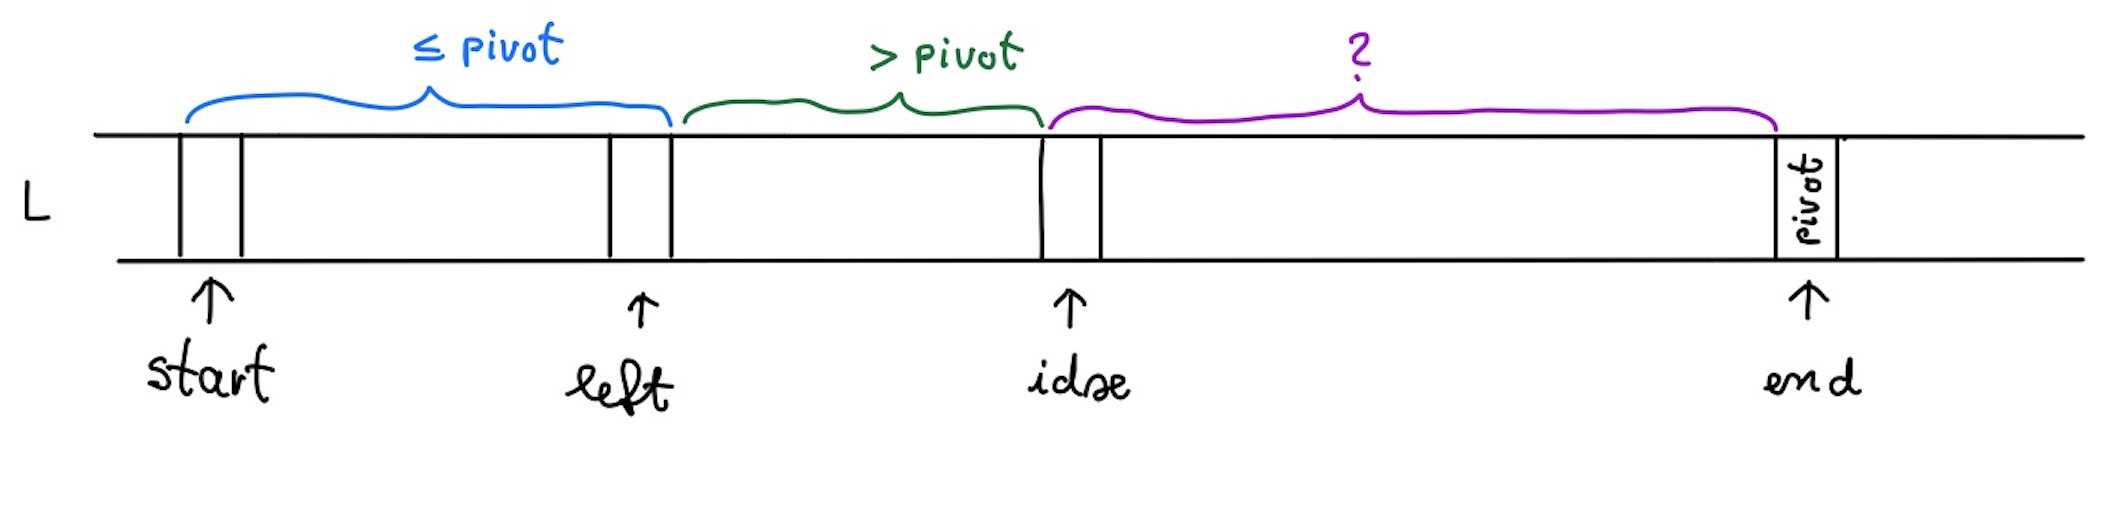
\epsfig{file=Abbildungen/lomuto.png, scale=0.40}} 
  \caption{The invariants of the function \mytt{partition}.}
  \label{fig:lomuto.png}
\end{figure}


      Observe how the invariants (a) and (b) are maintained:
      \begin{enumerate}
      \item Initially, the invariants are true because the corresponding sets are empty.
            At the start of the \mytt{for}-loop we have
            \\[0.2cm]
            \hspace*{1.3cm}
            $\{ \mytt{start}, \cdots, \mytt{left} \} = \{ \mytt{start}, \cdots, \mytt{start} - 1\} = \{\}$
            \\
            and
            \\
            \hspace*{1.3cm}
            $\{ \mytt{left}+1,\cdots,\mytt{idx}-1\} =  \{ \mytt{start},\cdots,\mytt{start}-1\}=\{\}$.
      \item If the element $\mytt{L[idx]}$ is less than the
            pivot element, it need to become part of the subarray $\mytt{L}[\mytt{start}:\mytt{left}+1]$.  In order to
            achieve this, it is placed at the position $\mytt{L}[\mytt{left}+1]$.  The element that has been at
            that position is part of the subarray $\mytt{L}[\mytt{left}+1:\mytt{idx}]$ and therefore,
            most of the times,\footnote{
              It is not always greater than the pivot element
              because the subarray $\mytt{L}[\mytt{left}+1:\mytt{idx}]$ might well be empty.}
            it is greater than the pivot element.  
            Hence we append this element to the end of the subarray
            $\mytt{L}[\mytt{left}+1:\mytt{idx}]$.  After incrementing the index $\mytt{left}$,
            both the placing of the element $\mytt{L[idx]}$ at position $\mytt{left}+1$ and the appending
            of the element $\mytt{L}[\mytt{left}+1]$ to the end of the subarray
            $\mytt{L}[\mytt{left}+1:\mytt{idx}+1]$ is achieved by the statement
            \\[0.2cm]
            \hspace*{1.3cm}
            \mytt{swap(left, idx, L)}.            
      \end{enumerate}
      Once the \mytt{for} loop in line 14 terminates, the call to $\mytt{swap}$ in line 18 moves
      the pivot element into its correct position and returns the index where the pivot element has been
      placed. 
\end{enumerate}


\subsection{Improvements for Quicksort}
There are a number of tricks that can be used to increase the efficiency of \blue{quicksort}.
\begin{enumerate}
\item Instead of taking the first element as the pivot element, use three elements from the list
      $\mytt{L}$ that is to be sorted.  For example, take the first element, the last element, and an
      element from the middle of the list.  Now compare these three elements and take that element as
      a pivot that is the \blue{median} of these elements,  where the \blue{median} \index{median} of three
      elements is defined as the element that lies between the minimum and the maximum of these elements.
      In general, the \blue{median} of a list $L$ of length $2 \cdot n +1$ is defined as the element $x$ such that at
      least $n$ elements of $L$ are less or equal to $x$ and at least $n$ elements are bigger or equal than $x$.
      
      The advantage of this strategy is that the worst case performance is much less likely to occur.  In
      particular,  using this strategy the worst case won't occur for a list that is already
      sorted.
\item If a sublist contains fewer than 10 elements, use \blue{insertion sort} to sort this sublist.

      The paper ``\blue{Engineering a Sort Function}'' by Jon L.~Bentley and M.~Douglas McIlroy
      \cite{bentley:93} describes the previous two improvements.
\item In order to be sure that the average case analysis of \blue{quicksort} holds we can randomly
      \blue{shuffle} the list $L$ that is to be sorted.  This approach is advocated by Sedgewick
      \cite{sedgewick:2011}.  In \textsl{Python} this is quite easy as
      the module \mytt{random} provides a predefined function \mytt{shuffle} that takes a list and shuffles
      it randomly in place.  For example, the code
      \\[0.2cm]
      \hspace*{1.3cm}
      \mytt{L = list(range(10)); random.shuffle(L); print(L)}
      \\[0.2cm]
      might print the result
      \\[0.2cm]
      \hspace*{1.3cm}
      \mytt{[1, 9, 8, 5, 2, 0, 6, 3, 4, 7]}.
\item In 2009, Vladimir Yaroslavskiy introduced \blue{dual pivot quicksort}
      \cite{yaroslavskiy:2009}.\index{dual pivot quicksort}
      His paper can be
      downloaded at the following address:
      \\[0.2cm]
      \hspace*{1.3cm}
      \href{http://codeblab.com/wp-content/uploads/2009/09/DualPivotQuicksort.pdf}{\mytt{http://codeblab.com/wp-content/uploads/2009/09/DualPivotQuicksort.pdf}}
      \\[0.2cm]
      The main idea of Yaroslavskiy is to use two pivot elements $p_1$ and $p_2$.  For example, we can
      define
      \\[0.2cm]
      \hspace*{1.3cm}
      $x := \mytt{L}[0]$, $y := \mytt{L}[-1]$, \quad and then define \quad $p_1 :=\min(x, y)$, $p_2 := \max(x, y)$.
      \\[0.2cm]
      Next, the list $\mytt{L}$ is split into three parts:
      \begin{enumerate}
      \item The first part contains those elements that are less than $p_1$.
      \item The second part contains those elements that are bigger or equal than $p_1$ but less or
            equal than $p_2$.
      \item The third part contains those elements that are bigger than $p_2$.
      \end{enumerate}
      Figure \ref{fig:dual-pivot-quick-sort.stlx} on page \pageref{fig:dual-pivot-quick-sort.stlx}
      shows a simple list-based implementation of \blue{dual pivot quicksort}.

      Various studies have shown that, on average, \blue{dual pivot quicksort} is faster than any other sorting
      algorithm.  For this reason, the version 1.7 of \textsl{Java} uses \blue{dual pivot quicksort}:
      \\[0.2cm]
      \hspace*{0.3cm}
      \href{http://www.docjar.com/html/api/java/util/DualPivotQuicksort.java.html}{http://www.docjar.com/html/api/java/util/DualPivotQuicksort.java.html} 
\end{enumerate}

\begin{figure}[!ht]
\centering
\begin{minted}[ frame         = lines, 
                  framesep      = 0.3cm, 
                  firstnumber   = 1,
                  bgcolor = sepia,
                  numbers       = left,
                  numbersep     = -0.3cm,
                  xleftmargin   = 0.0cm,
                  xrightmargin  = 0.0cm,
                ]{python3}
    def sort(L):
        if len(L) <= 1:
            return L
        x, y, *R   = L
        p1, p2     = min(x, y), max(x,y)
        L1, L2, L3 = partition(p1, p2, R)
        return sort(L1) + [p1] + sort(L2) + [p2] + sort(L3)
    
    def partition(p1, p2, L):
        if L == []:
            return [], [], []
        x, *R      = L
        R1, R2, R3 = partition(p1, p2, R)
        if x < p1:
            return [x] + R1, R2, R3
        if x <= p2:
            return R1, [x] + R2, R3
        else:
            return R1, R2, [x] + R3
\end{minted}
\vspace*{-0.3cm}
\caption{A list based implementation of \blue{dual pivot quicksort}.}
\label{fig:dual-pivot-quick-sort.stlx}
\end{figure}

\exercise
Implement a version of \blue{dual pivot quicksort} that is array-based instead of list-based.
\eoxs


\section{A Lower Bound for the Sorting Problem}
In this section we will show that any sorting algorithm that sorts elements by comparing them must
use at least 
\\[0.2cm]
\hspace*{1.3cm}
 $\Omega\bigl(n \cdot \log_2(n)\bigr)$ 
\\[0.2cm]
comparisons.  The important caveat here is that the sorting algorithm is not permitted to make any assumptions
on the elements of the list $L$ that is to be sorted.  The only operation that is allowed on these
elements is the use of the comparison operator ``\mytt{<}''.  Furthermore, to simplify matters let
us assume that all elements of the list $L$ are distinct.

Let us consider lists of two elements first, i.e.~assume we have
\\[0.2cm]
\hspace*{1.3cm}
$L = [a_1, a_2]$.  
\\[0.2cm]
In order to sort this list, one comparison is sufficient:
\begin{enumerate}
 \item If $a_1 < a_2$, then the list $[a_1, a_2]$ is sorted ascendingly.
 \item If $a_2 < a_1$, then the list $[a_2, a_1]$ is sorted ascendingly.
\end{enumerate}
If the list $L$ that is to be sorted has the form
\\[0.2cm]
\hspace*{1.3cm}
$L = [a_1,a_2,a_3]$,
\\[0.2cm]
then there are 6 possibilities to arrange these elements:
\\[0.2cm]
\hspace*{0.3cm}
$[a_1,a_2,a_3]$, \quad
$[a_1,a_3,a_2]$, \quad
$[a_2,a_1,a_3]$, \quad
$[a_2,a_3,a_1]$, \quad
$[a_3,a_1,a_2]$, \quad
$[a_3,a_2,a_1]$. 
\\[0.2cm]
Therefore, we need at least three comparisons, since with two comparisons we could choose between at most 
four different possibilities.  Next, we generalize this observation.

\begin{Theorem}
Given a list $L$ of $n$ different elements, there are 
\\[0.2cm]
\hspace*{1.3cm}
$\ds n! = 1 \cdot 2 \cdot 3 \cdot {\dots} \cdot (n-1) \cdot n = \prod\limits_{i=1}^n i$ 
\\[0.2cm]
different permutations of $L$. 
\end{Theorem}
\proof The claim is proven by induction on $n$. 
\begin{enumerate}
\item[B.C.:] $n=1$:  

      There is only $1$ way to arrange one element in a list.  As $1! = 1$ the claim is true in this case.
\item[I.S.:] $n \mapsto n+1$:
  
      If we have $n+1$ different elements and want to arrange these elements in a list, then there
      are $n+1$ possibilities for the first element.  In each of these cases the induction
      hypothesis tells us that there are $n!$ ways to arrange the remaining $n$ elements in a list.
      Therefore, all in all there are $(n+1) \cdot n! = (n+1)!$ different arrangements of $n+1$
      elements in a list. \qed
\end{enumerate}
Next, we consider how many different cases can be distinguished if we have $k$ different tests
that only give $\mytt{True}$ or $\mytt{False}$ answers.  Tests of this kind are called \blue{binary tests}.
\begin{enumerate}
\item If we restrict ourselves to binary tests, then one test can only distinguish between two cases.
\item If we have $2$ tests, then we can distinguish between  $2 \cdot 2 = 2^2$ different cases.
\item In general, an easy induction shows that $k$ tests can choose from at most $2^k$ different cases.
\end{enumerate}
The last claim can also be argued as follows:  If the results of the tests are represented as
$0$ and $1$, then $k$ binary tests correspond to a binary string of length
$k$.  However, binary strings of length $k$ can be used to code the numbers from $0$ up to
$2^{k}-1$.  We have
\\[0.2cm]
\hspace*{1.3cm}
$\textsl{card}\bigl(\{0,1,2,\cdots, 2^k-1\}\bigr) = 2^k$.
\\[0.2cm]
Hence there are $2^k$ binary strings of length $k$.  

If we have a list of $n$ different elements, then there are $n!$ different permutations of these
elements.  In order to figure out which of these $n!$ different permutations is given we have to
perform $k$ comparisons, where we must have
\\[0.2cm]
\hspace*{1.3cm}
$2^k \geq n!$.
\\[0.2cm]
This immediately implies
\\[0.2cm]
\hspace*{1.3cm}
$k \geq \log_2(n!)$.
\\[0.2cm]
In order to proceed, we need a lower bound for the expression $\log_2(n!)$.
First, we have
\\[0.2cm]
\hspace*{1.3cm}
$\ds \log_2(n!) = \log_2\left(\prod\limits_{i=1}^n i\right) = \sum\limits_{i=1}^n \log_2(i)$
\\[0.2cm]
The crucial idea is to interpret this sum as an upper \href{https://en.wikipedia.org/wiki/Riemann_sum}{Riemann sum}
of the integral
\\[0.2cm]
\hspace*{1.3cm}
$\ds\int_1^n\log_2(x)\, \mathrm{d}x$
\\[0.2cm]
as is shown in Figure \ref{fig:riemann-sum.pdf}\footnote{
  I have created this figure using the highly recommended tool \href{https://www.geogebra.org/m/h4P4cjsT}{geogebra}.
}.

\begin{figure}[!ht]
  \centering
  \framebox{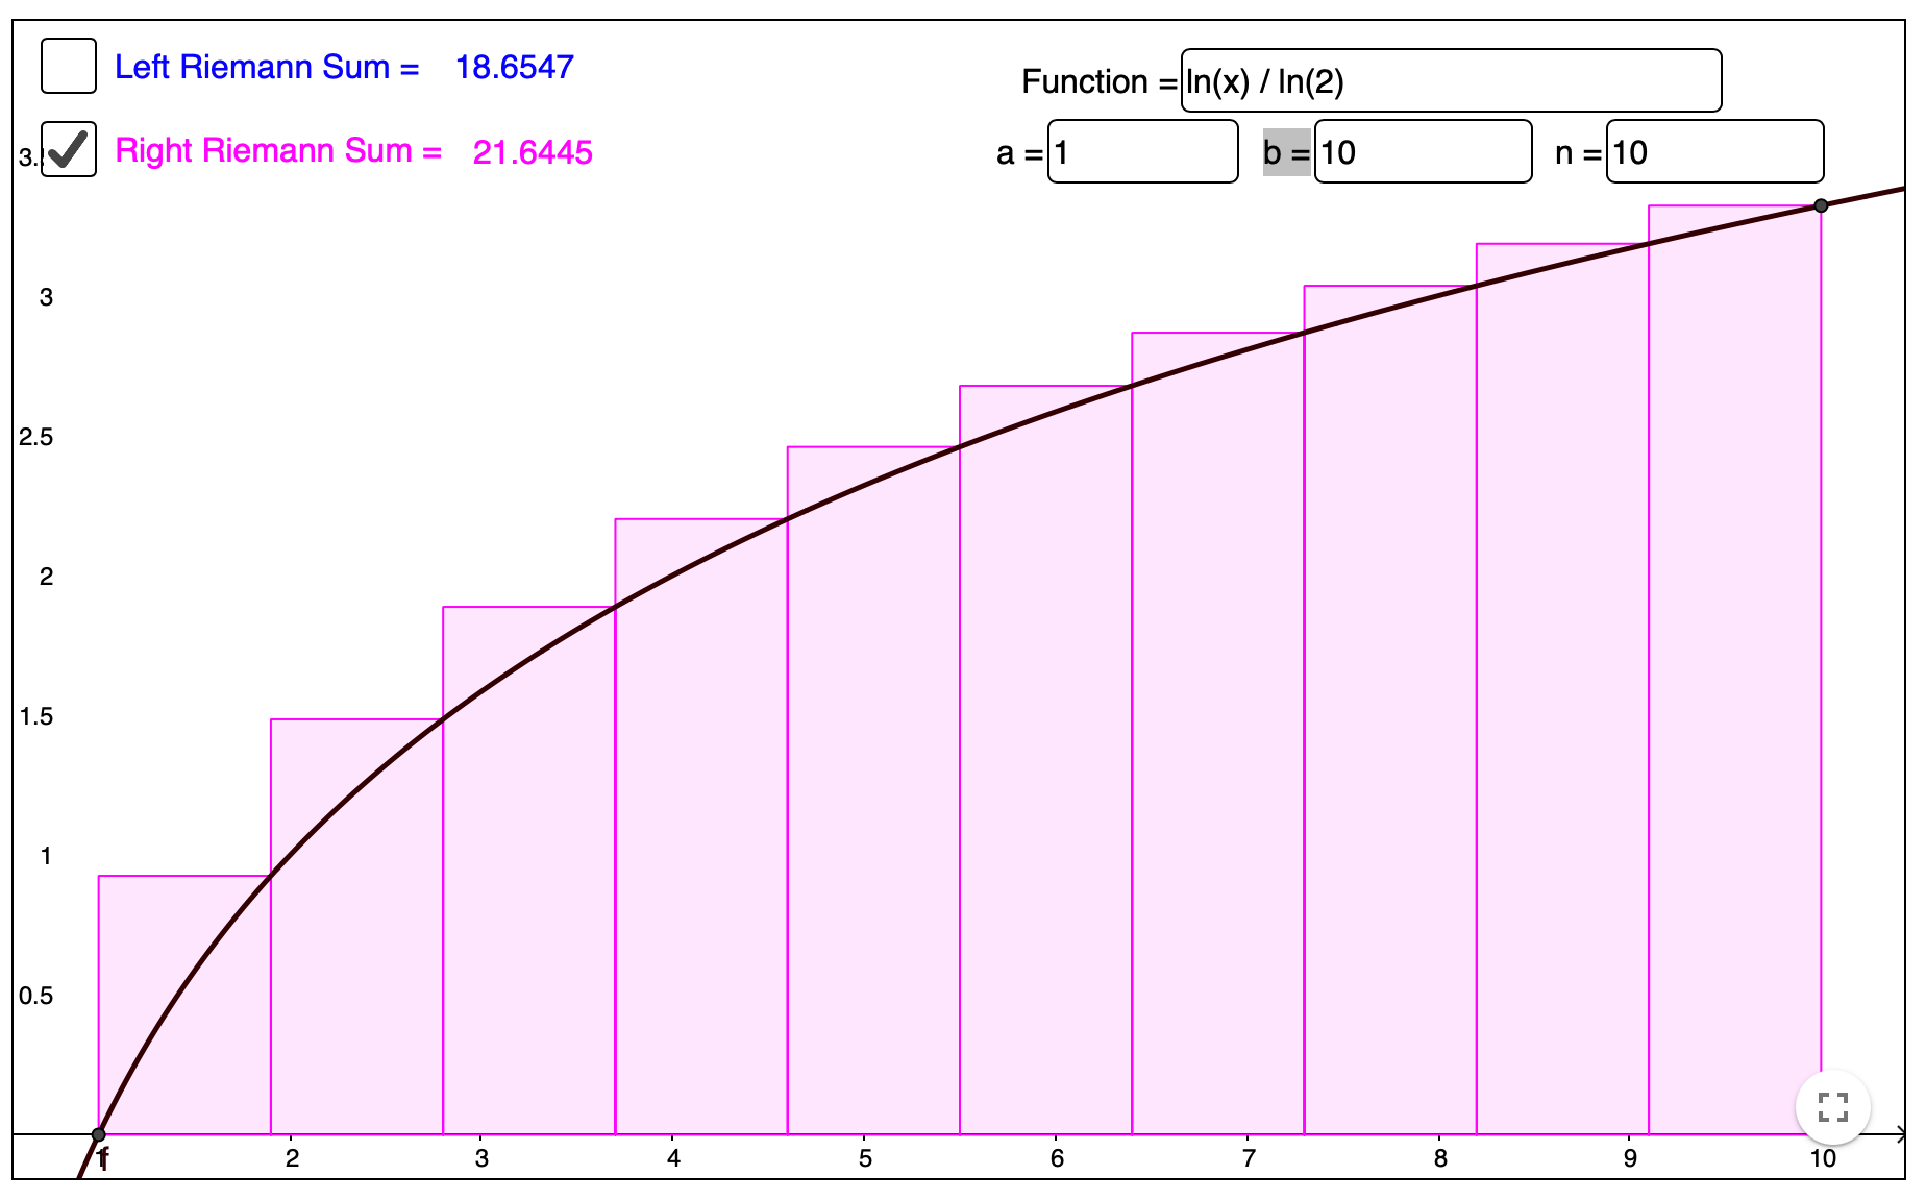
\epsfig{file=Abbildungen/riemann-sum.pdf, scale=0.45}} 
  \caption{The upper sum for the integral $\ds\int\limits_{1}^{10}\log_2(x) \,\mathrm{d}x$.}
  \label{fig:riemann-sum.pdf}
\end{figure}

Therefore we have the following chain of inequations:
\\[0.2cm]
\hspace*{1.3cm}
$
\begin{array}[t]{lcl}
  k & \geq & \ds\log_2(n!) \\[0.2cm]
    & =    & \ds\sum\limits_{i=1}^n \log_2(i) \\[0.5cm]
    & \geq & \ds\int\limits_{1}^n \log_2(x)\, \mathrm{d}x \\[0.2cm]
    & =    & \ds\frac{1}{\,\ln(2)\,} \cdot \int\limits_{1}^n \ln(x)\, \mathrm{d}x  \\[0.2cm]
    & =    & \ds\frac{1}{\,\ln(2)\,} \cdot \bigl[x \cdot \ln(x) - x \bigr]_{1}^n   \\[0.4cm]
    & =    & \ds\frac{1}{\,\ln(2)\,} \cdot \bigl(n \cdot \ln(n) - n + 1\bigr)     \\[0.2cm]
    & =    & \ds n \cdot \log_2(n) - \frac{\,n-1\,}{\,\ln(2)\,}                       
\end{array}
$ 
\\[0.2cm]
This show that
\\[0.2cm]
\hspace*{1.3cm}
$k \geq n \cdot \ds\log_2(n) - \frac{\,n-1\,}{\,\ln(2)\,}$.
\\[0.2cm]
As \blue{merge sort} is able to sort a list of length $n$ using only $n \cdot \log_2(n)$ comparisons
we have shown that this algorithm is optimal with respect to the number of comparisons within a linear bound of
size $(n-1)/\ln(2)$.




\section{Counting Sort}
\index{counting sort}
In the last section of this chapter we introduce a sorting algorithm that has only a \blue{linear} complexity.
According to the result of the previous section this algorithm can not work by comparing the elements of the
list that is to be sorted.  This algorithm only works if the elements of the list that is to be sorted are
natural numbers of a fixed size.  The algorithm is called
\href{https://en.wikipedia.org/wiki/Counting_sort}{counting sort}. We 
explain this algorithm via an example.  Table \ref{tab:marks} on page \pageref{tab:marks} shows a table showing
students and their grades.  As it stands, the names of the students are ordered alphabetically.  However, the
teacher would like to sort the list of students according to their grades.  Within a group of students that
have achieved the same grade, the students should still be ordered alphabetically.  Table
\ref{tab:marks-sorted} on page \pageref{tab:marks-sorted} shows the table that has been sorted accordingly.

\begin{table}[!ht]
  \centering
  \begin{tabular}{|l|c|}
    \hline
    Student   & Grade \\
    \hline
    \hline
    Alexander & 4 \\
    \hline
    Benjamin  & 2 \\
    \hline
    Daniel    & 3 \\
    \hline
    David     & 3 \\
    \hline
    Elijah    & 2 \\
    \hline
    Gabriel   & 1 \\
    \hline
    Henry     & 2 \\
    \hline
    Jacob     & 5 \\
    \hline
    James     & 3 \\
    \hline
    Joseph    & 2 \\
    \hline
    Liam      & 2 \\
    \hline
    Logan     & 3 \\
    \hline
    Lucas     & 1 \\
    \hline
    Mason     & 2 \\
    \hline
    Matthew   & 5 \\
    \hline
    Michael   & 3 \\
    \hline
    Noah      & 4 \\
    \hline
    Oliver    & 2 \\
    \hline
    Owen      & 4 \\
    \hline
    Samuel    & 3 \\
    \hline
    Sebastian & 2 \\
    \hline
    William   & 1 \\
    \hline
  \end{tabular}
  \caption{Students and their grades, sorted alphabetically.}
  \label{tab:marks}
\end{table}

\begin{table}[!ht]
  \centering
  \begin{tabular}{|l|c|}
    \hline
    Student   & Grade \\
    \hline
    \hline
    Gabriel   & 1 \\
    \hline
    Lucas     & 1 \\
    \hline
    William   & 1 \\
    \hline
    Benjamin  & 2 \\
    \hline
    Elijah    & 2 \\
    \hline
    Henry     & 2 \\
    \hline
    Joseph    & 2 \\
    \hline
    Liam      & 2 \\
    \hline
    Mason     & 2 \\
    \hline
    Oliver    & 2 \\
    \hline
    Sebastian & 2 \\
    \hline
    Daniel    & 3 \\
    \hline
    David     & 3 \\
    \hline
    James     & 3 \\
    \hline
    Logan     & 3 \\
    \hline
    Michael   & 3 \\
    \hline
    Samuel    & 3 \\
    \hline
    Alexander & 4 \\
    \hline
    Noah      & 4 \\
    \hline
    Owen      & 4 \\
    \hline
    Jacob     & 5 \\
    \hline
    Matthew   & 5 \\
    \hline
  \end{tabular}
  \caption{Students and their grades, sorted with respect to the grade.}
  \label{tab:marks-sorted}
\end{table}
We proceed to describe an algorithm that is capable of transforming Table \ref{tab:marks} into Table
\ref{tab:marks-sorted}.  This algorithm works in three stages.
\begin{enumerate}
\item The first stage is the \blue{counting stage}.  In this stage we count the number of students
      that have a specific grades.  In the example from Table \ref{tab:marks} we find the following:
      \begin{enumerate}[(a)]
      \item 3 students have grade 1.
      \item 8 students have grade 2.
      \item 6 students have grade 3.
      \item 3 students have grade 4.
      \item 2 students have grade 5.
      \end{enumerate}
\item The second stage is the \blue{indexing stage}.  In this stage our goal is compute the indices of the
      sublists containing the different grades.  For example, since there are 3 students with a grade of $1$
      and $1$ is the smallest grade, we know that the students with grade $1$ will be found in the sublist
      $\mytt{L[0:3]}$.  Similarly, as there are $8$ students that have a grade of $2$ and $3 + 8 = 11$,
      the sublist $\mytt{L[3:11]}$ will contain the students with grade $2$.
      All in all, we have the following:
      \begin{enumerate}[(a)]
      \item The sublist $\mytt{L[0:3]}$ contains the students with grade 1.
      \item The sublist $\mytt{L[3:11]}$ contains the students with grade 2.
      \item The sublist $\mytt{L[11:17]}$ contains the students with grade 3.
      \item The sublist $\mytt{L[17:20]}$ contains the students with grade 4.
      \item The sublist $\mytt{L[20:22]}$ contains the losers.
      \end{enumerate}
      The indexing stage computes the \blue{starting indices} of these sublists.
      Of course,  the first sublist has to start at the index $0$.  Since there are 3 students with a grade of 1,
      the second sublist starts at the index $0 + 3 = 3$.  Since there are 8 students with a grade of 2, the third
      sublist starts at the index $0 + 3 + 8 = 11$.  In general, if the sublist for the students with grade $g$
      starts at index $i_g$ and there are $n_g$ students that have achieved the grade $g$, then the sublist for the
      students with grade $g+1$ starts at index $i_{g+1}$ where
      \\[0.2cm]
      \hspace*{1.3cm}
      $\ds i_{g+1} = i_g + n_g$.
\item The \blue{distribution stage} iterates over the list of students and inserts them into the sublists
      corresponding to the grades of the students.
\end{enumerate}
Figure \ref{fig:counting-sort.stlx} on page \pageref{fig:counting-sort.stlx} shows an implementation of
counting sort.  We proceed to discuss this algorithm line by line.

\begin{figure}[!ht]
\centering
\begin{minted}[ frame         = lines, 
                  framesep      = 0.3cm, 
                  firstnumber   = 1,
                  bgcolor = sepia,
                  numbers       = left,
                  numbersep     = -0.2cm,
                  xleftmargin   = 0.8cm,
                  xrightmargin  = 0.8cm,
                ]{python3}
    def countingSort(Students):
        maxGrade =    255
        Counts   =    [0] * (maxGrade+1)
        Index    = [None] * (maxGrade+1)
        Sorted   = [None] * len(Students)
        # Phase 1: Counting
        for _name, grade in Students:
            Counts[grade] += 1
        # Phase 2: Indexing
        Index[0] = 0
        for grade in range(maxGrade):
            Index[grade+1] = Index[grade] + Counts[grade]
        # Phase 3: Distribution
        for name, grade in Students:
            idx           = Index[grade]
            Sorted[idx]   = (name, grade)
            Index[grade] += 1
        return Sorted
\end{minted}
\vspace*{-0.3cm}
\caption{An implementation of \blue{counting sort}.}
\label{fig:counting-sort.stlx}
\end{figure}

\begin{enumerate}
\item The procedure \mytt{countingSort} receives one argument.  The list $\mytt{Students}$
      is a list of pairs of the form $\mytt{(name, grade)}$ where
      \begin{enumerate}
      \item \mytt{name}  is the name of a student, while
      \item \mytt{grade} is the grade that this student has achieved.
      \end{enumerate}
      The list $\mytt{Students}$ is sorted alphabetically w.r.t.~the names of the students.
      The purpose of the function \mytt{countingSort} is to sort this list according to their grades.
      Sublists of students with the same grade should still be sorted alphabetically.
\item In order for our function to generalize to arbitrary numbers we will assume that all grades are elements
      of the set $\{0,\cdots,255\}$.  Therefore we define $\mytt{maxGrade}$ as $255$.
      Of course, in the example discussed so far we know that the largest
      grade is $5$.  However, we will use the function $\mytt{countingSort}$ later as an auxiliary function
      when implementing \blue{radix sort}.  Then the grades will be bytes and hence be natural numbers less
      or equal than $255$.
\item Next, we initialize the auxiliary array \mytt{Count} to be an array of length $\mytt{maxGrade}+1$.
      Later, for a grade $g$ the number $\mytt{Counts}[g]$ will contain the number of students that have
      attained the grade $g$.  Initially, all entries of the array \mytt{Count} are set to $0$.
\item After the indexing stage, the array \mytt{Index} will contain the start indices of the different sublists.
      For a grade $g$, $\mytt{Index}[g]$ is the first index of the sublist containing those students that
      have achieved the grade $g$.
\item The list \mytt{Sorted} is the list that will be returned as the result.
      This list will contain pairs of the form \mytt{(name, grade)} where \mytt{name} is the name of a student
      and \mytt{grade} is her grade.
\item The \mytt{for}-loop in line 7-8 performs the \blue{counting stage}.  We iterate over all grades
      in the list \mytt{Students} and increment the counter $\mytt{Counts}[\mytt{grade}]$ that is associated with the given grade.
\item Next, the index for the start of the sublist containing those students that have achieved the grade $0$
      is initialized as $0$ in line 10. 
\item Then, the \mytt{for}-loop in line 11-12 performs the \blue{indexing stage}. As the number
      $\mytt{Index}[\mytt{grade}]$ is the index of the start of the sublist for those students that have
      achieved the grade  $\mytt{grade}$ and the number of these
      students is $\mytt{Counts}[\mytt{grade}]$, the sublist of the students with grade $\mytt{grade}+1$
      has to start at index 
      \\[0.2cm]
      \hspace*{1.3cm}
      $\mytt{Index}[\mytt{grade}] + \mytt{Counts}[\mytt{grade}]$.
\item Finally, the \mytt{for}-loop in line 14-17 performs the \blue{distribution stage}.
      \begin{enumerate}
      \item The \mytt{for}-loop iterates over all students. 
      \item We need to find where to put a student with grade \mytt{grade}.
            $\mytt{Index}[\mytt{grade}]$ gives us the \mytt{index} of the next free entry in the
            result list \mytt{Sorted} corresponding for this grade.
      \item In line 16 the students name and her grade are stored in the result lists \mytt{Sorted}
            at the index $\mytt{idx}$.
      \item Finally, we need to increment the index stored at $\mytt{Index}[\mytt{grade}]$ since we have
            just used this index and therefore the next student with the same grade needs to be
            stored at the subsequent location.  This is done in line 17.
      \end{enumerate}
\end{enumerate}
If the list \mytt{Students} has a length of $n$, then it is easy to
see that counting sort has the complexity $\Oh(n)$.  The first \mytt{for}-loop iterates over the list \mytt{Students} so
its body is executed $n$ times.  The second for loop iterates 255 times and the last \mytt{for}-loop again
iterates $n$ times.  Hence, counting sort is a \blue{linear sorting algorithm}.  Note that we do not compare grades in
order to sort them.

Another important fact is that counting sort is \blue{stable}\index{stable}: In the resulting list, the sublists
corresponding to the different grades are still sorted alphabetically.  This is so because these sublists are
filled by iterating over the original list that is sorted alphabetically.  If two students $x$ and $y$ have the
same grade $g$ but the name of $x$ is alphabetically before the name of $y$, then $x$ will be inserted into the
sublist corresponding to grade $g$ before $y$ and hence these sublists are still ordered alphabetically.  This property
is crucial for the development of our next sorting algorithm \blue{radix sort}.

\section{Radix Sort}
\index{radix sort}
The importance of the previous sorting algorithm, \blue{counting sort}, stems from the fact that it is part of the
implementation of \href{https://en.wikipedia.org/wiki/Radix_sort}{radix sort}. \index{radix sort}
\blue{Radix sort} was used as early as 1887 in 
\href{https://en.wikipedia.org/wiki/Tabulating_machine}{tabulating machines} constructed by
\href{https://en.wikipedia.org/wiki/Herman_Hollerith}{Hermann Hollerith}.  \index{Hollerith, Herman} He was the founder of
the \blue{Tabulating Machine Company} that later became \href{https://en.wikipedia.org/wiki/IBM}{\textsc{Ibm}}.
To understand radix sort, suppose we want to implement an algorithm that sorts a large number of 32 bit
unsigned integers.  The easiest way to do this would be to use counting sort:
The main idea of radix sort is to split the
32 bit numbers into four chunks of 8 bits each and to use each of these four chunks as a grade.  To formulate this
mathematically, a 32 bit unsigned integer $x$ is defined via its four bytes $b_1$, $\cdots$, $b_4$ as follows:
\\[0.2cm]
\hspace*{1.3cm}
$\ds x = b_4 \cdot 256^{3} + b_3 \cdot 256^{2} + b_2 \cdot 256^{1} + b_1$.
\\[0.2cm]
Note that we have numbered the bytes starting from the the least significant byte.
Then, radix sort works as follows:
\begin{enumerate}
\item Sort the numbers by interpreting the byte $b_1$ as a grade.
\item Take the numbers that have been sorted by the byte $b_1$ and sort them according to the byte $b_2$ next.
      Since counting sort is \blue{stable}, numbers which happen to have the same byte $b_2$ will still be
      sorted with respect to the byte $b_1$.  Hence, after the sorting with respect to the byte $b_2$ is
      complete, in effect the numbers will then be sorted according to both $b_2$ and $b_1$.
\item Next, use counting sort to sort the numbers with respect to the byte $b_3$.
\item Finally, use counting sort to sort the numbers with respect to the byte $b_4$.  By the stability of
      counting sort, the numbers are now sorted with respect to all of their byte, where $b_4$ is the most
      significant byte and $b_1$ is the least significant byte. Hence, the numbers are sorted. 
\end{enumerate}


\begin{figure}[!ht]
\centering
\begin{minted}[ frame         = lines, 
                  framesep      = 0.3cm, 
                  firstnumber   = 1,
                  bgcolor = sepia,
                  numbers       = left,
                  numbersep     = -0.2cm,
                  xleftmargin   = 0.8cm,
                  xrightmargin  = 0.8cm,
                  ]{python3}
    def extractByte(n, k):
        return n >> (8 * (k-1)) & 0b11111111
    
    def radixSort(L):
        L = [(n, 0) for n in L]
        for k in range(1, 4+1):
            L = [(n, extractByte(n, k)) for (n, _) in L]
            L = countingSort(L)
        return [n for (n, _) in L]    
\end{minted}
\vspace*{-0.3cm}
\caption{An implementation of \blue{radix sort} for sorting unsigned 32 integers.}
\label{fig:radix-sort.stlx}
\end{figure}
Figure \ref{fig:radix-sort.stlx} on page \pageref{fig:radix-sort.stlx} shows an implementation of radix
sort that implements this idea.
\begin{enumerate}
\item The function \mytt{extractByte} is called with two arguments:
      \begin{enumerate}[(a)]
      \item $n$ is supposed to be an unsigned 32 bit number.  Hence $n$ is a integer satisfying $0 \leq n < 2^{32}$.
      \item $k$ is the index of the byte that is to be extracted.  It is supposed that the least significant
            byte has the index $1$.
      \end{enumerate}
      Hence, $\mytt{extractByte}(n, k)$ extracts the $k$-th byte of the number $n$.

      \mytt{extractByte} works by shifting the number $x$ by $(k-1) \cdot 8$ bits to the right using the shift
      operator ``\mytt{>>}''.  This shift removes all bytes with index less than $k$. Then, the least significant
      byte of the remaining number is extracted using the  \blue{bitwise and operator} ``\mytt{\&}'' with the
      mask $255$.  Note that $255$ is written as $11111111_2$ in binary and hence can be used to extract the
      eight least significant bits of a number. 
\item \mytt{radixSort} takes a list of unsigned 32 bit integers $L$ as its arguments.
\item This list is extended to a list of pairs where the first component of each pair is the number.      
\item Then \mytt{radixSort} iterates over the four bytes of the numbers of the list $L$ starting with the
      least significant byte.
\item In line 7 the $k^\mathrm{th}$ byte of the numbers of $L$ is written into the second component
      of the pairs stored in the list.      
\item With respect to \mytt{countingSort},  the elements of the list given to \mytt{countingSort} as its
      first argument are 
      arbitrary objects.  Therefore, it does not matter whether the first argument to the function
      \mytt{countingSort} is a list of strings interpreted as student names or a list of numbers.
      Therefore in line 8 this list
      is sorted with respect to the $k^\mathrm{th}$ byte. 
\item When $L$ is returned, this list is sorted with respect to all of the four bytes making up its numbers and
      hence, it is sorted.
\end{enumerate}

\section{Application: Handwritten Digit Recognition}
\index{digit recognition}
In the last section of this chapter we discuss an application of sorting:
\blue{recognizing handwritten digits}.\index{handwritten digit recognition}
We will use a \blue{training set} of $50,000$ handwritten digits. Figure \ref{fig:digits.pdf} shows the first 24
images of these handwritten digits.  These images are given as grey scale images of $28 \times 28$ pixels.
Each pixel $p$ is a floating point number satisfying $0 \leq p \leq 1$. If $p = 1.0$, the pixel is completely
black, while $p = 0.0$ if the pixel is white.  Furthermore, for each of these images we also have been given a
\blue{label} $d \in \{0,1,2,\cdots,9\}$, which specifies the digit that is represented in the image.  Besides the training set 
there is also a \blue{test set} of $10,000$ of handwritten images.  Our task is to \blue{classify} the images
of this test set as digits, i.e.~for each image of the test set we want to recognize the digit that is depicted.


\begin{figure}[!ht]
  \centering
  \framebox{\epsfig{file=Abbildungen/digits.pdf, scale=0.60}} 
  \caption{The first 24 digits of our dataset.}
  \label{fig:digits.pdf}
\end{figure}

\subsection{The $k$-Nearest Neighbour Algorithm}
We will use the \href{https://en.wikipedia.org/wiki/K-nearest_neighbors_algorithm}{$k$-nearest neighbours algorithm} 
\index{$k$-nearest neighbours algorithm}
to solve this task.  Given an image $x$ that is to be classified as a digit, we look at those images in the
training set that are somehow \blue{close} to $x$.  If these images are all labelled with the same digit $d$,
we conclude that $x$ shows the digit $d$.  In order to implement this algorithm, we have to specify what it
means for an image $\mathbf{x}$ to be close to another image $\mathbf{y}$.  As the images have a size of $28 \times 28 = 784$
pixels, they can be viewed as $784$-dimensional vectors.  We can compute the \blue{Euclidean distance}
$d(\mathbf{x}, \mathbf{y})$ between $\mathbf{x}$ and $\mathbf{y}$ using the formula
\\[0.2cm]
\hspace*{1.3cm}
$\ds d(\mathbf{x}, \mathbf{y}) := \sqrt{\sum\limits_{i=1}^n (x_i - y_i)^2\;}$.
\\[0.2cm]
This formula is a generalization of the distance between two points $(x_1, x_2)$ and $(y_1, y_2)$ in the the
plane $\mathbb{R}^2$, which, according to the \href{https://en.wikipedia.org/wiki/Pythagorean_theorem}{Pythagorean theorem}, is given as 
\\[0.2cm]
\hspace*{1.3cm}
$\sqrt{(x_1 - y_1)^2 + (x_2 - y_2)^2\;}$.
\\[0.2cm]
Given an image $\mathbf{y}$ that needs to be classified and a training set of $n$ labelled images, the $k$-nearest
neighbours algorithm works as follows: 
\begin{enumerate}[(a)]
\item For every image $\mathbf{x}$ in the training set compute the Euclidean distance $d(\mathbf{x},
  \mathbf{y})$ between $\mathbf{x}$ and $\mathbf{y}$.
\item \blue{Sort} the images in the training set according to their distance to $\mathbf{y}$.
\item Pick those $k$ images that have the smallest distances to $\mathbf{y}$.
      These $k$ images are called the \blue{$k$ nearest neighbours}.
\item Among the $k$ nearest neighbours, pick the label that occurs most frequently.
      
      For example, if $k=7$ and $3$ of the $7$ nearest neighbours are labelled as the digit $3$, while $2$ are
      labelled as the digit $2$ and $2$ are labelled as the digit $1$, then we conclude that the image
      $\mathbf{y}$ shows the digit $3$. 
\end{enumerate}

\begin{figure}[!ht]
\centering
\begin{minted}[ frame         = lines, 
                 framesep      = 0.3cm, 
                 firstnumber   = 1,
                 bgcolor       = sepia,
                 numbers       = left,
                 numbersep     = -0.3cm,
                 xleftmargin   = 0.0cm,
                 xrightmargin  = 0.0cm,
               ]{python3}
    import gzip
    import pickle
    import numpy as np

    def load_data():
        with gzip.open('mnist.pkl.gz', 'rb') as f:
            train, _, test = pickle.load(f, encoding="latin1")
        return (train[0], test[0], train[1], test[1])
        
    X_train, X_test, Y_train, Y_test = load_data()
        
    def distance(x, y):
        return np.sqrt(np.sum((x - y)**2))
    
    def maxCount(L):
        Frequencies         = {}    # number of occurrences 
        most_frequent       = L[0]  # most frequent digit so far
        most_frequent_count = 1     
        for d in L:
            if d in Frequencies:
                Frequencies[d] += 1
            else:
                Frequencies[d]  = 1
            if Frequencies[d] > most_frequent_count:
                most_frequent       = d
                most_frequent_count = Frequencies[d]
        return most_frequent, most_frequent_count / len(L)
    
    def digit(x, k):
        n          = X_train.shape[0]  # number of all training images
        Distances  = [(distance(X_train[i,:], x), i) for i in range(n)]
        Neighbours = [Y_train[i] for _, i in sorted(Distances)]
        return maxCount(Neighbours[:k])

    digit(X_test[0,:], 13)
\end{minted}
\vspace*{-0.3cm}
\caption{The $k$-nearest neighbours algorithm for digit recognition.}
\label{fig:Digit-Recognition.ipynb}
\end{figure}

\noindent
Figure \ref{fig:Digit-Recognition.ipynb} on page \pageref{fig:Digit-Recognition.ipynb} shows a program that can
be used to recognize a handwritten digit.
\begin{enumerate}
\item The images of the handwritten digits are stored in the file \mytt{mnist.pkl.gz}.  This file is compressed
      using \mytt{gzip} and the images have been \blue{pickled} using the module
      \mytt{pickle}\index{pickle}.  The module
      \mytt{pickle} supports the reading and writing of \textsl{Python} data structures and is therefore
      used to make data \blue{persistent}, i.e.~to store the data structures of a program in a file system.
      The counterpart of the function \mytt{load} is the function \mytt{dump}.

      In order to read the images of the handwritten digits, we therefore have to import the modules
      \mytt{gzip} and \mytt{pickle}.  The module \mytt{numpy} is needed as these images are stored as
      \mytt{numpy} \blue{arrays}.  
\item The function $\mytt{load\_data}()$ returns a tuple of the form
      \\[0.2cm]
      \hspace*{1.3cm}
      $ \ds (\mytt{X\_train}, \mytt{X\_test}, \mytt{Y\_train}, \mytt{Y\_test}) $
      \\[0.2cm]
      where 
      \begin{enumerate}[(a)]
      \item $\mytt{X\_train}$ is a matrix storing the 50,000 training images of handwritten digits.
            For each $i \in \{0,\cdots,49\,999\}$ the row $\mytt{X\_train}[i, :]$ is an array of size $784$ storing a single image.
      \item $\mytt{X\_test}$ is a matrix containing 10,000 images of handwritten digits that we will use to
            test our implementation.
      \item $\mytt{Y\_train}$ is an array of size 50,000. For each $i \in \{0,\cdots,49\,999\}$ the number $\mytt{Y\_train}[i]$
            specifies the digit shown in the $i$th training image.
      \item $\mytt{Y\_test}$ is an array of size 10,000. For each $i \in \{0,\cdots,9\,999\}$ the number $\mytt{Y\_test}[i]$
            specifies the digit shown in the $i^{\mathrm{th}}$ test image.
      \end{enumerate}
      The function \mytt{open} from the module \mytt{gzip} opens the specified file and automatically
      decompresses it.  In the file \mytt{mnist.pkl.gz} the data is stored as a triple of pairs.
      For our purposes, we only need the first and the last component of this triple.  Each of these components
      is a pair of the form $(\textsl{data}, \textsl{label})$, where \textsl{data} is an array of images and
      \textsl{labels} is an array specifying the digits represented in these images.
      The function \mytt{load\_data} extracts the data stored in these pairs.
\item The function $\mytt{distance}(x, y)$ computes the Euclidean distance between the images $x$ and $y$.
      Given a vector $x$, the expression $x \mytt{**} 2$ computes a vector containing the squares of the
      components of $x$.  These squares can then be summed using the \mytt{numpy} function \mytt{sum}.
\item Given a list $L$ of digits, the function $\mytt{maxCounts}(L)$ returns a pair $(d, p)$ where $d$ is the digit that occurs most frequently in $L$
      and $p$ is the fraction of occurrences of $d$ in $L$.  For example, we have
      \\[0.2cm]
      \hspace*{1.3cm}
      $\mytt{maxCounts}([5,2,3,5,2,5,6,5,7,8]) = (5, 0.4)$
      \\[0.2cm]
      because the digit $5$ is the most frequent digit in the list $[5,2,3,5,2,5,6,5,7,8]$ and $40$\%
      of the digits in this list are fives.  In detail, the function \mytt{maxCounts} works as follows:
      \begin{enumerate}[(a)]
      \item \mytt{Frequencies} is a dictionary that specifies how often a digit $d$ occurs in the list $L$.
      \item \mytt{most\_frequent} is the digit that so far is known to be the most frequent digit in $L$.
            Initially, this is assumed to be the first digit.  As we iterate over the list $L$, this variable
            is updated.
      \item \mytt{most\_frequent\_count} is the number of occurrences of the digit \mytt{most\_frequent}.
      \item As we iterate over the digits in $L$ we update their frequencies.  If we encounter a digit that is
            more common than the digit stored in the variable \mytt{most\_frequent} we update this variable
            and the associated value \mytt{most\_frequent\_count}.
      \end{enumerate}
\item Given an image of a digit stored in the vector $\mathbf{x}$ and a number of neighbours $k$, the function
      $\mytt{digit}(\mathbf{x}, k)$ computes those $k$ images in the training set \mytt{X\_train} that are
      \blue{closest} to the image $\mathbf{x}$, where \blue{closeness} of images is defined in terms of the
      \blue{Euclidean distance} of the vectors that store these images.  From these $k$ closest images of the training
      set the function chooses the digit that occurs most frequently.  It returns a pair $(d, p)$ where $d$
      is the digit that is most frequently occurring in the list of $k$ neighbours and $p$ is the percentage
      of images in the $k$ neighbours of $\mathbf{x}$ that show the digit $d$.  The implementation works as follows:
      \begin{enumerate}[(a)]
      \item \mytt{n} is the number of training examples.  In our case, $n = 50,000$.
      \item \mytt{Distances} is a list of pairs of the form $(d, i)$, where $d$ is the distance
            of the $i$-th image in the training set from the given image $x$.
      \item These pairs are \blue{sorted} with respect to their distance and the labels corresponding to the
            images are computed.  Therefore, \mytt{Neighbours} is a list of the labels of all $50,000$
            training images sorted according to their distance to the given image $x$.
      \item Finally, the function \mytt{maxCounts} takes the $k$ closest images and computes the digit that
            is most frequently occurring.
      \end{enumerate}
\item The last line shows how the function \mytt{digit} can be used to classify the first image from the test
      set using the 13 closest neighbours. 
\end{enumerate}
\pagebreak

\exercise
In the program shown in Figure \ref{fig:Digit-Recognition.ipynb} on page \pageref{fig:Digit-Recognition.ipynb}
we have sorted the list \mytt{Distances} in line 32.  The only reason to do this was to be able to find the $k$ smallest
distances in this list.  As $k$ is a small number and the list \mytt{Distances} is rather large, this seems wasteful.
\begin{enumerate}[(a)]
\item Devise an algorithm Quickselect that selects the $k$ smallest elements from a list $L$.

      \hint
      Try to adapt the algorithm Quicksort so that instead of sorting the list it finds the $k$ smallest elements.      
\item Analyse the average complexity of your algorithm.

      \hint
      The recurrence equation resulting from an efficient implementation of Quickselect is quite complicated.
      Instead of solving this recurrence equation it is sufficient if you are able to prove by induction on the
      length $n$ of the list $L$ that your algorithm uses at most $4 \cdot n$ comparisons in order to compute
      the $k$ smallest elements.
      \eox
\end{enumerate}   
\pagebreak

\section{Check Your Understanding}
If you are able to answer the questions below confidently, then you can assume that you have mastered the concepts
introduced in this chapter.
\begin{enumerate}
\item How have we defined the concept of a \blue{linear order}?
\item What type of order do we need if we have to sort a list?
\item Describe the algorithm \blue{insertion sort} on an abstract mathematical level.
\item What is the complexity of \blue{insertion sort}?
\item Is there a case where \blue{insertion sort}  has only a linear complexity?
\item Describe the algorithm \blue{selection sort} on an abstract mathematical level.
\item What is the complexity of \blue{selection sort}?
\item Compare the complexity of \blue{selection sort} with the complexity of \blue{insertion sort}.
\item Describe the algorithm \blue{merge sort} on an abstract mathematical level.
\item Describe an array-based, non-recursive implementation of \blue{merge sort}.
\item Describe the algorithm \blue{quicksort} on an abstract mathematical level.
\item Describe an array-based implementation of \blue{quicksort}.
\item Compare the complexity of \blue{merge sort} with the complexity of \blue{quicksort}.
\item Compare the memory requierements of \blue{merge sort} and \blue{quicksort}.
\item Describe \blue{dual pivot quicksort}.
\item In which case is \blue{dual pivot quicksort} much faster than \blue{quicksort}?
\item How does \blue{counting sort} work?
\item How does \blue{radix sort} work?
\item What is the complexity of \blue{radix sort}?
\item How does the \blue{$k$-nearest neighbours algorithm} work?
\end{enumerate}

%%% Local Variables: 
%%% mode: latex
%%% TeX-master: "algorithms"
%%% End: 

%\include{timsort}  // how sorting is done in practice in python
\chapter{Abstract Data Types}
In the same way as the notion of an \blue{algorithm} abstracts from the details of a concrete
implementation of this algorithm, the notion of an \href{https://en.wikipedia.org/wiki/Abstract_data_type}{abstract data type} abstracts from the implementation
details of concrete data structures.  Therefore, this notion enables us to separate algorithms from the data
structures used in these algorithms.  This chapter is structured as follows:
\begin{enumerate}[(a)]
\item We start with the formal definition of an abstract data types.  
\item As an example of an abstract data types we introduce
      \href{https://en.wikipedia.org/wiki/Stack_(abstract_data_type)}{stacks}. 
\item Then we show how abstract data types are supported in \textsl{Python} via \blue{classes}.  
\item Next, we demonstrate how stacks can be used to evaluate \blue{arithmetic expressions}.  To this end we build an
      \href{https://en.wikipedia.org/wiki/Operator-precedence_parser}{operator precedence parser}. 
\item Finally, we discuss the benefits of abstract data types.
\end{enumerate}
Abstract data types were proposed by 
\href{https://en.wikipedia.org/wiki/Barbara_Liskov}{Barbara Liskov}\footnote{
  Barbara Liskov received the 2008 \href{https://en.wikipedia.org/wiki/Turing_Award}{Turing Award}.
} \index{Liskov, Barbara}
and Stephen Zilles in 1974 \cite{liskov:1974}.  Abstract data type are one of the two main ingredients of
\blue{object oriented programming}.  They were first implemented in the programming language
\href{https://en.wikipedia.org/wiki/CLU_(programming_language)}{\textsc{Clu}}. \index{\textsc{Clu}}
The other ingredient of object oriented programming is \blue{inheritance}.

\section[Formal Definition]{A Formal Definition of Abstract Data Types}
We define an \blue{abstract data type} $\mathcal{D}$ formally as a 5-tupel of the form \index{abstract data type}
\\[0.2cm]
\hspace*{1.3cm}
 $\mathcal{D} = \langle N, P, \textsl{Fs}, \textsl{Ts}, \textsl{Ax} \rangle$,
\\[0.2cm] 
where the meaning of the components is as follows:
\begin{enumerate}
\item $N$ is a string.  This string is the \blue{name} of the abstract data type. 
\item $P$ is the set of \blue{type parameters}.   Here, a type parameter is just a string.
      This string is interpreted as a type variable.  The idea is that we can later substitute 
      a data type for this string. \index{type parameter}
\item $\textsl{Fs}$ is the set of \blue{function symbols}.  These function symbols denote the 
      operations that are supported by this abstract data type. The function symbols itself are strings.
\item $\textsl{Ts}$ is a set of \blue{type specifications}.  For every function symbol
      $f \in \textsl{Fs}$
      the set $\textsl{Ts}$ contains a \blue{type specification}\index{type specification} of the form 
      \\[0.2cm]
      \hspace*{1.3cm} 
      $f: T_1 \times \cdots \times T_n \rightarrow S$. 
      \\[0.2cm]
      Here,  $T_1$, $\cdots$, $T_n$ and $S$ are names of data types.  There are three cases for
      these data types: 
      \begin{enumerate}
      \item We can have predefined data types like, e.g.~``\texttt{int}'' or ``\texttt{str}''.
      \item Furthermore, $T_1$, $\cdots$, $T_n$ and $S$ can be the names of abstract data types.
      \item Finally,  $T_1$, $\cdots$, $T_n$ and $S$ can be type parameters from the set $P$.
      \end{enumerate}
      The type specification $f: T_1 \times \cdots \times T_n \rightarrow S$ expresses the fact that
      the function $f$ has to be called as \\[0.2cm] 
      \hspace*{1.3cm}
      $f(t_1,\cdots,t_n)$ 
      \\[0.2cm]
      where the argument $t_i$ has type $T_i$ for all $i \in \{1,\cdots,n\}$.
      Furthermore, the result of the function $f$ is of type $S$.

      Additionally, we must have either $T_1 = N$ or $S = N$.  Therefore, either
      the first argument of $f$ has to be of type $N$ or the result of $f$ has to be of type 
      $N$, where $N$ is the name of the abstract data types $\mathcal{D}$.  If we have  $T_1 \not= N$ and, therefore,
      $S = N$, then $f$ is called a \blue{constructor}\index{constructor} of the abstract data type $N$.  
      Otherwise,  $f$ is called a  \blue{method}.\index{method}
\item $Ax$ is a set of mathematical formulas.   These formulas 
      specify the behaviour of the abstract data type and are therefore called
      the \blue{axioms} of $\mathcal{D}$.
\end{enumerate}
The notion of an \underline{a}bstract \underline{d}ata \underline{t}ype is often abbreviated as \textsc{\blue{Adt}}.
\index{ADT}
Next, we provide a simple example of an abstract data type.

\section{The Abstract Data Type Stack}
We proceed to discuss the \textsc{Adt} \href{https://en.wikipedia.org/wiki/Stack_(abstract_data_type)}{stack} 
\index{stack}. 
Informally, a stack can be viewed as a pile of objects that are put on top of each other, so that
only the element on top of the pile is accessible.  An ostensive example of a stack is a pile of
plates that can be found in a cafeteria.  Usually, the clean plates are placed on top of each other
and only the plate on top is accessible.  Formally, we define the abstract data type
\texttt{Stack}\index{Stack} as follows: 
\begin{enumerate}
\item The name of this abstract data type is \texttt{Stack}.
\item The set of type parameters is $\{ \texttt{Element} \}$.
\item The set of function symbols is \\[0.2cm]
      \hspace*{1.3cm} 
      $\bigl\{ \texttt{stack}, \texttt{push}, \texttt{pop}, \texttt{top}, \texttt{isEmpty} \bigr\}$.
\item The type specifications for these function symbols are given as follows:
      \begin{enumerate}
      \item $\texttt{stack}: \texttt{Stack}$

            The function $\texttt{stack}$ takes no arguments and produces an empty stack.
            Therefore, this function is a \blue{constructor}.  Intuitively, the function call $\texttt{stack}()$ 
            creates an empty stack.
      \item $\texttt{push}: \texttt{Stack} \times \texttt{Element} \rightarrow \texttt{Stack}$

            The function call $\texttt{push}(S,x)$ puts the element $x$ on top of the stack $S$.  In
            the following, we will use \blue{object oriented notation}\index{object oriented notation}
            and write $S.\texttt{push}(x)$ instead of $\texttt{push}(S,x)$.
      \item $\texttt{pop}: \texttt{Stack}  \rightarrow \texttt{Stack} \cup \{ \Omega \}$

            The function call $S.\texttt{pop}()$ removes the topmost element from the stack $S$ and returns the
            resulting stack.  If the stack $S$ is empty, the return value is $\Omega$, i.e.~the implementation
            of this function will raise an exception in this case.
      \item $\texttt{top}: \texttt{Stack} \rightarrow \texttt{Element} \cup \{ \Omega \}$

            The function call $S.\texttt{top}()$ returns the element that is on top of the stack $S$. 
            The stack $S$ is left unchanged.  If $S$ is empty, then the result is undefined.
     \item $\texttt{isEmpty}: \texttt{Stack} \rightarrow \mathbb{B}$

           The Boolean function call $S.\texttt{isEmpty}()$ checks whether the stack $S$ is empty
           and returns $\texttt{True}$ or $\texttt{False}$.
      \end{enumerate}
\end{enumerate}
The behaviour of a stack is specified by the following \blue{axioms}.
\begin{enumerate}
\item $\texttt{stack}().\texttt{top}() = \Omega$

      Here, $\Omega$ \index{$\Omega$} denotes the undefined value\footnote{
       Some philosophers are concerned that it is not possible to define an undefined value.
       They argue that if an undefined value could be defined, it would be no longer undefined
       and hence it can not be defined.  However, that is precisely the point of the undefined 
       value: As it cannot be defined, it is undefined. \raisebox{-0.1cm}{\dChangey[1.5][yellow]{2}}}.
       \index{undefined value} \index{$\Omega$, undefined value}
      In \textsl{Python}, $\Omega$ is represented as \texttt{None}. The expression $\texttt{stack}()$
      creates an empty stack.  Therefore, the given axiom expresses the fact that there is no
      element on top of the empty stack.
\item $S.\texttt{push}(x).\texttt{top}() = x$

      If we have a stack $S$ and push an element $x$ on top of $S$, then the element on top
      of the resulting stack is, unsurprisingly, $x$.
\item $\texttt{stack}().\texttt{pop}() = \Omega$

      Trying to remove an element from the empty stack yields an undefined result.
\item $S.\texttt{push}(x).\texttt{pop}() = S$

      If we have a stack $S$, push an element $x$ of top of $S$, and finally remove the element
      on top of the resulting stack, then we are back at the original stack $S$.
    
\item $\texttt{stack}().\texttt{isEmpty}() = \texttt{true}$

      This axiom expresses the fact that the stack created by the function call $\texttt{stack}()$
      is empty.
\item $S.\texttt{push}(x).\texttt{isEmpty}() = \texttt{false}$

      If we push an element $x$ on top of a stack $S$, then the resulting stack cannot be empty.
\end{enumerate}
When contemplating the axioms given above, we can recognize some structure.  If we denote the
functions \texttt{stack} and \texttt{push} as \blue{generators},\index{generator}  then the axioms specify the
behaviour of the remaining functions on the stacks created by these generators.

The data type of a stack has many applications in computer science.  To give just one example, the
implementation of the \href{https://en.wikipedia.org/wiki/Java_virtual_machine}{\textsl{Java} virtual machine}
is based on a stack.  Furthermore,  we will later see how,  using three stacks, we can build a parser for
\blue{arithmetic expressions}. 


\section[Implementation]{Implementing Abstract Data Types in \textsl{Python}}
In object oriented programming languages, abstract data types are conveniently implemented as
\blue{classes}.  In a typed object oriented programming language like \textsl{Java}, the usual way to proceed
is to create an \blue{interface} describing the signatures of the abstract data type and then to implement
the abstract data type as a class.  Instead of an interface, we can also use an \blue{abstract class}
to describe the signatures.  In an untyped language like \textsl{Python} there is no way to
neatly capture the signatures of an abstract data type.  Therefore, the implementation of an abstract data type in
\textsl{Python} merely consists of a class.  At this point we note that classes are discussed in depth in
Chapter 9 of the \textsl{Python}  \href{https://docs.python.org/3.6/tutorial/classes.html}{tutorial}.  These
lecture notes only describe the most basic concepts of \textsl{Python} classes, since this is sufficient for this
lecture.  Further details can also be found in the \textsl{Python}
\href{https://docs.python.org/3.6/reference/index.html}{online reference}. 


\begin{figure}[!h]
  \centering
\begin{minted}[ frame         = lines, 
                framesep      = 0.3cm,
                bgcolor       = sepia,
                numbers       = left,
                numbersep     = -0.2cm,
                xleftmargin   = 0.0cm,
                xrightmargin  = 0.0cm
              ]{python3}
    class Stack:
        def __init__(self):
            self.mStackElements = []
    
        def push(self, e):
            self.mStackElements.append(e)
    
        def pop(self):
            assert len(self.mStackElements) > 0, "popping empty stack"
            self.mStackElements = self.mStackElements[:-1]
    
        def top(self):
            assert len(self.mStackElements) > 0, "top of empty stack"
            return self.mStackElements[-1]
    
        def isEmpty(self):
            return self.mStackElements == []
    
        def copy(self):
            C = Stack()
            C.mStackElements = self.mStackElements[:]
            return C
    
        def __str__(self):
            C = self.copy()
            result = C._convert()
            dashes = "-" * len(result)
            return '\n'.join([dashes, result, dashes])
    
        def _convert(self):
            if self.isEmpty():
                return '|'
            t = self.top()
            self.pop()
            return self._convert() + ' ' + str(t) + ' |'
    
    def createStack(L):
        S = Stack()
        n = len(L)
        for i in range(n):
            S.push(L[i])
            print(S)
        return S
    
    createStack(range(10))
\end{minted}
\vspace*{-0.3cm}
  \caption{An array based implementation of the ADT \textsl{Stack} in \textsl{Python}.}
  \label{fig:stack-array.stlx}
\end{figure} 

Figure \ref{fig:stack-array.stlx} shows an implementation of the ADT \textsl{Stack} that is 
discussed next.
\begin{enumerate}
\item The definition of the \textsc{Adt} \textsl{Stack} starts with the keyword \texttt{class}
      in line 1.
      After the keyword \texttt{class}, the name of the class has to be given.  In Figure
      \ref{fig:stack-array.stlx} this name is \texttt{Stack}.
\item In \textsl{Python}, the \blue{constructor} of a class has the name \texttt{\_\_init\_\_}.
      All methods defined in a class receive the object as their first argument.
      The convention is to name this parameter \texttt{self}, but this is not mandatory.
      The name \texttt{self} is similar to the keyword \texttt{this} in the programming language
      \textsl{Java}.  However, technically the name \texttt{self} is not a keyword in \textsl{Python}.
      
      The constructor receives an \blue{uninitialized} object as its first argument and has the task
      to initialize the \blue{member variables} of this object.  The class \texttt{Stack} uses only one member variable:
      This member variable is called \texttt{mStackElements}.  My convention is to always start member
      variables with the letter '\texttt{m}'.  Another convention is to use the underscore character
      '\texttt{\_}'.  These conventions facilitates the distinction of member variables from local variables.

      In order to create an object of class \texttt{Stack} we invoke the constructor as follows:
      \\[0.2cm]
      \hspace*{1.3cm}
      \texttt{s = Stack()}
      \\[0.2cm]
      This statement creates an uninitialized object (in other words: an empty object) of class \texttt{Stack}
      and then invokes the constructor \texttt{\_\_init\_\_} to initialize the member variable
      \texttt{mStackElements} as an empty list.  Next, object created is assigned to the variable \texttt{s}.
\item Line 3 defines the first (and in this case only) member variable of the class \texttt{Stack}.
      Therefore, every object $o$ of class \texttt{Stack} will have a \blue{member variable} \index{member variable}
      called
      \texttt{mStackElements}. 
      We will use this list to store the elements of the stack.  To retrieve the member variable
      \texttt{mStackElements} from an object $o$ we use the following expression:
      \\[0.2cm]
      \hspace*{1.3cm}
      $o$\texttt{.mStackElements}
      \\[0.2cm]
      The implementation of stacks shown
      in Figure \ref{fig:stack-array.stlx} is based on storing the elements of the stack in a
      \textsl{Python} list.  In \textsl{Python}, lists are internally implemented as arrays.  However,
      this is not the only way to implement a stack: A stack can also be implemented as a \blue{linked list}.
      We will see how to do this later.
\item The rest of the class definition contains a number of function definitions.  Functions defined inside
      a class are called \blue{methods}. \index{method} These methods are available in the class
      \texttt{Stack}.  For example, 
      \\[0.2cm]
      \hspace*{1.3cm}
      \texttt{stack.push}
      \\[0.2cm]
      refers to the method \texttt{push} defined in line 5 and 6. Every object of class
      \texttt{Stack} has access to these 
      methods.  For example, if $s$ is an object of class \texttt{Stack}, then we can invoke the
      method \texttt{push} by writing:
      \\[0.2cm]
      \hspace*{1.3cm}
      $s$\texttt{.push($x$)}
\item Line 5 starts the definition of the method \texttt{push}.  This method is called with two arguments:
      \begin{enumerate}[(a)]
      \item \texttt{self} refers to the \texttt{Stack} object.
      \item $e$ is the element that is to be pushed on the stack.  In the array based
            implementation, this is achieved by appending $e$ to the list \texttt{mStackElements}.
      \end{enumerate} 
      When invoking the method \texttt{push}, we have to specify the stack by prefixing it to the method
      invocation.  That is, if $s$ is a stack and we want to push $e$ onto this stack, then we can do this by
      writing: 
      \\[0.2cm]
      \hspace*{1.3cm}
      $s\texttt{.push}(e)$
\item Line 8 starts the implementation of the method \texttt{pop}, which has the task to remove 
      one element from the stack.  Of course, it would not make sense to remove an element from the
      stack if the stack is empty.  Therefore, the \texttt{assert} statement in line 9 checks
      whether the number of elements of the list \texttt{mStackElements} is bigger than $0$.
      If this condition is satisfied, the last element of the list \texttt{mStackElements} is removed.
\item Line 12 starts the definition of the method \texttt{top}.  First, it is checked that the stack
      is non-empty.  Then, the element at the end of the list \texttt{mStackElements} is returned.
\item Line 16 defines the method \texttt{isEmpty}.  This method checks whether the list
      \texttt{mStackElements} is empty.
\item Line 19 defines the method \texttt{copy}.  The purpose of this method is to create an exact
      copy of the given stack.  To this end the method creates a new object $C$ of class \texttt{Stack}.
      Then the member variable \texttt{mStackElements} of the object \texttt{self} that was used to invoke
      the method \texttt{copy} is copied into the member variable \texttt{mStackElements} of the object $C$.

      Note that in order to create a copy $C$ a stack object $S$ it is not sufficient to use the assignment statement
      \\[0.2cm]
      \hspace*{1.3cm}
      $C = S$
      \\[0.2cm]
      because after this statement $C$ is merely a new \blue{reference} to the stack object $S$.  Hence changing $C$
      would also change $S$ and vice versa.  For example, the method call
      \\[0.2cm]
      \hspace*{1.3cm}
      $C.\texttt{pop}()$
      \\[0.2cm]
      would then also pop the stack $S$ and similarly the statement
      \\[0.2cm]
      \hspace*{1.3cm}
      $S.\texttt{push}(x)$
      \\[0.2cm]
      would push $x$ onto the stack $C$.  Since this is usually not what we want, we have to invoke the method
      \texttt{copy} as 
      \\[0.2cm]
      \hspace*{1.3cm}
      $C = S.\texttt{copy}()$
      \\[0.2cm]
      in order to create a copy of the stack $S$.
\item Line 24 defines the method \texttt{\_\_str\_\_}.  This method serves a similar purpose as the method
      \texttt{toString} in a \textsl{Java} program:  If an object of class \texttt{Stack} needs to
      be converted into a string, then the method \texttt{\_\_str\_\_} is invoked automatically to
      perform this conversion.

      In order to understand the implementation of \texttt{\_\_str\_\_} we execute the following statements:
      \\[0.2cm]
      \hspace*{1.3cm}
      \texttt{s = stack(); s.push(1); s.push(2); s.push(3); print(s)}
      \\[0.2cm]
      These statements create an empty stack and push the numbers 1, 2, and 3 
      onto this stack.  Finally, the resulting stack is printed.  The string that is then printed
      is the result of calling \texttt{\_\_str\_\_} and has the following form:
      \begin{verbatim}
      -------------
      | 1 | 2 | 3 |
      -------------
      \end{verbatim}
      \vspace*{-0.5cm}
      Hence, the topmost element of the stack is printed last.

      The implementation of the method \texttt{\_\_str\_\_} works as follows.
      \begin{enumerate}
      \item First, we use the auxiliary method \texttt{\_convert}.  This method computes a string of
            the form \\[0.2cm]
            \hspace*{1.3cm} \texttt{| 1 | 2 | 3 |}. 
            \\[0.2cm]
            The implementation of \texttt{\_convert} is done via a case distinction:
            If the given stack is empty, the result of \texttt{\_convert} will be the string ``\texttt{|}''.  
            Otherwise we get the top element $t$ of the stack using the method \texttt{top()} and remove
            it using \texttt{pop()}.  Next, the remaining stack is converted to a string 
            recursively and finally the element $t$ is appended to this string.

            The name of the method \texttt{\_convert} starts with an underscore because
            \texttt{\_convert} is a \blue{private} method of the class \texttt{Stack}, i.e.~it should not be
            used from outside of the class \texttt{Stack}: Only methods defined in the class \texttt{Stack} are
            permitted to use the method \texttt{\_convert}.  However, this restriction is not enforced by the
            \textsl{Python} interpreter.
      \item The method \texttt{\_\_str\_\_} creates a line of dashes in line 27.
            This line has the same length as the string produced by \texttt{\_convert}.
            The result of \texttt{\_convert} is then decorated with these dashes.
      \end{enumerate}
\item The function $\texttt{createStack}(L)$ converts a list $L$ into a stack and returns the resulting
      \texttt{Stack} object.
\end{enumerate}
You should note that we were able to implement  the method \texttt{\_\_str\_\_} without knowing anything
about the internal representation of the stack.  In order to implement \texttt{\_\_str\_\_} we only used
the methods \texttt{top}, \texttt{pop}, and \texttt{isEmpty}.  This is one of the main advantages of
an abstract data type: An abstract data type abstracts from the concrete data structures that
implement it.  If an abstract data type is done right, it can be used without knowing how the data
that are administered by the abstract data type are actually represented.


\section{Evaluation of Arithmetic Expressions}
Next, in order to demonstrate the usefulness of stacks, we show how \blue{arithmetic expressions} can be
parsed and evaluated using stacks.  To this end, we present the
\href{https://en.wikipedia.org/wiki/Shunting-yard_algorithm}{shunting-yard algorithm}
\index{shunting-yard algorithm} for parsing arithmetic expressions.  
For our purposes, an \blue{arithmetic expression} is a string that is made up of natural numbers and
the operator symbols ``\texttt{+}'', ``\texttt{-}'', ``\texttt{*}'', ``\texttt{/}'',
``\texttt{\symbol{37}}'', and ``\texttt{**}''. Here, the operator ``\texttt{/}'' denotes integer division,
while $x \;\texttt{\symbol{37}}\; y$ denotes the remainder of the integer division of $x$ by $y$.  The expression $x\;\texttt{**}\;y$ denotes the power $x^y$.
Furthermore, arithmetic expressions can use the parentheses ``\texttt{(}'' and ``\texttt{)}''.
  
Formally, the set of arithmetic expressions is defined by induction.
\begin{enumerate}
\item Every string that represents a number $n \in \mathbb{N}$ is an arithmetic expression.
\item If $s$ and $t$ are arithmetic expressions, then the string
      \\[0.2cm]
      \hspace*{1.3cm}
      $s+\texttt{'*'}+t$
      \\[0.2cm]
      is an arithmetic expression.  In the expression given above, the first and the last plus symbol
      denote string concatenation, while \texttt{'*'} denotes the string consisting of the multiplication
      operator. 

      Similarly the strings  
      \\[0.2cm]
      \hspace*{1.3cm}
      $s + \texttt{'+'} + t$, \quad $s + \texttt{'-'} + t$, \quad
      $s + \texttt{'/'} + t$, \quad $s + \texttt{'\symbol{37}'} + t$, \quad and \quad $s +\texttt{'**'} + t$
      \\[0.2cm]
      are arithmetic expressions.  We interpret  $s + \texttt{'/'} + t$ as the \blue{integer division} of $s$
      by $t$.
\item If the string $s$ is an arithmetic expression, then the string
      \\[0.2cm]
      \hspace*{1.3cm}
      $\texttt{'('}+ s + \texttt{')'}$ 
      \\[0.2cm]
      is an arithmetic expression.
\end{enumerate}
If we have been given a string that is an arithmetic expression, then in order to \blue{evaluate} this
arithmetic expression we need to know the \blue{precedence}\index{precedence} and the
\blue{associativity}\index{associativity} of the operators.
In mathematics the operators ``\texttt{*}'', ``\texttt{/}'' and ``\texttt{\symbol{37}}'' have a
higher precedence than the operators ``\texttt{+}'' and ``\texttt{-}'':  For example, the expression
$x+y*z$ is interpreted as $x + (y * z)$.
 Furthermore, the operator
  ``\texttt{**}'' has a precedence that is higher than the precedence
 of any other operators.  The operators
``\texttt{+}'', ``\texttt{-}'', ``\texttt{*}'', ``\texttt{/}'', and ``\texttt{\symbol{37}}''
\blue{associate to the left}:  An expression of the form 
\\[0.2cm]
\hspace*{1.3cm} 
\texttt{1 - 2 - 3} \quad is interpreted as \quad \texttt{(1 - 2) - 3}.
 \\[0.2cm]
Finally, the operator ``\texttt{**}'' \blue{associates to the right}:
The arithmetic expression \\[0.2cm]
\hspace*{1.3cm} 
\texttt{2 \texttt{**} 3 \texttt{**}  2} \quad is interpreted as \quad 
\texttt{2 \texttt{**} (3 \texttt{**} 2)}. 
\\[0.2cm]
Our goal is to implement a program that reads and evaluates an arithmetic expression.


\subsection{A Simple Example}
Before we dive into to the details of the shunting-yard algorithm, we present a
simple example.  Consider the arithmetic expression 
\\[0.2cm]
\hspace*{1.3cm} 
``\texttt{1 + 2 * 3 - 4}''. 
\\[0.2cm]
First, this string is transformed into the list of \blue{tokens}
\\[0.2cm]
\hspace*{1.3cm}
\texttt{[1, \symbol{34}+\symbol{34}, 2, \symbol{34}*\symbol{34}, 3, \symbol{34}-\symbol{34}, 4]}.
\\[0.2cm]
A \blue{token} is either a number, an operator symbol, or a parenthesis.
Notice that the space symbols that had been present in the original arithmetic expression string
have been discarded.  This list is then processed from left to right, one token
 at a time.  In order to process this list, we use three stacks.
\begin{enumerate}
\item The  \blue{token list} contains all the tokens of the arithmetic expression.  It is
      initialized with the list of tokens resulting from the input string.
      Although the token list is really just a list we will represent this list as a stack and call
      this list the \blue{token stack}.
      The first token of the arithmetic expression is on top of this stack.
\item The  \blue{argument stack} contains only numbers and is initially empty.
\item The \blue{operator stack} contains only operator symbols and parentheses and is also initially
      empty.
\end{enumerate}
The evaluation of \texttt{1 + 2 * 3 - 4} proceeds as follows:
\begin{enumerate}
\item In the beginning, the token stack contains the tokens of the arithmetic expression and the other two stacks
      are empty: \\[0.2cm]
      \hspace*{1.3cm} 
      \texttt{mTokens \ \ \ = [ 4, \symbol{34}-\symbol{34}, 3,
        \symbol{34}*\symbol{34}, 2, \symbol{34}+\symbol{34}, 1 ]}, 
      \\[0.2cm]
      Note that the number that is at the beginning of the arithmetic expression is on top of the
      stack, i.e.~it is the last element of the list.  \\[0.2cm]
      \hspace*{1.3cm} \texttt{mArguments = []}, \\[0.2cm]
      \hspace*{1.3cm} \texttt{mOperators = []}. 
\item The number \texttt{1} is removed from the token stack and is put onto the argument stack
      instead.  The three stacks are now as follows: \\[0.2cm]
      \hspace*{1.3cm} \texttt{mTokens \ \ \ = [ 4, \symbol{34}-\symbol{34}, 3, \symbol{34}*\symbol{34}, 2, \symbol{34}+\symbol{34} ]}, \\[0.2cm]
      \hspace*{1.3cm} \texttt{mArguments = [ 1 ]}, \\[0.2cm]
      \hspace*{1.3cm} \texttt{mOperators = []}. 
\item Next, the operator \texttt{\symbol{34}+\symbol{34}} is removed from the token stack and is put
      onto the operator stack.  Then we have: \\[0.2cm]
      \hspace*{1.3cm} \texttt{mTokens \ \ \ = [ 4, \symbol{34}-\symbol{34}, 3, \symbol{34}*\symbol{34}, 2 ]}, \\[0.2cm]
      \hspace*{1.3cm} \texttt{mArguments = [ 1 ]} \\[0.2cm]
      \hspace*{1.3cm} \texttt{mOperators = [ \symbol{34}+\symbol{34} ]}. 
\item Now, we remove the number \texttt{2} from the  token stack and put it onto the argument stack.
      We have: \\[0.2cm]
      \hspace*{1.3cm} \texttt{mTokens \ \ \ = [ 4, \symbol{34}-\symbol{34}, 3, \symbol{34}*\symbol{34} ]}, \\[0.2cm]
      \hspace*{1.3cm} \texttt{mArguments = [ 1, 2 ]}, \\[0.2cm]
      \hspace*{1.3cm} \texttt{mOperators = [ \symbol{34}+\symbol{34} ]}. 
\item We remove the operator \texttt{\symbol{34}*\symbol{34}} from the  token stack and compare the
      \blue{precedence} of the operator \texttt{\symbol{34}*\symbol{34}} with the precedence of the operator
      \texttt{\symbol{34}+\symbol{34}}, which is on top of the operator stack.  Since the precedence of the operator 
      \texttt{\symbol{34}*\symbol{34}} is greater than the precedence of the operator 
      \texttt{\symbol{34}+\symbol{34}}, the operator \texttt{\symbol{34}*\symbol{34}} is put onto
      the operator stack.  The reason is that we have to evaluate this operator before we can
      evaluate the operator \texttt{\symbol{34}+\symbol{34}}.  Then we have: 
      \\[0.2cm]
      \hspace*{1.3cm} \texttt{mTokens \ \ \ = [ 4, \symbol{34}-\symbol{34}, 3 ]}, \\[0.2cm]
      \hspace*{1.3cm} \texttt{mArguments = [ 1, 2 ]}, \\[0.2cm]
      \hspace*{1.3cm} \texttt{mOperators = [ \symbol{34}+\symbol{34}, \symbol{34}*\symbol{34}]}. 
\item We remove the number \texttt{3} from the  token stack and put it onto the argument stack.
      \\[0.2cm]
      \hspace*{1.3cm} \texttt{mTokens \ \ \ = [ 4, \symbol{34}-\symbol{34} ]}, \\[0.2cm]
      \hspace*{1.3cm} \texttt{mArguments = [ 1, 2, 3 ]}, \\[0.2cm]
      \hspace*{1.3cm} \texttt{mOperators = [ \symbol{34}+\symbol{34}, \symbol{34}*\symbol{34} ]}. 
\item We remove the operator \texttt{\symbol{34}-\symbol{34}} from the token stack and
      compare this operator with the operator \texttt{\symbol{34}*\symbol{34}}, which is on top of
      the operator stack.  As the precedence of the  operator \texttt{\symbol{34}*\symbol{34}} is
      higher than the precedence of the operator \texttt{\symbol{34}-\symbol{34}},
      we have to evaluate the operator \texttt{\symbol{34}*\symbol{34}}.  In order to do so, we
      remove the arguments 3 and 2 from the argument stack, remove the operator
      \texttt{\symbol{34}*\symbol{34}} from the operator stack and compute the product of the two
      arguments.  This product is then put back on the 
      argument stack.  The operator \texttt{\symbol{34}-\symbol{34}} is put back on the token stack
      since it has not been used.  Hence, the stacks look as shown below: \\[0.2cm]
      \hspace*{1.3cm} \texttt{mTokens \ \ \ = [ 4, \symbol{34}-\symbol{34} ]}, \\[0.2cm]
      \hspace*{1.3cm} \texttt{mArguments = [ 1, 6 ]}, \\[0.2cm]
      \hspace*{1.3cm} \texttt{mOperators = [ \symbol{34}+\symbol{34} ]}. 
\item Again, we take the operator \texttt{\symbol{34}-\symbol{34}} from the token stack and
      compare it with the operator \texttt{\symbol{34}+\symbol{34}} that is now on top of the
      operator stack.  Since both operators have the same precedence, the operator
      \texttt{\symbol{34}+\symbol{34}} is evaluated:  We remove two arguments from the argument
      stack, remove the operator
      \texttt{\symbol{34}+\symbol{34}} from the operator stack  and compute the sum of the
      arguments.  The result is put back on the argument stack.  Furthermore, the operator
      \texttt{\symbol{34}-\symbol{34}} is put back on the token stack.
      Then we have: \\[0.2cm]
      \hspace*{1.3cm} \texttt{mTokens \ \ \ = [ 4, \symbol{34}-\symbol{34} ]}, \\[0.2cm]
      \hspace*{1.3cm} \texttt{mArguments = [ 7 ]}, \\[0.2cm]
      \hspace*{1.3cm} \texttt{mOperators = []}. 
\item Next, the operator \texttt{\symbol{34}-\symbol{34}} is removed from the token stack and is now
      put on the operator stack.  We have: \\[0.2cm]
      \hspace*{1.3cm} \texttt{mTokens \ \ \ = [ 4 ]}, \\[0.2cm]
      \hspace*{1.3cm} \texttt{mArguments = [ 7 ]}, \\[0.2cm]
      \hspace*{1.3cm} \texttt{mOperators = [ \symbol{34}-\symbol{34} ]}. 
\item The number \texttt{4} is removed from the token stack and put onto the argument stack. We have: \\[0.2cm]
      \hspace*{1.3cm} \texttt{mTokens \ \ \ = []}, \\[0.2cm]
      \hspace*{1.3cm} \texttt{mArguments = [ 7, 4 ]}, \\[0.2cm]
      \hspace*{1.3cm} \texttt{mOperators = [ \symbol{34}-\symbol{34} ]}. 
\item Now the input has been consumed completely.
      Hence, the operator \texttt{\symbol{34}-\symbol{34}} is removed from the  operator stack and
      furthermore, the arguments of this operator are removed from the argument stack.  Then, the
      operator \texttt{\symbol{34}-\symbol{34}} is evaluated and the result is put onto the argument
      stack.  We have: \\[0.2cm]
      \hspace*{1.3cm} \texttt{mTokens \ \ \ = []}, \\[0.2cm]
      \hspace*{1.3cm} \texttt{mArguments = [ 3 ]}, \\[0.2cm]
      \hspace*{1.3cm} \texttt{mOperators = []}. \\[0.2cm]
      Therefore, the result of evaluating the arithmetic expression ``\texttt{1+2*3-4}'' is the
      number 3.
\end{enumerate}

\subsection{The Shunting-Yard-Algorithm \label{algo-arith}}
The algorithm introduced in the last subsection via an example is known as the 
\href{http://en.wikipedia.org/wiki/Shunting-yard_algorithm}{shunting-yard algorithm}.  
\index{shunting-yard algorithm}
This technique is also known as \blue{operator precedence parsing}.\index{operator precedence parsing}
The algorithm was discovered by  \href{http://en.wikipedia.org/wiki/Edsger_Dijkstra}{Edsger Wybe Dijkstra}\footnote{
  Edsger Wybe Dijkstra received the 1972 \href{https://en.wikipedia.org/wiki/Turing_Award}{Turing Award}.
}
(1930-2002) in 1961. \index{Dijkstra, Edsger}
We give a detailed presentation of this algorithm next.  To begin with, we discuss a couple of auxiliary
function that are needed to implement this algorithm.  The first of these functions is the function
\texttt{toInt}, that is used to convert a string into a natural number, provided the string can be interpreted as a
natural number.  For example, the string \texttt{'123'} is converted into the natural number $123$, while the
string \texttt{'**'} is returned unchanged.  Figure \ref{fig:toInt.py} on page \pageref{fig:toInt.py} shows the
implementation of this function:  The function \texttt{int} converts $s$ into a number, provided $s$ the string
$s$ represents an integer.  Otherwise, an Exception of type \texttt{ValueError} is raised.  This exception is
then caught and the string itself is returned.


\begin{figure}[!ht]
\centering
\begin{minted}[ frame         = lines, 
                framesep      = 0.3cm, 
                firstnumber   = 1,
                bgcolor       = sepia,
                numbers       = left,
                numbersep     = -0.2cm,
                xleftmargin   = 0.8cm,
                xrightmargin  = 0.8cm,
              ]{python3}
    def toInt(s):
        try:
            return int(s)   
        except ValueError:
            return s                
\end{minted}
\vspace*{-0.3cm}
\caption{The function \texttt{toInt}.}
\label{fig:toInt.py}
\end{figure}

The function \texttt{tokenize} receives a string $s$ representing an arithmetic expression and splits this
string into a list of numbers and operators. For example, the string \texttt{'1+2*3-4'} is transformed into the list
\\[0.2cm]
\hspace*{1.3cm}
$[4, \texttt{'-'}, 3, \texttt{'*'}, 2, \texttt{'+'}, 1]$.
\\[0.2cm]
The \blue{tokenization} of the string $s$ is achieved by using the regular expression that is defined as
\begin{verbatim}
    r'([0-9]+|\*\*|[()+*%/-])'
\end{verbatim}
This string is interpreted as follows:
\begin{enumerate}[(a)]
\item The ``\texttt{r}'' in front of the apostrophe ``\texttt{'}'' specifies that the regular expression is
      defined as a \blue{raw string}.  In a raw string the backslash does not have to be
      escaped because it is treated as a literal character.
\item The regular expression itself is divided into three parts.
      These parts are separated by the character ``\texttt{|}''.  This operator is interpreted as a logical or.
      Hence, the regular expression matches any of the following type of strings.
      \begin{enumerate}
      \item ``\texttt{[0-9]+}'' matches a sequence of digits.  For example, it matches ``\texttt{0}'' or
            ``\texttt{123}''.  It would also match a string like ``\texttt{007}''.
            The postfix operator ``\texttt{+}'' at the end of the expression ``\texttt{[0-9]}'' is a
            \blue{quantifier} that specifies that there may be any positive number of characters in the range
            $\{0,\cdots,9\}$.  By itself, the expression ``\texttt{[0-9]}'' only specifies a single character.
            Inside of the expression, the ``\texttt{-}'' serves as a \blue{range operator}.
      \item ``\verb|\*\*|'' matches the operator ``\texttt{**}''.  The character ``\texttt{*}'' has to be
            escaped by a backslash character as this character is also used as a quantifier.
      \item ``\texttt{[()+*/\%-]}'' matches a parenthesis or an arithmetical operator. Note that we have 
            to put the symbol ``\texttt{-}'' last in this group as otherwise this symbol would be 
            interpreted as a \blue{range operator}.
     \end{enumerate}
\end{enumerate}
The method call \texttt{re.findall(regExp, s)} scans the string $s$ for every substring that matches the
given regular expression and collects these substrings into a list.


\begin{figure}[!ht]
\centering
\begin{minted}[ frame         = lines, 
                 framesep      = 0.3cm, 
                 firstnumber   = 1,
                 bgcolor       = sepia,
                 numbers       = left,
                 numbersep     = -0.2cm,
                 xleftmargin   = 0.8cm,
                 xrightmargin  = 0.8cm,
               ]{python3}
    import re

    def tokenize(s):
        regExp = r'([0-9]+|\*\*|[()+*%/-])'
        L = [ toInt(t) for t in re.findall(regExp, s) ]
        return list(reversed(L))                 
\end{minted}
\vspace*{-0.3cm}
\caption{The function \texttt{tokenize}.}
\label{fig:tokenize.py}
\end{figure}

Next we fix the data structures that are needed for this algorithm.  The class that we will define has three
member variables.
\begin{enumerate}
\item \texttt{mTokens} is a stack of input tokens.  The operator symbols and parentheses are
      represented as strings, while the numbers are represented as rational numbers.  Hence, \texttt{mTokens}
      represents the \blue{token stack}.
\item \texttt{mArguments} is a stack of rational numbers.  Therefore, \texttt{mArguments} represents the
      \blue{argument stack}.
\item \texttt{mOperators} is the \blue{operator stack} containing arithmetic operators.  These operators
      are represented as strings.
\end{enumerate}
In order to implement the shunting-yard algorithm we need a number of auxiliary functions.
We start with the function \texttt{precedence} shown in Figure \ref{fig:precedence}.
Given an operator $o$, the expression $\texttt{precedence}(o)$ returns the \blue{precedence} of the operator
$o$.  An example will illustrate the concept of \blue{operator precedence}:  The expression $1 + 2 * 3$
is evaluated in the same way as the expression $1 + (2*3)$ and not as the expression $(1+2)*3$ because the
precedence of the operator ``$*$'' is higher than the precedence of the operator ``$+$''.
In general we have the following:
If $o_1$ and $o_2$ are different operators and the \emph{precedence} of $\texttt{o}_1$ is at least as high than the 
\emph{precedence} of $\texttt{o}_2$, then the expression
\\[0.2cm]
\hspace*{1.3cm}
$a \;\texttt{o}_1\; b \;\texttt{o}_2\; c$ \quad should be evaluated as \quad
$(a \;\texttt{o}_1\; b) \;\texttt{o}_2\; c$.
\\[0.2cm]
on the other hand, if the \emph{precedence} of $o_1$ is smaller than the precedence of $o_2$, then the
expression $a \;\texttt{o}_1\; b \;\texttt{o}_2\; c$ should be evaluated as  $a \;\texttt{o}_1\; (b
\;\texttt{o}_2\; c)$.  
The precedences of the arithmetical operators are shown in Table \ref{tab:precedence}.

\begin{figure}[!ht]
\centering
\begin{minted}[ frame         = lines, 
                 framesep      = 0.3cm, 
                 firstnumber   = 1,
                 bgcolor       = sepia,
                 numbers       = left,
                 numbersep     = -0.2cm,
                 xleftmargin   = 0.3cm,
                 xrightmargin  = 0.3cm,
               ]{python3}
    def precedence(o):
        Precedence = { '+': 1, '-': 1, '*': 2, '/': 2, '%': 2, '**' : 3 }
        return Precedence[o]
\end{minted}
\vspace*{-0.3cm}
\caption{The function \texttt{precedence}.}
\label{fig:precedence}
\end{figure}


\begin{table}[!ht]
  \centering
    \begin{tabular}{|c|c|}
    \hline
      Operator & Precedence \\
    \hline\hline
      \texttt{+}, \texttt{-} & 1 \\
    \hline
      \texttt{*}, \texttt{/} & 2 \\
    \hline
      \texttt{**}           & 3 \\
    \hline
    \end{tabular}
  \caption{The precedences of the arithmetical operators.}
  \label{tab:precedence}
\end{table}

The expression $\texttt{isLeftAssociative}(o)$ is \texttt{True} iff the operator $o$ 
\blue{associates to the left}, \index{associate to the left} i.e.~an expression of the form $x \;\mathtt{o}\; y \;\mathtt{o}\; z$
is evaluated as  $(x \;\mathtt{o}\; y) \;\mathtt{o}\; z$.  If $o$ \blue{associates to the right},
\index{associate to the right} then the expression  $x \;\mathtt{o}\; y \;\mathtt{o}\; z$
is evaluated as  $x \;\mathtt{o}\; (y \;\mathtt{o}\; z)$ and $\texttt{isLeftAssociative}(o)$
is \texttt{False}.  From the arithmetical operators that we consider, only the power operator ``\texttt{**}'' 
associates to the right, i.e.~the expression
\\[0.2cm]
\hspace*{1.3cm}
$x \mathtt{**} y \mathtt{**} z$ \quad is evaluated as \quad $x \mathtt{**} (y \mathtt{**} z)$.
\\[0.2cm]
The operators 
``\texttt{+}'', ``\texttt{-}'', ``\texttt{*}'', ``\texttt{/}'', and ``\texttt{\%}'' 
all associate to the left.  For example, the expression
$x - y - z$ is evaluated as $(x - y) - z$.
Figure \ref{fig:isLeftAssociative} shows the implementation of the function \texttt{isLeftAssociative}.

\begin{figure}[!ht]
\centering
\begin{minted}[ frame         = lines, 
                 framesep      = 0.3cm, 
                 firstnumber   = 1,
                 bgcolor       = sepia,
                 numbers       = left,
                 numbersep     = -0.2cm,
                 xleftmargin   = 0.8cm,
                 xrightmargin  = 0.8cm,
               ]{python3}
    def isLeftAssociative(o):
        if o in { '+', '-', '*', '/', '%' }:
            return True
        if o in { '**' }:
            return False
\end{minted}
\vspace*{-0.3cm}
\caption{The function \texttt{isLeftAssociative}.}
\label{fig:isLeftAssociative}
\end{figure}
The next auxiliary function we discuss is the function \texttt{evalBefore}.  This function is called with two
operators as arguments.  The expression $\texttt{evalBefore}(o_1, o_2)$ is \texttt{True}
if the operator $o_1$ should be evaluated before the operator $o_2$ in an arithmetical expression of the form
$a \;\texttt{o}_1\; b \;\texttt{o}_2\; c$, i.e.~whether this expression should be interpreted in the same way
as the expression $(a \;\texttt{o}_1\; b) \;\texttt{o}_2\; c$.  In order to determine whether $o_1$ should be
evaluated before $o_2$ we have to take both the precedence and the associativity of the operators $o_1$ and $o_2$ into
consideration.   The precise behaviour of the function \texttt{evalBefore} is specified by the following rules:
\begin{enumerate}
\item $\texttt{precedence}(o_1) > \texttt{precedence}(o_2) \rightarrow 
      \texttt{evalBefore}(\texttt{o}_1, \texttt{o}_2) = \texttt{True}$,
\item $o_1 = o_2 \rightarrow \texttt{evalBefore}(\texttt{o}_1, \texttt{o}_2) = \texttt{isLeftAssociative}(o_1)$,
\item $\texttt{precedence}(o_1) = \texttt{precedence}(o_2) \wedge o_1 \not= o_2 \rightarrow 
       \texttt{evalBefore}(\texttt{o}_1, \texttt{o}_2) = \texttt{True}$,
\item $\texttt{precedence}(o_1) < \texttt{precedence}(o_2) \rightarrow 
       \texttt{evalBefore}(\texttt{o}_1, \texttt{o}_2) = \texttt{False}$.
\end{enumerate}
The implementation of \texttt{evalBefore} is shown in Figure \ref{fig:evalBefore}.

\begin{figure}[!ht]
\centering
\begin{minted}[ frame         = lines, 
                 framesep      = 0.3cm, 
                 firstnumber   = 1,
                 bgcolor       = sepia,
                 numbers       = left,
                 numbersep     = -0.2cm,
                 xleftmargin   = 0.0cm,
                 xrightmargin  = 0.0cm,
               ]{python3}
    def evalBefore(stackOp, nextOp):
        if precedence(stackOp) > precedence(nextOp):
            return True
        if stackOp == nextOp:
            return isLeftAssociative(stackOp)
        if precedence(stackOp) == precedence(nextOp) and stackOp != nextOp:
            return True
        if precedence(stackOp) < precedence(nextOp):
            return False
\end{minted}
\vspace*{-0.3cm}
\caption{The function \texttt{evalBefore}.}
\label{fig:evalBefore}
\end{figure}

Now we are ready to define the class \texttt{Calculator} that we will use to implement the shunting-yard
algorithm.  The outline of this class is shown in Figure \ref{fig:Calculator.ipynb} on page
\pageref{fig:Calculator.ipynb}.  The class contains three member variables:
\begin{enumerate}
\item \texttt{mTokens} is the token stack.  The constructor initializes this stack by pushing all the tokens
      read by the tokenizer onto this stack.  As the list of tokens is reversed in the method
      \texttt{createStack}, the token that has been read first is on top of the stack.
\item \texttt{mOperators} is the operator stack.  Initially this stack is empty.
\item \texttt{mArguments} is the argument stack.  Initially this stack is empty.
\end{enumerate}
Furthermore, the class defines the method \texttt{evaluate} and the method \texttt{popAndEvaluate}.
The implementation of these methods is given later.

\begin{figure}[!ht]
  \centering
\begin{minted}[ frame         = lines, 
                framesep      = 0.3cm, 
                bgcolor       = sepia,
                numbers       = left,
                numbersep     = -0.2cm,
                xleftmargin   = 0.0cm,
                xrightmargin  = 0.0cm,
              ]{python3}
    class Calculator:
        def __init__(self, s):
            self.mTokens    = stack.createStack(tokenize(s))
            self.mOperators = stack.Stack()
            self.mArguments = stack.Stack()
    
        def evaluate(self): ...

        def popAndEvaluate(self): ...
\end{minted}
\vspace*{-0.3cm}
  \caption{The class \texttt{Calculator}.}
  \label{fig:Calculator.ipynb}
\end{figure} 

The heart of the shunting-yard algorithm is the method evaluate.
The function $\texttt{evaluate}(\texttt{self})$ evaluates the expression that is given by the tokens on the
token stack.  It proceeds in two phases:
\begin{enumerate}
\item The first phase is the \blue{reading phase}. In this phase
      the tokens are removed from the token stack and distributed to both the argument stack and the operator
      stack.  Furthermore, some operators are already evaluated in this phase.
\item The second phase is the \blue{evaluation phase}.  In this phase,
      the  operators on the operator stack are evaluated.  
\end{enumerate}
The easiest way to describe what happens in the \emph{reading phase} via
\blue{rewrite rules} that describe how the three stacks \texttt{mTokens}, \texttt{mArguments} and \texttt{mOperators}
are changed in each \blue{step} of the algorithm.  Here, a \emph{step} consists of those actions that happen
once a single token has been removed from the token stack.
The \blue{rewrite rules} listed below are executed until the token stack is empty.
\begin{enumerate}
\item If the token on top of the token stack is an integer, it is removed from the token stack and pushed onto
      the argument stack.  The operator stack remains unchanged in this case.
      This behaviour is captured by the following rewrite rule:
      $$\begin{array}{lcll}
          \texttt{mTokens} = \texttt{mTokensRest} + [\texttt{token} ] & \wedge & \\
          \texttt{isInteger}(\texttt{token}) & \Rightarrow  \\[0.2cm]
                   \texttt{mArguments}' = \texttt{mArguments} + [\texttt{token}] & \wedge \\
                   \texttt{mTokens}' = \texttt{mTokensRest} & \wedge \\
                   \texttt{mOperators}' = \texttt{mOperators}
       \end{array} 
     $$
      Here, the primed variable $\texttt{mArguments}'$ refers to the argument stack after \texttt{token} 
      has been pushed onto it.  Similarly, $\mathtt{mTokens}'$ refers to the state of the token stack after the
      rule has been executed and $\mathtt{mOperators}'$ refers to the operator stack after the rule has been executed.
   
      In the following rules we implicitly assume that the token $\texttt{nextOp}$ is not an integer but rather a parenthesis
      or a proper operator.  In order to be more concise, we suppress this condition from the following rewrite rules.
\item If the operator stack is empty, the next token is pushed onto the operator stack.
    $$\begin{array}{lc}
        \texttt{mTokens} = \texttt{mTokensRest} + [\texttt{op} ] & \wedge \\
        \texttt{mOperators} = []                                 & \Rightarrow \\[0.2cm]
        \texttt{mOperators}' = \texttt{mOperators} + [\texttt{op}] & \wedge \\
        \texttt{mTokens}' = \texttt{mTokensRest} & \wedge \\
        \texttt{mArguments}' = \texttt{mArguments} 
        \end{array} 
      $$
\item If the next token is an opening parenthesis, this parenthesis token is pushed onto the operator stack.
     $$\begin{array}{lcll}
         \texttt{mTokens} = \texttt{mTokensRest} + [\texttt{'('} ] & \Rightarrow \\[0.2cm]
         \texttt{mOperators}' = \texttt{mOperators} + [\texttt{'('}] & \wedge \\
         \texttt{mTokens}' = \texttt{mTokensRest} & \wedge \\
         \texttt{mArguments}' = \texttt{mArguments} 
         \end{array} 
      $$
\item If the next token is a closing parenthesis and the operator on top of the operator stack is an opening
      parenthesis, then both parentheses are removed from the stacks where they occur.
     $$\begin{array}{lc}
         \texttt{mTokens} = \texttt{mTokensRest} + [\texttt{')'}] & \wedge \\
         \texttt{mOperators} = \texttt{mOperatorsRest} + [\texttt{'('}] & \Rightarrow \\[0.2cm]
         \texttt{mOperators}' = \texttt{mOperatorsRest} & \wedge \\
         \texttt{mTokens}' = \texttt{mTokensRest} & \wedge \\
         \texttt{mArguments}' = \texttt{mArguments} 
         \end{array} 
      $$
\item If the next token is a closing parenthesis but the operator on top of the operator stack is not an
      opening parenthesis,  the operator on top of the operator stack is evaluated.  Note that the token stack
      is not changed in this case. 
    $$\begin{array}{lc}
        \texttt{mTokens} = \texttt{mTokensRest} + [\texttt{')'} ] & \wedge \\
        \texttt{mOperators} = \texttt{mOperatorsRest} + [\texttt{op}] & \wedge \\
        \texttt{op} \not= \texttt{'('} & \wedge \\
        \texttt{mArguments} = \texttt{mArgumentsRest} + [\texttt{lhs}, \texttt{rhs}] & \Rightarrow \\[0.2cm]
        \texttt{mOperators}' = \texttt{mOperatorsRest} & \wedge \\
        \texttt{mTokens}' = \texttt{mTokens} & \wedge \\
        \texttt{mArguments}' = \texttt{mArgumentsRest} + [\texttt{lhs} \;\texttt{op}\; \texttt{rhs}]
        \end{array} 
      $$
      Here, the expression $\texttt{lhs} \;\texttt{op}\; \texttt{rhs}$ denotes evaluating the operator $\texttt{op}$ with the arguments
      $\texttt{lhs}$ and $\texttt{rhs}$.
\item If the token on top of the operator stack is an opening parenthesis, then the operator on top of the token stack
      is pushed onto the operator stack.
    $$\begin{array}{lc}
        \texttt{mTokens} = \texttt{mTokensRest} + [\texttt{op}] & \wedge \\
        \texttt{op} \not= \texttt{')'}                          & \wedge \\
        \mathtt{mOperators} = \texttt{mOperatorsRest} + [\texttt{'('}] & \Rightarrow \\[0.2cm]
        \texttt{mOperators}' = \texttt{mOperators} + [\texttt{op}] & \wedge \\
        \texttt{mTokens}' = \texttt{mTokensRest} & \wedge \\
        \texttt{mArguments}' = \texttt{mArguments}
        \end{array} 
      $$
   
      In the remaining cases neither the token on top of the token stack nor the operator on top of the
      operator stack can be a parenthesis.  The following rules will implicitly assume that this is the case.
\item If the operator on top of the operator stack needs to be evaluated before the operator on top of the token stack,
      the operator on top of the operator stack is evaluated.
    $$\begin{array}{lc}
        \texttt{mTokens} = \texttt{mTokensRest} + [o_2]                                        & \wedge \\
        \texttt{mOperators} = \texttt{mOperatorsRest} + [o_1]                                  & \wedge \\
        \texttt{evalBefore}(o_1, o_2)                                                          & \wedge \\ 
        \texttt{mArguments} = \texttt{mArgumentsRest} + [\texttt{lhs}, \texttt{rhs}]           & \Rightarrow \\[0.2cm]
        \texttt{mOperators}' = \texttt{mOperatorRest}                                          & \wedge \\
        \texttt{mTokens}' = \texttt{mTokens}                                                   & \wedge \\
        \texttt{mArguments}' = \texttt{mArgumentsRest} + [\texttt{lhs} \;o_1\; \texttt{rhs}]
        \end{array} 
      $$
\item Otherwise, the operator on top of the token stack is pushed onto the operator stack.
     $$\begin{array}{lc}
         \texttt{mTokens} = \texttt{mTokensRest} + [o_2]           & \wedge \\
         \texttt{mOperators} = \texttt{mOperatorsRest} + [o_1]     & \wedge \\
         \neg \texttt{evalBefore}(o_1, o_2)                        & \Rightarrow \\[0.2cm]
        \texttt{mOperators}' = \texttt{mOperators} + [o_2]         & \wedge \\
        \texttt{mTokens}' = \texttt{mTokensRest}                   & \wedge \\
        \texttt{mArguments}' = \texttt{mArguments}
        \end{array} 
      $$
\end{enumerate}
After the reading phase, we evaluate the remaining operators.  In every step of this evaluation phase we   
\begin{enumerate}
\item remove one operator from the operator stack, 
\item remove its arguments from the argument stack, 
\item evaluate the operator, and 
\item push the result back on the argument stack. 
\end{enumerate}
The implementation of the method \texttt{evaluate} is shown in Figure \ref{fig:evaluate} on page \pageref{fig:evaluate}.

\begin{figure}[!ht]
  \centering
\begin{minted}[ frame         = lines, 
                framesep      = 0.3cm, 
                bgcolor       = sepia,
                numbers       = left,
                numbersep     = -0.2cm,
                xleftmargin   = 0.0cm,
                xrightmargin  = 0.0cm,
              ]{python3}
    def evaluate(self):
        while not self.mTokens.isEmpty():
            nextOp = self.mTokens.top(); self.mTokens.pop()
            if isinstance(nextOp, int):
                self.mArguments.push(nextOp)
                continue
            if self.mOperators.isEmpty():
                self.mOperators.push(nextOp)
                continue
            if nextOp == '(':
                self.mOperators.push(nextOp)
                continue
            stackOp = self.mOperators.top()
            if stackOp == '(' and nextOp == ')':
                self.mOperators.pop()
                continue
            if nextOp == ')':
                self.popAndEvaluate()
                self.mTokens.push(nextOp)
                continue
            if stackOp == '(':
                self.mOperators.push(nextOp)
                continue
            if evalBefore(stackOp, nextOp):
                self.popAndEvaluate()
                self.mTokens.push(nextOp)
            else:
                self.mOperators.push(nextOp)
        while not self.mOperators.isEmpty():
            self.popAndEvaluate()
        return self.mArguments.top()
\end{minted}
\vspace*{-0.3cm}
  \caption{The method \texttt{evaluate}.}
  \label{fig:evaluate}
\end{figure} 

\begin{figure}[!ht]
\centering
\begin{minted}[ frame         = lines, 
                framesep      = 0.3cm, 
                firstnumber   = 1,
                bgcolor       = sepia,
                numbers       = left,
                numbersep     = -0.2cm,
                xleftmargin   = 0.8cm,
                xrightmargin  = 0.8cm,
              ]{python3}
    def popAndEvaluate(self):
        rhs = self.mArguments.top(); self.mArguments.pop()
        lhs = self.mArguments.top(); self.mArguments.pop()
        op  = self.mOperators.top(); self.mOperators.pop()
        result = None
        if op == '+':
            result = lhs + rhs
        if op == '-':
            result = lhs - rhs
        if op == '*':
            result = lhs * rhs
        if op == '/':
            result = lhs // rhs
        if op == '%':
            result = lhs % rhs
        if op == '**':
            result = lhs ** rhs
        self.mArguments.push(result)                
\end{minted}
\vspace*{-0.3cm}
\caption{The method \texttt{popAndEvaluate}.}
\label{fig:popAndEvaluate}
\end{figure}

Finally, Figure \ref{fig:popAndEvaluate} on page \pageref{fig:popAndEvaluate} shows the implementation of the
method \texttt{popAndEvaluate}.
This method removes the two topmost numbers $\texttt{rhs}$ and $\texttt{lhs}$ from the argument stack and,
furthermore, removes the topmost operator $\texttt{op}$ from the argument stack.  It applies the operator
$\texttt{op}$ to these numbers 
by computing the value 
\\[0.2cm]
\hspace*{1.3cm}
$ \texttt{lhs} \;\texttt{op}\; \texttt{rhs} $
\\[0.2cm]
This value is then pushed onto the argument stack.

\exercise
In the following exercise, your task is to extend the program for evaluating arithmetic expressions in three steps.
\begin{enumerate}[(a)]
\item Extend the program discussed in these lecture notes so that it can also be used to evaluate
      arithmetic expressions containing the function symbols
      \\[0.2cm]
      \hspace*{1.3cm}
      \texttt{sqrt}, \texttt{exp}, and \texttt{log}.
\item Extend the given program so that the arithmetic expressions may also contain 
      the strings ``\texttt{e}'' and ``\texttt{pi}'', where ``\texttt{e}'' stands for 
      \href{http://en.wikipedia.org/wiki/E_(mathematical_constant)}{Euler's number} 
      while ``\texttt{pi}'' stands for the mathematical constant
      \href{http://en.wikipedia.org/wiki/Pi}{$\pi$} defined as the ratio of the circumference of a
      circle to its diameter. 

      Note that these constants can be accessed in \textsl{Python} via the expressions \texttt{math.e}
      and \texttt{math.pi} provided the module \texttt{math} has been imported.
\item Extend the program so that it can be used to calculate a zero for a given function in a given
      interval $[a,b]$ provided that $f(a) < 0$ and $f(b) > 0$.  
\end{enumerate}
In \textsl{Python} there is the predefined function \texttt{eval} which can be used to evaluate a string
containing an expression.  Furthermore, \textsl{Python} has the predefined function \texttt{exec}, that can be
used to execute a command given as a string.  Your program must not use either of these predefined functions,
for otherwise the exercise would be next to trivial.
\eox


\section[Benefits of Abstract Data Types]{Benefits of Using Abstract Data Types}
We finish this chapter with a short discussion of the benefits of abstract data types.
 \begin{enumerate}
 \item The use of abstract data types separates an algorithm from the data structures that
       are used to implement this algorithm.

       When we implemented the algorithm to evaluate arithmetic expressions we did not need to know
       how the data type \texttt{Stack} that we have used was implemented.  It was sufficient for us to know 
       \begin{enumerate}
       \item the signatures of its functions and
       \item the axioms describing the behaviour of these functions.
       \end{enumerate}
       Therefore, an abstract data type can be seen as an interface that shields the user of the
       abstract data type from the peculiarities of an actual implementation of the data type.
       Hence it is possible that different groups of people develop the algorithm and the
       concrete implementation of the abstract data types used by the algorithm.  

       Today, many software systems have sizes that can only be described as gigantic.  No single
       person is able to understand every single aspect of these systems.  It is therefore important
       that these systems are structured in a way such that different groups of developers can work
       simultaneously on these systems without interfering with the work done by other groups.
 \item Abstract data types are \blue{reusable}.

       Our definition of stacks was very general.  Therefore, stacks can be used in many different
       places:  For example, we will see later how stacks can be used to traverse a directed graph.

       Modern industrial strength programming languages like \texttt{C++} or \textsl{Java} contain
       huge libraries containing the implementation of many abstract data types.  This fact reduces
       the cost of software development substantially.     
 \item Abstract data types are \blue{exchangeable}.

       In our program for evaluating  arithmetic expressions it is trivial to substitute the given
       implementation with an array based implementation of stacks that is more efficient.  In general,
       this enables the following methodology for developing software:  
       \begin{enumerate}
       \item First, an algorithm is implemented using abstract data types.
       \item The initial implementation of these abstract data may be quite crude and inefficient.
       \item Next, detailed performance tests (known as 
             \href{http://en.wikipedia.org/wiki/Profiling_(computer_programming)}{profiling)}
             spot those data types that are performance bottlenecks.
       \item Finally, the implementations of those data types that have been identified as bottlenecks are optimized.
       \end{enumerate}
       The reason this approach works is the 
       \href{http://en.wikipedia.org/wiki/Pareto_principle#In_software}{80-20 rule}:  
       80 percent of the running time of most programs is spent in 20 percent of the code.  It is
       therefore sufficient to optimize the 
       implementation of those data structures that really are performance bottlenecks.  If,
       instead, we would try to optimize everything we would only achieve the following:
       \begin{enumerate}
       \item We would waste our time.  There is no point optimizing some function to make it 10 times
             faster if the program spends less than a millisecond in this function anyway but the
             overall running time is several minutes.
       \item The resulting program would be considerably bigger and therefore more difficult to 
             maintain and optimize.
       \end{enumerate}
 \end{enumerate}

\section{Check Your Understanding}
If you are able to answer the questions below confidently, then you can assume that you have mastered the concepts
introduced in this chapter.
\begin{enumerate}
\item Explain the conceptual idea that underlies \emph{abstract data types}.
\item How have we defined the concept of an \emph{abstract data type} formally?
\item Can you give the formal definition of the abstract data type \textsl{Stack}?
\item How does the shunting-yard algorithm work?
\item What are the main benefits of using abstract data types?
\end{enumerate}



%%% Local Variables: 
%%% mode: latex
%%% TeX-master: "algorithms"
%%% End: 

\chapter{Sets and Maps}
During the first term we have seen how useful \blue{sets} and \blue{dictionaries} are.  The abstract concept
that is implemented as a dictionary in \textsl{Python} is known as a \blue{map} in theoretical computer science.
The main idea behind a map is to have a function that is defined on a finite set of \blue{keys} that
maps these keys to \blue{values}.  A typical example of a map is a telephone book.  In that case, the keys
are names, while the values are the telephone numbers associated with these names.

In this chapter we will see how sets and maps can be implemented efficiently.  We confine our attention to the
implementation of maps.  Once we know how to implement a map, it is easy to see that a set $S$ can be
represented by a function $f_S$ that satisfies 
\\[0.2cm]
\hspace*{1.3cm}
$x \in S \Leftrightarrow f_S(x) \not= \Omega$.
\\[0.2cm]
The rest of this chapter is organized as follows:
\begin{enumerate}[(a)]
\item We begin with the definition of the abstract data type \blue{Map}. 
    
      Following this definition we present several different implementations of maps. 
\item We start our discussion with \blue{ordered binary trees}.  These trees can be used to implement maps,
      provided the keys are ordered.  The average complexity of finding the value associated with a key
      is $\Oh\bigl(\log_2(n)\bigr)$, where $n$ is the number of key-value pairs stored in the binary tree.
      Unfortunately, the worst case complexity  is $\Oh(n)$.
\item Next, we discuss \blue{balanced ordered trees}.  In the case of balanced ordered trees the
      complexity of finding the value associated with a given key is g\underline{uaranteed} to be
      \blue{logarithmic} in the number of keys, i.e.~it is $\Oh\bigl(\log_2(n)\bigr)$.
      There are many different kinds of balanced ordered trees.  In this lecture notes we will discuss
      \blue{AVL trees} and \blue{2-3 trees}. 
\item After that, we explore a data structure that is known as a \blue{trie}.  This kind of data structure can
      be used if the keys of the map are \blue{strings}. 
\item Finally, we discuss \blue{hash tables}.  Hash tables provide another way to implement a map.
      Hash tables are in wide spread use.  For example, in \textsl{Python} sets and dictionaries are
      implemented via hash tables.  Therefore, every computer scientist should have a good understanding of
      their inner workings. 
\end{enumerate}

\section{The Abstract Data Type Map} 
Many applications require the efficient maintenance of some mapping of \blue{keys} to
\blue{values}.  For example, in order to implement a software analogue of a telephone book we have to
be able to associate the name of a person with their telephone number.  In this case, the name of a person is
regarded as a \blue{key} and the telephone number is the \blue{value} that gets associated with the key.
The most important functions provided by a telephone directory are the following:
\begin{enumerate}
\item \blue{Lookup}: We have to be able to look up a given name and return the telephone number
      associated with this name.
\item \blue{Insertion}: We need to be able to insert a new name and the corresponding telephone
      number into our directory.
\item \blue{Deletion}: The final requirement is that it has to be possible to delete names from
      the directory.
\end{enumerate}


\begin{Definition}[Map] \hspace*{\fill} \\
  The abstract data type of a \blue{Map} is defined as follows:
  \begin{enumerate}
  \item The name is \textsl{Map}.
  \item The set of type parameters is $\{ \textsl{Key}, \textsl{Value} \}$.
  \item The set of function symbols is \\[0.1cm]
       \hspace*{1.3cm} 
       $\{ \texttt{map}, \texttt{find}, \texttt{insert}, \texttt{delete} \}$.
  \item The signatures of these function symbols are as follows:
        \begin{enumerate}
        \item $\texttt{map}: \textsl{Map}$

              Calling $\texttt{map}()$ generates a new empty map.  Here, an empty map is a map that
              does not store any keys.
        \item $\texttt{find}: \textsl{Map} \times \textsl{Key} \rightarrow \textsl{Value} \cup \{\Omega\}$

              The function call
              \\[0.2cm]
              \hspace*{1.3cm}
              $m.\texttt{find}(k)$ 
              \\[0.2cm]
              checks whether the key $k$ is stored in the map $m$.  If this is the case, the
              value associated with this key is returned, otherwise the function call returns
              the undefined value $\Omega$.
        \item $\texttt{insert}: \textsl{Map} \times \textsl{Key} \times \textsl{Value} \rightarrow \textsl{Map}$

              The function call
              \\[0.2cm]
              \hspace*{1.3cm}
              $m.\texttt{insert}(k,v)$ 
              \\[0.2cm]
              takes a key $k$ and an associated value $v$ and stores this information into the map
              $m$.  If the map $m$ already stores a value associated with the key $k$, this value
              is overwritten.  

              The function call returns the resulting map.
        \item $\texttt{delete}: \textsl{Map} \times \textsl{Key} \rightarrow \textsl{Map}$

              The function call
              \\[0.2cm]
              \hspace*{1.3cm}
              $m.\texttt{delete}(k)$ 
              \\[0.2cm]
              removes the key $k$ and any value associated with $k$ from the map $m$.  If the map $m$ does not contain a value for the
              key $k$, then the map is returned unchanged.

              The function call returns the new map. 
        \end{enumerate}
  \item The behaviour of a map is specified via the following axioms.
        \begin{enumerate}
        \item $\texttt{map}().\texttt{find}(k) = \Omega$.

              Calling $\texttt{map}()$ generates an empty map which does not have any keys stored.
              Hence, looking up any key in the empty map will just return the undefined value.
        \item $m.\texttt{insert}(k, v).\texttt{find}(k) = v$.

              If a value $v$ is inserted for a key $k$, then when we look up this key $k$ the corresponding value
              $v$ will be returned.
        \item $k_1 \not= k_2 \rightarrow m.\texttt{insert}(k_1, v).\texttt{find}(k_2) = m.\texttt{find}(k_2)$.

              If a value $v$ is inserted for a key $k_1$, then this does not change the value that is stored
              for any key $k_2$  different from $k_1$.
        \item $m.\texttt{delete}(k).\texttt{find}(k\bigr) = \Omega$.

              If the key $k$ is deleted, then afterwards we won't find this key anymore.
        \item $k_1 \not= k_2 \rightarrow 
               m.\texttt{delete}(k_1).\texttt{find}(k_2) = m.\texttt{find}(k_2)$,

              If  we delete a key $k_1$ and then try to look up the information stored under a key
              $k_2$ that is different from $k_1$, we will get the same result that we would have gotten
              if we had searched for $k_2$ before deleting $k_1$.
              \eox
        \end{enumerate}
  \end{enumerate}
\end{Definition}

In \textsl{Python} it is very easy to implement the abstract data type  \textsl{Map}.  We just have
to realize that a map is essentially the same thing as a dictionary.
Now if $d$ is a dictionary storing the value $v$ for a key $k$, then the expression
\\[0.2cm]
\hspace*{1.3cm} $d[k]$
\\[0.2cm]
returns the value $v$.  On the other hand we can insert a value $v$ for a key $k$ by
writing
\\[0.2cm]
\hspace*{1.3cm}
$d[k] = v$ 
\\[0.2cm]
and in order to delete the value stored for a key  $k$ we can use the \texttt{del} statement
as follows: \\[0.2cm]
\hspace*{1.3cm} $\texttt{del}\ d[k]$. \\[0.2cm]
Figure  \ref{fig:Map-Trivial.ipynb} presents an implementation of the class \texttt{Map} that proceeds along
these lines.


\begin{figure}[!ht]
  \centering
\begin{minted}[ frame         = lines, 
                framesep      = 0.3cm,
                bgcolor       = sepia,
                numbers       = left,
                numbersep     = -0.2cm,
                xleftmargin   = 0.8cm,
                xrightmargin  = 0.8cm
              ]{python3}
    class Map:
        def __init__(self):
            self.mDictionary = {}
        
        def find(self, k):
            return self.mDictionary[k]
        
        def insert(self, k, v):
            self.mDictionary[k] = v
            
        def delete(self, k):
            del self.mDictionary[k]
            
        def __str__(self):
            return str(self.mDictionary)
\end{minted}
\vspace*{-0.3cm}
  \caption{A trivial implementation of the abstract data type \textsl{Map} in \textsl{Python}.}
  \label{fig:Map-Trivial.ipynb}
\end{figure} 
Note that the methods \texttt{insert} and \texttt{delete} do not return an object of type \texttt{Map}.  Rather, for
efficiency reasons, the existing \texttt{Map} object is updated.


\section{Ordered Binary Trees}
If the set \textsl{Key} is linearly ordered, i.e.~if there exists a binary relation
$\leq \;\subseteq\textsl{Key}\times\textsl{Key}$ such that the pair $\langle \textsl{Key}, \leq \rangle$ is a linear
order, then the abstract data type \textsl{Map} can be implemented via  
\href{https://en.wikipedia.org/wiki/Binary_search_tree}{\blue{ordered binary trees}} also known as
\blue{binary search trees}. 
The implementation of the ADT map that is based on ordered binary trees has the following performance
characteristics: 
\begin{enumerate}
\item In the average case, the complexity of the method \texttt{find} is \blue{logarithmic} in the number of entries.
\item In the worst case, the complexity of the method \texttt{find} is \blue{linear} in the number of entries.

      Unfortunately, the worst case occurs when the keys are inserted in sorted order.
\end{enumerate}

\begin{Definition}[Ordered Binary Trees] \index{ordered binary tree} \hspace*{\fill} \\
  Assume a set $\textsl{Key}$ and a set $\textsl{Value}$ are given.
  The set $\Bin$ of \blue{ordered binary trees} \index{$\mathcal{B}$, set of ordered binary trees} is defined
  inductively as the set of \blue{terms} that are constructed from the function symbols \texttt{Nil} and
  \texttt{Node}, where the signatures of these function symbols are given as follows: \\[0.2cm]
  \hspace*{1.3cm} 
  $\texttt{Nil}\!:\; \Bin$ \qquad and \qquad  $\texttt{Node}\!:\; \textsl{Key} \times \textsl{Value} \times \Bin \times \Bin \rightarrow \Bin$.
  \begin{enumerate}
  \item $\texttt{Nil}$ is an ordered binary tree. \index{\texttt{Nil}, empty tree}

        This tree is called the \blue{empty tree} \index{empty tree} since it does not store any information.
  \item $\texttt{Node}(k, v, l, r) \in \Bin$ \quad iff the following conditions hold: \index{$\texttt{Node}(k, v, l, r)$}
        \begin{enumerate}
        \item $k$ is a key from the set $\textsl{Key}$.
        \item $v$ is a value from the set $\textsl{Value}$.
        \item $l$ is an ordered binary tree.

              $l$ is the  \blue{left subtree} \index{left subtree} of the tree $\texttt{Node}(k, v, l, r)$.
        \item $r$ is a ordered binary tree.

              $r$ is the \blue{right subtree} \index{right subtree} of the tree $\texttt{Node}(k, v, l, r)$.
        \item All keys that occur in the left subtree $l$ are smaller than $k$.
        \item All keys that occur in the right subtree $r$ are bigger than $k$.
        \end{enumerate}
        The last two conditions are known as the \blue{ordering conditions}. \index{ordering conditions}
        \eox
\end{enumerate}
\end{Definition}

\noindent
We will depict ordered binary trees graphically as follows:
\begin{enumerate}
\item The empty tree \texttt{Nil} is either shown as a black dot $\bullet$ or it is not shown at all.
\item A binary tree of the form $\texttt{Node}(k,v,l,r)$ is represented by an oval.  Inside of this
      oval, both the key $k$ and the value $v$ are printed.  The key is printed above the value and
      both are separated by a horizontal line.  This oval is then called a
      \blue{node} \index{node of a binary tree} of the binary tree. 
      The left subtree $l$ of the node is depicted to the south-west of the node,
      while the right subtree $r$ is depicted to the south-east of the node.  Both the left
      and the right subtree are connected to the node with an arrow that points from the node to the
      subtree.
\end{enumerate}
Figure \ref{fig:graph1} shows an example of an ordered binary tree.  The topmost node, that is the
node that has the key $8$ and the value $22$ is called the \blue{root} \index{root of a binary tree} of the binary tree.
A \blue{path of length} $k$ in the tree is a list $[n_0,n_1, \cdots, n_k]$ of
$k+1$ nodes that are connected via arrows.  If we identify nodes with their labels, we have that
\\[0.2cm]
\hspace*{1.3cm} $\bigl[ \pair(8,22), \pair(12,18), \pair(10,16), \pair(9,39) \bigr]$ \\[0.2cm]
is a path of length 3.


\begin{figure}[!ht]
  \centering
  \framebox{\epsfig{file=Abbildungen/graph1.eps}} 
  \caption{An ordered binary tree.}
  \label{fig:graph1}
\end{figure}


Next, we show how ordered binary trees can be used to implement the ADT  \textsl{Map}.  We specify
the different methods of this ADT via conditional equations.  The constructor $\texttt{map}()$
returns the empty tree:
\\[0.2cm]
\hspace*{1.3cm}
$\texttt{map}() = \texttt{Nil}$. 
\\[0.2cm]
The  method $\texttt{find}$ has the signature \index{\texttt{find}, ordered binary tree}
\\[0.2cm]
\hspace*{1.3cm}
$\texttt{find}:\mathcal{B} \times \textsl{Key} \rightarrow \textsl{Value} \cup \{ \Omega \}$
\\[0.2cm]
and is specified as follows:
\begin{enumerate}
\item $\texttt{Nil}.\texttt{find}(k) = \Omega$,

      because the empty tree is interpreted as the empty map.
\item $\texttt{Node}(k, v, l, r).\texttt{find}(k) = v$,

      because the node $\texttt{Node}(k,v,l,r)$ stores the assignment $k \mapsto v$.
\item $k_1 < k_2 \rightarrow \texttt{Node}(k_2, v, l, r).\texttt{find}(k_1) = l.\texttt{find}(k_1)$,

      because if $k_1$ is less than $k_2$, then any mapping for $k_1$ has to be stored in the left
      subtree  $l$.
\item $k_1 > k_2 \rightarrow \texttt{Node}(k_2, v, l, r).\texttt{find}(k_1) = r.\texttt{find}(k_1)$,

      because if $k_1$ is greater than $k_2$, then any mapping for $k_1$ has to be stored in the right
      subtree  $r$.
\end{enumerate}
Next, we specify the method  \texttt{insert}.  The signature of \texttt{insert} is
\\[0.2cm]
\hspace*{1.3cm}
$\texttt{insert}: \mathcal{B} \times \textsl{Key} \times \textsl{Value} \rightarrow \mathcal{B}$
\\[0.2cm]
and the definition of \texttt{insert} is given by the following equations.
\index{\texttt{insert}, ordered binary tree}
\begin{enumerate}
\item $\texttt{Nil}.\texttt{insert}(k,v) = \texttt{Node}(k,v, \texttt{Nil}, \texttt{Nil})$,
  
      If the tree is empty, the information to be stored is placed at the root.
\item $\texttt{Node}(k,v_2,l,r).\texttt{insert}(k,v_1) = \texttt{Node}(k, v_1, l, r)$,

      If the key $k$ is located at the root, we can just overwrite the old information. 
\item $k_1 < k_2 \rightarrow 
         \texttt{Node}(k_2, v_2, l, r).\texttt{insert}(k_1, v_1) = \texttt{Node}(k_2, v_2, l.\texttt{insert}(k_1, v_1), r)$,

      If the key $k_1$, which is the key for which we want to store a value, is less than the key
      $k_2$ at the root, then we have to insert the information in the left subtree.
\item $k_1 > k_2 \rightarrow 
         \texttt{Node}(k_2, v_2, l, r).\texttt{insert}(k_1, v_1) = 
         \texttt{Node}(k_2, v_2, l, r.\texttt{insert}(k_1, v_1))$,

      If the key $k_1$, which is the key for which we want to store a value, is bigger than the key
      $k_2$ at the root, then we have to insert the information in the right subtree.
\end{enumerate}
Finally we specify the method  \texttt{delete}.  The signature is
\\[0.2cm]
\hspace*{1.3cm}
$\texttt{delete}: \mathcal{B} \times \textsl{Key} \rightarrow \mathcal{B}$.
\\[0.2cm]
\index{\texttt{delete}, ordered binary tree}
The specification of \texttt{delete} is more difficult than the specification of \texttt{find} and
\texttt{insert}. If there is a tree of the form $t =\texttt{Node}(k,v,l,r)$ and we want to delete the key $k$,
then we have to check first whether either of the subtrees  $l$ or $r$ is empty.  If $l$ is empty,
$t.\texttt{delete}(k)$ can return the right subtree  $r$, while if $r$ is empty,
$t.\texttt{delete}(k)$ can return the left subtree $l$.
Things get more difficult when both $l$ and $r$ are non-empty.  In this case,
we look for the smallest key in the right subtree $r$.
This key and its corresponding value are removed from $r$.  The resulting tree is called $r'$.
Next, we take the node $t =\texttt{Node}(k,v,l,r)$ and transform it into the node
$t'=\texttt{Node}(k_{min},v_{min},l,r')$.  Here $k_{min}$ denotes the smallest key found in $r$ while
$v_{min}$ denotes the corresponding value.  Note that $t'$ is again ordered:
\begin{enumerate}
\item The key $k_{min}$ is bigger than the key $k$ and hence it is bigger than all keys in the left
      subtree $l$.
\item The key $k_{min}$ is smaller than all keys in the subtree  $r'$, because $k_{min}$ is the
      smallest key from the subtree $r$.
\end{enumerate}
In order to illustrate the idea, let us consider the following example: 
If we want to delete the node with the label  $\pair(4,16)$ from the tree shown in Figure
\ref{fig:graph1}, we first have to look for the smallest key in the subtree whose root is labelled
$\pair(6,36)$.  We find the node marked with the label $\pair(5,25)$.  We remove this node and
relabel the node that had the label $\pair(4,16)$ with the new label $\pair(5,25)$.  The result is
shown in Figure \ref{fig:graph2} on page \pageref{fig:graph2}.

\begin{figure}[!th]
  \centering
  \framebox{\epsfig{file=Abbildungen/graph2.eps}} 
  \caption{The ordered binary tree from Figure  
          \ref{fig:graph1} after deleting the node with label $\pair(4,16)$.}
  \label{fig:graph2}
\end{figure}

Next, we specify the  method \texttt{delMin}.  The signature is
\\[0.2cm]
\hspace*{1.3cm}
$\texttt{delMin}:\mathcal{B} \rightarrow \mathcal{B} \times \textsl{Key} \times \textsl{Value}$.
\\[0.2cm]
\index{\texttt{delMin}, ordered binary tree}
Hence, the call $t.\texttt{delMin}()$ returns a triple: If 
\\[0.2cm]
\hspace*{1.3cm}
$t.\texttt{delMin}() = \langle r,k,v \rangle$,
\\[0.2cm]
then $r$ is the tree that  results from
removing the smallest key in $t$, $k$ is the key that is removed and $v$ is the associated value.
\begin{enumerate}
\item $\texttt{Node}(k, v, \texttt{Nil}, r).\texttt{delMin}() = \langle r, k, v\rangle$

      If the left subtree is empty, $k$ has to be the smallest key in the tree 
      $\texttt{Node}(k, v, \texttt{Nil}, r)$.  If $k$ and its associated value $v$ are removed, we are left with the subtree $r$.
\item $l\not= \texttt{Nil} \wedge l.\texttt{delMin}() = \langle l',k_{min}, v_{min}\rangle \;\rightarrow$ \\[0.2cm]
       \hspace*{1.3cm} 
       $\texttt{Node}(k, v, l, r).\texttt{delMin}() = \bigl\langle\texttt{Node}(k, v, l', r), k_{min}, v_{min})\bigr\rangle$.

      If the left subtree $l$ in the binary tree $t = \texttt{Node}(k, v, l, r)$
      is not empty, then the smallest key of  $t$ is located inside the left subtree $l$.
      This smallest key is recursively removed from  $l$. This yields the tree 
      $l'$.  Next,  $l$ is replaced by $l'$ in $t$.  The resulting tree is
      $t' = \texttt{Node}(k, v, l', r)$.
\end{enumerate}
Finally, we specify the method $\mathtt{delete}()$.
\begin{enumerate}
\item $\texttt{Nil}.\texttt{delete}(k) = \texttt{Nil}$.
\item $\texttt{Node}(k,v,\texttt{Nil},r).\texttt{delete}\bigl(k\bigr) = r$.
\item $\texttt{Node}(k,v,l,\texttt{Nil}).\texttt{delete}(k) = l$.
\item $l \not= \texttt{Nil} \,\wedge\, r \not= \texttt{Nil} \,\wedge\, \langle r',k_{min}, v_{min}\rangle := r.\texttt{delMin}() \;\rightarrow$ \\[0.2cm]
      \hspace*{1.3cm}
      $\texttt{Node}(k,v,l,r).\texttt{delete}(k) = \texttt{Node}(k_{min},v_{min},l,r')$.
      
      If the key $k$ to be removed is found at the root of the tree and neither of its subtrees is
      empty, the call  $r\mathtt{.}\texttt{delMin}()$ removes the smallest key together with its
      associated value from the subtree $r$ yielding the subtree $r'$.
      The smallest key from $r$ is then stored at the root of the new tree.

\item $k_1 < k_2 \rightarrow \texttt{Node}(k_2,v_2,l,r).\texttt{delete}\bigl(k_1) = 
       \texttt{Node}(k_2,v_2,l.\texttt{delete}(k_1),r)$.

       If the key $k_1$ that is to be removed is less than the key $k_2$ stored at the root, the key $k_1$ can only be
       located in the left subtree $l$.  Hence, $k_1$ is removed from the left subtree $l$ recursively.
\item $k_1 > k_2 \rightarrow \texttt{Node}(k_2,v_2,l,r).\texttt{delete}(k_1) = 
       \texttt{Node}(k_2,v_2,l,r.\texttt{delete}(k_1))$.

       If the key $k_1$ that is to be removed is greater than the key stored at the root, the key $k_1$ can only be
       located in the right subtree $r$.  Hence, $k_1$ is removed from the right subtree $r$ recursively.
\end{enumerate}

\subsection{Implementing Ordered Binary Trees in \textsl{Python}}
Figure \ref{fig:binary-tree.py-1} and Figure \ref{fig:binary-tree.py-2} show how ordered binary
trees can be implemented in \textsl{Python}.  Objects of class \texttt{OrderedBinaryTree} represent ordered
binary trees.  We discuss the implementation of this class next.
\begin{enumerate}
\item The constructor is called without any argument.  The expression
      \\[0.2cm]
      \hspace*{1.3cm}
      $\mytt{OrderedBinaryTree()}$
      \\[0.2cm]
      creates an empty tree that corresponds to $\mytt{Nil}$.
\item The class \mytt{OrderedBinaryTree} represents a node in an ordered binary tree.  In order to do so, it
      maintains four additional member variables.
      \begin{enumerate}
      \item \mytt{mKey} is the key stored at this node.  For an empty node, \mytt{mKey}
            has the value \mytt{None}, which represents $\Omega$.
      \item \mytt{mValue} stores the value that is associated with \mytt{mKey}.  For an empty node,
            \mytt{mValue} is \mytt{None}.
      \item \mytt{mLeft} is the left subtree.  
      \item \mytt{mRight} is the right subtree.  
      \end{enumerate}
\item The function \mytt{isEmpty} checks whether \mytt{self} represents an empty tree.
      The assumption is that if \mytt{mKey} is \mytt{None}, then the member variables
      \mytt{mValue}, \mytt{mLeft}, and \mytt{mRight} will also be \mytt{None}.
      Hence, in this case the object represents the empty tree \mytt{Nil}.
\item The implementation of \mytt{find} works as follows:
      \begin{enumerate}
      \item If the node is empty, there is no value to find and the function returns \mytt{None}.
      \item If $\mytt{key} == \mytt{mKey}$, then the key we are looking for is stored at the root of this
            tree and hence the value we are looking for is \mytt{mValue}.
      \item Otherwise, we have to compare the key \mytt{key}, which is the key we are looking for,
            with the key \mytt{mKey}, which is the key stored in this node.  If \mytt{key}
            is less than \mytt{mKey}, the value associated with \mytt{key} can only be stored in the left subtree
            \mytt{mLeft}, while if \mytt{key} is greater than \mytt{mKey}, the value associated with
            \mytt{key} can only be stored in the right subtree \mytt{mRight}.
      \end{enumerate}


\begin{figure}[!ht]
  \centering
\begin{minted}[ frame         = lines, 
                framesep      = 0.3cm, 
                bgcolor       = sepia,
                numbers       = left,
                numbersep     = -0.2cm,
                xleftmargin   = 0.0cm,
                xrightmargin  = 0.0cm
              ]{python3}
    class OrderedBinaryTree:
        def __init__(self):
            self.mKey   = None
            self.mValue = None
            self.mLeft  = None
            self.mRight = None
    
        def isEmpty(self):
            return self.mKey == None
    
        def find(self, key):
            if self.isEmpty():
                return None
            elif self.mKey == key:
                return self.mValue
            elif key < self.mKey:
                return self.mLeft.find(key)
            else:
                return self.mRight.find(key)
    
        def insert(self, key, value):
            if self.isEmpty():
                self.mKey   = key
                self.mValue = value
                self.mLeft  = OrderedBinaryTree()
                self.mRight = OrderedBinaryTree()
            elif self.mKey == key:
                self.mValue = value
            elif key < self.mKey:
                self.mLeft.insert(key, value)
            else:
                self.mRight.insert(key, value)
\end{minted}
\vspace*{-0.3cm}
  \caption{Implementation of ordered binary trees in \textsl{Python}, part \texttt{I}.}
  \label{fig:binary-tree.py-1}
\end{figure}
\item The implementation of \mytt{insert} is similar to the implementation of \mytt{find}.
      \begin{enumerate}
      \item If the binary tree is empty, we set the member variables \mytt{mKey} and
            \mytt{mValue} to the appropriate values.  The member variables \mytt{mLeft} and 
            \mytt{mRight} are initialized as empty trees.
      \item If the key \mytt{key}, for which the value \mytt{value} is to be inserted, is identical
            to the key \mytt{mKey} stored at this node, then we have found the node where we need
            to insert \mytt{value}.  In this case, the current value of the variables \mytt{mValue} is
            overwritten with \mytt{value}. 
      \item Otherwise, \mytt{key} is compared with \mytt{mKey} and the insertion is recursively continued in the
            appropriate subtree.
      \end{enumerate}      


\begin{figure}[!ht]
  \centering
\begin{minted}[ frame         = lines, 
                framesep      = 0.3cm, 
                firstnumber   = last,
                bgcolor       = sepia,
                numbers       = left,
                numbersep     = -0.2cm,
                xleftmargin   = 0.8cm,
                xrightmargin  = 0.8cm
              ]{python3}
        def delete(self, key):
            if self.isEmpty():
                return
            if key == self.mKey:
                if self.mLeft.isEmpty():
                    self._update(self.mRight)
                elif self.mRight.isEmpty():
                    self._update(self.mLeft)
                else:
                    rs, km, vm = self.mRight._delMin()
                    self.mKey   = km
                    self.mValue = vm
                    self.mRight = rs
            elif key < self.mKey:
                self.mLeft.delete(key)
            else:
                self.mRight.delete(key)
    
        def _delMin(self):
            if self.mLeft.isEmpty():
                return self.mRight, self.mKey, self.mValue
            else:
                ls, km, vm = self.mLeft._delMin()
                self.mLeft = ls
                return self, km, vm

        def _update(self, t):
            self.mKey   = t.mKey
            self.mValue = t.mValue
            self.mLeft  = t.mLeft
            self.mRight = t.mRight
\end{minted}
\vspace*{-0.3cm}
  \caption{Implementation of ordered binary trees in \textsl{Python}, part \texttt{II}.}
  \label{fig:binary-tree.py-2}
\end{figure}

\item The implementation of \mytt{delMin} and \mytt{delete} is done in a similar way as the
      implementation of \mytt{insert}.  It should be noted that the implementation follows directly from the
      equations derived  previously. 
      
      There is however one caveat that should be mentioned.  Line 59 show the implementation of the
      function \mytt{update}.  When we delete the key at the root of the tree and either of the
      subtrees is empty, we would like to overwrite the current tree with the non-empty
      subtree, i.e.~we would like to write something like
      \\[0.2cm]
      \hspace*{1.3cm}
      \mytt{self = mLeft}
      \\[0.2cm]
      However, we cannot replace the object \mytt{self} with another object.  The only thing we can do is
      change the attributes of the object \mytt{self}.  This is done in the method \mytt{update}.
      The expression \mytt{self.update(t)} overwrites the member variables of the object \mytt{self} with the
      corresponding member variables of the ordered binary tree \mytt{t}. 
\end{enumerate}

\begin{figure}[!th]
  \centering 
  \framebox{\epsfig{file=Abbildungen/degenerated-bin-tree}} 
  \caption{A degenerated binary tree.}
  \label{fig:degenerated}
\end{figure}


\subsection{Complexity Analysis}
In this section we will first discuss the \blue{worst case complexity} of ordered binary trees.  Unfortunately,
this complexity is quite bad.  In fact, in 
the worst case, the call $b.\mathtt{find}(k)$ will perform $\Oh(n)$ key comparisons if $b$ is an ordered
binary search tree containing $n$ key-value pairs.  After that, we investigate the \blue{average case complexity}.  We
will show that the average case complexity is $\Oh\bigr(\ln(n)\bigr)$.

\subsubsection{Worst Case Complexity}
We begin our investigation of the complexity with an analysis of the complexity of $b.\texttt{find}(k)$ 
in the worst case.  The worst case happens if the binary tree $b$ degenerates into a list.
Figure \ref{fig:degenerated} on page \pageref{fig:degenerated} shows an ordered binary tree that
is generated by inserting the keys in increasing order.  If we then have to search for the
biggest key, we have to traverse the complete tree in order to find this key.  Therefore, if the
tree $b$ contains $n$ different keys, we have to compare the key $k$ that we are looking for to all
of these $n$ keys in the tree.  Hence, in this case the complexity of $b.\texttt{find}(k)$ is 
$\Oh(n)$ and this is the same complexity that we would have gotten if we had used a linked list.


\subsubsection{Average Case Complexity}
Fortunately, the worst case has a very small probability to occur if the keys are inserted randomly\footnote{
  In practice, keys are not generated randomly.  Therefore, in practice the worst case is not that unlikely to occur.
}. On average, a randomly generated
binary tree is quite well balanced.  We will show next that the number of comparisons necessary for
the function call $b.\texttt{find}(k)$ has the order $\Oh\bigl(\ln(n)\bigr)$.  


%Dazu definieren wir auf bin\"aren B\"aumen zun\"achst eine Funktion 
%\[ \texttt{height}: \Bin \rightarrow \N, \]
%die die H\"ohe eines bin\"aren Baums angibt.  Die Definition erfolgt induktiv.
%\begin{enumerate}
%\item $\texttt{Nil}.\texttt{height}() = 0$.

%      Der leere Baum hat die H\"ohe $0$.
%\item $\texttt{Node}(k,v,l,r).\texttt{height}() = 
%       1 + \max\bigl(l.\texttt{height}(),\, r.\texttt{height}()\bigr)$.

%      Die H\"ohe des Baums $\texttt{Node}(k,v,l,r)$ ist um eins gr\"o{\ss}er als die H\"ohe des
%      gr\"o{\ss}ten Teilbaums.
%\end{enumerate}
%Analog definieren wir f\"ur einen bin\"aren Baum $b$ die Anzahl $b.\texttt{count}()$ der Schl\"ussel, die
%der Baum enth\"alt.   Die Definition von $b.\texttt{count}()$ erfolgt durch Induktion nach $b$.
%\begin{enumerate}
%\item $\texttt{Nil}.\texttt{count}() = 0$.

%      Der leere Baum enth\"alt keine Schl\"ussel.
%\item $\texttt{Node}(k,v,l,r).\texttt{count}() = 
%       1 + l.\texttt{count}() + r.\texttt{height}()\bigr)$.

%      Der Baum $\texttt{Node}(k,v,l,r)$ enth\"alt zus\"atzlich zu dem Schl\"ussel $k$ die
%      Schl\"ussel aus den Teilb\"aumen $l$ und $r$.
%\end{enumerate}
%Der folgende Satz zeigt, wieviel Schl\"ussel ein Baum der H\"ohe $h$ h\"ochstens enthalten
%kann.

%\begin{Satz}
%  Ein bin\"arer Baum $b$ der H\"ohe $h$ enth\"alt h\"ochstens $2^h - 1$ Schl\"ussel.
%\end{Satz}
%\noindent
%\textbf{Beweis}:  Wir bezeichnen die maximale Anzahl Schl\"ussel eines Baums der H\"ohe $h$
%mit $c_h$.  Wir beweisen  durch Induktion nach $h$, dass gilt:
%\[ c_h = 2^h - 1. \]
%\begin{enumerate}
%\item[I.A.] $h = 0$: Der einzige Baum der H\"ohe $0$ ist $\texttt{Nil}$.
%            Dieser enth\"alt $0$ Schl\"ussel.  Also gilt
%            \\[0.2cm]
%            \hspace*{1.3cm}
%            $c_0 = 0 = 2^0 - 1$.
%\item[I.S.] $h \mapsto h + 1$: Ein Baum der H\"ohe $h+1$, der die maximale Anzahl
%            Schl\"ussel enth\"alt, hat die Form $\texttt{Node}(k,v,l,r)$, wobei dann $l$ und
%            $r$  B\"aume der H\"ohe $h$ sind, die die maximale Anzahl Schl\"ussel enthalten.
%            Folglich gilt:
%            \begin{eqnarray*}
%               c_{h+1} &               =  & 1 + c_h + c_h \\
%                       & \stackrel{IV}{=} & 1 + (2^h - 1) + (2^h - 1) \\
%                       &               =  & 2 \cdot 2^h - 1 \\
%                       &               =  & 2^{h+1} - 1. \hspace*{9cm} \Box
%            \end{eqnarray*}
%\end{enumerate}

%Die H\"ohe eines Baumes gibt ein Ma{\ss} f\"ur die Komplexit\"at der Methoden \texttt{find},
%\texttt{insert} und \texttt{delete}, denn bei einem Baum der H\"ohe $h$ sind f\"ur jede dieser
%Operationen h\"ochstens $h$ Vergleiche von Schl\"usseln erforderlich.

In order to prove this claim, we have to introduce some definitions.
We define the \underline{avera}g\underline{e} number of comparisons that are needed for the function
call $b.\texttt{find}(k)$ as  $d_n$, where $n$ is the number of keys stored in $b$.  We assume that
the key $k$ is indeed stored in $b$.  Our first goal is to derive a recurrence equation for 
$d_n$.  First, we note that  
\\[0.2cm]
\hspace*{1.3cm} $d_1 = 1$,
\\[0.2cm]
because if the tree $b$ contains only one key we need exactly one key comparison.
Next, imagine a binary tree $b$ that contains $n+1$ keys.  Then $b$
can be written as 
\\[0.2cm]
\hspace*{1.3cm}
$b = \texttt{Node}\bigl(\bar{k},v,l,r\bigr)$,
\\[0.2cm]
where $\bar{k}$ is the key at the root of $b$.  If the keys of $b$ are ordered as a list, then this
ordering looks something like the following:
\\[0.2cm]
\hspace*{1.3cm}
$k_0 < k_1 < \cdots < k_{i-1} < k_{i} < k_{i+1} < \cdots < k_{n-1} < k_n$.
\\[0.2cm]
Here, there are $n+1$ positions for the key $\bar{k}$.
If we have $\bar{k} = k_i$, then the left subtree of $b$ contains  $i$ keys while the right subtree
contains the remaining  $n-i$ keys:
\\[0.2cm]
\hspace*{1.3cm}
$\underbrace{k_0 < k_1 < \cdots < k_{i-1}}_{\mbox{keys in $l$}} < 
 \underbrace{k_{i}}_{\displaystyle \bar{k}} < 
 \underbrace{k_{i+1} < \cdots < k_{n-1} < k_n}_{\mbox{keys in $r$}}$,
\\[0.2cm]
As  $b$ contains $n+1$ keys all together, there are  $n+1$ different possibilities for the position
of $\bar{k}$, as the number of keys in the left subtree $l$ is $i$ where
\\[0.2cm]
\hspace*{1.3cm}
 $i \in \{0,1, \cdots, n\}$.
\\[0.2cm]
Of course, if the left subtree has $i$ keys, the right subtree will have $n-i$ keys.
Let us denote the average number of comparisons that are done during the function call
$b.\texttt{find}(k)$ provided the left subtree of $b$ has $i$ keys while $b$ itself has $n+1$ keys
as
\\[0.2cm]
\hspace*{1.3cm}
$\texttt{numCmp}(i,\, n\!+\!1)$.
\\[0.2cm]
Then, since all values of $i$ are assumed to have the same probability, we have
\\[0.2cm]
\hspace*{1.3cm}
$\ds d_{n+1} =  \frac{1}{n+1} \cdot \sum\limits_{i=0}^n \texttt{numCmp}(i,\, n\!+\!1)$.
\\[0.2cm]
We proceed to compute $\texttt{numCmp}(i,n\!+\!1)$:
If  $l$ contains $i$ keys while $r$ contains the remaining $n-i$ keys,
then there are three possibilities for the key $k$ that we want to find in $b$:
\begin{enumerate}
\item $k$ might be identical with the key $\bar{k}$ that is located at the root of $b$.
      In this case there is only one comparison.
      As there  are $n+1$ keys in $b$ and the key we are looking for will be at the root in only
      one of these cases, the probability of this case is
      \\[0.2cm]
      \hspace*{1.3cm} $\bruch{1}{\,n+1\,}$.

\item $k$ might be identical to one of the  $i$ keys of the left subtree $l$.
      The probability for this case is 
      \\[0.2cm]
      \hspace*{1.3cm} $\displaystyle\bruch{i}{n+1}$. \\[0.2cm]
      In this case we need 
      \\[0.2cm]
      \hspace*{1.3cm} $\displaystyle d_i + 1$ \\[0.2cm]
      comparisons because in addition to the  $d_i$ comparisons in the left subtree we have to
      compare the key $k$ we are looking for with the key $\bar{k}$ at the root of the tree.
\item $k$ might be a key in the right subtree $r$.  As there are  $n-i$ keys in the right subtree
      and the total of keys is $n+1$, the probability that the key  $k$ occurs in the right subtree $r$
      is \\[0.2cm]
      \hspace*{1.3cm} $\displaystyle \bruch{n-i}{n+1}$. \\[0.2cm]
      In this case there are  \\[0.2cm]
      \hspace*{1.3cm} $\displaystyle d_{n-i} + 1$ \\[0.2cm]
      comparisons. 
\end{enumerate}
In order to compute  $\texttt{numCmp}(i, n\!+\!1)$ we have to multiply the probabilities in every
case with the number of comparisons and these three numbers have to added.  This yields
\begin{eqnarray*}
  \texttt{numCmp}(i, n\!+\!1) 
& = & \bruch{1}{\,n+1\,} \cdot 1 + \bruch{i}{n+1} \cdot (d_i + 1) + \bruch{n-i}{n+1} \cdot (d_{n-i} + 1) 
      \\[0.2cm]
& = & \bruch{1}{\,n+1\,} \cdot \bigl(1 + i \cdot (d_i + 1) + (n-i) \cdot (d_{n-i} + 1)\bigr)      \\[0.2cm]
& = & \bruch{1}{\,n+1\,} \cdot \bigl(1 + i + (n-i) + i \cdot d_i + (n-i) \cdot d_{n-i} \bigr)    \\[0.2cm]
& = & \bruch{1}{\,n+1\,} \cdot \bigl(n + 1 + i \cdot d_i + (n-i) \cdot d_{n-i} \bigr)            \\[0.2cm]
& = & 1 + \bruch{1}{\,n+1\,} \cdot \bigl(i \cdot d_i + (n-i) \cdot d_{n-i} \bigr) 
\end{eqnarray*}


Therefore, the recurrence equation for $d_{n+1}$ is given as follows: 
\\[0.2cm]
\hspace*{1.3cm}
$
\begin{array}{lcl}
d_{n+1} 
& = &  
\ds\sum\limits_{i=0}^n \bruch{1}{\,n+1\,} \cdot \texttt{numCmp}(i,\,n\!+\!1)  \\[0.5cm]
& = &  
\ds\bruch{1}{n+1} \cdot \sum\limits_{i=0}^n  
           \left(1 + \bruch{1}{n+1} \cdot \bigl(i \cdot d_i + (n-i) \cdot d_{n-i} \bigr) \right)
\\[0.5cm]
& = &  
\bruch{1}{n+1} \cdot \Biggl(\underbrace{\sum\limits_{i=0}^n 1}_{n+1} \;+\;
           \bruch{1}{n+1} \cdot \ds\sum\limits_{i=0}^n \bigl(i \cdot d_i + (n-i) \cdot d_{n-i} \bigr) \Biggr)
\\[1.3cm]
& = &  
1 + \bruch{1}{(n+1)^2} \cdot \left(\ds\sum\limits_{i=0}^n \left(i\cdot d_i + (n-i)\cdot d_{n-i}\right) \right) 
\\[0.5cm]
& = &  
1 + \bruch{2}{(n+1)^2} \cdot \ds\sum\limits_{i=0}^n i\cdot d_i 
\end{array}
$
\\[0.2cm]
Here we have used the fact that the identity  \\[0.2cm]
\hspace*{1.3cm}
$\ds\sum\limits_{i=0}^n a_{n-i} = \sum\limits_{i=0}^n a_i$ \\[0.2cm]
is valid for any sequence $(a_n)_{n}$.
We had verified this equation already when discussing the complexity of \blue{QuickSort} in the average
case.  Next, we solve the recurrence equation 
\begin{equation}
  \label{eq:bin1}
d_{n+1} = \displaystyle 1 + \bruch{2}{(n+1)^2} \cdot \sum\limits_{i=0}^n i\cdot d_i  
\end{equation}
with the initial condition $d_1 = 1$.  
In order to solve the equation (\ref{eq:bin1}) we perform the substitution $n \mapsto n+1$.  This yields
\begin{equation}
  \label{eq:bin2}
d_{n+2} = \displaystyle 1 + \bruch{2}{(n+2)^2} \cdot \sum\limits_{i=0}^{n+1} i\cdot d_i  
\end{equation}
We multiply equation (\ref{eq:bin1}) with $(n+1)^2$ and equation (\ref{eq:bin2}) 
with $(n+2)^2$.  We get
\begin{eqnarray}
  \label{eq:bin3}
(n+1)^2 \cdot d_{n+1} & = & (n+1)^2 + 2 \cdot \sum\limits_{i=0}^n i\cdot d_i, \\
  \label{eq:bin4}
(n+2)^2 \cdot d_{n+2} & = & (n+2)^2 + 2 \cdot \sum\limits_{i=0}^{n+1} i\cdot d_i
\end{eqnarray}
We subtract equation  (\ref{eq:bin3}) from equation (\ref{eq:bin4})
and are left with \\[0.2cm]
\hspace*{1.3cm} 
$(n+2)^2 \cdot d_{n+2} - (n+1)^2 \cdot d_{n+1} = (n+2)^2 - (n+1)^2 + 2 \cdot (n+1) \cdot d_{n+1}$.
\\[0.2cm]
To simplify this equation we substitute  $n \mapsto n - 1$ and get \\[0.2cm]
\hspace*{1.3cm} 
$(n+1)^2 \cdot d_{n+1} - n^2 \cdot d_{n} = (n+1)^2 - n^2 + 2 \cdot n \cdot d_{n}$.
\\[0.2cm]
This can be simplified as \\[0.2cm]
\hspace*{1.3cm} $(n+1)^2 \cdot d_{n+1}  =  n \cdot (n + 2) \cdot d_{n} + 2 \cdot n + 1$. \\[0.2cm]
Let us divide both sides of this equation by $(n+2)\cdot (n+1)$.  We get \\[0.2cm]
\hspace*{1.3cm}  
$\displaystyle \bruch{n+1}{n+2} \cdot d_{n+1}  =  \bruch{n}{n + 1} \cdot d_{n} + \bruch{2 \cdot n + 1}{(n+2)\cdot (n+1)}$. \\[0.2cm]
We define \\[0.2cm]
\hspace*{1.3cm} $\displaystyle c_n = \bruch{n}{n+1} \cdot d_n$. \\[0.4cm]
Then $c_1 = \bruch{1}{2} \cdot d_1 = \bruch{1}{2}$ and hence we have found the recurrence equation \\[0.2cm]
\hspace*{1.3cm} 
$\displaystyle c_{n+1}  =  c_{n} + \frac{2 \cdot n + 1}{(n+2)\cdot (n+1)}$ \quad with the initial condition $\ds c_1 = \frac{1}{2}$.
\\[0.2cm]
A partial fraction decomposition shows that \\[0.2cm]
\hspace*{1.3cm} 
$\displaystyle \frac{2 \cdot n + 1}{(n+2)\cdot (n+1)} = \frac{3}{n+2} - \frac{1}{n+1}$. \\[0.2cm]
Hence we have \\[0.2cm]
\hspace*{1.3cm} $\displaystyle c_{n+1} = c_n +  \frac{3}{n+2} - \frac{1}{n+1}$. \\[0.2cm]
Because of $c_1 = \bruch{1}{2}$ this equation is also valid for  $n=0$ if we define $c_0 := 0$, since
we have
\\[0.2cm]
\hspace*{1.3cm}
$\bruch{1}{2} = 0 + \bruch{3}{0+2} - \bruch{1}{0+1}$.
\\[0.2cm]
The recurrence equation for $c_n$ can be solved using  \blue{telescoping}:
\begin{eqnarray*}  
  c_{n+1} & = & c_0 + \sum\limits_{i=0}^{n} \frac{3}{i+2} - \sum\limits_{i=0}^{n} \frac{1}{i+1} 
\\[0.2cm]
          & = & \sum\limits_{i=2}^{n+2} \frac{3}{i} - \sum\limits_{i=1}^{n+1} \frac{1}{i}.
\end{eqnarray*}
To simplify this equation we substitute $n \mapsto n-1$ and get
\\[0.2cm]
\hspace*{1.3cm}
$c_{n} =  \displaystyle\sum\limits_{i=2}^{n+1} \frac{3}{i} - \sum\limits_{i=1}^{n} \frac{1}{i}$
\\[0.2cm]
The harmonic number  $H_n$ is defined as 
$H_n = \ds\sum\limits_{i=1}^{n} \bruch{1}{i}$.   
Therefore,  $c_n$ can be reduced to $H_n$: 
\\[0.2cm]
\hspace*{1.3cm}
$c_n = \ds 3 \cdot H_n - \frac{3}{1} + \frac{3}{n+1} - H_n  =  \ds 2 \cdot H_n - 3 \cdot \frac{n}{n+1}$
\\[0.2cm] 
Because $H_n = \displaystyle\sum\limits_{i=1}^{n} \frac{1}{i} = \ln(n) + \Oh(1)$ and $\ds 3 \cdot\frac{n}{n+1} \in \Oh(1)$
we therefore have shown that
  \\[0.3cm]
\hspace*{1.3cm} 
$\displaystyle c_n = 2 \cdot \ln(n) + \Oh(1)$.
\\[0.3cm]
Because of  $d_n = \frac{n+1}{n}\cdot c_n$ this implies \\[0.2cm]
\hspace*{1.3cm}
 $\displaystyle d_n = 2 \cdot \ln(n) + \Oh\bigl(1\bigr)$.
\\[0.2cm]
This is our main result:  On average, the operation $b.\texttt{find}(k)$ uses
\\[0.2cm]
\hspace*{1.3cm}
$2 \cdot \ln(n) = 2 \cdot \ln(2) \cdot \log_2(n) \approx 1.386 \cdot \log_2(n)$ 
\\[0.2cm]
comparisons.  Hence in the average case there are about  39 \% 
more comparisons than there would be if the tree was optimally balanced.
There are similar results for the operations \texttt{insert} and \texttt{delete}.

\exercise
Use ordered binary trees to implement a function \texttt{treeSort} that takes a list of numbers \texttt{L} as
its input and returns a sorted list \texttt{S} that contains every element of  \texttt{L} exactly once.  If
$n$ is the length of \texttt{L}, the average complexity of your implementation should be $\Oh\bigl(n \cdot \log_2(n)\bigr)$. \eox


%%% Local Variables: 
%%% mode: latex
%%% TeX-master: "algorithms"
%%% End: 

\section{AVL Trees}
If a binary tree is approximately \blue{balanced}, i.e.~if the left and right subtree of a binary tree $b$  have
roughly the same height, then the complexity of $b.\mytt{find}(k)$ will always be of the order
$\Oh\bigl(\ln(n)\bigr)$.  There are a number of different variations of
balanced binary trees.  Of these variations, the species of balanced binary trees that is the easiest to understand is
called an \href{https://en.wikipedia.org/wiki/Avl_tree}{\textsc{Avl} tree} \cite{adelson:62}.  \textsc{Avl} trees are 
named after their inventors \href{https://en.wikipedia.org/wiki/Georgy_Adelson-Velsky}{Georgy M.~Adelson-Velsky}
\index{Adelson-Velsky, Georgy Maximovich} 
(1922 -- 2014) and \href{https://en.wikipedia.org/wiki/Evgenii_Landis}{Evgenii~M.~Landis} (1921 -- 1997).
\index{Landis, Evgenii Mikhailovich}
In order to define these trees we need to define the \blue{height} of a binary tree formally:
\begin{enumerate}
\item $\mytt{Nil}.\mytt{height}() = 0$.
\item $\mytt{Node}(k,v,l,r).\mytt{height}() = 
       \max\bigl( l.\mytt{height}(), r.\mytt{height}() \bigr) + 1$. \eox
\end{enumerate}

\begin{Definition}[\textsc{Avl}-Tree] \hspace*{\fill} \\
{\em 
  The set $\AVL$ of \blue{\textsc{Avl} trees}\index{\textsc{Avl} tree} \index{$\mathcal{A}$, \textsc{Avl} tree} is defined inductively:
  \begin{enumerate}
  \item $\mytt{Nil} \in \AVL$.
  \item $\mytt{Node}(k,v,l,r) \in \AVL$ \quad iff 
        \begin{enumerate}
        \item $\mytt{Node}(k,v,l,r) \in \Bin$,
        \item $l, r \in \AVL$, \quad and
        \item $|l.\mytt{height}() - r.\mytt{height}()| \leq 1$.

              This condition is called the \blue{balancing condition}. \index{balancing condition}
        \end{enumerate}
        According to this definition, an \textsc{Avl} tree is an ordered binary tree such that for every node
        $\mytt{Node}(k,v,l,r)$ in this tree the height of the left subtree $l$ and the right
        subtree  $r$ differ at most by one.  \qed
  \end{enumerate}
}  
\end{Definition}

In order to specify the methods \emph{$\mytt{find}$}, \emph{$\mytt{insert}$}, and \emph{$\mytt{delete}$} for \textsc{Avl} trees we
adapt the recursive equations that we have used to define these functions for ordered binary trees.
In addition to those methods that we have already seen in the class $\mytt{Map}$ we will need the method
\\[0.2cm]
\hspace*{1.3cm} $\mytt{restore}: \Bin \rightarrow \AVL$. 
\\[0.2cm]
This method is used to restore the balancing condition at a given node if it has been violated by
either inserting or deleting an element.
The method call $b.\mytt{restore}()$ assumes that  $b$ is an ordered binary tree that satisfies
the balancing condition everywhere except possibly at its root. 
At the root, the height of the left subtree might differ from the height of the right subtree by at
most 2.  Hence, when the method $b.\mytt{restore}()$ is invoked we have either of the following
two cases:
\begin{enumerate}
\item $b = \mytt{Nil}$ \quad or
\item $b = \mytt{Node}(k,v,l,r) \wedge l \in \AVL \wedge r \in \AVL \wedge
       |l.\mytt{height}() - r.\mytt{height}()| \leq 2$.
\end{enumerate}
The method $\mytt{restore}$ is specified via conditional equations.
\begin{enumerate}
\item $\mytt{Nil}.\mytt{restore}() = \mytt{Nil}$,

      because the empty tree already is an  \textsc{Avl} tree.
\item $|l.\mytt{height}() - r.\mytt{height}()| \leq 1 \rightarrow 
       \mytt{Node}(k,v,l,r).\mytt{restore}() = \mytt{Node}(k,v,l,r)$.

      If the balancing condition is satisfied, then nothing needs to be done. 
\item $\begin{array}[t]{cl}
              & l_1.\mytt{height}() = r_1.\mytt{height}() + 2    \\ 
       \wedge & l_1 = \mytt{Node}(k_2,v_2,l_2,r_2)                 \\
       \wedge & l_2.\mytt{height}() \geq r_2.\mytt{height}()     \\[0.2cm]
       \rightarrow & \mytt{Node}(k_1,v_1,l_1,r_1).\mytt{restore}() = 
                     \mytt{Node}\bigl(k_2,v_2,l_2,\mytt{Node}(k_1,v_1,r_2,r_1)\bigr)
       \end{array}
      $

      The motivation for this equation can be found in Figure \ref{fig:casell}
      on page \pageref{fig:casell}.  The left part of this figure shows the state
      of the tree before it has been rebalanced.  Therefore, this part shows the tree
      \\[0.2cm]
      \hspace*{1.3cm}
      $\mytt{Node}(k_1,v_1, \mytt{Node}(k_2,v_2,l_2,r_2), r_1)$. 
      \\[0.2cm]
      The right part of Figure \ref{fig:casell} shows the effect of rebalancing.  
      This rebalancing results in the tree
      \\[0.2cm]
      \hspace*{1.3cm}
      $\mytt{Node}\bigl(k_2,v_2,l_2,\mytt{Node}(k_1,v_1,r_2,r_1)\bigr)$.
      \\[0.2cm]
      In Figure \ref{fig:casell} the label below the horizontal line of each node shows the height
      of the tree corresponding to this node and not the value, because the values are irrelevant when it comes
      to rebalancing the trees.  For subtrees, the height is given below the name of
      the subtree.  For example,  $h$ is the height of the subtree 
      $l_2$, while $h-1$ is the height of the subtree $r_1$. The height of the subtree $r_2$
      is either $h$ or $h-1$.

      The state shown in Figure \ref{fig:casell} can arise if either an element has been inserted
      in the left subtree $l_1$ or if an element has been deleted from the right subtree  $r_1$.

      \begin{figure}[!ht]
        \centering
        \framebox{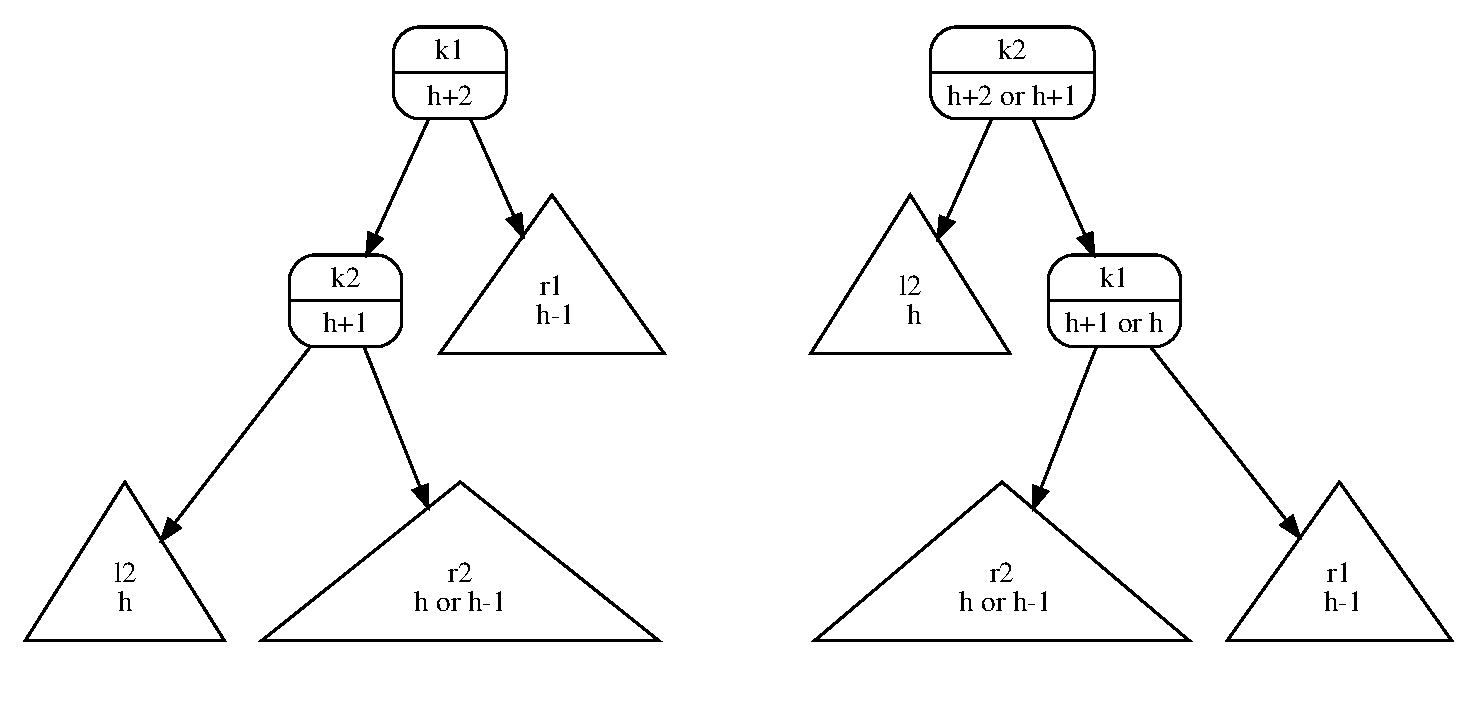
\epsfig{file=Abbildungen/casell.eps,scale=0.63}} 
        \caption{An unbalanced tree and the corresponding rebalanced tree.}
        \label{fig:casell}
      \end{figure}
      We have to make sure that the tree shown in the right part of Figure
      \ref{fig:casell} is indeed an  \textsc{Avl} tree. With respect to the balancing condition this is
      easily verified.  The fact that the node containing the key $k_1$ has either the height
      $h$ or $h+1$ is a consequence of the fact that the height of $r_1$ is  $h-1$ while the height of $r_2$ is
      either $h$ or $h-1$.

      In order to verify that the tree is ordered we can use the following inequation: 
      \\[0.2cm]
      \hspace*{1.3cm}
      $l_2 < k_2 < r_2 < k_1 < r_1$. 
      \hspace*{\fill} $(\star)$
      \\[0.2cm]
      Here we have used the following notation: If  $k$ is a key and  $b$ is a binary tree, then we write \\[0.2cm]
      \hspace*{1.3cm} $k < b$ \\[0.2cm]
      in order to express that  $k$ is smaller than all keys that occur in the tree  $b$.
      Similarly,  $b < k$ denotes the fact that all keys occurring in $b$ are less than the key
      $k$.  The inequation  $(\star)$ describes both the ordering of keys in the left part of Figure
      \ref{fig:casell} and in the right part of this figure.  Hence, the tree shown in the right
      part of Figure \ref{fig:casell} is ordered provided the tree in the left part is ordered to begin with.
\item $\begin{array}[t]{cl}
               & l_1.\mytt{height}() = r_1.\mytt{height}() + 2    \\ 
        \wedge & l_1 = \mytt{Node}(k_2,v_2,l_2,r_2)               \\
        \wedge & l_2.\mytt{height}() < r_2.\mytt{height}()     \\
        \wedge & r_2 = \mytt{Node}(k_3,v_3,l_3,r_3)               \\
        \rightarrow & \mytt{Node}(k_1,v_1,l_1,r_1).\mytt{restore}() = 
                      \mytt{Node}\bigl(k_3,v_3,\mytt{Node}(k_2,v_2,l_2,l_3),\mytt{Node}(k_1,v_1,r_3,r_1) \bigr)
        \end{array}
       $

       The left hand side of this equation is shown in Figure  \ref{fig:caselr} on page
       \pageref{fig:caselr}.  This tree can be written as
       \\[0.2cm]
       \hspace*{1.3cm} 
       $\mytt{Node}\bigl(k_1,v_1,\mytt{Node}(k_2,v_2,l_2,\mytt{Node}\bigl(k_3,v_3,l_3,r_3)\bigr),r_1\bigr)$. 
       \\[0.2cm]
       The subtrees $l_3$ and $r_3$ have either the height  $h$ or $h-1$.  Furthermore, at least one
       of these subtrees must have the height  $h$ for otherwise the subtree
       $\mytt{Node}(k_3,v_3,l_3,r_3)$ would not have the height $h+1$.
       
\begin{figure}[!ht]
  \centering
  \framebox{\epsfig{file=Abbildungen/caselr.eps,scale=0.7}} 
  \caption{An unbalanced tree, second case.}
  \label{fig:caselr}
\end{figure}

     Figure \ref{fig:caselr-nach} on page \pageref{fig:caselr-nach} shows how the tree looks after
     rebalancing.  The tree shown in this figure has the form
     \\[0.2cm]
     \hspace*{1.3cm} 
     $\mytt{Node}\bigl(k_3,v_3,\mytt{Node}(k_2,v_2,l_2,l_3),\mytt{Node}(k_1,v_1,r_3,r_1) \bigr)$.


\begin{figure}[!ht]
  \centering
  \framebox{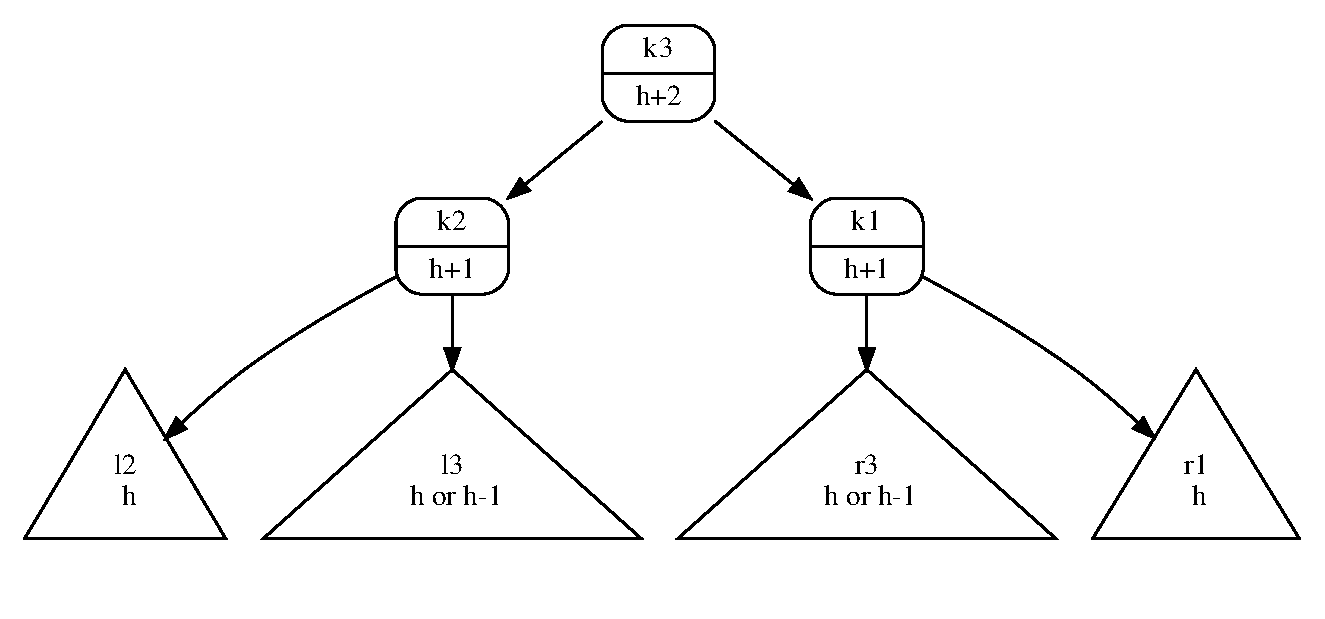
\epsfig{file=Abbildungen/caselr-nach.eps,scale=0.7}} 
  \caption{The rebalanced tree in the second case.}
  \label{fig:caselr-nach}
\end{figure}

      The inequation describing the ordering of the keys both in the tree in Figure \ref{fig:caselr} and the
      tree in Figure \ref{fig:caselr-nach} is given as
      \\[0.2cm]
      \hspace*{1.3cm} $l_2 < k_2 < l_3 < k_3 < r_3 < k_1 < r_1$.

      There are two more cases where the height of the right subtree is bigger by more than 
      the height of the left subtree plus one.  These two cases are completely analogous to the two
      cases discussed previously.  The derivation of the corresponding equations is left as an exercise.
\end{enumerate}

\exercise
Derive the two equations to compute $\mytt{Node}(k_1,v_1,l_1,r_1).\mytt{restore}()$ that have the
precondition $r_1.\mytt{height}() = l_1.\mytt{height}() + 2$.  You should start your derivation of these
equations by drawing diagrams that are analogous to the diagrams shown Figure \ref{fig:casell}, Figure
\ref{fig:caselr}, and Figure \ref{fig:caselr-nach}. 
\eox

Next, we specify the method  $\mytt{insert}()$ via recursive equations.
If we compare these equations to the equations we had given for unbalanced ordered binary trees we
notice that we only have to call the method $\mytt{restore}$ if the balancing condition might have
been violated.
\begin{enumerate}
\item $\mytt{Nil}.\mytt{insert}(k,v) = \mytt{Node}(k,v, \mytt{Nil}, \mytt{Nil})$.  
\item $\mytt{Node}(k, v_2, l, r).\mytt{insert}(k,v_1) = \mytt{Node}(k, v_1, l, r)$.
\item $k_1 < k_2 \rightarrow 
          \mytt{Node}(k_2, v_2, l, r).\mytt{insert}(k_1, v_1) =
          \mytt{Node}\bigl(k_2, v_2, l.\mytt{insert}(k_1,v_1), r\bigr).\mytt{restore}()$.
\item $k_1 > k_2 \rightarrow 
         \mytt{Node}(k_2, v_2, l, r).\mytt{insert}\bigl(k_1, v_1\bigr) = 
         \mytt{Node}\bigl(k_2, v_2, l, r.\mytt{insert}(k_1,v_1)\bigr).\mytt{restore}()$.
\end{enumerate}
The equations for  $\mytt{delMin}()$ change as follows:
\begin{enumerate}
\item $\mytt{Node}(k, v, \mytt{Nil}, r).\mytt{delMin}() = \langle r, k, v \rangle$.
\item $l\not= \mytt{Nil} \wedge \langle l',k_{min}, v_{min}\rangle := l.\mytt{delMin}() 
       \;\rightarrow$ \\[0.2cm]
       \hspace*{1.3cm} 
       $\mytt{Node}(k, v, l, r).\mytt{delMin}() = 
        \langle \mytt{Node}(k, v, l', r).\mytt{restore}(), k_{min}, v_{min} \rangle$.
\end{enumerate}
Finally, the equations for $\mytt{delete}$ are as follows:
\begin{enumerate}
\item $\mytt{Nil}.\mytt{delete}(k) = \mytt{Nil}$.
\item $\mytt{Node}(k,v,\mytt{Nil},r).\mytt{delete}(k) = r$.
\item $\mytt{Node}(k,v,l,\mytt{Nil}).\mytt{delete}(k) = l$.
\item $l \not= \mytt{Nil} \,\wedge\, r \not= \mytt{Nil} \,\wedge\, 
       \langle r',k_{min}, v_{min} \rangle := r.\mytt{delMin}()  \;\rightarrow$ \\[0.2cm]
      \hspace*{1.3cm}
      $\mytt{Node}(k,v,l,r).\mytt{delete}(k) = \mytt{Node}(k_{min},v_{min},l,r').\mytt{restore}()$.
\item $k_1 < k_2 \rightarrow \mytt{Node}(k_2,v_2,l,r).\mytt{delete}(k_1) = 
       \mytt{Node}\bigl(k_2,v_2,l.\mytt{delete}(k_1),r\bigr).\mytt{restore}()$.
\item $k_1 > k_2 \rightarrow \mytt{Node}(k_2,v_2,l,r).\mytt{delete}(k_1) = 
         \mytt{Node}\bigl(k_2,v_2,l,r.\mytt{delete}(k_1)\bigr).\mytt{restore}()$.
\end{enumerate}


\subsection{Implementing AVL-Trees in \textsl{Python}}
If we want to implement \textsc{Avl}-trees in \textsl{Python}, then we have to decide how to compute the height
of the trees.  The idea is to store the height of every subtree in the corresponding node since it
would be inefficient if we would recompute this height every time we need it.  Therefore, we add a
member variable \mytt{mHeight} to our class map.
Figure \ref{fig:avl-tree.ipython:init} shows the constructor of the class \mytt{AvlTree}.  The variable
\mytt{mHeight} is defined in line 7.  It is initialised as $0$ since the constructor \mytt{\_\_init\_\_}
constructs an empty tree.  

\begin{figure}[!ht]
  \centering
\begin{minted}[ frame         = lines, 
                framesep      = 0.3cm, 
                bgcolor       = sepia,
                numbers       = left,
                numbersep     = -0.2cm,
                xleftmargin   = 0.8cm,
                xrightmargin  = 0.8cm
              ]{python3}
    class AvlTree:
        def __init__(self):
            self.mKey    = None
            self.mValue  = None
            self.mLeft   = None
            self.mRight  = None
            self.mHeight = 0 
\end{minted}
\vspace*{-0.3cm}
  \caption{Outline of the class \mytt{map}.}
  \label{fig:avl-tree.ipython:init}
\end{figure}

Figure \ref{fig:avl-tree.ipython:isEmpty} shows the implementation of the function $\mytt{isEmpty}$.
A tree is empty iff its height is $0$.

\begin{figure}[!ht]
\centering
\begin{minted}[ frame         = lines, 
                  framesep      = 0.3cm, 
                  firstnumber   = 1,
                  bgcolor = sepia,
                  numbers       = left,
                  numbersep     = -0.2cm,
                  xleftmargin   = 0.8cm,
                  xrightmargin  = 0.8cm,
                ]{python3}
    def isEmpty(self):
        return self.mHeight == 0
\end{minted}
\vspace*{-0.3cm}
\caption{Implementation of the method $\mytt{isEmpyty}$.}
\label{fig:avl-tree.ipython:isEmpty}
\end{figure}

Figure \ref{fig:avl-tree.ipython:find} shows the implementation of the function $\mytt{find}$.
Actually, this implementation is the same as the implementation that we have given earlier in Figure
\ref{fig:binary-tree.py-1} for ordered binary trees.  The reason is that every \textsc{Avl} tree is also an
ordered binary tree and since searching for a key does not change the underlying tree there is no need to
restore anything. 

\begin{figure}[!ht]
\centering
\begin{minted}[ frame         = lines, 
                  framesep      = 0.3cm, 
                  firstnumber   = 1,
                  bgcolor = sepia,
                  numbers       = left,
                  numbersep     = -0.2cm,
                  xleftmargin   = 0.8cm,
                  xrightmargin  = 0.8cm,
                ]{python3}
    def find(self, key):
        if self.isEmpty():
            return
        elif self.mKey == key:
            return self.mValue
        elif key < self.mKey:
            return self.mLeft.find(key)
        else:
            return self.mRight.find(key)
\end{minted}
\vspace*{-0.3cm}
\caption{Implementation of the method $\mytt{find}$.}
\label{fig:avl-tree.ipython:find}
\end{figure}

Figure \ref{fig:avl-tree.ipython:insert} shows the implementation of the method $\mytt{insert}$.
If we compare this implementation with the implementation for ordered binary trees, we find three
differences.
\begin{enumerate}
\item When inserting into an empty tree, we now have to update the member variable \mytt{mHeight}
      to $1$.  This is done in line 7.
\item After inserting a key-value pair into the left subtree \mytt{mLeft}, it might be necessary to 
      rebalance the tree.  This is done in line 12.
\item Similarly, if we insert a key-value pair into the right subtree \mytt{mRight}, we might have to rebalance 
      the tree.  This is done in line 15.
\end{enumerate}

\begin{figure}[!ht]
\centering
\begin{minted}[ frame         = lines, 
                  framesep      = 0.3cm, 
                  firstnumber   = 1,
                  bgcolor = sepia,
                  numbers       = left,
                  numbersep     = -0.2cm,
                  xleftmargin   = 0.8cm,
                  xrightmargin  = 0.8cm,
                ]{python3}
    def insert(self, key, value):
        if self.isEmpty():
            self.mKey    = key
            self.mValue  = value
            self.mLeft   = AvlTree()
            self.mRight  = AvlTree()
            self.mHeight = 1
        elif self.mKey == key:
            self.mValue = value
        elif key < self.mKey:
            self.mLeft.insert(key, value)
            self._restore()
        else:
            self.mRight.insert(key, value)
            self._restore()
\end{minted}
\vspace*{-0.3cm}
\caption{Implementation of the method $\mytt{insert}$.}
\label{fig:avl-tree.ipython:insert}
\end{figure}

Figure \ref{fig:avl-tree.ipython:delMin} shows the implementation of the method \mytt{delMin}.
The only change compared to the previous implementation for ordered binary trees is in line 7, where
we have to take care of the fact that the balancing condition might be violated after deleting the
smallest element in the left subtree.

\begin{figure}[!ht]
\centering
\begin{minted}[ frame         = lines, 
                framesep      = 0.3cm, 
                firstnumber   = 1,
                bgcolor = sepia,
                numbers       = left,
                numbersep     = -0.2cm,
                xleftmargin   = 0.8cm,
                xrightmargin  = 0.8cm,
              ]{python3}
    def _delMin(self):
        if self.mLeft.isEmpty():
            return self.mRight, self.mKey, self.mValue
        else:
            ls, km, vm = self.mLeft._delMin()
            self.mLeft = ls
            self._restore()
            return self, km, vm
\end{minted}
\vspace*{-0.3cm}
\caption{Implementation of \mytt{delMin}.}
\label{fig:avl-tree.ipython:delMin}
\end{figure}


Figure \ref{fig:avl-tree.ipython:delete} shows the implementation of the method $\mytt{delete}$ and the
implementation of the auxiliary method \mytt{update}.  Compared with Figure
\ref{fig:binary-tree.py-2} there are only three differences:
\begin{enumerate}
\item If we delete the key at the root of the tree, we replace this key with the smallest key in the
      right subtree. Since this key is deleted in the right subtree, the height of the right
      subtree might shrink and hence the balancing condition at the root might be violated.
      Therefore, we have to restore the balancing condition.  This is done in line 11.
\item If we delete a key in the left subtree, the height of the left subtree might shrink.
      Hence we have to rebalance the tree at the root in line 14.
\item Similarly, if we delete a key in the right subtree, we have to restore the balancing
      condition.  This is done in line 17.
\end{enumerate}
Since the method \mytt{update} replaces the current tree with either its left or right subtree and this
subtree is assumed to satisfy the balancing condition, there is no need for a call to \mytt{restore} in this
method. 

\begin{figure}[!ht]
\centering
\begin{minted}[ frame         = lines, 
                framesep      = 0.3cm, 
                firstnumber   = 1,
                bgcolor = sepia,
                numbers       = left,
                numbersep     = -0.2cm,
                xleftmargin   = 0.0cm,
                xrightmargin  = 0.0cm,
              ]{python3}
    def delete(self, key):
        if self.isEmpty():
            return
        if key == self.mKey:
            if self.mLeft.isEmpty():
                self._update(self.mRight)
            elif self.mRight.isEmpty():
                self._update(self.mLeft)
            else:
                self.mRight, self.mKey, self.mValue = self.mRight._delMin()
                self._restore()
        elif key < self.mKey:
            self.mLeft.delete(key)
            self._restore()
        else:
            self.mRight.delete(key)
            self._restore() 

    def _update(self, t):
        self.mKey    = t.mKey
        self.mValue  = t.mValue
        self.mLeft   = t.mLeft
        self.mRight  = t.mRight
        self.mHeight = t.mHeight            
\end{minted}
\vspace*{-0.3cm}
\caption{The methods $\mytt{delete}$ and \mytt{update}.}
\label{fig:avl-tree.ipython:delete}
\end{figure}
\begin{figure}[!ht]
\centering
\begin{minted}[ frame         = lines, 
                framesep      = 0.3cm, 
                firstnumber   = 1,
                bgcolor = sepia,
                numbers       = left,
                numbersep     = -0.2cm,
                xleftmargin   = 0.0cm,
                xrightmargin  = 0.0cm,
              ]{python3}
    def _restore(self):
        if abs(self.mLeft.mHeight - self.mRight.mHeight) <= 1:
            self._restoreHeight()
            return
        if self.mLeft.mHeight > self.mRight.mHeight:
            k1,v1,l1,r1 = self.mKey,self.mValue,self.mLeft,self.mRight
            k2,v2,l2,r2 = l1.mKey, l1.mValue, l1.mLeft, l1.mRight
            if l2.mHeight >= r2.mHeight:
                self._setValues(k2, v2, l2, createNode(k1,v1,r2,r1))
            else: 
                k3,v3,l3,r3 = r2.mKey,r2.mValue,r2.mLeft,r2.mRight
                self._setValues(k3, v3, createNode(k2, v2, l2, l3),
                                        createNode(k1, v1, r3, r1))
        elif self.mRight.mHeight > self.mLeft.mHeight:
            k1,v1,l1,r1 = self.mKey,self.mValue,self.mLeft,self.mRight
            k2,v2,l2,r2 = r1.mKey, r1.mValue, r1.mLeft, r1.mRight
            if r2.mHeight >= l2.mHeight:
                self._setValues(k2, v2, createNode(k1,v1,l1,l2), r2)
            else:
                k3,v3,l3,r3 = l2.mKey,l2.mValue,l2.mLeft,l2.mRight
                self._setValues(k3, v3, createNode(k1, v1, l1, l3),
                                        createNode(k2, v2, r3, r2))
        self._restoreHeight()
    
    def _setValues(self, k, v, l, r):
        self.mKey   = k
        self.mValue = v
        self.mLeft  = l
        self.mRight = r
    
    def _restoreHeight(self):
        self.mHeight = max(self.mLeft.mHeight, self.mRight.mHeight) + 1
\end{minted}
\vspace*{-0.3cm}
\caption{The implementation of \mytt{restore} and \mytt{restoreHeight}.}
\label{fig:avl-tree.ipython:restore}
\end{figure}


Figure \ref{fig:avl-tree.ipython:restore} shows the implementation of the function \mytt{restore}.
It is this method that makes most of the difference between ordered binary trees and \textsc{Avl} trees.  Let
us discuss this method line by line.
\begin{enumerate}
\item In line 2 we check whether the balancing condition is satisfied.  If we are lucky,  this test 
      is successful and hence we do not need to restore the structure of the tree.  However, we
      still need to maintain the height of the tree since it is possible that the variable
      \mytt{mHeight} no longer contains the correct height.  For example, assume that the left subtree
      initially has a height that is bigger by one than the height of the right subtree.  Assume
      further that we have deleted a node in the left subtree so that its height shrinks.  Then the
      balancing condition is still satisfied, as now the left subtree and the right subtree have the
      same height.  However, the height of the complete tree has also shrunk by one and therefore, 
      the variable \mytt{mHeight} needs to be decremented.  This is done via the auxiliary method
      \mytt{restoreHeight}.  This method is defined in line 31 and it recomputes \mytt{mHeight}
      according to the definition of the height of a binary tree.
\item If the check in line 2 fails, then we know that the balancing condition is violated.
      However, we do not yet know which of the two subtrees is bigger.  

      If the test in line 5 succeeds, then the left subtree must have a height that is bigger by
      two than the height of the right subtree.  In order to be able to use the same variable names 
      as the variable names given in the equations discussed in the previous subsection, we define
      the variables \mytt{k1}, \mytt{v1}, \mytt{l1}, \mytt{r1}, \mytt{k2}, \mytt{v2}, \mytt{l2},
      and \mytt{r2} in line 6 and 7 so that these variable names correspond exactly to the variable names
      used in the Figures \ref{fig:casell} and \ref{fig:caselr}.
\item Next, the test in line 8 checks whether we have the case that is depicted in Figure
      \ref{fig:casell}.  In this case, Figure \ref{fig:casell} tells us that the key \mytt{k2}
      has to move to the root.  The left subtree is now \mytt{l2}, while the right subtree is a
      new node that has the key \mytt{k1} at its root.  This new node is created by the call
      of the function \mytt{createNode} in line 9.  The function \mytt{createNode} is shown in
      Figure \ref{fig:avl-tree.ipython:createNode} on page \pageref{fig:avl-tree.ipython:createNode}.
\item If the test in line 8 fails, the right subtree is bigger than the left subtree and we are in 
      the case that is depicted in Figure \ref{fig:caselr}.  We have to create the tree that is
      shown in Figure \ref{fig:caselr-nach}.  To this end we first define the variables 
      \mytt{k3}, \mytt{v3}, \mytt{l3}, and \mytt{r3} in a way that these variables
      correspond to the variables shown in Figure \ref{fig:caselr}.  Next, we create the tree
      that is shown in Figure \ref{fig:caselr-nach}.
\item Line 14 deals with the case that the right subtree is bigger than the left subtree. 
      As this case is analogous to the case covered in line 5 to line 13, we won't discuss this case
      any further.
\item Finally, we recompute the variable \mytt{mHeight} since it is possible that the old value is
      no longer correct.
\end{enumerate}


\begin{figure}[!ht]
\centering
\begin{minted}[ frame         = lines, 
                framesep      = 0.3cm, 
                firstnumber   = 1,
                bgcolor = sepia,
                numbers       = left,
                numbersep     = -0.2cm,
                xleftmargin   = 0.8cm,
                xrightmargin  = 0.8cm,
              ]{python3}
    def createNode(key, value, left, right):
        node         = AvlTree()
        node.mKey    = key
        node.mValue  = value
        node.mLeft   = left
        node.mRight  = right
        node.mHeight = max(left.mHeight, right.mHeight) + 1
        return node
\end{minted}
\vspace*{-0.3cm}
\caption{Implementation of \mytt{createNode}.}
\label{fig:avl-tree.ipython:createNode}
\end{figure}

The function \mytt{createNode} shown in Figure \ref{fig:avl-tree.ipython:createNode}
constructs a node with given left and right subtrees.  In fact, this method serves as a second
constructor for the class \mytt{map}.  The implementation should be obvious.


\subsection{Analysis of the Complexity of AVL Trees}
Next, we analyse the complexity of \textsc{Avl} trees in the worst case.  In order to do this we have to know
what the worst case actually looks like.  Back when we only had ordered binary trees the worst case was the case where
the tree had degenerated into a list.  Now, the worst case is the case where the tree is as slim as
it can possibly be while still satisfying the balancing condition of an \textsc{Avl} tree.  Hence the worst case
happens if the tree has a given height $h$ but the number of keys stored in the tree is as small as
possible.  To investigate trees of this kind, let us define  $b_h(k)$ as an \textsc{Avl} tree that has the following three
properties:
\begin{enumerate}[(a)]
\item The height of $b_h(k)$ is $h$.
\item The number of keys stored in $b_h(k)$ is minimal among all other \textsc{Avl} trees of height $h$.  
\item All keys stored in  $b_h(k)$ are natural number that are bigger than  $k$.

      In order for the expression $b_h(k)$ to be unambiguously defined we demand that the keys
      in $b_h(k)$ are natural numbers that are as small as possible.  Furthermore, as the values do
      not really matter, we define the values to be $0$.
\item If $h > 1$, then the height of the left subtree of $b_h(k)$ is bigger than the height of its right subtree.
\end{enumerate}
For our investigation of the complexity, both the keys and the values do not really matter.  The only problem
is that we have to ensure that the tree $b_h(k)$ is an ordered tree.
Before we can present the definition of $b_h(k)$ we need to define the auxiliary function
$\mytt{maxKey}()$, which computes the largest key that is stored in a given tree.  This function has the
 signature  
\\[0.2cm]
\hspace*{1.3cm}
$\mytt{maxKey}:\mathcal{B} \rightarrow \mytt{Key} \cup \{ \Omega \}$.
\\[0.2cm]
Given an ordered binary tree  $b$, the expression $b.\mytt{maxKey}()$ returns the largest
key that is stored in $b$.  The expression  $b.\mytt{maxKey}()$ is defined by induction on $b$:
\begin{enumerate}
\item $\mytt{Nil}.\mytt{maxKey}() = \Omega$,
\item $\mytt{Node}(k,v,l,\mytt{Nil}).\mytt{maxKey}() = k$,
\item $r \not= \mytt{Nil} \rightarrow \mytt{Node}(k,v,l,r).\mytt{maxKey}() = r.\mytt{maxKey}()$.
\end{enumerate}
Now we are ready to define the tree $b_h(k)$ by induction on  $h$.
\begin{enumerate}
\item $b_0(k) = \mytt{Nil}$,

      because there is only one \textsc{Avl} tree of height $0$ and this is the tree $\mytt{Nil}$.
\item $b_1(k) = \mytt{Node}(k+1,0,\mytt{Nil}, \mytt{Nil})$,

      since, if we abstract from the actual keys and values, there is exactly one \textsc{Avl} tree of height
      $1$.
\item $b_{h+1}(k).\mytt{maxKey}() = l \rightarrow 
       b_{h+2}(k) = \mytt{Node}\bigl(l+1,\,0,\,b_{h+1}(k),\,b_h(l+1)\bigr)$.

      In order to construct an \textsc{Avl} tree of height $h+2$ that contains the minimal number of keys 
      we first construct the \textsc{Avl} tree $b_{h+1}(k)$ which has height  $h+1$ and which stores as few
      key as possible given its height.  Next, we determine the biggest key $l$ in this tree. 
      Now to construct $b_{h+2}(k)$ we take a node with the key $l+1$ as the root.
      The left subtree $b_{h+2}(k)$ is $b_{h+1}(k)$, while its right subtree is $b_h(l+1)$.
      Since $l$ is the biggest key in $b_{h+1}(k)$, all key in the left subtree of
      $b_{h+2}(k)$ are indeed smaller than the key $l+1$ at the root.  Since all keys in
      $b_h(l+1)$ are bigger than $l+1$, the keys in the right subtree are bigger than the key at the
      root.  Therefore, $b_{h+2}(k)$ is an \textsc{Avl} tree.

      Furthermore, $b_{h+2}(k)$ is an \textsc{Avl} tree of height $h+2$ since the height of the left subtree
      is $h+1$ and the height of the right subtree is $h$.  Also, this tree is as slim as
      any \textsc{Avl} tree can possibly get, since if the left subtree has height $h+1$ the right subtree
      must at least have height $h$ in order for the whole tree to satisfy the balancing condition.
\end{enumerate}
Let us denote the number of keys stored in a binary tree $b$ as  $\#\,b$.  We define
\\[0.2cm]
\hspace*{1.3cm}
$c_h := \#\, b_h(k)$
\\[0.2cm]
to be the number of keys in the tree $b_h(k)$.  An easy induction on $h$ shows that 
$\#\,b_h(k)$ does not depend on the number $k$ and therefore $c_h$ does not depend on $k$.  Starting
from the definition of $b_h(k)$ we find the following equations for $c_h$:
\begin{enumerate}
\item $c_0 = \#\, b_0(k) = \#\, \mytt{Nil} = 0$,
\item $c_1 = \#\, b_1(k) = \#\, \mytt{Node}(k+1,0,\mytt{Nil}, \mytt{Nil}) = 1$, 
\item$\begin{array}[t]{lcl}
       c_{h+2} & = & \#\, b_{h+2}(k) \\
               & = & \#\,\mytt{Node}\bigl(l+1,\,0,\,b_{h+1}(k),\,b_h(l+1)\bigr) \\
               & = & \#\, b_{h+1}(k) + \#\, b_h(l+1) + 1 \\
               & = & c_{h+1} + c_h + 1.
       \end{array}$
\end{enumerate}
Hence we have found the \href{https://en.wikipedia.org/wiki/Recurrence_relation}{recurrence equation}
\\[0.2cm]
\hspace*{1.3cm}
$c_{h+2} = c_{h+1} + c_h + 1 \quad \mbox{with initial values $c_0 = 0$ and $c_1 = 1$}.$
\\[0.2cm]
This also validates our claim that $c_h$ does not depend on $k$.  This is a linear, inhomogeneous recurrence
equation.  In order to solve this recurrence
equation we first solve the corresponding \blue{homogeneous recurrence equation} 
\\[0.2cm]
\hspace*{1.3cm}
$a_{h+2} = a_{h+1} + a_h$
\\[0.2cm]
using the \href{https://en.wikipedia.org/wiki/Ansatz}{ansatz}
\\[0.2cm]
\hspace*{1.3cm}
$a_h = \lambda^h$.
\\[0.2cm]
Substituting $a_h = \lambda^h$ into the recurrence equation for $a_h$ leaves us with the equation
\\[0.2cm]
\hspace*{1.3cm}
$\lambda^{h+2} = \lambda^{h+1} + \lambda^{h}$.
\\[0.2cm]
Dividing by $\lambda^h$ leaves the quadratic equation
\\[0.2cm]
\hspace*{1.3cm}
$\lambda^2 = \lambda + 1$
\\[0.2cm]
which can be rearranged as
\\[0.2cm]
\hspace*{1.3cm}
$\ds \lambda^2 - 2 \cdot \lambda \cdot \frac{1}{2} = 1$.
\\[0.2cm]
To complete the square we add $\bigl(\frac{1}{2}\bigr)^2$ on both sides of this equation:
\\[0.2cm]
\hspace*{1.3cm}
$\ds \lambda^2 - 2 \cdot \lambda \cdot \frac{1}{2} + \Bigl(\frac{1}{2}\Bigr)^2 = 1 + \frac{1}{4}$.
\\[0.2cm]
This is equivalent to
\\[0.2cm]
\hspace*{1.3cm}
$\ds \Bigl(\lambda - \frac{1}{2}\Bigr)^2 = \frac{5}{4}$. 
\\[0.2cm]
From this we conclude 
\\[0.2cm]
\hspace*{1.3cm}
$\ds\lambda = \frac{1}{2} \cdot \bigl(1 + \sqrt{5}\bigr) \;\vee\; \lambda = \frac{1}{2} \cdot \bigl(1 - \sqrt{5}\bigr)$.
\\[0.2cm]
Let us therefore define 
\\[0.2cm]
\hspace*{1.3cm}
$\ds\lambda_1 =  \frac{1}{2} \cdot \bigl(1 + \sqrt{5}\bigr) \approx  1.618034$ \quad and \quad 
$\ds\lambda_2 = \frac{1}{2} \cdot \bigl(1 - \sqrt{5}\bigr) \approx -0.618034$.
\\[0.2cm]
In order to solve the \blue{inhomogeneous recurrence equation} for $c_h$ we try the ansatz
\\[0.2cm]
\hspace*{1.3cm}
$c_h = d$ \quad for some constant $d$.
\\[0.2cm]
Substituting this ansatz into the recurrence equation for $c_h$ yields
\\[0.2cm]
\hspace*{1.3cm}
$d = d + d + 1$,
\\[0.2cm]
from which we conclude that $d = -1$.  The solution for $c_h$ is now a linear combination of the solutions for
the corresponding homogeneous recurrence equation to which we have to add the solution for the inhomogeneous equation:
\\[0.2cm]
\hspace*{1.3cm}
$c_h = \alpha \cdot \lambda_1^h + \beta \cdot \lambda_2^h + d =\alpha \cdot \lambda_1^h + \beta \cdot \lambda_2^h - 1$.
\\[0.2cm]
Here, the values of $\alpha$ and $\beta$ can be found by setting $h=0$ and $h=1$ and using the
initial conditions $c_0 = 0$ and $c_1 = 1$.  This results in
the following system of linear equations for  $\alpha$ and $\beta$:
\\[0.2cm]
\hspace*{1.3cm}
$0 = \alpha + \beta - 1$ \quad and \quad
$1 = \alpha \cdot \lambda_1 + \beta \cdot \lambda_2 - 1$.
\\[0.2cm]
From the first equation we find $\beta = 1-\alpha$ and substituting this result into the second equation
gives
\\[0.2cm]
\hspace*{1.3cm}
$2 = \alpha \cdot \lambda_1 + (1-\alpha) \cdot \lambda_2$.
\\[0.2cm]
Solving this equation for $\alpha$ gives
\\[0.2cm]
\hspace*{1.3cm}
$2 - \lambda_2 = \alpha \cdot (\lambda_1 - \lambda_2)$
\\[0.2cm]
and therefore
\\[0.2cm]
\hspace*{1.3cm}
$\ds \alpha = \frac{2 - \lambda_2}{\lambda_1 - \lambda_2}$.
\\[0.2cm]
Now it just so happens that $\lambda_1 - \lambda_2 = \sqrt{5}$ and, furthermore, $2 - \lambda_2 = \lambda_1^2$.
We prove only the second claim, since the first is easy to verify.  We have the following
chain of equivalences:
$$
\begin{array}{crcl}
                  & 2 - \lambda_2 & = & \lambda_1^2            \\[0.2cm]
  \Leftrightarrow & 2 - \lambda_2 & = & \lambda_1 + 1          \\[0.2cm]
  \Leftrightarrow & 1             & = & \lambda_1 + \lambda_2  \\[0.2cm]
  \Leftrightarrow & 1             & = &\frac{1}{2} \cdot (1 + \sqrt{5}) + \frac{1}{2} \cdot (1 - \sqrt{5}) 
\end{array}
$$
Since the last equation is obviously true, the first is also true.
Hence, we have found
\\[0.2cm]
\hspace*{1.3cm}
$\ds \alpha = \frac{2 - \lambda_2}{\lambda_1 - \lambda_2} = \frac{1}{\sqrt{5}} \cdot \lambda_1^2$.
\\[0.2cm]
From this, a straightforward calculation using the fact that $\beta = 1 - \alpha$ shows that 
\\[0.2cm]
\hspace*{1.3cm}
$\ds \beta  = -\frac{1}{\sqrt{5}} \cdot \lambda_2^2$.
\\[0.2cm]
Therefore, $c_h$ is given by the following equation:
\\[0.2cm]
\hspace*{1.3cm}
$c_h = \ds \frac{1}{\sqrt{5}} \cdot \left( \lambda_1^{h+2} - \lambda_2^{h+2} \right) -1$.  
\\[0.2cm]
As we have  $|\lambda_2| < 1$, the value of  $\ds\lambda_2^{h+2}$ isn't important for big
values of $h$.  Therefore, for big values of $h$, the minimal number  $n$ of keys in a tree of
height  $h$ is approximately given by the formula \\[0.2cm]
\hspace*{1.3cm} $n \approx \ds \frac{1}{\sqrt{5}} \cdot \lambda_1^{h+2} - 1$. \\[0.2cm]
In order to solve this equation for  $h$ we take the logarithm of both side.  Then we have
\\[0.2cm]
\hspace*{1.3cm}
$\log_2(n+1) = (h+2) \cdot \log_2(\lambda_1) - \frac{1}{2}\cdot \log_2(5)$.
\\[0.2cm]
Adding  $\frac{1}{2}\cdot \log_2(5)$ gives
\\[0.2cm]
\hspace*{1.3cm}
$\log_2(n+1) + \frac{1}{2}\cdot \log_2(5) = (h+2) \cdot \log_2(\lambda_1)$.
\\[0.2cm]
Let us divide this inequation by  $\log_2(\lambda_1)$.  Then we get
\\[0.4cm]
\hspace*{1.3cm}
$\ds \bruch{\log_2(n+1) + \frac{1}{2}\cdot \log_2(5)}{\log_2(\lambda_1)} = h+2$.
\\[0.2cm]
Solving this equation for  $h$ yields the result 
\\[0.4cm]
\hspace*{1.3cm} 
$
\begin{array}[t]{lcl}
h & = & \ds \frac{\log_2(n+1) + \frac{1}{2}\cdot \log_2(5)}{\log_2(\lambda_1)} - 2 \\[0.4cm]
  & = & \ds \frac{1}{\log_2(\lambda_1)}\cdot \log_2(n) + \Oh(1) \\[0.5cm]
  & \approx & 1,44 \cdot \log_2(n) + \Oh(1).
\end{array} 
$
\\[0.2cm]
Above we have used the fact that 
\\[0.2cm]
\hspace*{1.3cm}
$\log_2(n+1) - \log_2(n) \in \Oh(1)$. 
\\[0.2cm]
As the height $h$ is the maximal number of comparisons needed to find a given key
the complexity of $b.\mytt{find}(k)$ for an \textsc{Avl} tree $b$ is logarithmic even in the worst case.
Figure 
\ref{fig:avl-worst-case} presents an  \textsc{Avl} tree of height 6 where the number of keys is minimal.



\begin{figure}[!ht]
  \centering
  \framebox{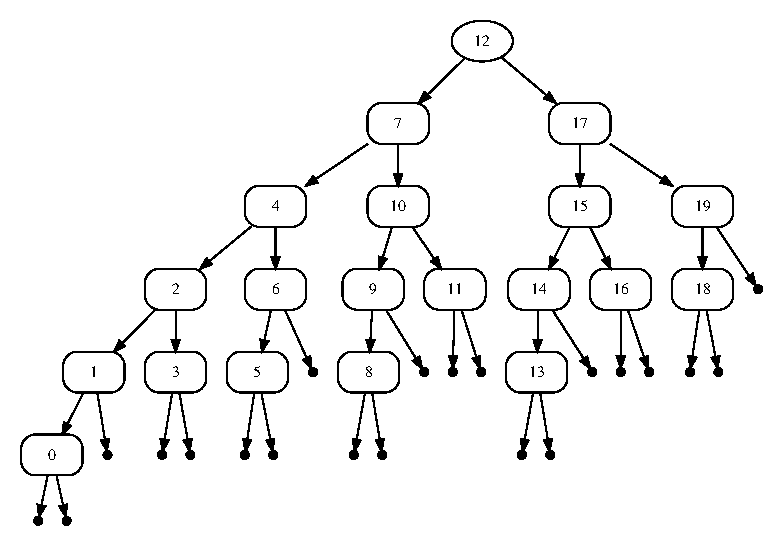
\epsfig{file=Abbildungen/avl}} 
  \caption{An \textsc{Avl} tree of height 6 that is as slim as possible. Values are not shown.}
  \label{fig:avl-worst-case}
\end{figure}

\subsection{Improvements}
In practice, 
\href{https://en.wikipedia.org/wiki/Red-black_trees}{red-black trees} \index{red-black tree}
are slightly faster than \textsc{\textsc{Avl}} trees.  Similar to
\textsc{\textsc{Avl}} trees, a  red-black tree
  is an ordered binary tree that is approximately balanced.  Nodes are either black or red.
The children of a red node have to be black.  In order to keep red-black trees approximately
balanced, a \blue{relaxed height} of a tree is defined.  Red nodes do not contribute to the relaxed
height of a tree.  The left and right subtree of every node of a red-black tree are required to have the same 
relaxed height.  A detailed and very readable exposition of red-black trees is given by Sedgewick
\cite{sedgewick:2011}.  Red-black trees have been invented by Leonidas L.~Guibas and 
\href{https://en.wikipedia.org/wiki/Robert_Sedgewick_(computer_scientist)}{Robert Sedgewick} \cite{guibas:78}.

\exercise
Instead of using \textsc{Avl} trees, another alternative to implement a map is to use 
\href{https://en.wikipedia.org/wiki/2-3_tree}{2-3 trees}.  \index{2-3 tree}
Below we describe a simplified version of these trees.  These trees do not store any values.  Hence, instead
of implementing maps, these trees implement sets. They are built using the following constructors:
\begin{enumerate}
\item $\mytt{Nil}$ is a 2-3 tree that represents the empty set.
\item $\mytt{Two}(l, k, r)$ is a 2-3 tree provided
      \begin{enumerate}[(a)]
      \item $l$ is a 2-3 tree,
      \item $k$ is a key,
      \item $r$ is a 2-3 tree,
      \item all keys stored in $l$ are less than k and all keys stored in $r$ are bigger than $k$,
            i.e.~we have
            \\[0.2cm]
            \hspace*{1.3cm}
            $l < k < r$.
      \item $l$ and $r$ have the same height.
      \end{enumerate}
      A node of the form  $\mytt{Two}(l, k, r)$ is called a \blue{2-node}.  Except for the fact
      that there is no value, a 2-node is
      interpreted in the same way as we have interpreted the term $\mytt{Node}(k, v, l, r)$.
\item $\mytt{Three}(l, k_1, m, k_2, r)$ is a 2-3 tree provided
      \begin{enumerate}[(a)]
      \item $l$, $m$, and $r$ are 2-3 trees,
      \item $k_1$ and $k_2$ are keys,
      \item $l < k_1 < m < k_2 < r$,
      \item $l$, $m$, and $r$ have the same height.
      \end{enumerate}
      A node of the form  $\mytt{Three}(l, k_1, m, k_2, r)$ is called a \blue{3-node}.
\end{enumerate}
In order to keep 2-3 trees balanced when inserting new keys, we use a fourth constructor of the form
\\[0.2cm]
\hspace*{1.3cm}
$\mytt{Four}(l,k_1,m_l, k_2, m_r, k_3, r)$.
\\[0.2cm]
A term of the form $\mytt{Four}(l,k_1,m_l, k_2, m_r, k_3, r)$ is a \blue{2-3-4} tree iff
\begin{enumerate}
\item $l$, $m_l$, $m_r$, and $r$ are 2-3 trees,
\item $k_1$, $k_2$, and $k_3$ are keys,
\item $l < k_1 < m_l < k_2 < m_r < k_3 < r$,
\item $l$, $m_l$, $m_r$, and $r$ all have the same height.
\end{enumerate}
Nodes of this form are called 4-nodes and the key $k_2$ is called the \blue{middle key}.
Trees containing 4-nodes are called \blue{2-3-4} trees.
When a new key is inserted into a 2-3 tree, the challenge is to keep the tree balanced.  The easiest
case is the case where the tree has the form
\\[0.2cm]
\hspace*{1.3cm}
$\mytt{Two}(\mytt{Nil}, k, \mytt{Nil})$.
\\[0.2cm]
In this case, the 2-node is converted into a 3-node.  If the tree has the form 
\\[0.2cm]
\hspace*{1.3cm}
$\mytt{Three}(\mytt{Nil}, k_1, \mytt{Nil}, k_2, \mytt{Nil})$,
\\[0.2cm]
the 3-node is temporarily transformed into a 4-node.  Next, the middle key of this node is lifted up
to its parent node.  For example, suppose we insert the key 3 into the tree
\\[0.2cm]
\hspace*{1.3cm}
$\mytt{Two}(\mytt{Two}(\mytt{Nil}, 1, \mytt{Nil}), 2, \mytt{Three}(\mytt{Nil}, 4, \mytt{Nil}, 5, \mytt{Nil}))$.
\\[0.2cm]
In this case, the key 3 needs to be inserted to the left of the key 4.  This yields the temporary tree 
\\[0.2cm]
\hspace*{1.3cm}
$\mytt{Two}(\mytt{Two}(\mytt{Nil}, 1, \mytt{Nil}), 2, \mytt{Four}(\mytt{Nil}, 3, \mytt{Nil}, 4, \mytt{Nil}, 5, \mytt{Nil}))$,
\\[0.2cm]
where the right subtree is the 4-node $\mytt{Four}(\mytt{Nil}, 3, \mytt{Nil}, 4, \mytt{Nil}, 5, \mytt{Nil})$.
Since this is not a 2-3 tree, we need to lift the middle key 4 to its parent node.  This results in
the new tree
\\[0.2cm]
\hspace*{1.3cm}
$\mytt{Three}(\mytt{Two}(\mytt{Nil}, 1, \mytt{Nil}), 2, \mytt{Two}(\mytt{Nil}, 3, \mytt{Nil}), 4, \mytt{Two}(\mytt{Nil}, 5, \mytt{Nil}))$.
\\[0.2cm]
This tree is a 2-3 tree.  In this example we have been lucky since the parent of the 4-node was
a 2 node and therefore we could transform it into a 3-node.  If the parent node instead is a 3-node,
it has to be transformed into a temporary 4-node.  Then, the middle key of this 4-node has to be
lifted up recursively to its parent.  
\begin{enumerate}[(a)]
\item Specify a method $t.\mytt{member}(k)$ that checks whether the key $k$ occurs in the 2-3 tree
      $t$.  You should use recursive equations to specify  $t.\mytt{member}(k)$.
\item Specify a method $t.\mytt{insert}(k)$ that inserts the key $k$ into the 2-3 tree
      $t$.  You should use three auxiliary functions to implement \mytt{insert}:
      \begin{enumerate}
      \item $t.\mytt{ins}(k)$ takes a 2-3 tree $t$ and a key $k$ and inserts the key $k$ into $t$.
            It returns a 2-3-4 tree that has at most one 4-node.  Unless the tree $t$ has a height of $1$, this
            4-node has to be a child of the root node.  The function \mytt{ins} is recursive and uses the
            function \mytt{restore} that is described next.
            Furthermore, the height of the tree $t.\mytt{ins}(k)$ has to be the same as the height of the tree $t$.
      \item $t.\mytt{restore}()$ takes a 2-3-4 tree $t$ that has at most one 4-node, which has to be a child
            of the root.  It returns a 2-3-4 tree that has at most one 4-node.  This 4-node has to be the root node.
            Furthermore, the height of the tree $t.\mytt{restore}()$ has to be the same as the height of the tree $t$.
      \item $t.\mytt{grow}()$ takes a 2-3-4 tree $t$ that has at most one 4-node, which has to be the root
            node of the tree.  It returns an equivalent 2-3 tree.  The height of this tree is either the same
            as the height of $t$ or it is the height of $t$ plus $1$.
      \end{enumerate}
      Having defined these auxiliary functions, the function \mytt{insert} can then be computed as follows:
      \\[0.2cm]
      \hspace*{1.3cm}
      $t.\mytt{insert}(k) = t.\mytt{ins}(k).\mytt{restore}().\mytt{grow}()$.
\item Implement 2-3 trees in \textsl{Python}.
\item \textbf{Optional}: Specify a method $t.\mytt{delete}(k)$ that deletes the key $k$ in the tree $t$.

      In order to implement the function \mytt{delete}, it is necessary to define 1-2-3 trees.
      In addition to both 2-nodes and 3-nodes, these trees also have 1-nodes.  These nodes come into existence
      when a key is deleted from a 2-node:  Deleting the key $k$ from the node
      \\[0.2cm]
      \hspace*{1.3cm}
      $\mytt{Two}(\mytt{Nil}, k, \mytt{Nil})$
      \\[0.2cm]
      creates the 1-node $\mytt{One}(\mytt{Nil})$.
\end{enumerate}
Prof. Lyn Turbak has written a helpful
\href{http://www.cs.princeton.edu/~dpw/courses/cos326-12/ass/2-3-trees.pdf}{paper} describing 2-3 trees in more
depth.  This paper gives a graphical presentation of the \mytt{insert} and \mytt{delete} operations.

\paragraph{History:}
According to \cite{cormen:09}, 2-3 trees have been invented by
\href{https://en.wikipedia.org/wiki/John_Hopcroft}{John Hopcroft} in 1970.  John Hopcroft received the 1986
Turing Award. 



\section{Tries}
Often, the keys of a map are strings.  For example, when you search with 
\href{https://www.google.com}{\blue{G}\red{o}\orange{o}\blue{g}\green{l}\red{e}}, you are using
a string as a key to lookup information that is stored in a gigantic map provided by Google.
As another example, in an electronic phone book the keys are names and therefore strings.  
There is a species of search trees that is particularly well adapted to the case that the keys are
strings.  These search trees are known as \href{https://en.wikipedia.org/?title=Trie}{tries}.  
The name is derived from the word
\blue{re\underline{trie}val}.  In order to be able to distinguish between \blue{tries} and
\blue{trees} we have to pronounce  \blue{trie}  so that it rhymes with \blue{pie}.   The data
structure of tries has been proposed 1959 by Ren\'e de la Briandais \cite{briandais:59}.

Tries are also trees, but in contrast to a binary tree where every node has two children, in a trie a
node can have as many children as there are characters in the alphabet that is used to represent the
strings.  In order to define tries formally we assume that the following is given:
\begin{itemize}
\item $\Sigma$ is finite set of \blue{characters}. $\Sigma$ is called the
      \blue{alphabet}. 
\item $\Sigma^*$ is the set of all \blue{strings} that are built from the characters of $\Sigma$.
      Formally, a string is just a list of characters.  If we have $w \in \Sigma^*$, then we write $w = cr$
      if $c$ is the first character of $w$ and if $r$ the string that remains if we remove the first
      character from $w$.
\item $\varepsilon$ denotes the empty string.
\item $\mytt{Value}$ is the set of all the values that can be associated with the keys.  
\end{itemize}
The set $\mathbb{T}$ of all tries \index{trie} is defined inductively using the constructor \\[0.2cm]
\hspace*{1.3cm} 
$\mytt{Trie}: \mytt{Value} \times \mytt{List}(\Sigma) \times
\mytt{List}(\mathbb{T}) \rightarrow \mathbb{T}$. 
\\[0.2cm]
The inductive definition of the set $\mathbb{T}$ \index{$\mathbb{T}$} has only a single clause: If
\begin{enumerate}[(a)]
\item $v \in \mytt{Value} \cup \{\Omega\}$,
\item $C\!s = [c_1, \cdots, c_n] \in \mytt{List}(\Sigma)$ is a list of different characters of length
      $n$ and,
\item $T\!s = [t_1, \cdots, t_n] \in \mytt{List}(\mathbb{T})$ is a list of  tries of the same length $n$, 
\end{enumerate}
then we have 
\\[0.2cm]
\hspace*{1.3cm}  $\mytt{Trie}(v, C\!s, T\!s) \in \mathbb{T}$.  
\\[0.2cm]
As there is only one clause in this definition, you might ask how this inductive definition gets started.
The answer is that the base case of this inductive definition is the case where
$n=0$ since in that case the lists  $C\!s$ and $T\!s$ are both empty.  Therefore, the empty trie has the form
\\[0.2cm]
\hspace*{1.3cm}
$\mytt{Trie}(\Omega, [], [])$.
\\[0.2cm]
In order to specify the semantics of a trie of the form $\mytt{Trie}(v,C,T)$ 
we specify a function
\\[0.2cm]
\hspace*{1.3cm} 
$\mytt{find}: \mathbb{T} \times \Sigma^* \rightarrow \mytt{Value} \cup \{ \Omega\}$
\\[0.2cm]
that takes a trie $t$ and a string $s$ as its arguments.  The expression $t.\mytt{find}(s)$ returns the
value that is associated with the key $s$ in $t$.  The value of the expression
$t.\mytt{find}(s)$ is defined by induction on the length of the  string $s$:
\begin{enumerate}
\item $\mytt{Trie}(v, C\!s, T\!s).\mytt{find}(\varepsilon) = v$.

      The value associated with the empty string $\varepsilon$ is stored at the root of the trie.
\item $c = c_i \rightarrow 
       \mytt{Trie}(v, [c_1, \cdots, c_n], [t_1, \cdots, t_n]).\mytt{find}(cr) = t_i.\mytt{find}(r)
      $

      The trie $\mytt{Trie}(v, [c_1, \cdots, c_n], [t_1, \cdots, t_n])$ associates a value with
      the key $cr$ if the list $[c_1, \cdots, c_n]$ has a position $i$ such that $c$ equals $c_i$
      and, furthermore, the trie  $t_i$ associates a value with the key  $r$.
\item $ c \not\in C\!s \rightarrow
       \mytt{Trie}(v, C\!s, T\!s).\mytt{find}(cr) = \Omega
      $

      If $c$ does not occur in the list $C\!s$, then the trie $\mytt{Trie}(v, C\!s, T\!s)$ does not store a value for
      the key $cr$.
\end{enumerate}

\begin{figure}[!ht]
  \centering
  \framebox{\epsfig{file=Abbildungen/trie}} 
  \caption{A trie storing some arbitrary numbers.}
  \label{fig:trie}
\end{figure}

Graphically, tries are represented as trees.  Since it would be unwieldy to label the nodes of these
trees with the lists of characters corresponding to these nodes, we use a trick:  In order to
visualize a node of the form \\[0.2cm]
\hspace*{1.3cm} 
$\mytt{Trie}(v, [c_1, \cdots, c_n], [t_1, \cdots, t_n])$ \\[0.2cm]
we draw a rectangle with rounded corners.  This rectangle is split into two parts by a horizontal line.
If the value  $v$ that is stored in this node is different from $\Omega$, then $v$ is
written in the lower part of the rectangle.  The label that we put in the upper half of the rectangle
depends on the parent of the node.  We will explain how this label is computed in a moment.
The node itself has $n$ different children.  These $n$ children are the tries
$t_1$, $\cdots$, $t_n$.  The node at the root of the trie $t_i$ is labelled with the character $c_i$,
i.e.~the rectangle that represents this node carries the label $c_i$ in its upper half.

In order to clarify these ideas, Figure  \ref{fig:trie} on page \pageref{fig:trie} shows a trie
mapping some strings to numbers.  The mapping depicted in this tree can be written as a \textsl{Python}
dictionary: 
\\[0.2cm]
\hspace*{1.3cm} $ \bigl\{ \mytt{'Stahl'}: 1, \mytt{'Stolz'}: 2, \mytt{'Stoeger'}: 3, \mytt{'Salz'}: 4, \mytt{'Schulz'}: 5$, \\[0.2cm]
\hspace*{1.5cm} $         \mytt{'Schulze'}: 6, \mytt{'Schnaut'}: 7, \mytt{'Schnupp'}: 8, \mytt{'Schroer'}: 9\bigr\}$. \\[0.2cm]
Since the node at the root has no parent, the upper half of  the rectangle representing the root is
always empty.  In the example shown in Figure \ref{fig:trie}, the lower half of this rectangle is also empty
because the trie doesn't associate a value with the empty string.  In this example, the root node corresponds
to the term  
\\[0.2cm]
\hspace*{1.3cm}
 $\mytt{Trie}(\Omega,[\mytt{'S'}], [t])$. 
\\[0.2cm]
Here,  $t$ denotes the trie that is labelled with the character  \mytt{'S'} at its root.
This trie can then be represented by the term  \\[0.2cm]
\hspace*{1.3cm} 
$\mytt{Trie}(\Omega,[\mytt{'t'},\mytt{'a'},\mytt{'c'}], [t_1, t_2, t_3])$. \\[0.2cm]
This trie has three children that are labelled with the characters  \mytt{'t'}, \mytt{'a'}, and \mytt{'c'}.

\subsection{Insertion in Tries}
Next, we present formulas that describe how new values can be inserted into existing tries,
i.e.~we specify the method $\mytt{insert}$.  The signature of $\mytt{insert}$ is given as follows:
\\[0.2cm]
\hspace*{1.3cm}
$\mytt{insert}: \mathbb{T} \times \Sigma^* \times \mytt{Value} \rightarrow \mathbb{T}$.
\\[0.2cm]
The result of evaluating \\[0.2cm]
\hspace*{1.3cm} 
$\mytt{Trie}(v_1, [c_1, \cdots, c_n], [t_1, \cdots, t_n]).\mytt{insert}(w, v_2)$
\\[0.2cm]
for a string $w\in \Sigma^*$ and a value $v_2 \in \mytt{Value}$ is defined by induction on the
length of $w$.
\begin{enumerate}
\item $\mytt{Trie}(v_1,L,T).\mytt{insert}(\varepsilon, v_2) = \mytt{Trie}(v_2,L,T)$,
  
      If a new value $v_2$ is associated with the empty string $\varepsilon$, then the old value
      $v_1$, which had been stored at the root before, is overwritten.
\item $\mytt{Trie}\bigl(v_1,[c_1,\cdots,c_i,\cdots,c_n], [t_1,\cdots,t_i,\cdots,t_n]\bigr).\mytt{insert}(c_ir,v_2) =$ \\[0.2cm]
      \hspace*{1.3cm}  
      $\mytt{Trie}\bigl(v_1,[c_1,\cdots,c_i,\cdots,c_n], [t_1,\cdots,t_i.\mytt{insert}(r,v_2),\cdots,t_n]\bigr)$.

      In order to associate a value $v_2$ with the string $c_ir$ in the trie
      \\[0.2cm]
      \hspace*{1.3cm}
      $\mytt{Trie}\bigl(v_1,[c_1,\cdots,c_i,\cdots,c_n], [t_1,\cdots,t_i,\cdots,t_n]\bigr)$ 
      \\[0.2cm]
      we have to recursively associate the value $v_2$ with the string $r$ in the trie $t_i$.
\item $c \not\in\{c_1,\cdots,c_n\} \;\rightarrow\;\mytt{Trie}\bigl(v_1,[c_1,\cdots,c_n], [t_1,\cdots,t_n]\bigr).\mytt{insert}(cr,v_2) =$ \\[0.2cm]
      \hspace*{1.3cm}  
      $\mytt{Trie}\bigl(v_1,[c_1,\cdots,c_n,c], [t_1,\cdots,t_n,\mytt{Trie}(\Omega,[],[]).\mytt{insert}(r,v_2)]\bigr)$.
      
      If we want to associate a value $v$ with the key $cr$ in the trie
      $\mytt{Trie}\bigl(v_1,[c_1,\cdots,c_n], [t_1,\cdots,t_n]\bigr)$ then, if the character $c$
      does not already occur in the list $[c_1,\cdots,c_n]$, we first have to create a new empty trie.
      This trie has the form \\[0.2cm]
      \hspace*{1.3cm} $\mytt{Trie}(\Omega, [], [])$. \\[0.2cm]
      Next, we associate the value $v_2$ with the key $r$ in this empty trie.  Finally,
      we append the character $c$ to the list $[c_1,\cdots,c_n]$ and append the trie
        \\[0.2cm] 
      \hspace*{1.3cm}
      $\mytt{Trie}(\Omega, [], []).\mytt{insert}(r,v_2)$ 
      \\[0.2cm]
      to the list $[t_1,\cdots,t_n]$.
\end{enumerate}

\subsection{Deletion in Tries}
Finally, we present formulas that specify how a key can be deleted from a trie.
To this end, we define the auxiliary function
\\[0.2cm]
\hspace*{1.3cm} 
$\mytt{isEmpty}: \mathbb{T} \rightarrow \mathbb{B}$.
\\[0.2cm]
For a trie $t$, we have $t.\mytt{isEmpty}() = \mytt{True}$ if and only if the trie $t$ does not
store any key.  The following formula specifies the function $\mytt{isEmpty}$:
\\[0.2cm]
\hspace*{1.3cm}
$\mytt{Trie}(v, C\!s, T\!s).\mytt{isEmpty}() = \mytt{True} \;\stackrel{\textrm{def}}{\Longleftrightarrow}\; 
 v = \Omega \wedge C\!s = [] \wedge T\!s = []
$.
\\[0.2cm]
Now, we can specify the method
\\[0.2cm]
\hspace*{1.3cm}
$\mytt{delete}: \mathbb{T} \times \Sigma^* \rightarrow \mathbb{T}$.
\\[0.2cm]
For a trie  $t \in \mathbb{T}$ and a string $w \in \Sigma^*$ the value 
 \\[0.2cm]
\hspace*{1.3cm} 
$t.\mytt{delete}(w)$
\\[0.2cm]
is defined by induction on the length of  $w$.
\begin{enumerate}
\item $\mytt{Trie}(v,C\!s,T\!s).\mytt{delete}(\varepsilon) = \mytt{Trie}(\Omega,C\!s,T\!s)$

      The value that is associated with the empty  string $\varepsilon$ is stored at the root of the
      trie where it can be deleted without further ado.
\item $\begin{array}[t]{ll}
       t_i.\mytt{delete}(r).\mytt{isEmpty}()   & \rightarrow \\
       \mytt{Trie}(v, [c_1,\cdots,c_i,\cdots,c_n],[t_1,\cdots,t_i,\cdots,t_n]).\mytt{delete}(c_ir) 
       & = \\
       \qquad 
       \mytt{Trie}(v, [c_1,\cdots,c_{i-1},c_{i+1},\cdots,c_n],[t_1,\cdots,t_{i-1},t_{i+1},\cdots,t_n]).
       \end{array}
       $

       If  the key that is to be deleted starts with the character $c_i$ and if deletion of  the key
       $r$ in the $i^\textrm{th}$  trie $t_i$ yields an empty
       trie, then both the $i^\textrm{th}$ character $c_i$ and the $i^\textrm{th}$ trie $t_i$ are removed from
       their respective lists.
\item $\begin{array}[t]{ll}
       \neg t_i.\mytt{delete}(r).\mytt{isEmpty}()   & \rightarrow \\
       \mytt{Trie}(v, [c_1,\cdots,c_i,\cdots,c_n],[t_1,\cdots,t_i,\cdots,t_n]).\mytt{delete}(c_ir) 
       & = \\
       \qquad \mytt{Trie}(v, [c_1,\cdots,c_i,\cdots,c_n],[t_1,\cdots,t_i.\mytt{delete}(r),\cdots,t_n]).
       \end{array}
       $

       If  the key that is to be deleted starts with the character $c_i$ and if deletion of  the key
       $r$ in the $i^\textrm{th}$  trie $t_i$ yields a non-empty trie, then the key $r$ has to be deleted recursively
       in the trie $t_i$ and $t_i$ has to be replaced by $t_i.\mytt{delete}(r)$.
\item $c \notin C\!s \rightarrow \mytt{Trie}(v, C\!s, T\!s).\mytt{delete}(cr) =
       \mytt{Trie}(v, C\!s, T\!s)$. 
       
       If  the key that is to be deleted starts with the character $c$ and $c$ does not occur in
       the list of characters $C$, then the trie does not contain the key $cr$ and therefore there
       is nothing to do:  The trie is left unchanged.
\end{enumerate}

\subsection{String Completion}
In addition to the functions specified in the abstract data type map, tries supports 
\blue{string completion}\index{string completion}:  Given the prefix $p$ of a string $s$ that is known to be a
member of some set $S$ of strings, we can efficiently find all strings in $S$ that start with the prefix $p$, provided we
store the set $S$ as a trie.  Most modern programming environments offer some kind of string completion in
their editors.  In order to implement string completion we first define the function \mytt{allKeys}, which
has the following signature:
\\[0.2cm]
\hspace*{1.3cm}
$\mytt{allKeys}: \mathbb{T} \times \Sigma^* \rightarrow \mytt{Set}(\Sigma^*)$
\\[0.2cm]
Given a trie $t$ and a string $p$, the function $t.\mytt{allKeys}(p)$ computes the set of all strings that
are stored as keys in the trie $t$.  Furthermore, the string $p$ is added as a prefix to all these string.
Therefore we specify the semantics of the function $\mytt{allKeys}$ as follows:
\\[0.2cm]
\hspace*{1.3cm}
$t.\mytt{allKeys}(p) = \{ p+w \mid w \in t \}$.
\\[0.2cm]
Here, $p+w$ denotes the concatenation of the strings $p$ and $w$ and the expression $w \in t$ is true iff
$t.\mytt{find}(w) \not= \Omega$.  You might wonder why the function \mytt{allKeys} has two arguments.  The
reason is that this enables us to compute the value $t.\mytt{allKeys}(p)$ by induction on $t$.  There are two
cases in this inductive definition:  
\begin{enumerate}[(a)]
\item $\mytt{Trie}(\Omega, [c_1, \cdots, c_n], [t_1,\cdots,t_n]).\mytt{allKeys}(p) = 
       \bigcup\limits_{i=1}^n t_i.\mytt{allKeys}(p+c_i) 
      $,
\item $v \not= \Omega \rightarrow 
       \mytt{Trie}(v, [c_1, \cdots, c_n], [t_1,\cdots,t_n]).\mytt{allKeys}(p) = 
       \{p\} \cup \bigcup\limits_{i=1}^n t_i.\mytt{allKeys}(p+c_i) 
      $.
\end{enumerate}
The function \mytt{allKeys} is useful in itself because if we call it with an empty string as the second
argument, then it returns the set of all keys that are stored in the given trie.  The second argument is needed
later when we implement string completion. 

Next, we specify the auxiliary function \mytt{replacePrefix} that has the following signature:
\\[0.2cm]
\hspace*{1.3cm}
$\mytt{replacePrefix}: \mathbb{T} \times \Sigma^* \times \Sigma^* \rightarrow \mytt{Set}(\Sigma^*)$
\\[0.2cm]
Given a trie $t$, a string $s$, and a string $p$, the expression $t.\mytt{replacePrefix}(s, p)$ returns the
set of all strings that are used as keys in $t$ 
and, furthermore, have the prefix $s$.  Additionally, it replaces the prefix $s$ with the string $p$.  Therefore
we have
\\[0.2cm]
\hspace*{1.3cm}
$t.\mytt{replacePrefix}(s, p) = \bigl\{ p+r \mid s + r \in t \bigr\}$.
\\[0.2cm]
The second argument $p$ is needed in order to make the inductive definition of the function
\mytt{replacePrefix} work out.  The recursive definition of $t.\mytt{replacePrefix}(s, p)$ is given next:
\begin{enumerate}[(a)]
\item $t.\mytt{replacePrefix}(\varepsilon, p) = t.\mytt{allKeys}(p)$,
\item $\mytt{Trie}\bigl(v, [c_1, \cdots, c_n], [t_1,\cdots,t_n]\bigr).\mytt{replacePrefix}(c_ir, p) = 
       t_i.\mytt{replacePrefix}(r, p) 
      $,
\item $c \not\in C\!s \rightarrow \mytt{Trie}(v, C\!s, T\!s).\mytt{replacePrefix}(cr, p) = \{\}$.
\end{enumerate}
Finally, we specify the function 
\\[0.2cm]
\hspace*{1.3cm}
$\mytt{findPrefix}:\mathbb{T} \times \Sigma^* \rightarrow \mytt{Set}(\Sigma^*)$
\\[0.2cm]
so that given a trie $t$ and a prefix $p$, the expression $t.\mytt{findPrefix}(p)$ finds all
strings $s \in t$ that have the prefix $p$, i.e.~that can be written in the form $s=p+r$:
\\[0.2cm]
\hspace*{1.3cm}
$t.\mytt{findPrefix}(p) = \bigl\{ p+r \mid p+r \in t \bigr\}$.
\\[0.2cm]
Having defined the auxiliary function \mytt{replacePrefix}, the function \mytt{findPrefix} can be
implemented as follows:
\\[0.2cm]
\hspace*{1.3cm}
$t.\mytt{findPrefix}(s) = t.\mytt{replacePrefix}(s, s)$.



\subsection{Complexity}
It is straightforward to see that the complexity of looking up the value associated with a string
$s$ of length $k$ is $\Oh(k)$.  In particular, it is independent on the number of strings $n$ that are stored in
the trie.
As it is obvious that we have to check all $k$ characters of the string $s$, this bound cannot be
improved.   Another advantage of tries is the fact that they use very little storage to store the
keys because common prefixes are only stored once. 

\subsection{Implementing Tries in \textsl{Python}}
\begin{figure}[!ht]
\centering
\begin{minted}[ frame         = lines, 
                  framesep      = 0.3cm, 
                  firstnumber   = 1,
                  bgcolor = sepia,
                  numbers       = left,
                  numbersep     = -0.2cm,
                  xleftmargin   = 0.8cm,
                  xrightmargin  = 0.8cm,
                ]{python3}
    class Trie(): 
        def __init__(self):
            self.mValue  = None
            self.mChars  = []
            self.mTries  = []
\end{minted}
\vspace*{-0.3cm}
\caption{The constructor of the class \mytt{Trie}.}
\label{fig:trie.ipython-outline}
\end{figure}

\noindent
We proceed to discuss the implementation of tries.  Figure \ref{fig:trie.ipython-outline} shows the
definition of the class \mytt{Trie} and its constructor.  This class supports three member variables.  In order to
understand these member variables, remember that a trie has the form
\\[0.2cm]
\hspace*{1.3cm}
$\mytt{Trie}(v, C, T)$
\\[0.2cm]
where $v$ is the value stored at the root, $C$ is the list of characters, and $T$ is a list of
tries.  Therefore, the member variables have the following semantics:
\begin{enumerate}
\item $\mytt{mValue}$ represent the value $v$ stored at the root of this trie,  
\item $\mytt{mChars}$ represent the list  $C$ of characters.  If there is a string $cr$ such that
      the trie stores a value associated with this string, then the character $c$ will be an element of
      the list $C$.
\item $\mytt{mTries}$ represent the list of subtries $T$.  
\end{enumerate}
The class $\mytt{Trie}$ implements the abstract data type $\mytt{map}$ and therefore provides the
methods $\mytt{find}$, $\mytt{insert}$, and $\mytt{delete}$.  Furthermore, the method
$\mytt{isEmpty}$ is an auxiliary method that is needed in the implementation of the method 
$\mytt{delete}$.  This method checks whether the given trie corresponds to the empty map.  The
implementation of all these methods is given below. 

\begin{figure}[!ht]
\centering
\begin{minted}[ frame         = lines, 
                  framesep      = 0.3cm, 
                  firstnumber   = 1,
                  bgcolor = sepia,
                  numbers       = left,
                  numbersep     = -0.2cm,
                  xleftmargin   = 0.8cm,
                  xrightmargin  = 0.8cm,
                ]{python3}
    def find(self, s):
        if s == '':
            return self.mValue
        c, r = s[0], s[1:]
        for i, ci in enumerate(self.mChars):
            if c == ci:
                return self.mTries[i].find(r)
\end{minted}
\vspace*{-0.3cm}
\caption{Implementation of $\mytt{find}$ for tries.}
\label{fig:trie.ipython-find}
\end{figure}

The method $\mytt{find}$ takes a string $s$ as its sole argument and checks whether the given trie
contains a value associated with the string $s$.  Essentially, the are two cases:
\begin{enumerate}
\item If $s$ is the empty string, the value associated with $s$ is stored in the member variable
      $\mytt{mValue}$ at the root of this trie.
\item Otherwise, $s$ can be written as $s = cr$ where $c$ is the first character of $s$ while $r$
      consists of the remaining characters.  In order to check whether the trie has a value stored
      for $s$ we first have to check whether there is an index $i$ such that $\mytt{mChars}[i]$ is
      equal to $c$.  If this is the case, the subtrie $\mytt{mTries}[i]$ contains the value
      associated with $s$.  Then, we have to invoke $\mytt{find}$ recursively on this subtrie.

      If the loop in line 5 does not find the character $c$ in the list $\mytt{mChars}$, then the method
      $\mytt{find}$ will just return the undefined value $\mytt{None}$.  In \textsl{Python} this happens
      automatically when a function ends without explicitly returning a value.
\end{enumerate}


\begin{figure}[!ht]
\centering
\begin{minted}[ frame         = lines, 
                  framesep      = 0.3cm, 
                  firstnumber   = 1,
                  bgcolor = sepia,
                  numbers       = left,
                  numbersep     = -0.2cm,
                  xleftmargin   = 0.8cm,
                  xrightmargin  = 0.8cm,
                ]{python3}
    def insert(self, s, v):
        if s == '':
            self.mValue = v
            return
        c, r = s[0], s[1:]
        for i, ci in enumerate(self.mChars):
            if c == ci:
                self.mTries[i].insert(r, v)
                return
        t = Trie()
        t.insert(r, v)
        t.mParent = c # necessary for visualization
        self.mChars.append(c)
        self.mTries.append(t)
\end{minted}
\vspace*{-0.3cm}
\caption{Implementation of $\mytt{insert}$ for tries.}
\label{fig:trie.ipython-insert}
\end{figure}


The method $\mytt{insert}$ takes a string $s$ and an associated value $v$ that is to be inserted
into the given trie.  The implementation of $\mytt{insert}$ works somewhat similar to the
implementation of $\mytt{find}$.
\begin{enumerate}
\item If the string $s$ is empty, then the value $v$ has to be positioned at the root of this trie.
      Hence we just set $\mytt{mValue}$ to $v$ and return.
\item Otherwise, $s$ can be written as $cr$ where $c$ is the first character of $s$ while $r$
      consists of the remaining characters.  In this case, we need to check whether the list
      $\mytt{mChars}$ already contains the character $c$ or not.
      \begin{enumerate}
      \item If $c$ is the $i^\textrm{th}$ character of $\mytt{mChars}$, then we have to recursively insert the value $v$
            in the trie $\mytt{mTries}[i]$.  
      \item If $c$ does not occur in $\mytt{mChars}$, things are straightforward: We create a new
            empty trie and insert $v$ into this trie.  Next, we append the character $c$ to
            $\mytt{mChars}$ and simultaneously append the newly created trie that contains $v$ to
            $\mytt{mTries}$. 
      \end{enumerate}
\end{enumerate}

\begin{figure}[!ht]
\centering
\begin{minted}[ frame         = lines, 
                  framesep      = 0.3cm, 
                  firstnumber   = 1,
                  bgcolor = sepia,
                  numbers       = left,
                  numbersep     = -0.2cm,
                  xleftmargin   = 0.0cm,
                  xrightmargin  = 0.0cm,
                ]{python3}
    def delete(self, s):
        if s == '':
            self.mValue = None
            return
        c, r = s[0], s[1:]
        for i, ci in enumerate(self.mChars):
            if c == ci:
                self.mTries[i].delete(r)
                if self.mTries[i].isEmpty():
                    self.mChars.pop(i)
                    self.mTries.pop(i)
                return
\end{minted}
\vspace*{-0.3cm}
\caption{Implementation of $\mytt{delete}$ for tries.}
\label{fig:trie.ipython-delete}
\end{figure}

The method $\mytt{delete}$ takes a string $s$ and, provided there is a value associated with $s$, this
value is deleted.
\begin{enumerate}
\item If the string $s$ is empty, the value associated with $s$ is stored at the root of this trie.
      In order to remove this value, the variable $\mytt{mValue}$ is set to $\mytt{None}$, which represents
      the undefined value $\Omega$ in \textsl{Python}.
\item Otherwise, $s$ can be written as $cr$ where $c$ is the first character of $s$ while $r$
      consists of the remaining characters.  In this case, we need to check whether the list
      $\mytt{mChars}$ contains the character $c$ or not.
 
      If $c$ is the $i^\textrm{th}$ character of $\mytt{mChars}$, then we have to recursively
      delete the value associated with $r$ in the trie $\mytt{mTries}[i]$.  
      After this deletion, the subtrie  $\mytt{mTries}[i]$ might well be empty.  In this case,
      we remove the $i^\textrm{th}$ character form $\mytt{mChars}$ and also remove the $i^\textrm{th}$ trie from the list
      $\mytt{mTries}$.  This is done with the help of the function $\mytt{pop}$.
      Given a list $L$ and an integer $i$, the statement $L.\mytt{pop}(i)$ removes the $i^\textrm{th}$ element from
      the list $L$.
\end{enumerate}

\begin{figure}[!ht]
\centering
\begin{minted}[ frame         = lines, 
                  framesep      = 0.3cm, 
                  firstnumber   = 1,
                  bgcolor = sepia,
                  numbers       = left,
                  numbersep     = -0.2cm,
                  xleftmargin   = 0.8cm,
                  xrightmargin  = 0.8cm,
                ]{python3}
    def isEmpty(self):
        return self.mValue == None and self.mChars == []
\end{minted}
\vspace*{-0.3cm}
\caption{Implementation of $\mytt{isEmpty}$ for tries.}
\label{fig:trie.ipython-isEmpty}
\end{figure}

In order to check whether a given trie is empty it suffices to check that no value is stored at the root
and that the list $\mytt{mChars}$ is empty, since then the list $\mytt{mTries}$ will also be empty.  Hence,
there is no need to recursively check whether all tries in $\mytt{mTries}$ are empty.  
The implementation is shown in Figure \ref{fig:trie.ipython-isEmpty}.
\pagebreak

\exercise
(\textbf{Binary Tries})  Let us assume that our alphabet is the \blue{binary alphabet}, i.e.~the alphabet
only contains the two digits $0$ and $1$.  Therefore we have $\Sigma = \{0,1\}$.  Every natural
number can be regarded as a string from the alphabet $\Sigma$, so that numbers are effectively
elements of $\Sigma^*$.  The set $\BT$ of \blue{binary tries}\index{binary trie} is defined by induction:
\begin{enumerate}
\item $\mytt{Nil} \in \BT$.
\item $\mytt{Bin}(v,l,r) \in \BT$ provided that
      \begin{enumerate}
      \item $v \in \mytt{Value} \cup \{\Omega\}$ \quad and
      \item $l,r \in \BT$.
      \end{enumerate}
\end{enumerate}
The semantics of binary tries is fixed by defining the function
\\[0.2cm]
\hspace*{1.3cm}
$\mytt{find}: \BT \times \mathbb{N} \rightarrow \mytt{Value} \cup \{ \Omega \}$.
\\[0.2cm]
Given a binary trie $b$ and a natural number $n$, the expression
\\[0.2cm]
\hspace*{1.3cm}
$b.\mytt{find}(n)$ 
\\[0.2cm]
returns the value in $b$ that is associated with the number $n$.  If there is no value associated
with $b$, then the expression evaluates to $\Omega$.  Formally, the value of the expression
 $b.\mytt{find}(n)$ is defined by induction on $b$.  The induction step requires a side induction
 with respect to the natural number $n$.
\begin{enumerate}
\item $\mytt{Nil}.\mytt{find}(n) = \Omega$,

      since the empty trie doesn't store any values.
\item $\mytt{Bin}(v,l,r).\mytt{find}(0) = v$,

      because $0$ is interpreted as the empty string $\varepsilon$.
\item $n \not= 0 \rightarrow \mytt{Bin}(v,l,r).\mytt{find}(2\cdot n) = l.\mytt{find}(n)$,

      because if a number is represented in binary, then the last bit of every even number is zero
      and zero chooses the left subtree.
\item $\mytt{Bin}(v,l,r).\mytt{find}(2 \cdot n + 1) = r.\mytt{find}(n)$,

      because if a number is represented in binary, then the last bit of every odd number is 1 and 
      1 is associated with the right subtree.
\end{enumerate}
Solve the following exercises:
\begin{enumerate}[(a)]
\item Provide equations that specify the methods $\mytt{insert}$ and $\mytt{delete}$ in a binary trie.
      When specifying delete you should take care that \blue{empty binary tries} are reduced to
      $\mytt{Nil}$.  A binary trie $b$ is defined to be \blue{empty} iff $b.\mytt{find}(n) = \Omega$ for all $n \in \mathbb{N}$.

      \textbf{Hint}:  It might be helpful to provide an auxiliary method that simplifies those binary tries
      that are empty. 
\item Implement binary tries in \textsl{Python}.
\item Test your implementation with a nontrivial example.
\end{enumerate}
\textbf{Remark}: Binary tries are known as \blue{digital search trees}.  \eox

\section{Hash Tables*}
It is very simple to implement a function of the form \\[0.2cm]
\hspace*{1.3cm} $f: \mytt{Key} \rightarrow \mytt{Value}$ \\[0.2cm]
provided the set $\mytt{Key}$ is a set of natural numbers of the form  \\[0.2cm]
\hspace*{1.3cm} $\mytt{Key} = \{ 0, 1, 2, \cdots, n-1 \}$. \\[0.2cm]
In this case, we can implement the function $f$ via an array of size $n$.
Figure \ref{fig:map-array.ipython} shows how a map can be realized in this case.

\begin{figure}[!ht]
\centering
\begin{minted}[ frame         = lines, 
                  framesep      = 0.3cm, 
                  firstnumber   = 1,
                  bgcolor = sepia,
                  numbers       = left,
                  numbersep     = -0.2cm,
                  xleftmargin   = 0.8cm,
                  xrightmargin  = 0.8cm,
                ]{python3}
    class ArrayMap:
        def __init__(self, n):
            self.mArray = [None] * n
            
        def find(self, k):
            return self.mArray[k]
        
        def insert(self, k, v):
            self.mArray[k] = v
    
        def delete(self, k):
            self.mArray[k] = None
\end{minted}
\vspace*{-0.3cm}
\caption{Implementing a map as an array.}
\label{fig:map-array.ipython}
\end{figure}

\begin{enumerate}
\item The constructor takes a second argument $n$.  This argument specifies the
      maximum size that a key is allowed to have.  Therefore, it is assumed that
      the keys are elements of the set $\{0,1, \cdots, n\}$.
\item The member variable maintained by the class \mytt{ArrayMap} is the array \mytt{mArray}.
      Initially, all entries of this array are \mytt{None}.
\item The method \mytt{find} looks up the value stored at the index $k$.
\item The method \mytt{insert} stores the value $v$ at the index $k$.
\item The method \mytt{delete} removes the value stored at the index $k$ by overwriting it with the undefined
      value. 
\end{enumerate}
If the domain $D := \mytt{dom}(f)$ of the function $f$ is not a set of the form $\{0,1, \cdots, n-1\}$, 
then we can instead try to find a one-to-one mapping of $D$ onto a set of the form $\{0,1,\cdots,n-1\}$.
Let us explain the idea with a simple example:  Suppose we want to implement a digital
telephone book.
To simplify things, let us assume first that all the names stored in our telephone dictionary
have a length of 8 characters.  To achieve this, names that are shorter than eight characters
are filled with spaces and if a name has more than eight characters, all characters after the
eighth character are dropped.

Next, every name is translated into an index.  In order to do so, the different
characters are interpreted as digits in a system where the digits can take values starting
from 0 up to the value 26.
Let us assume that the function  $\mytt{ord}$ takes a character from the set
\\[0.2cm]
\hspace*{1.3cm}
$\Sigma = \{ \mytt{' '}, \mytt{'a'}, \mytt{'b'}, \mytt{'c'}, \cdots, \mytt{'x'}, \mytt{'y'}, \mytt{'z'} \}$ 
\\[0.2cm]
and assigns a number from the set $\{0,\cdots,26\}$ to this character, i.e.~we have \\[0.2cm]
\hspace*{1.3cm} 
$\mytt{ord}: \{ \mytt{' '}, \mytt{'a'}, \mytt{'b'}, \mytt{'c'}, \cdots, \mytt{'x'}, \mytt{'y'},
\mytt{'z'} \} \rightarrow \{0,\cdots, 26\}$, \quad where
\\[0.2cm]
\hspace*{1.3cm}
$\mytt{ord}(\mytt{' '}) := 0$, \quad
$\mytt{ord}(\mytt{'a'}) := 1$, \quad
$\mytt{ord}(\mytt{'b'}) := 2$, \quad $\cdots$, \quad
$\mytt{ord}(\mytt{'z'}) := 26$.
\\[0.2cm]
Then, the value of the string  $w = c_0c_1\cdots c_7$ can be computed by the function \\[0.2cm]
\hspace*{1.3cm} 
$\mytt{code}: \Sigma^* \rightarrow \mathbb{N}$ \\[0.2cm]
as follows: \\[0.2cm]
\hspace*{1.3cm} 
$\ds \mytt{code}(c_0c_1\cdots c_7) = \sum\limits_{i=0}^7 \mytt{ord}(c_i) \cdot 27^i$.
\\[0.2cm]
The function $\mytt{code}$ maps the set of all non-empty strings with at most eight characters in a
one-to-one way to the set of numbers $\{0,1,\cdots, 282\,429\,536\,481 \}$.


\begin{figure}[!ht]
  \centering
  \framebox{\epsfig{file=Abbildungen/hash-table,scale=0.6}} 
  \caption{A hash table.}
  \label{fig:hash-example}
\end{figure}

\noindent
Unfortunately, this naive implementation has several problems: 
\begin{enumerate}
\item The array needed to store the telephone dictionary has a size of 
      \\[0.2cm]
      \hspace*{1.3cm}
      $\ds 1 + \sum\limits_{i=0}^7 26 \cdot 27^i = 1 + 26 \cdot \frac{27^{7+1} - 1}{27 - 1} = 27^8 = 282,429,536,481$ 
      \\[0.2cm]
      entries.  If every entry needs 8 bytes, we would need more than two terabyte to store this array.
\item If two names happen to differ only after their eighth character, then we would not be able to
      store both of these names as we would not be able to distinguish between them.
\end{enumerate}
These problems can be solved as follows:
\begin{enumerate}
\item We have to change the function  $\mytt{code}$ so that the result of this function is always
      less than or equal to some given number $\mytt{size}$.  Here, the number $\mytt{size}$ specifies
      the number of entries of the array that we intend to use.  This number will be in the same
      order of magnitude as the number of key-value pairs that we want to store in our dictionary.

      There is a simple way to adapt the function  $\mytt{code}$ so that its result is never bigger
      than a given number $\mytt{size}$: If we define the function $\mytt{code}$ as
      \\[0.2cm]
      \hspace*{1.3cm} 
      $\ds\mytt{code}(c_0c_1\cdots c_n) = \left(\sum\limits_{i=0}^n \mytt{ord}(c_i) \cdot
        27^i\right) \;\mytt{\%}\; \mytt{size}$,
      \\[0.2cm]
      then we will always have $\mytt{code}(c_0c_1\cdots c_n) < \mytt{size}$.  
\item Rather than storing the values associated with the keys in an array, the values are now stored
      in \blue{lists} that contain key-value pairs.  The array itself only stores pointers to these
       lists. 
      
      The reason we have to use lists is the fact that different keys may be mapped to the
      same index.  Hence, we can no longer store the values directly in the array.  Instead,
      the values of all keys that map to the same index are stored in a
      list of key-value pairs.  These  lists are then stored in the array.  As long as
      these lists contain only a few entries, the look-up of a key is still fast: Given a key $k$,
      we first compute 
      \\[0.2cm]
      \hspace*{1.3cm}
      $\mytt{idx} = \mytt{code}(k)$.
      \\[0.2cm]
      Then, $\mytt{array}[\mytt{idx}]$ returns a list containing a pair of the form $\langle k, v \rangle$.
      In order to find the value associated with the key $k$ we have to search this list for the key
      $k$.
\end{enumerate}

\subsection{Computing the Hash Function Efficiently}
In this section we discuss how to compute the function 
\\[0.2cm]
\hspace*{1.3cm}
$\mytt{hash\_code}:\Sigma^* \rightarrow \mathbb{N}$
\\[0.2cm]
that takes a string $s$ and returns a natural number less than some predefined size $n$.
Given an \textsc{Ascii} string $s = c_0 c_1 c_2 \cdots c_{k-1}$ of length $k$ this function is defined as
\begin{equation}
  \mytt{hash\_code}(c_0c_1\cdots c_{k-1}, n) = \left(\sum\limits_{i=0}^{k-1} \mytt{ord}(c_i) \cdot 128^i\right) \mmod n.
  \label{eq:hash1}
\end{equation}
However, a naive implementation of equation (\ref{eq:hash1}) is inefficient because the computation of $128^i$
produces very big numbers.  In the programming language \mytt{C}, computing $128^i$ causes an overflow for a
string that has more than five characters.  In \textsl{Python}, integers are only bounded by the size of the
available memory and therefore overflow ist not a problem.  However, a computation
involving numbers with hundreds of places is considerably slower than a computation that uses numbers that fit
into a single memory word. Hence we should try to reorganize the computation that takes place in equation
(\ref{eq:hash1}).  This should be possible as the final result of $\mytt{hash\_code}(c_0c_1\cdots c_{k-1}, n)$
is bounded by $n$.  In order to be able to reorganize this computation we need to discuss
\href{https://en.wikipedia.org/wiki/Euclidean_division}{Euclidean division}.

\begin{Theorem}[Euclidean Division]
  Given two natural numbers $a, n \in \mathbb{N}$ such that $n > 0$, there exist \textbf{unique} natural numbers 
  $q$ and $r$ such that:
  \begin{enumerate}[(a)]
  \item $a = q \cdot n + r$ \quad and
  \item $0 \leq r < n$.
  \end{enumerate}
  The number $q$ is called the \blue{quotient} of $a$ divided by $n$ and denoted as $a \;\mytt{//}\; n$, while
  $r$ is called the \blue{remainder} of $a$ divided by $n$ and denoted as $a \mmod n$.  \eox
\end{Theorem}

The existential claim of this theorem can be established by providing a program that computes $a \dv n$ and $a \mmod n$.  
A trivial way to do compute $a \dv n$ is to successively subtract
$n$ from $a$ as long as the result of the subtraction is non-negative.  Then $a \dv n$ is the number of times $n$ can be
subtracted from $a$.  Figure \ref{fig:Division-Naive.ipynb} shows an implementation of this idea.

\begin{figure}[!ht]
\centering
\begin{minted}[ frame         = lines, 
                 framesep      = 0.3cm, 
                 firstnumber   = 1,
                 bgcolor       = sepia,
                 numbers       = left,
                 numbersep     = -0.2cm,
                 xleftmargin   = 0.8cm,
                 xrightmargin  = 0.8cm,
               ]{python3}
    def divide(a, n):
        q = 0
        while a >= n:
            a -= n
            q += 1
        return q, a
\end{minted}
\vspace*{-0.3cm}
\caption{A naive implementation of Euclidean division.}
\label{fig:Division-Naive.ipynb}
\end{figure}
\exercise
Prove the \blue{uniqueness} of the quotient and the remainder in the theorem on Euclidean division.
In order to do this, assume that
\begin{enumerate}
\item $a = q_1 \cdot n + r_1 = q_2 \cdot n + r_2$ and
\item $0 \leq r_1 < n$ and $0 \leq r_2 < n$
\end{enumerate}
holds and prove that this implies both $q_1 = q_2$ as well as $r_1 = r_2$.  \eox

When computing a sum $(a + b) \mmod n$ and $b$ is a big number, the following theorem can be used to simplify
the computation.

\begin{Theorem}[Modulo Arithmetic: Addition]
  If $a, b \in \mathbb{N}$ and $n \in \mathbb{N}$ with $n > 0$, then we have
  \\[0.2cm]
  \hspace*{1.3cm}
  $\ds (a + b) \mmod n = (a + b \mmod n) \mmod n$.
\end{Theorem}

\proof
If we define $q_1 := (a + b) \mdiv n$, then according to the division theorem we have 
\\[0.2cm]
\hspace*{1.3cm}
$a + b = q_1 \cdot n + (a + b) \mmod n$. 
\\[0.2cm]
Similarly, if $q_2 := b \mdiv n$ we have
\\[0.2cm]
\hspace*{1.3cm}
$b = q_2 \cdot n + b \mmod n$,
\\[0.2cm]
which implies that $b \mmod n = b - q_2 \cdot n$.
Therefore we have
\\[0.2cm]
\hspace*{1.3cm}
$
\begin{array}[t]{lcl}
  a + b \mmod n & = & a + b - q_2 \cdot n \\
                & = & q_1 \cdot n + (a + b) \mmod n - q_2 \cdot n \\
                & = & (q_1 - q_2) \cdot n + (a + b) \mmod n
\end{array}
$
\\[0.2cm]
Hence we have shown that
\\[0.2cm]
\hspace*{1.3cm}
$a + b \mmod n = (q_1 - q_2) \cdot n + (a + b) \mmod n$.
\\[0.2cm]
The right hand side of this equation has the same form as the first condition in the Euclidean division theorem.
As we also have $0 \leq (a + b) \mmod n < n$, the uniqueness of Euclidean division implies that
\\[0.2cm]
\hspace*{1.3cm}
$(a + b \mmod n) \mmod n = (a + b) \mmod n$
\\[0.2cm]
holds.  \qed

\begin{Theorem}[Modulo Arithmetic: Multiplication] \lb
  If $a, b \in \mathbb{N}$ and $n \in \mathbb{N}$ with $n > 0$, then we have
  \\[0.2cm]
  \hspace*{1.3cm}
  $\ds (a \cdot b) \mmod n = \bigl(a \cdot (b \mmod n)\bigr) \mmod n$.
\end{Theorem}

\exercise
Prove the last theorem. \eox

Next, we assume to have been given a finite sequence of numbers $a_0$, $a_1$, $a_2$, $\cdots$, $a_m$  and we want to compute the expression
\\[0.2cm]
\hspace*{1.3cm}
$\ds p(x) := \biggl(\sum\limits_{i=0}^m a_i \cdot x^i\biggr) \mmod n$.
\\[0.2cm]
\href{https://en.wikipedia.org/wiki/Horner%27s_method}{Horner's method}
for modular arithmetic is an efficient way to do this.  This method is introduced in the following theorem.

\begin{Theorem}[Horner's Method for Modular Arithmetic]
   Assume that $a_0$, $a_1$, $a_2$, $\cdots$, $a_m$ is a finite sequence of natural numbers, $x \in \mathbb{N}$,
   and $n\in \mathbb{N}$ such that $n > 0$.
   We define the sequence $s_k$ for $k=0,1,\cdots,m$ inductively as follows:
   \begin{description}
   \item[B.C.:] $k = 0$
             \\[0.2cm]
             \hspace*{1.3cm}
             $s_0 := a_m \mmod n$.
   \item[I.S.:] $k \mapsto k + 1$
             \\[0.2cm]
             \hspace*{1.3cm}
             $s_{k+1}:= (s_k \cdot x + a_{m - (k + 1)}) \mmod n$.
   \end{description}
   Then we have 
   \\[0.2cm]
   \hspace*{1.3cm}
   $\ds s_k = \biggl(\sum\limits_{i=0}^k a_{m - i} \cdot x^{k - i}\biggr) \mmod n$.
\end{Theorem}

\proof
As the numbers $s_m$ are defined by induction, the proof of this theorem is by
induction on $m$.
\begin{enumerate}
\item[B.C.:] $k = 0$
             \\[0.2cm]
             \hspace*{1.3cm}
           $\ds\biggl(\sum\limits_{i=0}^0 a_{m-i} \cdot x^{0-i}\biggr) \mmod n = \bigl(a_{m-0} \cdot x^0
          \bigr)\mmod n = a_m \mmod n = s_0$. $\surd$
\item[I.S.:] $k \mapsto k + 1$
             \\[0.2cm]
             \hspace*{1.3cm}
             $
             \begin{array}{lcll}
               s_{k+1} & = & \bigl(s_k \cdot x + a_{m - (k+1)} \bigr) \mmod n \\[0.2cm]
                      & \stackrel{\mathrm{ih}}{=} & \ds\Biggl(\biggl(\Bigl(\sum\limits_{i=0}^k a_{m-i} \cdot x^{k-i} \Bigr) \mmod n\biggr) \cdot x + a_{m - (k+1)}\Biggr) \mmod n
                                         \\[0.5cm]
                      & = & \ds\Biggl(\biggl(\sum\limits_{i=0}^k a_{m-i} \cdot x^{k-i} \Bigr) \cdot x + a_{m - (k+1)}\Biggr) \mmod n
                            \\[0.5cm]
                      & = & \ds\Biggl(\sum\limits_{i=0}^k a_{m-i} \cdot x^{k+1-i}  + a_{m - (k+1)} \cdot x^{k+1-(k+1)}\Biggr) \mmod n
                            \\[0.5cm]
                      & = & \ds\Biggl(\sum\limits_{i=0}^{k+1} a_{m-i} \cdot x^{k+1-i}  \Biggr) \mmod n \quad \surd & \Box
             \end{array}
             $
\end{enumerate}
Setting $k := m$ in Horner's method we arrive at the following formula:
\\[0.2cm]
\hspace*{1.3cm}
$\ds s_m = \Biggl(\sum\limits_{i=0}^m a_{m - i} \cdot x^{m - i}\Biggr) \mmod n = \Biggl(\sum\limits_{i=0}^m a_{i} \cdot x^{i}\Biggr) \mmod n = p(x)$.
\\[0.2cm]
This formula is used to implement the function \mytt{hash\_code} efficiently.
Figure \ref{fig:hash_code.py} on page \pageref{fig:hash_code.py} shows an implementation of this formula.  We
have set $x$ to $128$ here since $128$ is the size of the \textsc{Ascii} alphabet.

\subsection{Implementing Hash Tables}
In order to implement a has table we first need to implement three auxiliary classes:
\begin{enumerate}
\item We implement the class \mytt{ListNode} that represents the node of a linked list.
\item We implement the class \mytt{ListMap} that turns a linked list into a \blue{Map}.
\item We implement  the class \mytt{MapIterator} that is needed to \blue{iterate} over a linked list.
\end{enumerate}

\subsubsection{The class \mytt{ListNode}}
We start by defining the class \mytt{ListNode}.
The implementation is shown in Figure \ref{fig:ListNode.ipynb} on page \pageref{fig:ListNode.ipynb}.
An object of class \mytt{ListNode} stores a key, a value, and a pointer to the next node.
\begin{enumerate}[(a)]
\item \mytt{mKey}     stores the \blue{key},
\item \mytt{mValue}   stores the \blue{value} associated with this key, and
\item \mytt{mNextPtr} stores a reference to the next node.  If there is no next node, then 
      \mytt{mNextPtr} is \mytt{None}.
\end{enumerate}

\begin{figure}[!ht]
\centering
\begin{minted}[ frame         = lines, 
                framesep      = 0.3cm, 
                firstnumber   = 1,
                bgcolor       = sepia,
                numbers       = left,
                numbersep     = 0.2cm,
                xleftmargin   = 0.8cm,
                xrightmargin  = 0.8cm,
              ]{python3}
    class ListNode:
        def __init__(self, key, value):
            self.mKey     = key
            self.mValue   = value
            self.mNextPtr = None                
\end{minted}
\vspace*{-0.3cm}
\caption{The constructor of the class \mytt{ListNode}.}
\label{fig:ListNode.ipynb}
\end{figure}

Given a \mytt{key}, the method \mytt{find} shown in Figure \ref{fig:ListNode.ipynb:find} traverses the
given linked list that starts at the node \mytt{self} until it finds a node that stores the 
given \mytt{key}.  In this case, it returns the associated value.  Otherwise, \mytt{None} is returned.

\begin{figure}[!ht]
\centering
\begin{minted}[ frame         = lines, 
                framesep      = 0.3cm, 
                firstnumber   = 1,
                bgcolor       = sepia,
                numbers       = left,
                numbersep     = -0.2cm,
                xleftmargin   = 0.8cm,
                xrightmargin  = 0.8cm,
              ]{python3}
def find(self, key):
    while True:
        if self.mKey == key:
            return self.mValue
        if self.mNextPtr != None:
            self = self.mNextPtr
        else:
            return
\end{minted}
\vspace*{-0.3cm}
\caption{The method \mytt{find} of the class \mytt{ListNode}.}
\label{fig:ListNode.ipynb:find}
\end{figure}

Given the first node of a \blue{linked list} $L$, the function $L.\mytt{insert}(k, v)$ shown in Figure
\ref{fig:ListNode.ipynb:insert} on page \pageref{fig:ListNode.ipynb:insert} inserts the key-value pair $(k, v)$
into the list $L$.  If there is already a key value pair in $L$ that has the same key, then the old value is
overwritten.  It returns a boolean that is \mytt{True} if a new node has been allocated.  If no new nodes needs
to be allocated, \mytt{False} is returned instead.  This information is needed
later in order to keep track of the number of nodes in a linked list.

\begin{figure}[!ht]
\centering
\begin{minted}[ frame         = lines, 
                framesep      = 0.3cm, 
                firstnumber   = 1,
                bgcolor       = sepia,
                numbers       = left,
                numbersep     = -0.2cm,
                xleftmargin   = 0.8cm,
                xrightmargin  = 0.8cm,
              ]{python3}
    def insert(self, key, value):
        while True:
            if self.mKey == key:
                self.mValue = value
                return False
            elif self.mNextPtr != None:
                self = self.mNextPtr
            else:
                self.mNextPtr = ListNode(key, value)
                return True
\end{minted}
\vspace*{-0.3cm}
\caption{The method \mytt{insert} of the class \mytt{ListNode}.}
\label{fig:ListNode.ipynb:insert}
\end{figure}
\begin{figure}[!hb]
\centering
\begin{minted}[ frame         = lines, 
                framesep      = 0.3cm, 
                firstnumber   = 1,
                bgcolor       = sepia,
                numbers       = left,
                numbersep     = -0.2cm,
                xleftmargin   = 0.8cm,
                xrightmargin  = 0.8cm,
              ]{python3}
    def delete(self, key):
        previous = None
        ptr      = self
        while True:
            if ptr.mKey == key:
                if previous == None:
                    return ptr.mNextPtr, True
                else:
                    previous.mNextPtr = ptr.mNextPtr
                    return self, True
            elif ptr.mNextPtr != None:
                previous = ptr
                ptr      = ptr.mNextPtr
            else:
                return self, False
\end{minted}
\vspace*{-0.3cm}
\caption{The method \mytt{delete} of the class \mytt{ListNode}.}
\label{fig:ListNode.ipynb:delete}
\end{figure}

Given the first node of a \blue{linked list} $L$, the method $L.\mytt{delete}(k)$ shown in Figure
\ref{fig:ListNode.ipynb:delete} on page \pageref{fig:ListNode.ipynb:delete} removes the first
key-value pair of the form $(k, v)$ from the list $L$.  If there is no such pair, the list $L$ is left unchanged.
The expression  $L.\mytt{delete}(k)$ returns a pair:
\begin{enumerate}[(a)]
\item The first component of this pair is a pointer to the resulting list.  If the list becomes empty, the
      first component is \mytt{None}.  
\item The second component is a Boolean that is \mytt{True} if a node has been deleted.
\end{enumerate}
In the implementation, the variable \mytt{previous} is a pointer to the object of class \mytt{ListNode}
that points to the node \mytt{self}.  For the first node, this pointer is \mytt{None}, but when we step
from one node to the next, this pointer is updated.  When we find the \mytt{key} that is to be deleted, there are
essentially two cases:
\begin{enumerate}
\item The \mytt{key} to be deleted is contained in the first node of the linked list.  In this case, \mytt{previous}
      is still \mytt{None}.  Therefore, we return a pointer to the rest of the list and set the Boolean
      that is returned to \mytt{True}.
\item Otherwise, we have to connect the node preceding the given node with the node succeeding the given node.
      This is done by setting \mytt{previous.mNextPtr} to \mytt{ptr.mNextPtr}.
      In this case, we return the pair $(\mytt{self}, \mytt{True})$ since \mytt{self} still points to the
      beginning of the list.
\end{enumerate}
As long as we have not found the \mytt{key}, we keep following the pointer \mytt{ptr.mNextPtr} to iterate over the
elements of the linked list.  If we reach the end of the list without finding the \mytt{key}, the pair
$(\mytt{self}, \mytt{False})$ is returned.


\subsubsection{The class \mytt{ListMap}}
\begin{figure}[!ht]
\centering
\begin{minted}[ frame         = lines, 
                framesep      = 0.3cm, 
                firstnumber   = 1,
                bgcolor       = sepia,
                numbers       = left,
                numbersep     = -0.2cm,
                xleftmargin   = 0.8cm,
                xrightmargin  = 0.8cm,
              ]{python3}
    class ListMap:
        def __init__(self):
            self.mPtr = None
            
        def find(self, key):
            if self.mPtr != None:
                return self.mPtr.find(key)
            
        def insert(self, key, value):
            if self.mPtr != None:
                return self.mPtr.insert(key, value)
            else:
                self.mPtr = ListNode(key, value)
                return True
                
        def delete(self, key):
            if self.mPtr != None:
                self.Ptr, flag = self.mPtr.delete(key)
                return flag
            return False
                
        def __iter__(self):
            return MapIterator(self.mPtr)
\end{minted}
\vspace*{-0.3cm}
\caption{The class \mytt{ListMap}.}
\label{fig:ListMap.ipynb}
\end{figure}

Now we are ready to present the class \mytt{ListMap} that implements the abstract data type \blue{Map} using a
linked list.  Figure \ref{fig:ListMap.ipynb} on page \pageref{fig:ListMap.ipynb} shows the implementation.
\begin{enumerate}[(a)]
\item The class maintains the  member variable \mytt{mPtr}, which is a pointer to the first node of a linked
      list.  As long as the list is empty, this pointer is \mytt{None}.

      Basically, the class \mytt{ListMap} is a wrapper for the class \mytt{ListNode} that is needed to deal
      with empty lists.
\item The method \mytt{find} is a wrapper of the method \mytt{find} from the class \mytt{ListNode}.
      If \mytt{mPtr} is set, then the linked list at \mytt{mPtr} is searched for the given \mytt{key}.
      Otherwise, the list is empty and \mytt{None} is returned.
\item The method \mytt{insert} is a wrapper of the method \mytt{insert} from the class \mytt{ListNode}.
      If \mytt{mPtr} is set, then the given \mytt{key}-\mytt{value} pair is inserted into the
      linked list specified by \mytt{mPtr}.
      Otherwise, a new \mytt{ListNode} is created that stores the given  \mytt{key}-\mytt{value}.
      In this case, the method has to return \mytt{True} since a new key has been inserted.
\item Similarly, the method \mytt{delete} is a wrapper of the method \mytt{delete} from the class
      \mytt{ListNode}.  If the given list is not empty, i.e. \mytt{mPtr} is not \mytt{None},
      the implementation tries to delete the given \mytt{key} in the list pointed to by \mytt{self.mPtr}.
      Care has to be taken for the case that the \mytt{key} to be deleted is the first node of the
      list pointed to by \mytt{mPtr}.  In this case, the value of \mytt{mPtr} will change.
\item Furthermore, the class implements the function \mytt{\_\_iter\_\_} which returns a
      \mytt{MapIterator}.  Therefore, an object of class \mytt{ListMap} is \blue{iterable}: We can
      use a \mytt{for}-loop to iterate over the list of key-value pairs that is stored.  
\end{enumerate}
    
\subsubsection{The class \mytt{MapIterator}}
Next, we discuss the class \mytt{MapIterator} which makes \mytt{ListMap} objects \blue{iterable}.
This class is shown in Figure \ref{fig:MapIterator.ipynb} on page \pageref{fig:MapIterator.ipynb}.
This class maintains a pointer to the next list node that is to be returned by this iterator.
The constructor sets this pointer to the first node of the associated linked list.
The method \mytt{\_\_next\_\_} is responsible for retrieving a key-value pair and updating this pointer.
If the end of the list is reached, then this method raises a \mytt{StopIteration}, which signals that the
list has been exhausted.

\begin{figure}[!ht]
\centering
\begin{minted}[ frame         = lines, 
                framesep      = 0.3cm, 
                firstnumber   = 1,
                bgcolor       = sepia,
                numbers       = left,
                numbersep     = -0.2cm,
                xleftmargin   = 0.8cm,
                xrightmargin  = 0.8cm,
              ]{python3}
    class MapIterator:
        def __init__(self, ptr):
            self.mPtr = ptr
        
        def __next__(self):
            if self.mPtr == None:
                raise StopIteration
            key   = self.mPtr.mKey
            value = self.mPtr.mValue
            self.mPtr = self.mPtr.mNextPtr
            return key, value
\end{minted}
\vspace*{-0.3cm}
\caption{The class \mytt{MapIterator}.}
\label{fig:MapIterator.ipynb}
\end{figure}


\subsubsection{The class \mytt{HashMap}}
In order to implement a hash table we need a hash function.  Figure \ref{fig:hash_code.py} on page
\pageref{fig:hash_code.py} shows the function \mytt{hash\_code}.
Given a string $w$ and the size $n$ of the hash table, the function $\mytt{hash\_code}(w, n)$ calculates the
hash code of $w$.  For a string  
$w = c_0c_1\cdots c_{m-1}$ of length $m$, this function is defined as follows:
$$ \mytt{hash\_code}(w, n) = \left(\sum\limits_{i=0}^{m-1} \mytt{ord}(c_i) \cdot 128^i\right) \;\mytt{\symbol{37}}\; n  $$
In order to prevent overflows when computing the numbers $128^i$ we can define the partial sum $s_k$ for
$k=0,1,\cdots,m-1$ by induction:
\begin{enumerate}[(a)]
\item $s_{0} = \mytt{ord}(c_{m-1}) \;\mytt{\symbol{37}}\; n$,
\item $s_{k+1} = \bigl(s_k \cdot 128 + \mytt{ord}(c_{k}) \bigr) \;\mytt{\symbol{37}}\; n$.
\end{enumerate}
Then we have
\\[0.2cm]
\hspace*{1.3cm}
$s_{m-1} = \left(\sum\limits_{i=0}^{m-1} \mytt{ord}(c_i) \cdot 128^i\right) \;\mytt{\symbol{37}}\; n$.

\begin{figure}[!ht]
\centering
\begin{minted}[ frame         = lines, 
                framesep      = 0.3cm, 
                firstnumber   = 1,
                bgcolor       = sepia,
                numbers       = left,
                numbersep     = -0.2cm,
                xleftmargin   = 0.8cm,
                xrightmargin  = 0.8cm,
              ]{python3}
    def hash_code(w, n):
        m = len(w)
        s = 0
        for k in range(m-1, -1, -1):
            s = (s * 128 + ord(w[k])) % n
        return s
\end{minted}
\vspace*{-0.3cm}
\caption{The function \mytt{hash\_code} to compute a hash code for a string.}
\label{fig:hash_code.py}
\end{figure}


\noindent
Figure \ref{fig:HashMap.ipynb} on page \pageref{fig:HashMap.ipynb} shows the class \mytt{HashMap}

\begin{figure}[!ht]
  \centering
\begin{minted}[ frame         = lines, 
                framesep      = 0.3cm, 
                bgcolor = sepia,
                numbers       = left,
                numbersep     = -0.2cm,
                xleftmargin   = 0.0cm,
                xrightmargin  = 0.0cm
              ]{python3}
    class HashTable:
        def __init__(self, n, code=hash_code):
            self.mSize    = n
            self.mEntries = 0                                        
            self.mArray   = [ ListMap() for i in range(self.mSize) ] 
            self.mAlpha   = 2                                        
            self.mCode    = code

    HashTable.Primes = [ 3, 7, 13, 31, 61, 127, 251, 509, 1021, 2039, 4093, 
                         8191, 16381, 32749, 65521, 131071, 262139, 524287, 
                         1048573, 2097143, 4194301, 8388593, 16777213, 
                         33554393, 67108859, 134217689, 268435399, 
                         536870909, 1073741789, 2147483647 
                       ]        
\end{minted}
\vspace*{-0.3cm}
  \caption{Definition of the class $\mytt{HashTable}$.}
  \label{fig:HashMap.ipynb}
\end{figure}

\begin{enumerate}
\item The constructor \mytt{\_\_init\_\_} is called with two arguments.
      \begin{enumerate}[(a)]
      \item This argument $n$ is the initial size of the array storing the \mytt{ListMaps} of key-value
            pairs.  The constructor constructs an empty hash table of size $n$.
      \item \mytt{code} is a function that takes an object and returns the hash code of this object.
            The default is to use the function \mytt{hash\_code} defined above.
      \end{enumerate}
\item $\mytt{mSize}$ is the actual size of the array that stores the different key-value lists.
      Although this variable is initialized as $n$, it can be increased later if more space is needed.  This happens 
      if the hash table becomes \blue{overcrowded}.
\item $\mytt{mEntries}$ is the number of key-value pairs that are stored in this hash map.
      Since, initially, this map is empty, $\mytt{mEntries}$ is  initialized as $0$.
\item $\mytt{mArray}$ is the array containing the list of key value pairs.
      As the hash map is initially empty, all entries of $\mytt{mArray}$ are initialized as empty \mytt{ListMap}s.
\item $\mytt{mAlpha}$ is the \blue{load factor} of our hash table.  If at any point in time we have that
      \\[0.2cm]
      \hspace*{1.3cm}
      $\mytt{mEntries} > \mytt{mAlpha} \cdot \mytt{mSize}$,
      \\[0.2cm]
      then we consider our hash table to be \blue{overcrowded}.  In that case, we increase the size
      of the array $\mytt{mArray}$.  To determine the best value for $\mytt{mAlpha}$, we have to
      make a tradeoff:  If $\mytt{mAlpha}$ is too big, many entries in the array $\mytt{mArray}$
      will be empty and thus we will waste space.  On the other hand, if $\mytt{mAlpha}$ is too
      small, the key-value lists will become very long and hence it will take too much time to
      search for a given key in one of these lists.
\item Our implementation maintains the static variable $\mytt{Primes}$.  This is a list of prime numbers.
      Roughly, these prime numbers double in size.   
      The reason is that the performance of a hash table is best if the size of $\mytt{mArray}$ is a
      prime number.  When the hash table gets overcrowded, the idea is to, more or less, double
      the size of $\mytt{mArray}$.  To achieve this, the variable $\mytt{sPrimes}$ is needed.
\end{enumerate}
Next, we discuss the implementation of the  methods of the class \mytt{HashTable}.

\begin{figure}[!ht]
\centering
\begin{minted}[ frame         = lines, 
                  framesep      = 0.3cm, 
                  firstnumber   = 1,
                  bgcolor = sepia,
                  numbers       = left,
                  numbersep     = -0.2cm,
                  xleftmargin   = 0.8cm,
                  xrightmargin  = 0.8cm,
                ]{python3}
    def find(self, key):
        index = self.mCode(key, self.mSize)
        aList = self.mArray[index]
        return aList.find(key)
\end{minted}
\vspace*{-0.3cm}
\caption{Implementation of $\mytt{find}$.}
\label{fig:HashMap.ipynb-find}
\end{figure}

Figure \ref{fig:HashMap.ipynb-find} shows the implementation of the method $\mytt{find}$.
\begin{enumerate}
\item First, we compute the index of the \mytt{ListMap} that is used to store the given
      $\mytt{key}$.
\item Next, we retrieve this \mytt{ListMap} from the array $\mytt{mArray}$.
\item Finally, we look up the information stored under the given $\mytt{key}$ in this key-value list.
\end{enumerate}

\begin{figure}[!ht]
\centering
\begin{minted}[ frame         = lines, 
                  framesep      = 0.3cm, 
                  firstnumber   = 1,
                  bgcolor = sepia,
                  numbers       = left,
                  numbersep     = -0.2cm,
                  xleftmargin   = 0.8cm,
                  xrightmargin  = 0.8cm,
                ]{python3}
    def insert(self, key, value):
        if self.mEntries >= self.mSize * self.mAlpha:
            self._rehash()
        index = self.mCode(key, self.mSize)
        aList = self.mArray[index]
        self.mEntries += aList.insert(key, value)
\end{minted}
\vspace*{-0.3cm}
\caption{Implementation of the method $\mytt{insert}$.}
\label{fig:hashTable.ipython-insert}
\end{figure}

Figure \ref{fig:hashTable.ipython-insert} shows the implementation of the method $\mytt{insert}$.
The implementation works as follows.
\begin{enumerate}
\item First, we check whether our hash table is already overcrowded.
      In this case, we \blue{rehash}, which means we roughly double the size of $\mytt{mArray}$.
      How the method $\mytt{rehash}$ works in detail is explained later.
\item Next, we compute the index of the \mytt{ListMap} that has to store
      $\mytt{mKey}$, retrieve the associated \mytt{ListMap}, and finally insert the \mytt{key} and the
      \mytt{value} into this \mytt{ListMap}.
      When doing this we take care to maintain the correct number of entries.
\end{enumerate}


\begin{figure}[!ht]
\centering
\begin{minted}[ frame         = lines, 
                framesep      = 0.3cm, 
                firstnumber   = 1,
                bgcolor = sepia,
                numbers       = left,
                numbersep     = -0.2cm,
                xleftmargin   = 0.0cm,
                xrightmargin  = 0.0cm,
              ]{python3}
    def _rehash(self):
        for p in HashTable.Primes:
            if p * self.mAlpha > self.mEntries:
                prime = p
                break
        biggerTable = HashTable(prime, self.mCode)
        for aList in self.mArray:
            for k, v in aList:
                biggerTable.insert(k, v)
        self.mSize  = prime
        self.mArray = biggerTable.mArray
\end{minted}
\vspace*{-0.3cm}
\caption{Implementation of the method $\mytt{rehash}$.}
\label{fig:hashTable.ipython-rehash}
\end{figure}


Figure \ref{fig:hashTable.ipython-rehash} shows the implementation of the method
$\mytt{rehash}()$.  This method is called if the hash table becomes overcrowded.  The idea is to
roughly double the size of $\mytt{mArray}$.  Theoretical considerations that are  beyond the scope
of this lecture show that it is beneficial if the size of $\mytt{mArray}$ is a prime number.
Hence, we look for the first prime number $\mytt{prime}$ such that $\mytt{prime}$ times the load
factor $\mytt{mAlpha}$ is bigger than the
number of entries.  This will assure that after rehashing the average number of entries in each key-value
list is less than the load factor $\mytt{mAlpha}$.  After we have determined $\mytt{prime}$, we
proceed as follows: 
\begin{enumerate}
\item We create a new empty hash table of size $\mytt{prime}$.
\item Next, we insert the key-value pairs from the given hash table in our newly created new hash table
      \mytt{biggerTable}.
\item Finally, the array stored in the new hash table is moved to the given hash table
      and the size is adjusted correspondingly.
\end{enumerate}

\begin{figure}[!ht]
\centering
\begin{minted}[ frame         = lines, 
                framesep      = 0.3cm, 
                firstnumber   = last,
                bgcolor = sepia,
                numbers       = left,
                numbersep     = -0.2cm,
                xleftmargin   = 0.8cm,
                xrightmargin  = 0.8cm,
              ]{python3}
    def delete(self, key):
        if 2 * self.mEntries <= self.mSize * self.mAlpha:
            self._rehash()
        index = self.mCode(key, self.mSize)
        aList = self.mArray[index]
        self.mEntries -= aList.delete(key)
\end{minted}
\vspace*{-0.3cm}
\caption{Implementation of the procedure $\mytt{delete}(\mytt{map}, \mytt{key})$.}
\label{fig:HashMap.ipynb-delete}
\end{figure}

Finally, we discuss the implementation of the method $\mytt{delete}$ that is shown in Figure
\ref{fig:HashMap.ipynb-delete}.  The implementation of this method is similar to the implementation
of the method $\mytt{insert}$.  When the number of elements drops below a threshold that is dependent on the
site of \mytt{mArray}, the table shrinks in order to not use too much memory.

In the worst case, the complexity of
the methods  $\mytt{find}$, $\mytt{insert}$, and $\mytt{delete}$ can grow \blue{linearly} with the number
of entries in the hash table.  This happens if the function 
$\mytt{hash\_code}(k)$ returns the same number for all keys $k$.  Although this case is
highly unlikely, it is not impossible.  If we have a good function to compute hash codes, then
most of the  lists will have roughly the same length.  The average length of a list is then
 \\[0.2cm]
\hspace*{1.3cm}
 $\alpha = \ds \frac{\mytt{mEntries}}{\mytt{mSize}}$. 
\\[0.2cm]
Here, the number $\alpha$ is the \blue{load factor} of the hash table.  In practice, in order to
achieve good performance, $\alpha$ should be less than 4.  The implementation of the programming
language \textsl{Java} provides the class  $\mytt{HashMap}$ that implements maps via hash tables.
The default load factor used in this class is only $\mytt{0.75}$.

\subsection{Further Reading}
In this section, we have discussed hash tables only briefly.  The reason is that, although hash tables are very
important in practice, a thorough treatment requires quite a lot of mathematics, see for example the
third volume of Donald Knuth's ``The Art of Computer Programming'' \cite{knuth:1998b}.  For this
reason, the design of a hash function is best left for experts.  In practice, hash tables are
quite a bit faster than \blue{\textsc{Avl}}-trees or \blue{red-black} trees.  However, this is only true if
the hash function that is used is able to spread the keys uniformly.  If this assumption is
violated, the use of a hash table can lead to serious performance 
bugs.  If, instead, a good
implementation of red-black-trees is used, the program might be slower in general but is certain to
be protected from the ugly surprises that can result from a poor hash function.  My advice for the reader
therefore is to use hashing only if you are sure that your hash function distributes the keys evenly.


\section{Applications}
Both \mytt{C++} and \textsl{Java} provide maps.  In \mytt{C++}, maps are part of the standard
template library, while \textsl{Java} offers the interface \mytt{Map} that is implemented both by
the class $\mytt{TreeMap}$ and the class $\mytt{HashMap}$. Furthermore, all modern script languages provide maps.
For example, in \textsl{Perl} \cite{Wall92}, maps are known as \blue{associative arrays}, in \textsl{Lua} 
\cite{ierusalimschy:2006,Ieru96a} maps are called \blue{tables}, and in \textsl{Python} 
\cite{vanRossum:95,lutz:09} maps are called \blue{dictionaries}.  

Later, when we discuss Dijkstra's algorithm for finding the shortest path in a graph we will see an
another application of maps.
\pagebreak

\section{Check Your Understanding}
If you are able to answer the questions below confidently, then you can assume that you have mastered the concepts
introduced in this chapter.
\begin{enumerate}
\item How are sets related to maps?
\item What is the definition of the abstract data type Map?
\item Describe a practical application of the \textsc{Adt} Map.
\item How is the set $\mathcal{B}$ of \emph{ordered binary trees} defined?
\item How are the functions $\mytt{find}$, $\mytt{insert}$, and $\mytt{delete}$ defined for ordered
      binary trees?
\item What is the average complexity of the function $\mytt{find}$ for an ordered binary tree?
      What is the worst case complexity?
\item How is the set $\mathcal{A}$ of \textsc{Avl} trees defined?
\item How did we define the function $\mytt{restore}$ that is used to maintain the balancing condition
      in \textsc{Avl} trees?
\item What is the worst case complexity of \textsc{Avl} trees?
\item When can we use tries to implement a map? How are tries defined?
\item How are the functions $\mytt{find}$, $\mytt{insert}$, and $\mytt{delete}$ defined for tries?
\item How are binary tries defined?
\item Define hash tables.
\item How is the load factor of a hash table defined?
      What happens if the load factor gets too big?
\item Describe a simple method to compute the hash value of a string.
\end{enumerate}

%%% Local Variables: 
%%% mode: latex
%%% TeX-master: "algorithms"
%%% End: 

\chapter{Priority Queues \label{chap:prioqueue}}
In order to introduce \href{https://en.wikipedia.org/wiki/Priority_queue}{priority queues},
we first take a look at ordinary
\href{https://en.wikipedia.org/wiki/Queue_(abstract_data_type)}{queues}.
Basically, a \blue{queue} can be viewed as a list with the following restrictions:
\begin{enumerate}
\item A new element can only be appended at the end of the list.
\item Only the element at the beginning of the list can be removed.
\end{enumerate}
This is similar to the queue at a cinema box office.  There, a queue is a line of people
waiting to buy a ticket.  The person at the front of the queue is served and thereby removed from
the queue.  New persons entering the cinema have to line up at the end of the queue.  In contrast, a
\blue{priority queue} is more like a dentist's waiting room.  If you have an appointment at 10:00 and you
have already waited for an hour, suddenly a patient with no appointment but a private insurance
shows up.  Since this patient has a higher \blue{priority}, she will be attended next while you have
to wait for another hour. 

Priority queues have many applications in computer science.  We will make use of priority queues,
first, when implementing \href{https://en.wikipedia.org/wiki/Huffman_coding}{Huffman's algorithm}
for data compression and, second, when we implement
\href{https://en.wikipedia.org/wiki/Dijkstra%27s_algorithm}{Dijkstra's algorithm} 
for finding the shortest path in a weighted graph.  Furthermore, priority 
queues are used in \href{https://en.wikipedia.org/wiki/Discrete_event_simulation}{discrete event simulation}
and in \href{https://en.wikipedia.org/wiki/Operating_system}{operating systems} for the
\href{https://en.wikipedia.org/wiki/Scheduling_(computing)}{scheduling} of 
processes. Finally, the sorting algorithm \href{https://en.wikipedia.org/wiki/Heapsort}{heapsort} uses a
priority queue. We will discuss heapsort in Section \ref{sec:heapsort}.

\section[Formal Definition]{Formal Definition of the ADT \textsl{PrioQueue}}
Next, we give a formal definition of the ADT \blue{$\mytt{PrioQueue}$}.  Since the data type
$\mytt{PrioQueue}$ is really just an auxiliary data type, the definition we give is somewhat
restricted: We will only specify those functions that are needed to implement
the \hyperref[sec:dijkstra]{shortest path algorithm of Dijkstra} and the
\hyperref[sec:huffman]{compression algorithm of Huffman}.

\begin{Definition}[Priority Queue] \index{priority queue} \hspace*{\fill} \\
  The abstract data type of priority queues is defined as follows:
  \begin{enumerate}
  \item The name is $\mytt{PrioQueue}$.
  \item The set of type parameters is \\[0.1cm]
        \hspace*{1.3cm} $\{ \mytt{Priority}, \mytt{Value} \}$.

        Furthermore, there has to exist a binary relation $\leq$ on the set $\mytt{Priority}$ such that
        the pair $\langle \mytt{Priority}, \leq \rangle$ is a \hyperref[def:linear_order]{linear order}.
        This is needed since we want to compare the priority of different elements.
  \item The set of function symbols is \\[0.1cm]
       \hspace*{1.3cm} 
       $\{ \mytt{prioQueue}, \mytt{insert}, \mytt{remove}, \mytt{top}, \mytt{isEmpty} \}$.
  \item The signatures of these function symbols is given as follows:
        \begin{enumerate}
        \item $\mytt{prioQueue}: \mytt{PrioQueue}$

              This function is the constructor. It creates a new, empty priority queue.
        \item $\mytt{insert}: \mytt{PrioQueue} \times \mytt{Priority} \times \mytt{Value} \rightarrow \mytt{PrioQueue}$

              The expression $Q.\mytt{insert}(p,v)$ inserts the  element $v$ into the priority queue $Q$.
              Furthermore, the priority of $v$ is set to be $p$.
        \item $\mytt{remove}: \mytt{PrioQueue} \rightarrow \mytt{PrioQueue}$

              The expression $Q.\mytt{remove}()$ removes from $Q$ that element that is returned by
              $Q.\mytt{top}()$.
        \item $\mytt{top}: \mytt{PrioQueue}  \rightarrow (\mytt{Priority} \times \mytt{Value}) \cup \{\Omega\}$

              The expression $Q.\mytt{top}()$ returns a pair $\pair(p,v)$.  Here,  $v$ is any
              element of $Q$ that has a  maximal priority among all elements in $Q$, while $p$ is
              the priority associated with $v$. 
        \item $\mytt{isEmpty}: \mytt{PrioQueue} \rightarrow \mathbb{B}$

              The expression $Q.\mytt{isEmpty}$ checks whether the priority queue $Q$ is empty.
        \end{enumerate}
\item Before we are able to specify the behaviour of the functions implementing the function symbols
      given above, we have to discuss the notion of the \blue{priority}.  We assume that the pair
      $\langle \mytt{Priority}, \leq \rangle$  is a linear order.
      If  $p_1 < p_2$, then we say that the priority $p_1$ is \blue{higher} than the priority $p_2$.  This
      nomenclature might seem counter intuitive.  It is motivated by 
      Dijkstra's algorithm which is discussed later.  In Dijkstra's algorithm, the priorities are
      distances in a graph and the priority of a node is higher if the node is nearer to the source
      node and in that case the distance to the source is smaller.

      In order to specify the behaviour of the functions $\mytt{top}$, $\mytt{insert}$, $\mytt{remove}$,
      and $\mytt{isEmpty}$ we need to introduce two auxiliary functions:  
      \begin{enumerate}
      \item The function $\mytt{toList}$ turns a priority queue into a sorted list.  It has the signature
            \\[0.2cm]
            \hspace*{1.3cm}
            $\mytt{toList}: \mytt{PrioQueue} \rightarrow \mytt{List}(\mytt{Priority} \times \mytt{Value})$.
            \\[0.2cm]
            This function takes a priority queue and turns this priority queue into a list of pairs that is
            sorted ascendingly according to the priorities. Once we have a working priority queue, we can
            implement the function \mytt{toList} via the following conditional equations: 
            \begin{enumerate}
            \item $Q.\mytt{isEmpty}() \rightarrow Q.\mytt{toList}() = []$,
            \item $\neg Q.\mytt{isEmpty}() \rightarrow Q.\mytt{toList} = [Q.\mytt{top}()] + Q.\mytt{remove}().\mytt{toList}()$.
            \end{enumerate}
      \item The function $\mytt{insertList}$ takes a pair consisting of a priority and a value and inserts it
            into an ascendingly sorted list of priority-values-pairs such that the resulting list remains
            sorted.  This function has the signature
            \\[0.2cm]
            \hspace*{-0.5cm}
            $\mytt{insertList}: \mytt{Priority} \times \mytt{Value} \times \mytt{List}(\mytt{Priority} \times \mytt{Value}) 
             \rightarrow \mytt{List}(\mytt{Priority} \times \mytt{Value})
            $.
            \\[0.2cm]
            This function can be specified as follows:
            \begin{enumerate}
            \item $\mytt{insertList}(p,v,[]) = [\langle p,v\rangle ]$,
            \item $p_1 <    p_2 \rightarrow \mytt{insertList}\bigl(p_1,v_1,[\pair(p_2,v_2)] + R\bigr) = [\pair(p_1,v_1), \pair(p_2,v_2)] + R$,
            \item $p_1 \geq p_2 \rightarrow \mytt{insertList}\bigl(p_1,v_1,[\pair(p_2,v_2)] + R\bigr) = [\pair(p_2,v_2)] + \mytt{insertList}\bigl(\pair(p_1,v_1), R\bigr)$.
            \end{enumerate}
            Conceptually, this function is the same as the function $\mytt{insert}$ that we had defined when
            discussing the algorithm \hyperref[sec:insertionSort]{insertion sort}.
      \end{enumerate}
      Now we can specify the behaviour of the abstract data type $\mytt{PrioQueue}$.
      \begin{enumerate}
      \item $\mytt{prioQueue}().\mytt{toList}() = \mytt{[]}$

            The constructor returns an empty priority queue.
      \item $Q.\mytt{insert}(p,v).\mytt{toList}() = \mytt{insertList}(p,v,Q.\mytt{toList}())$

            If a pair $\pair(p,v)$ is inserted into a priority queue $Q$ and the resulting priority queue is
            converted into a list, then the resulting list is the same as if this pair is inserted
            into $Q.\mytt{toList}()$.
      \item $Q.\mytt{isEmpty}() \leftrightarrow Q.\mytt{toList}() = \mytt{[]}$

            A queue $Q$ is empty iff converting $Q$ to a list returns the empty list.
      \item $Q.\mytt{toList}() = \mytt{[]} \rightarrow Q.\mytt{top}() = \Omega$

            If we try to retrieve the pair with the highest priority from an empty priority queue, the
            undefined value $\Omega$ is returned instead.
      \item $Q.\mytt{toList}() \not= \mytt{[]} \rightarrow Q.\mytt{top}() = Q.\mytt{toList}()[0]$

            If we retrieve the  pair with the highest priority from an non-empty priority queue $Q$,
            we get the pair that is the first element of the list $Q.\mytt{toList}()$.

      \item $Q.\mytt{toList}() = \mytt{[]} \rightarrow Q.\mytt{remove}().\mytt{toList}() = \mytt{[]}$

            Trying to remove the top element from an empty queue $Q$ results in a queue that is still empty.
      \item $Q.\mytt{toList}() \not= \mytt{[]} \rightarrow Q.\mytt{remove}().\mytt{toList}() =
        Q.\mytt{toList}()[1\!:\,]$

            If we remove the top element from a non-empty queue $Q$ and then transform the resulting queue into
            a sorted list, we get the same list that we get when we chop off the first element from the list
            $Q.\mytt{toList}()$.
      \end{enumerate}
      The basic idea behind these axioms is the following:  
      \begin{enumerate}
      \item Priority queues are \blue{generated} using the two \blue{constructors} \mytt{prioQueue} and
            \mytt{insert}.
      \item The behaviour of priority queues is \blue{observed} using the \blue{observer function}
            \index{observer function}
            \mytt{toList}.  We do not really care how the priority queue works internally.  We only care
            about the results that are observable via the function \mytt{toList}.  
      \item Furthermore, the functions \mytt{top} and \mytt{isEmpty} are also \blue{observer functions} of the
            \textsc{Adt} \mytt{PrioQueue}:  They do not \blue{change} a priority queue, instead they return
            information about a priority queue.  These observer function can be reduced to the more general
            observer function \mytt{toList}. 
      \item The function \mytt{remove} is a \blue{mutator} function\index{mutator function}: It does
            \blue{change} a priority queue. 
            The \blue{behaviour} of this function is specified by describing the effects of these
            changes that can be observed using the function \mytt{toList}. 
      \end{enumerate}
\end{enumerate}
\end{Definition}
We could implement the ADT $\mytt{PrioQueue}$ as a linked list of pairs that is sorted ascendingly.
Then, the different methods of $\mytt{PrioQueue}$ would be implemented as follows:
\begin{enumerate}
\item $\mytt{prioQueue}()$ returns an empty list.
\item $Q.\mytt{insert}(p,v)$ is implemented by the function $\mytt{insertList}$. 
\item $Q.\mytt{top}()$ returns the first element from the list $Q$.
\item $Q.\mytt{remove}()$ removes the first element from the list $Q$.
\end{enumerate}
The worst case complexity of this approach would be linear for the method $\mytt{insert}()$,
i.e.~it would have complexity $\Oh(n)$ where $n$ is the number of elements in $Q$. 
All other operations would have the complexity $\Oh(1)$.  
Next, we introduce a more efficient implementation.  In this implementation the complexity of $\mytt{insert}()$ 
is only $\Oh\bigl(\log(n)\bigr)$, while the other operations still have the complexity $\Oh(1)$.
To this end, we introduce a new data structure: \href{https://en.wikipedia.org/wiki/Heap_(data_structure)}{Heaps}. 

\section[Heaps]{The $\mytt{Heap}$ Data Structure}
We define the set $\mathcal{H}$ of \href{https://en.wikipedia.org/wiki/Heap_(data_structure)}{heaps}\footnote{
In computer science, the notion of a \blue{Heap} is used for two different concepts:
First, a \blue{heap} is a data structure that is organized as a tree.  This kind of data structure
is described in more detail in this section. Second, the part of main memory that contains dynamically
allocated objects is known as 
\href{https://en.wikibooks.org/wiki/Memory_Management/Stacks_and_Heaps}{heap storage}.\index{heap storage} 
The \blue{heap storage} is the part of the memory system that is used to provide \blue{dynamically allocated memory}.
}\index{heaps}
inductively. 
\begin{enumerate}
\item $\mytt{Nil} \in \mathcal{H}$
\item $\mytt{Node}(p,v,l,r) \in \mathcal{H}$ if and only if the following is true:
      \begin{enumerate}
      \item $p \in \mytt{Priority} \wedge v \in \mytt{Value}$
      \item $l \in \mathcal{H} \;\wedge\; r \in \mathcal{H}$

            This condition ensures that all subtrees of a heap are heaps, too.
      \item $p \leq l \;\wedge\; p \leq r$

            Here, the notation $p \leq l$ is used to express the fact that all priorities $q$ occurring
            in $l$ satisfy $p \leq q$ and $p \leq r$ is interpreted similarly.  Therefore, 
            the priority stored at the root is less than or equal to every other priority stored in
            the heap. This condition is known as the \blue{heap condition}.\index{heap condition}
      \item $\mid l.\mytt{count}() - r.\mytt{count}() \mid \;\leq\, 1$

            $l.\mytt{count}()$ computes the number of nodes of the heap $l$ and $r.\mytt{count}()$ is
            interpreted similarly.  A formal definition of the function \mytt{count} is given below.
            The condition 
            \\[0.2cm]
            \hspace*{1.3cm}
            $\mid l.\mytt{count}() - r.\mytt{count}() \mid \;\leq\, 1$ 
            \\[0.2cm]
            therefore states the fact that the number of elements in the left subtree differs from the number
            of elements stored in the right subtree by at most one.
            This condition is known as the  \blue{balancing condition}\index{balancing condition}.  It is
            similar to the balancing condition of AVL trees, but instead of comparing the heights, this condition
            compares the number of elements.  Therefore, this balancing condition is much stricter than the
            balancing condition for AVL trees.
      \end{enumerate}
\end{enumerate}
The function 
\\[0.2cm]
\hspace*{1.3cm}
$\mytt{count}:\mathcal{H} \rightarrow \mathbb{N}$
\\[0.2cm]
that has been used above is formally specified as follows:
\begin{enumerate}
\item $\mytt{Nil}.\mytt{count}() = 0$
\item $\mytt{Node}(p,v,l,r).\mytt{count}() = 1 + l.\mytt{count}() + r.\mytt{count}()$
\end{enumerate}

The  \blue{heap condition} implies that in a non-empty heap the element with a highest priority is
stored at the root.  Figure \ref{fig:heap-list} on page \pageref{fig:heap-list} shows a simple heap.
In the upper part of the nodes we find the priorities.  Below these priorities we have the values
that are stored in the heap.  In the example given, the priorities are natural numbers, while the
values are characters.


\begin{figure}[!t]
  \centering
  \framebox{\epsfig{file=Abbildungen/heap-with-holes,scale=0.7}} 
  \caption{A heap.}
  \label{fig:heap-list}
\end{figure}

As heaps are binary trees, we can implement them in a fashion that is similar to our implementation
of AVL trees.  In order to do so, we first present equations that specify the methods of the data
structure heap.  We start with the method $\mytt{top}$.  
\begin{enumerate}
\item $\mytt{Nil}.\mytt{top}() = \Omega$.
\item $\mytt{Node}(p,v,l,r).\mytt{top}() = \pair(p,v)$,

      because the heap condition ensures that the value with the highest priority is stored at the
      top. 
\end{enumerate}
Implementing the method $\mytt{isEmpty}$ is straightforward:
\begin{enumerate}
\item $\mytt{Nil}.\mytt{isEmpty}() = \mytt{True}$,
\item $\mytt{Node}(p,v,l,r).\mytt{isEmpty}() = \mytt{False}$.
\end{enumerate}
When  implementing the method $\mytt{insert}$ we have to make sure that both the balancing condition
and the heap condition are maintained.
\begin{enumerate}
\item $\mytt{Nil}.\mytt{insert}(p,v) = \mytt{Node}(p,v,\mytt{Nil}, \mytt{Nil})$.
\item $p_{\mathrm{top}} \leq p \;\wedge\; l.\mytt{count}() \leq r.\mytt{count}() \;\rightarrow $   \\[0.1cm]
      \hspace*{1.3cm} 
      $\mytt{Node}(p_{\mathrm{top}},v_\mathrm{top},l,r).\mytt{insert}(p,v) =
                 \mytt{Node}\bigl(p_\mathrm{top},v_\mathrm{top},l.\mytt{insert}(p,v), r\bigr)$.
                 
      If the value $v$ to be inserted has a priority that is lower (or the same) than the priority of
      the value at the root of the heap, we have to insert the value $v$ either in the left or right
      subtree.  In order to maintain the balancing condition, we insert the value $v$ in the left
      subtree if that subtree stores at most as many values as the right subtree.
\item $p_{\mathrm{top}} \leq p \;\wedge\; l.\mytt{count}() > r.\mytt{count}() \;\rightarrow $   \\[0.1cm]
      \hspace*{1.3cm} 
      $\mytt{Node}(p_{\mathrm{top}},v_\mathrm{top},l,r).\mytt{insert}(p,v) =
                 \mytt{Node}\bigl(p_\mathrm{top},v_\mathrm{top},l,r.\mytt{insert}(p,v)\bigr)$.

      If the value $v$ to be inserted has a priority that is lower (or the same) than the priority of
      the value at the root of the heap, we have to insert the value $v$ in the right
      subtree if the right subtree  stores fewer values than the left subtree.
\item $p_{\mathrm{top}} > p \;\wedge\; l.\mytt{count}() \leq r.\mytt{count}() \;\rightarrow $ \\[0.1cm]
      \hspace*{1.3cm} 
      $\mytt{Node}(p_{\mathrm{top}},v_\mathrm{top},l,r).\mytt{insert}(p,v) =
                 \mytt{Node}\bigl(p,v,l.\mytt{insert}(p_\mathrm{top},v_\mathrm{top}), r\bigr)$.

      If the value $v$ to be inserted is associated with a priority $p$ that is higher than the priority of
      the value stored at the root of the heap, then we have to store the value $v$ at the root.
      The value $v_\mathrm{top}$ that was stored previously at the root has to be moved to either
      the left or right subtree.  If the number of nodes in the left subtree is as most as big as
      the number of nodes in the right subtree, $v_\mathrm{top}$ is inserted into the left subtree.
\item $p_{\mathrm{top}} > p \;\wedge\; l.\mytt{count}() > r.\mytt{count}() \;\rightarrow $ \\[0.1cm] 
      \hspace*{1.3cm} 
      $\mytt{Node}(p_{\mathrm{top}},v_\mathrm{top},l,r).\mytt{insert}(p,v) =
                 \mytt{Node}\bigl(p,v,l,r.\mytt{insert}(p_\mathrm{top},v_\mathrm{top})\bigr)$.

      If the value $v$ to be inserted is associated with a priority $p$ that is higher than the priority of
      the value stored at the root of the heap, then we have to store the value $v$ at the root.
      The value $v_\mathrm{top}$ that was stored previously at the root has to be moved to 
      the right subtree provided the number of nodes in the left subtree is bigger than
      the number of nodes in the right subtree.
\end{enumerate}
Finally, we specify our implementation of the method $\mytt{remove}$.
\begin{enumerate}
\item $\mytt{Nil}.\mytt{remove}() = \mytt{Nil}$,

      since we cannot remove anything from the empty heap.
\item $\mytt{Node}(p,v,\mytt{Nil},r).\mytt{remove}() = r$,
  
\item $\mytt{Node}(p,v,l,\mytt{Nil}).\mytt{remove}() = l$,

      because we always remove the value with the highest priority and this value is stored at the
      root.  Now if either of the two subtrees is empty, we can just return the other subtree.

      Next, we discuss those cases where none of the subtrees is empty.
      In that case, either the value that is stored at the root of the left subtree or the value
      stored at the root of the right subtree has to be promoted to the root of the tree.
      In order to maintain the heap condition, we have to choose the value that is associated with the
      higher priority.
\item $l = \mytt{Node}(p_1,v_1,l_1,r_1) \;\wedge\; r = \mytt{Node}(p_2,v_2,l_2,r_2) \;\wedge\; p_1 \leq p_2 \;\rightarrow$ \\[0.1cm] 
      \hspace*{1.3cm} 
      $\mytt{Node}(p,v,l,r).\mytt{remove}() =      \mytt{Node}(p_1,v_1,l.\mytt{remove}(),r)$,

      because if the value at the root of the left subtree has a higher priority than the value
      stored at the right subtree, then the value at the left subtree is moved to the root of the tree.
      Of course, after moving this value to the root, we have to recursively delete this value from
      the left subtree.
\item $l = \mytt{Node}(p_1,v_1,l_1,r_1) \;\wedge\; r = \mytt{Node}(p_2,v_2,l_2,r_2) \;\wedge\; p_1 > p_2 \rightarrow$ \\[0.1cm]
      \hspace*{1.3cm} 
      $\mytt{Node}(p,v,l,r).\mytt{remove}() = \mytt{Node}(p_2,v_2,l,r.\mytt{remove}())$

      This case is similar to the previous case, but now the value from the right subtree moves to
      the root.
\end{enumerate}
The hawk-eyed reader will have noticed that the specification of the method $\mytt{delete}$ that is given
above violates the balancing condition.  It is not difficult to change the implementation so that
the balancing condition is maintained.  However, it is not really necessary to maintain the
balancing condition when deleting values.  The reason is that the balancing condition is needed as
long as the heap grows in order to guarantee logarithmic  performance.  However, when we remove
values from a priority queue, the height of the queue can only shrink.  Therefore, even if the heap
would degenerate into a list during removal of values, this would not be a problem because the
height of the tree would still be bounded by $\log_2(n)$, where $n$ is the maximal number of
values that was stored in the heap at any moment in time.

\exercise
Change the equations for the method $\mytt{remove}$ so that the resulting heap satisfies the
balancing condition.



\section[Implementation]{Implementing \textsl{Heaps} in \textsl{Python}}
Next, we present an implementation of heaps in \textsl{Python}.  Figure \ref{fig:Heap.ipynb:Heap} on page
\pageref{fig:Heap.ipynb:Heap} shows the implementation of the class  \mytt{Heap}.  This class is a superclass
of both the class \mytt{Nil} and the class \mytt{Node} which are used to represent heaps of the form
\mytt{Nil} and $\mytt{Node}(p, v, l, r)$, respectively.  These classes are presented later in Figure
\ref{fig:Heap.ipynb:Nil} and \ref{fig:Heap.ipynb:Node}.


\begin{figure}[!ht]
\centering
\begin{minted}[ frame         = lines, 
                framesep      = 0.3cm, 
                firstnumber   = 1,
                bgcolor       = sepia,
                numbers       = left,
                numbersep     = -0.2cm,
                xleftmargin   = 0.8cm,
                xrightmargin  = 0.8cm,
              ]{python3}
    class Heap:
        sNodeCount = 0
        
        def __init__(self):
            Heap.sNodeCount += 1
            self.mID = str(Heap.sNodeCount)
            
        def getID(self):
            return self.mID                 
\end{minted}
\vspace*{-0.3cm}
\caption{The super class \mytt{Heap}.}
\label{fig:Heap.ipynb:Heap}
\end{figure}

The class \mytt{Heap} maintains the static variable \mytt{sNodeCount}.  This variable is used to attach a
unique identifier to each node of a tree.  The constructor of the class \mytt{Heap} increments this variable
every time a new heap is constructed.  Furthermore, the constructor initializes the member variable
\mytt{mId}, which represents the unique identifier that is associated which each node.  This member variable
is later used by \mytt{graphviz} to present heaps as trees.  However, we will not discuss the graphical
presentation of heaps.

\begin{figure}[!ht]
\centering
\begin{minted}[ frame         = lines, 
                 framesep      = 0.3cm, 
                 firstnumber   = 1,
                 bgcolor       = sepia,
                 numbers       = left,
                 numbersep     = -0.2cm,
                 xleftmargin   = 0.8cm,
                 xrightmargin  = 0.8cm,
               ]{python3}
    class Nil(Heap):
        def __init__(self):
            Heap.__init__(self)
    
        def _count(self):
            return 0

        def top(self):
            return None

        def insert(self, p, v):
            return Node(p, v, Nil(), Nil())   

        def remove(self):
            return self
\end{minted}
\vspace*{-0.3cm}
\caption{The class \mytt{Nil}.}
\label{fig:Heap.ipynb:Nil}
\end{figure}

The class \mytt{Nil} shown in Figure \ref{fig:Heap.ipynb:Nil} is a subclass of class \mytt{Heap}
that creates an object representing an empty heap.
The auxiliary method \mytt{\_count} returns the number of values stored in this node which is, of course,
zero.  The implementation of the other methods is an obvious translation of the equations discussed in the
previous section.

\begin{figure}[!ht]
\centering
\begin{minted}[ frame         = lines, 
                 framesep      = 0.3cm, 
                 firstnumber   = 1,
                 bgcolor       = sepia,
                 numbers       = left,
                 numbersep     = -0.2cm,
                 xleftmargin   = 0.0cm,
                 xrightmargin  = 0.0cm,
               ]{python3}
  class Node(Heap):
      def __init__(self, priority, value, left, right):
          Heap.__init__(self)
          self.mPriority = priority
          self.mValue    = value
          self.mLeft     = left
          self.mRight    = right
          self.mCount    = left._count() + right._count() + 1
          
      def _extract(self):
          return self.mPriority, self.mValue, self.mLeft, self.mRight
      
      def _count(self):
          return self.mCount
      
      def top(self):
          return self.mPriority, self.mValue
  
      def insert(self, p, v):
          p_top, v_top, l, r = self._extract()
          if p_top <= p:
              if l._count() <= r._count():
                  return Node(p_top, v_top, l.insert(p, v), r)
              else:
                  return Node(p_top, v_top, l, r.insert(p, v))
          else:
              if l._count() <= r._count():
                  return Node(p, v, l.insert(p_top, v_top), r)
              else:
                  return Node(p, v, l, r.insert(p_top, v_top))    
  
      def remove(self):
          p, v, l, r = self._extract()
          if isinstance(l, Nil):
              return r
          if isinstance(r, Nil):
              return l
          p1, v1, l1, r1 = l._extract()
          p2, v2, l2, r2 = r._extract()
          if p1 <= p2:
              return Node(p1, v1, l.remove(), r)
          else:
              return Node(p2, v2, l, r.remove())
\end{minted}
\vspace*{-0.3cm}
\caption{The class \mytt{Node}.}
\label{fig:Heap.ipynb:Node}
\end{figure}


The class \mytt{Node} shown in Figure \ref{fig:Heap.ipynb:Node} on page \pageref{fig:Heap.ipynb:Node}
represents a node of the form $\mytt{Node}(p, v, l, r)$ using the following member variables:
\begin{enumerate}
\item $\mytt{mPriority}$ is the priority of the value stored at this node,
\item $\mytt{mValue}$    stores the corresponding value,
\item $\mytt{mLeft}$ and $\mytt{mRight}$ represent the left and right subtree, respectively, while
\item $\mytt{mCount}$    gives the number of nodes in the subtree rooted at this node.
\end{enumerate}
The auxiliary method \mytt{\_extract} returns a 4-tuple containing the first four member variables.
The implementation of the methods \mytt{top}, \mytt{insert}, and \mytt{remove} is a direct translation of
the equations presented earlier.

\exercise
The implementation of the method $\mytt{remove}$ given above violates the balancing condition.
Modify the implementation of $\mytt{remove}$ so that the balancing condition remains valid. \eox

\exercise
Instead of defining a class with member variables $\mytt{mLeft}$ and $\mytt{mRight}$, a binary tree
can be stored as a list $L$.  In that case, for every index $i \in \bigl\{0, \cdots, \mytt{len}(L)-1 \bigl\}$,
the expression $L[i]$ stores a node of the tree.  The crucial idea is that the left subtree of the
subtree stored at the index $i$ is stored at the index $2 \cdot i + 1$, while the right subtree is
stored at the index $2 \cdot (i + 1)$.  Develop an implementation of heaps that is based on this idea.
\eox

\section{Heapsort \label{sec:heapsort}}
Heaps can be used to implement a sorting algorithm that is efficient in terms of both time and
memory. While merge sort needs only $n \cdot \log_2(n)$ comparisons to get the job done, the
algorithm uses an auxiliary array and is therefore not optimally efficient with regard to its memory
consumption.  The algorithm we describe next, \href{https://en.wikipedia.org/wiki/Heapsort}{heapsort}, has
a time complexity that is $\Oh\bigl(n \cdot \log_2(n)\bigr)$ and does not require an auxiliary
array.  Heapsort \index{Heapsort} was invented in 1964 by
\href{https://en.wikipedia.org/wiki/J._W._J._Williams}{J.W.J.~Williams} \cite{williams:1964}
and improved by \href{https://en.wikipedia.org/wiki/Robert_W._Floyd}{Robert W.~Floyd} \cite{floyd:1964} in the
same year.  Robert Floyd received the Turing award 1978.

The basic version of heapsort that was given by Williams takes an array $\mytt{A}$ of keys to be sorted and
then proceeds as follows:
\begin{enumerate}
\item The elements of $\mytt{A}$ are inserted in a heap $\mytt{H}$.
\item Now the smallest element of $\mytt{A}$ is at the top of $\mytt{H}$.  Therefore, if we remove the elements
      from $\mytt{H}$ one by one, we retrieve these elements in increasing order.
\end{enumerate}
This algorithm can be described using an auxiliary function \mytt{toHeap} that takes a list of numbers and
transforms this list into a heap.  The signature of this function is as follows:
\\[0.2cm]
\hspace*{1.3cm}
$\mytt{toHeap}: \mytt{List}(\mathbb{N}) \rightarrow \mathcal{H}$
\\[0.2cm]
This function can be specified via the following equations:
\begin{enumerate}
\item $\mytt{toHeap}(\mytt{[]}) := \mytt{Nil}$
\item $\mytt{toHeap}(\mytt{[}x\mytt{]} + R) := \mytt{toHeap}(R).\mytt{insert}(x, x)$
\end{enumerate}
Furthermore, we need an auxiliary function $\mytt{toList}$ that has the signature
\\[0.2cm]
\hspace*{1.3cm}
$\mytt{toList}: \mathcal{H} \rightarrow \mytt{List}(\mathbb{N})$.
\\[0.2cm]
This function transforms a heap in a list of numbers that is sorted ascendingly.  This function is specified as
follows:
\begin{enumerate}
\item $\mytt{Nil}.\mytt{toList}() = []$,
\item $h \not= \mytt{Nil} \wedge \langle p, \_ \rangle = h.\mytt{top}() \rightarrow h.\mytt{toList}() = [p] + h.\mytt{remove}().\mytt{toList}()$
\end{enumerate}
Then, the function \mytt{heapSort} that takes a list of natural numbers and sorts them can be defined as follows:
\\[0.2cm]
\hspace*{1.3cm}
$\mytt{heapSort}(L) := \mytt{toHeap}(L).\mytt{toList}()$.
\\[0.2cm]
A basic implementation of heapsort along those lines is given in Figure
\ref{fig:Heap.ipynb:heap_sort} on page \pageref{fig:Heap.ipynb:heap_sort}.  This implementation makes 
use of the class $\mytt{Heap}$ that had been presented in the previous section.
\begin{enumerate}
\item In order to sort the list $L$ that is given as argument to $\mytt{heap\_sort}$, we first
      create the empty heap $H$ in line 2 and then proceed to insert all elements of the list
      $A$ into $H$ in line 4.  
\item Next we create an empty list $S$ in line 5. When the procedure $\mytt{heapSort}$
      finishes, this list will be a sorted version of the list $L$.
\item As long as the heap $H$ is not empty, we take its top element and append it to
      $S$.  We can test whether the heap is empty by checking that it has the type \mytt{Node}.
      Since the method $\mytt{top}$ returns a pair of the form $\langle p, \mytt{None}\rangle$,
      we just add the first element of this pair to the
      end of the list $S$.  After we have appended $p$ to the list $S$, the pair
      $\langle p, \mytt{None}\rangle$ is removed from the heap ${H}$.
\item Once the heap ${H}$ has become empty, ${S}$ contains all of the elements of the list ${A}$
      and is sorted ascendingly.
\end{enumerate}

\begin{figure}[!ht]
\centering
\begin{minted}[ frame         = lines, 
                 framesep      = 0.3cm, 
                 firstnumber   = 1,
                 bgcolor       = sepia,
                 numbers       = left,
                 numbersep     = -0.2cm,
                 xleftmargin   = 0.8cm,
                 xrightmargin  = 0.8cm,
               ]{python3}
    def heap_sort(L):
        H = Nil()
        for p in L:
            H = H.insert(p, None)
        S = []
        while isinstance(H, Node):
            p, _ = H.top()
            S.append(p)
            H = H.remove()
        return S
\end{minted}
\vspace*{-0.3cm}
\caption{Basic implementation of heapsort.}
\label{fig:Heap.ipynb:heap_sort}
\end{figure}


The basic version of heapsort that is shown in Figure \ref{fig:Heap.ipynb:heap_sort} can be improved
by noting that a heap can be stored efficiently in an array $\mytt{A}$.  If a node of the form
$\mytt{Node}(p, v, l, r)$ is stored at index $i$, then the left subtree $l$ is stored at
index $2 \cdot i + 1$ while the right subtree $r$ is stored at index $2 \cdot i + 2$:
\\[0.2cm]
\hspace*{1.3cm}
$\mytt{A}[i] \doteq \mytt{Node}(p, v, l, r) \;\rightarrow\; \mytt{A}[2\cdot i + 1] \doteq l \;\wedge\; \mytt{A}[2\cdot i+2] \doteq r$.
\\[0.2cm]
Here, the expression $\mytt{A}[i] \doteq \mytt{Node}(p, v, l, r)$ is to be read as 
\\[0.2cm]
\hspace*{1.3cm}
``The root of the heap $\mytt{Node}(p, v, l, r)$ is stored at index $i$ in the array $\mytt{A}$.''
\\[0.2cm]
If we store a heap in this manner, then, instead of using pointers that point to the left and right
subtree of a node, we can use \blue{index arithmetic} to retrieve the subtrees.  This results in memory savings as we
no longer have to store the pointers.


\begin{figure}[!ht]
\centering
\begin{minted}[ frame         = lines, 
                framesep      = 0.3cm, 
                firstnumber   = 1,
                bgcolor       = sepia,
                numbers       = left,
                numbersep     = -0.2cm,
                xleftmargin   = 0.8cm,
                xrightmargin  = 0.8cm,
              ]{python3}
    def swap(A, i, j):
        A[i], A[j] = A[j], A[i]
    
    def sink(A, k, n):
        while 2 * k + 1 <= n:
            j = 2 * k + 1
            if j + 1 <= n and A[j] > A[j + 1]:
                j += 1
            if A[k] < A[j]:
                return
            swap(A, k, j)
            k = j
    
    def heap_sort(A):
        n = len(A) - 1
        for k in range((n + 1) // 2 - 1, -1, -1):
            sink(A, k, n)
        while n >= 1:
            swap(A, 0, n)
            n -= 1
            sink(A, 0, n)
\end{minted}
\vspace*{-0.3cm}
\caption{An efficient implementation of Heapsort.}
\label{fig:Heapsort.ipynb}
\end{figure}



Figure \ref{fig:Heapsort.ipynb} on page \pageref{fig:Heapsort.ipynb} makes use of this idea.
We discuss this implementation line by line.
\begin{enumerate}
\item The function $\mytt{swap}$ exchanges the elements in the array ${A}$ that are at the
      positions $i$ and $j$.
\item The procedure $\mytt{sink}$ takes three arguments.
      \begin{enumerate}
      \item ${A}$ is the array representing the heap.
      \item ${k}$ is an index into the array ${A}$.
      \item ${n}$ is the upper bound  of the part of this array that has to be transformed into a heap.  

            The array ${A}$ itself might actually have more than $n+1$ elements, but for the
            purpose of the method $\mytt{sink}$ we restrict our attention to the subarray
            ${A[k:n+1]}$. 
      \end{enumerate}
      When calling $\mytt{sink}$, the assumption is that $A[{k:n+1}]$ should represent a heap 
      that possibly has its heap condition violated at its root, i.e.~at index ${k}$.  The
      purpose of the procedure $\mytt{sink}$ is to restore the heap condition at index ${k}$.
      To this end, we first compute the index ${j}$ of the left subtree below index ${k}$.
      Then we check whether there also is a right subtree at position ${j}+1$, which is the
      case if $j + 1$ is less than or equal to  ${n}$.  Now if the heap condition is violated at index
      ${k}$, we have to exchange the element at  position ${k}$ with the child that has
      the higher priority, i.e.~the child that is smaller. Therefore, in line 8 we arrange for the index
      ${j}$ to point to the smaller child.  Next, we check in line 9 whether the heap
      condition is violated at index ${k}$.  If the heap condition is satisfied, there is
      nothing left to do and the procedure returns.  Otherwise, the element at position ${k}$ is swapped with
      the element at position ${j}$.  Of course, after this swap it is possible that the heap condition is
      violated at position ${j}$.  Therefore,  ${k}$ is set to ${j}$ and the \mytt{while}-loop continues
      as long as the node at position ${k}$ has at least one child, i.e.~as long as 
      $2 \cdot {k} + 1 \leq {n}$.
\item The function $\mytt{heapSort}$ has the task to sort the array ${A}$ and proceeds in two phases.
      \begin{enumerate}
      \item In \blue{phase one} our goal is to transform the array ${A}$ into a heap that is stored in ${A}$.

            In order to do so, we traverse the array ${A}$ in reverse using the
            \mytt{for}-loop starting in line 16.  The invariant of this loop is that before
            $\mytt{sink}$ is called, all trees rooted at an index greater than 
            ${k}$ satisfy the heap condition.  Initially this is true because the trees that
            are rooted at indices greater than  $(n + 1) // 2 - 1$ are trivial, i.e.~they only
            consist of their root node.  This can be seen as follows:  If $k = (n + 1)//2$, which is the first
            natural number that is greater than $(n + 1) // 2 - 1$, then there are two cases:
            Either $n$ is even or $n$ is odd.
            \begin{enumerate}
            \item Case: $n$ is even, i.e.~there is an $m\in \mathbb{N}$ such that $n = 2 \cdot m$.

                  Then $k = (n + 1)//2 = (2 \cdot m + 1) // 2 = m$.  Therefore, the left subtree of the tree 
                  rooted at $k$ would be at position 
                  \\[0.2cm]
                  \hspace*{1.3cm}
                  $2 \cdot k + 1 = 2 \cdot m + 1 = n + 1 > n$.
                  \\[0.2cm]
                  As $2 \cdot k  + 1$ is greater than $n$ and $n$ is the last index in an array of length $n+1$, the
                  node at position $k = (n+1)//2$ does not have a left subtree.  As $2 \cdot k + 2$ is even 
                  bigger than $2 \cdot k + 1$ there can be no right subtree either.
            \item Case: $n$ is odd, i.e.~there is an $m \in \mathbb{N}$ such that $n = 2 \cdot m + 1$.

                  Then $k = (n + 1)//2 = (2 \cdot m + 1 + 1) // 2 = m + 1$.  Therefore, the left subtree
                  of the tree rooted at $k$ would be at position
                  \\[0.2cm]
                  \hspace*{1.3cm}
                  $2 \cdot k + 1 = 2 \cdot (m + 1) + 1 = 2 \cdot m + 3 = n + 2 > n$.
                  \\[0.2cm]
                  As $2 \cdot k + 1$ is greater than $n$ and $n$ is the last index in an array of length $n+1$, 
                  the node at position $k$ does not have a left subtree and hence also no right subtree. 
            \end{enumerate}
            We conclude that if $k > (n + 1)//2 - 1$ the node at position $k$ has no subtrees and hence the heap
            condition is satisfied vacuously.   This explains that we start with $k = (n+1)//2 - 1$ in line 16.
            
            In order to maintain the invariant for index ${k}$, $\mytt{sink}$ is called with
            argument ${k}$,  since at this point, the tree rooted at index ${k}$ satisfies
            the heap condition except possibly at its root.  It is then the job of $\mytt{sink}$ to
            establish the heap condition at index ${k}$.  If the element at the root has a
            priority that is too low, $\mytt{sink}$ ensures that this element sinks down in the tree
            as far as necessary.

            This phase is also called the \blue{heapification} \index{heapification} of the array.
      \item In \textbf{phase two} we remove the elements from the heap one-by-one and insert them at the end of
            the array.

            When the \mytt{while}-loop starts, the array ${A}$ contains a heap.  Therefore,
            the smallest element is found at the root of the heap.  Since we want to sort the
            array ${A}$ \blue{descendingly}, we move this element to the end of the array ${A}$ and in
            return move the element from the end of the array ${A}$ to the front.
            After this exchange, the sublist $A[0:n-1]$ represents a heap, except that the
            heap condition might now be violated at the root.  Next, we decrement ${n}$ in line 20, since the
            last element of the array ${A}$ is already in its correct position in the list that is to be
            returned in the end.  In order to reestablish the heap condition at the root, we call $\mytt{sink}$ with index
            \mytt{0} in line 21.

            The \mytt{while}-loop runs as long as the part of the array that has to be sorted has
            a length greater than 1.  If there is only one element left in this part of the array, the array is
            sorted and the \mytt{while}-loop terminates.
      \end{enumerate}
\end{enumerate}
Prof.~David Galles from the University of San Francisco has implemented a nice animation of heapsort that is
available at the following address:
\\[0.2cm]
\hspace*{1.3cm}
\href{https://www.cs.usfca.edu/~galles/visualization/HeapSort.html}{https://www.cs.usfca.edu/\symbol{126}galles/visualization/HeapSort.html}.
\\[0.2cm] 
However, he has defined heaps in a way that is different from our definition:  In his version,
$\mytt{Node}(p, v, l, r)$ is a heap if $p$ is bigger than all priorities occurring in $l$ and $r$.

\subsection{Complexity}
Heapsort uses fewer than $2 \cdot n \cdot \log_2(n)$ comparisons to sort a list of $n$ elements.  Since it does
not need an auxiliary array, it is the algorithm that is to be chosen if there is not enough memory available
to run merge sort \cite{sedgewick:2011}.  

\exercise
Develop an algorithm for sorting a list of $n$ numbers that makes use of \textsc{Avl}-trees.  Your algorithm
should have the complexity $\Oh\bigl(n \cdot \log_2(n)\bigr)$.  Specify the algorithm via recursive equations.
\eox

\section{Check Your Understanding}
\begin{enumerate}
\item Which methods are provided by a priority queue?
\item Given these methods, how can we transform a priority queue into an ordered list?
\item Assume that we have a method $\mytt{toList}$ that transforms a priority queue into
      an ordered list.  How can this method be used to specify the behaviour of the methods
      provided by a priority queue?
\item How is the set $\mathcal{H}$ of heaps defined?
\item How can we define the methods $\mytt{insert}$ and \mytt{remove} if we implement a priority queue as a
      heap? 
\item How can we represent a heap as an array?  What are the benefits of this representation.
\item Try to implement the algorithm \blue{heap sort} in a language of your choice without consulting the text.
\item Compare \blue{heap sort} and \blue{merge sort}. 
\end{enumerate}

%%% Local Variables: 
%%% mode: latex
%%% TeX-master: "algorithms"
%%% End: 

\chapter{Data Compression}
In this chapter we investigate how a given string can be stored so that the amount of memory used to store the
string is minimized.   We assume that a set of characters $\Sigma$ is given and that the string $s$ is a finite
sequence of characters from $\Sigma$, i.e.~$s \in \Sigma^*$.  The set of characters $\Sigma$ is called the
\blue{alphabet}.  If the alphabet $\Sigma$ contains $k$ different characters and if we use the same number of
bits $b$ for every character in $\Sigma$, then the number $b$ of bits must satisfy the inequality
\\[0.2cm]
\hspace*{1.3cm}
$\ds k \leq 2^b$,
\\[0.2cm]
which entails that 
\\[0.2cm]
\hspace*{1.3cm}
$b \geq \mytt{ceil}\bigl(\log_2(k)\bigr)$
\\[0.2cm]
holds.  Here, $\mytt{ceil}(x)$ denotes the
\href{https://en.wikipedia.org/wiki/Floor_and_ceiling_functions}{ceiling function}.  Given a real number $x$,
the expression $\mytt{ceil}(x)$ returns the smallest integer $k$ that is as least as big as $x$, i.e.~we have
\\[0.2cm]
\hspace*{1.3cm}
$\mytt{ceil}(x) = \min \{ k \in \mathbb{Z} \mid x \leq k \}$. 
\\[0.2cm]
If the string $s$ has a length of $m$ characters, then we have to use $m \cdot b$ bits in order to code $s$. 
There are two options to improve on this number.
\begin{enumerate}
\item If we drop the requirement to store all characters with the same amount of bits, then we can save some space.
      The idea is to code characters occurring very frequently with fewer than $b$ bits while those characters
      that are very rare are encoded using more than $b$ bits.  This approach leads to 
      \href{https://en.wikipedia.org/wiki/Huffman_coding}{Huffman's algorithm} that was discovered 1952 by 
      \href{https://en.wikipedia.org/wiki/David_A._Huffman}{David A.~Huffman (1925 -- 1999)} \cite{huffman:52}.
\item Alternatively we can try to extend the alphabet by interpreting substrings that occur very frequently as
      new letters.  For example, given an English text $s$, it is quite likely that the substring 
      ``\emph{the}'' occurs several times in $s$.  If this substring is then coded as a single new character,
      we might save some space.  The 
      \href{https://en.wikipedia.org/wiki/Lempel-Ziv-Welch}{Lempel-Ziv-Welch algorithm} 
      \cite{ziv:77,ziv:78,welch:84} was published in 1984 and is based on this idea.

\end{enumerate}
For reasons of time, we will only be able to discuss Huffman's algorithm.

\section[Motivation]{Motivation of  Huffman's Algorithm \label{sec:huffman}}
The main idea of the
algorithm developed by Huffman is that letters that occur very frequently are encoded with
as few bits as possible, while letters that occur only rarely can be encoded with more bits. 
To clarify this idea we use the following example:  Assume our alphabet $\Sigma$ contains just four characters, we have
\\[0.2cm]
\hspace*{1.3cm}
$\Sigma = \{ \mytt{'a'}, \mytt{'b'}, \mytt{'c'}, \mytt{'d'} \}$. 
\\[0.2cm]
The string $s \in \Sigma^*$ that is to be encoded is assumed to contain the letter
``\mytt{a}'' $990$ times, the letter ``\mytt{b}'' occurs $8$ times and the letters ``\mytt{c}'' and
``\mytt{d}'' each occur once.  Therefore, the string $s$ has a length of $1\,000$ characters.
If we encode each letter with $2 = \log_2(4)$ bits, then we need a total of $2\,000$ bits to store the string $s$.
We will now see that it is possible the store the string $s$ with less than $2\,000$ bits.
In our example, the character ``\mytt{a}'' occurs much more frequently that the other characters.  Therefore, we
encode ``\mytt{a}'' with a single bit.  On the other hand, the characters ``\mytt{c}'' and ``\mytt{d}''
each occur only once.  Therefore, it does no harm if we need more than two bits to encode these characters.
Table \ref{tab:coding} shows an encoding of the characters in $\Sigma$ that is based on these considerations.

\begin{table}[htbp]
  \centering
\begin{tabular}[t]{|l|r|r|r|r|}
\hline
Character  & \mytt{'a'} & \mytt{'b'}  & \mytt{'c'}   & \mytt{'d'}   \\
\hline
\hline
Frequency &     990    &         8   &           1  &         1    \\
\hline
Encoding  & \mytt{0} & \mytt{10} & \mytt{110} & \mytt{111} \\
\hline
\end{tabular}
  \caption{Variable-length encoding of the characters.}
  \label{tab:coding}
\end{table}
In order to understand how this encoding works we represent this encoding in Figure
 \ref{fig:coding-tree} as a  \blue{coding tree}:  The inner nodes of this tree do not contain any attributes
 and are therefore shown as empty circles.  The leaves of this tree are labelled with characters.
The encoding of a character is given by the labelling of the edges that lead from the root of the tree to the
leaf containing that character.  For example, there is an edge from the root of this tree to the leaf labelled
with the digit ``\mytt{0}''.  Hence, the character ``\mytt{a}'' is encoded by the bit string ``\mytt{0}''.
To give another example we take the character ``\mytt{c}''.   The path that starts at the root and leads to
the leaf labelled with ``\mytt{c}'' consists of three edges.  The first two of these edges are labelled with
the bit ``\mytt{1}'', while the last edge is labelled with the bit ``\mytt{0}''.  Therefore, the character
 ``\mytt{c}'' is encoded by the bit string ``\mytt{110}''.

If we now encode the string $s$ that is made up from  $990$ occurrences of the character
``\mytt{a}'', $8$ occurrences of the character ``\mytt{b}'' and a single occurrence of both ``\mytt{c}''
and ``\mytt{d}'', then we need
\\[0.2cm]
\hspace*{1.3cm}
$990 \cdot 1 + 8 \cdot 2 + 1 \cdot 3 + 1 \cdot 3 = 1\,012$
\\[0.2cm]
bits if we use the variable length encoding shown in Figure \ref{fig:coding-tree}.  Comparing this to the fixed
width encoding that uses 2 bits per character and therefore uses $2\,000$ bits to store $s$, we see that we can
save $49,4\%$ of the bits with the variable length encoding shown in Table \ref{tab:coding}.

\begin{figure}[!ht]
  \centering
  \framebox{\epsfig{file=Abbildungen/coding-tree.eps, scale=0.5}} 
  \caption{Tree representation of the encoding shown in Figure \ref{tab:coding}.}
  \label{fig:coding-tree}
\end{figure}
In order to see how a bit string can be decoded using the encoding shown in Figure \ref{fig:coding-tree}
we consider the bit string ``\mytt{100111}''.  We start with the bit ``\mytt{1}'' which commands us to take
the right edge from the root of the coding tree.  Next, the bit ``\mytt{0}'' specifies the left edge.  
After following this edge we arrive at the leaf labelled with the character ``\mytt{b}''.  Hence we have
found the first character.  To decode the next character, we return to the root of the tree.  The edge labelled
``\mytt{0}'' takes us to the leaf labelled with the character ``\mytt{a}''.  Hence, we have found the
second character.  Again, we return to the root of the tree.  Now the bits ``\mytt{111}'' lead us to the
character ``\mytt{d}''.  This ends the decoding of the given bit string and we have therefore found that this
bit string encodes the string ``\mytt{bad}'', i.e.~we have
\\[0.2cm]
\hspace*{1.3cm}
``\mytt{100111}'' $\simeq$ ``\mytt{bad}''.


\section{Huffman's Algorithm}
Suppose we have been given a string $s \in \Sigma^*$ where $\Sigma$ is some alphabet.  How do we find an encoding of the letters such 
that the encoding of $s$ is as short as possible?  Huffman's algorithm answers this question.  In order 
to present this algorithm, we first define the set $\mathcal{K}$ of \blue{coding trees} by induction.
\begin{enumerate}
\item $\mytt{Leaf}(c,f) \in \mathcal{K} \quad \mbox{if $c \in \Sigma$ and $f \in \N$}$.

      An expression of the form $\mytt{Leaf}(c,f)$ represent a leaf in a coding tree.  Here  $c$ is a letter
      from the alphabet $\Sigma$ and $f$ is the number of times that the letter $c$ occurs in the string $s$
      that is to be encoded.

      Compared to Figure \ref{fig:coding-tree} this representation adds the frequency $f$ of the letters.
      This frequency information is needed since we intend to code frequent letters with fewer bits.
\item $\mytt{Node}(l,r) \in \mathcal{K} \quad \mbox{if $l \in\mathcal{K}$ and $r \in \mathcal{K}$.}$ 

      The expressions $\mytt{Node}(l,r)$ represent the inner nodes of the coding-tree.
\end{enumerate}
Next, we define the function
\\[0.2cm]
\hspace*{1.3cm}
$\mytt{count} : \mathcal{K} \rightarrow \N$.
\\[0.2cm] 
This function computes the sum of all frequencies of all letters occurring in a given coding tree.
\begin{enumerate}
\item For a leaf, the definition of $\mytt{count}$ is obvious:
      \\[0.2cm]
      \hspace*{1.3cm}
      $\mytt{Leaf}(c,f).\mytt{count}() = f$.
\item The sum of all frequencies of a coding tree of the form $\mytt{Node}(l,r)$ is the sum of all frequencies
      in $l$ plus the frequencies in $r$.  Therefore we have
      \\[0.2cm]
      \hspace*{1.3cm}
      $\mytt{Node}(l,r).\mytt{count}() = l.\mytt{count}() + r.\mytt{count}()$. 
\end{enumerate}
Next we define the function
\\[0.2cm]
\hspace*{1.3cm}
$\mytt{cost}: \mathcal{K} \rightarrow \N$.
\\[0.2cm]
The function $\mytt{cost}$ computes the number of bits that are necessary to encode a string $s$ if 
all letters occurring in $s$ occur in the the coding tree and if, furthermore, the frequencies of the letters
in $s$ are given by the frequencies stored in the coding tree.
The definition of $\mytt{cost}(t)$ is given by induction on the coding tree $t$.
\begin{enumerate}
\item $\mytt{Leaf}(c,f).\mytt{cost}() = 0$.

      As long as the coding tree has no edges, the resulting encoding has zero bits.
\item $\mytt{Node}(l,r).\mytt{cost}() = 
       l.\mytt{cost}() + r.\mytt{cost}() + l.\mytt{count}() + r.\mytt{count}()$.

      If two coding trees $l$ and $r$ are combined into a new coding tree, the encoding of all letters
      occurring in either $l$ or $r$ grows by one bit:  The encoding of a letter in $l$ is prefixed with the
      bit ``$0$'', while the encoding of a letter from $r$ is prefixed with the bit ``$1$''.  The sum
      \\[0.2cm]
      \hspace*{1.3cm}
      $l.\mytt{count}() + r.\mytt{count}()$
      \\[0.2cm] 
      counts the frequencies of all letters occurring in the coding tree.
      As the encoding of all these letters is lengthened by one bit,
      we have to add the term $l.\mytt{count}() + r.\mytt{count}()$ to the costs of $l$ and $r$.
\end{enumerate}
The function  $\mytt{cost}()$ is extended to sets of coding trees.  If $M$ is a set of coding trees, then we
define
\\[0.2cm]
\hspace*{1.3cm}
$\mytt{cost}(M) := \sum\limits_{n\in M} n.\mytt{cost}()$. 
\\[0.2cm]
The algorithm that was published by David A.~Huffman in 1952 \cite{huffman:52} starts with a set of pairs of
the form $\langle c, f\rangle$ where $c$ is a letter and $f$ is the frequency of this letter on a given string
$s$ that is to be encoded.  In the first step of this algorithm, these pairs are turned into leaves of a coding tree.
Assume that the string $s$ is built from the  letters
\\[0.2cm]
\hspace*{1.3cm}
$c_1$, $c_2$, $\cdots$, $c_k$
\\[0.2cm]
and that the frequencies of theses letters are givens as
\\[0.2cm]
\hspace*{1.3cm}
$f_1$, $f_2$, $\cdots$, $f_k$.
\\[0.2cm]
Then the set of coding trees is given as
\begin{equation}
  \label{eq:huffmann1}
 M = \bigl\{  \mytt{Leaf}(c_1, f_1), \cdots, \mytt{Leaf}(c_k, f_k) \bigr\}.   
\end{equation}
Huffmann's algorithm combines two nodes $a$ and $b$ from $M$ into a new node
$\mytt{Node}(a,b)$ until the set $M$ contains just a single node.  When combining the nodes of $M$ into a single
tree we have to take care that the cost of the resulting tree should be minimal.
Huffman's algorithm takes a \href{https://en.wikipedia.org/wiki/Greedy_algorithm}{greedy} approach: 
The idea is to combine those nodes $a$ and $b$ such that the cost of the set
\\[0.2cm]
\hspace*{1.3cm}
$M \symbol{92} \{a,b\} + \{ \mytt{Node}(a,b) \}$
\\[0.2cm]
is as small as possible.
In order to choose $a$ and $b$ let us investigate how much the cost increases if we combine the two nodes
into the new node $\mytt{Node}(a,b)$:
\begin{eqnarray*}
& & \mytt{cost}\bigl(N \cup \{ \mytt{Node}(a,b) \}\bigr) - \mytt{cost}\bigl(N \cup \{ a,b \}\bigr) \\
&=& \mytt{cost}\bigl( \{ \mytt{Node}(a,b) \}\bigr) - \mytt{cost}\bigl(\{ a,b \}\bigr)              \\
&=& \mytt{Node}(a,b).\mytt{cost}() - a.\mytt{cost}() - b.\mytt{cost}()                           \\
&=&   a.\mytt{cost}() + b.\mytt{cost}() + a.\mytt{count}() + b.\mytt{count}() 
    - a.\mytt{cost}() - b.\mytt{cost}()                                                              \\
&=& a.\mytt{count}() + b.\mytt{count}() 
\end{eqnarray*}
We see that if we combine $a$ and $b$ into the new node $\mytt{Node}(a,b)$, the cost is increased by the sum 
\\[0.2cm]
\hspace*{1.3cm}
$a.\mytt{count}() + b.\mytt{count}()$. 
\\[0.2cm]
If our intention is to keep the cost small then it suggests itself to pick those nodes
$a$ and $b$ from $M$ that have the smallest count and replace them with the new node
$\mytt{Node}(a,b)$.  This process is then iterated until the set $M$ contains but a single node.
It can be shown that this procedure yields a coding tree that codes the given string using the smallest number
of bits. 

\begin{figure}[!ht]
\centering
\begin{minted}[ frame         = lines, 
                framesep      = 0.3cm,
                bgcolor       = sepia,
                numbers       = left,
                numbersep     = -0.2cm,
                xleftmargin   = 1.3cm,
                xrightmargin  = 1.3cm,
              ]{python3}
    import heapq
                  
    class CodingTree:
        pass
    
    class Leaf(CodingTree):
        def __init__(self, c, f):
            self.mCharacter = c
            self.mFrequency = f
            
        def __lt__(self, other):
            if isinstance(other, Node):
                return True
            return self.mCharacter < other.mCharacter
                
    class Node(CodingTree):
        def __init__(self, l, r):
            self.mLeft  = l
            self.mRight = r
    
        def __lt__(self, other):
            if isinstance(other, Leaf):
                return False
            return self.mLeft < other.mLeft
                
    def codingTree(M):
        H = []         # empty priority queue
        for c, f in M:
            heapq.heappush(H, (f, Leaf(c, f)))
        while len(H) > 1:
            a = heapq.heappop(H)
            b = heapq.heappop(H)
            heapq.heappush(H, (a[0] + b[0], Node(a[1], b[1])))
        return H[0][1]
\end{minted}
\vspace*{-0.3cm}
\caption{Huffman's algorithm implemented in \textsl{Python}.}
\label{fig:Huffman.ipynb}
\end{figure} 

\noindent
The function $\mytt{codingTree}$ program shown in Figure \ref{fig:Huffman.ipynb} implements this algorithm.
\begin{enumerate}
\item \textsl{Python} has a module called \mytt{heapq}.  This module implements a heap via a list.
      This module offers the following functions:
      \begin{enumerate}[(a)]
      \item Given a heap $H$ and an item $x$, the function call
            \\[0.2cm]
            \hspace*{1.3cm}
            $\mytt{heapq.heappush}(H, x)$
            \\[0.2cm]
            pushes the item $x$ onto the heap $H$.  The item $x$ serves both as a priority and a value.
            In applications of \mytt{heapq} the items are usually pairs of the form $(p, v)$ where $p$ is a
            priority (often represented as a natural number) and $v$ is some value.

            The function call $\mytt{heappush}(H, x)$ does not return a value.  Rather, the heap $H$ is
            modified in place.
      \item Given a heap $H$, the function call
            \\[0.2cm]
            \hspace*{1.3cm}
            $\mytt{heapq.heappop}(H)$
            \\[0.2cm]
            returns the object from $H$ that has the highest priority and removes this object from the heap
            $H$.
      \item As heaps are represented as lists, the empty heap is represented by the empty list.
      \end{enumerate}
\item We define a superclass \mytt{CodingTree} and two derived classes \mytt{Leaf} and \mytt{Node}.
      As we want to place objects of these classes onto a priority queue, we have to make them comparable.
      This is done by defining the method \mytt{\_\_lt\_\_} in these classes.  This method is automatically 
      called whenever two objects of class \mytt{CodingTree} are compared using the operator $<$.
      As this only happens when the corresponding counts are different, the precise implementation of this
      method does not matter as long as we take care to ensure that $<$ is a linear order.
\item The function $\mytt{codingTree}$ is called with a set  $M$ of pairs.  This set has the form
      \\[0.2cm]
      \hspace*{1.3cm}
      $M = \bigl\{ (c_1, f_1), \cdots, (c_k, f_k) \bigr\}$.
      \\[0.2cm]
      Here, $c_1$, $\cdots$, $c_k$ are the different character that occur in the string $s$ that is to be encoded. 
      For every character $c_i$, the number $f_i$ counts the number of times that $c_i$ occurs in the string
      $s$.
\item Line 27 creates the empty heap.
\item The \mytt{for}-loop in line 28 turns pairs of the form $(c, f)$ into pairs of the form
      \\[0.2cm]
      \hspace*{1.3cm}
      $\bigl(f, \mytt{Leaf}(c, f)\bigr)$
      \\[0.2cm]
      In the pairs $\bigl(f, \mytt{Leaf}(c, f)\bigr)$ the frequency $f$ is stored first because
      when \textsl{Python} compares two pairs $(x_1, y_1)$ and $(x_2, y_2)$, the comparison is done
      \blue{lexicograhically}, i.e.~we have
      \\[0.2cm]
      \hspace*{1.3cm}
      $(x_1, y_1) < (x_2, y_2)$ \quad iff \quad $x_1 < x_2 \vee (x_1 = x_2 \wedge y_1 < y_2)$.
      \\[0.2cm]
      Therefore the pair $\bigl(f_1, \mytt{Leaf}(c_1, f_1)\bigr)$ has a higher priority than the pair
      $\bigl(f_2, \mytt{Leaf}(c_2, f_2)\bigr)$ if $f_1 < f_2$.  If the frequencies $f_1$ and $f_2$ are the
      same, then the priority is decided by comparing the objects $\mytt{Leaf}(c_1, f_1)$ and
      $\mytt{Leaf}(c_2, f_2)$.  For the purpose of string compression the order does not matter in this case.

      The pairs  $\bigl(f, \mytt{Leaf}(c, f)\bigr)$ are inserted into the heap $H$.
\item The \mytt{while} loop in line 2 reduces the number of nodes of the set $M$ in every step by one.
      This is done by combining the nodes $a$ and $b$ into a single node $\mytt{Node}(a, b)$
      \begin{enumerate}
      \item Using the function $\mytt{heappop}$ we compute those nodes $a$ and $b$ that have the lowest 
            character count and remove them from the heap $H$.
      \item Next $a$ and $b$ are combined into the new node $\mytt{Node}(a,b)$ that is added to $H$.
      \end{enumerate}
\item The \mytt{while} loop terminates when $H$ contains but a single element.  This element
      is then returned as the result.
\end{enumerate}
The running time of Huffman's algorithm is given as  $\Oh\bigl(n \cdot \ln(n)\bigr)$ where $n$ denotes the
number of different characters occurring in the string $s$.  The reason is that all
the operations inside the \mytt{while} loop have at most a logarithmic complexity in $n$ and the loop is
executed $n-1$ times.
 

\begin{table}[htbp]
  \centering
\begin{tabular}[t]{|l|r|r|r|r|r|}
\hline
Character  & \mytt{a} & \mytt{b} & \mytt{c} & \mytt{d} & \mytt{e} \\
\hline
\hline
Frequency &          1 &          2 &          3 &          4 &          5 \\
\hline
\end{tabular}
  \caption{Letters with their frequencies.}
  \label{tab:frequency}
\end{table}

We demonstrate Huffman's algorithm by computing  the coding tree that results from a string $s$ containing the
letters ``\mytt{a}'', ``\mytt{b}'', ``\mytt{c}'', ``\mytt{d}'', and ``\mytt{e}'' where the number of
occurrence of these letters are given in table \ref{tab:frequency} on page \pageref{tab:frequency}.
\begin{enumerate}
\item Initially, the set $M$ has the form
      \\[0.2cm]
      \hspace*{0.3cm}
      $ M = \bigl\{ \langle 1, \mytt{Leaf}(\mytt{a}) \rangle,\,
             \langle 2, \mytt{Leaf}(\mytt{b}) \rangle,\, 
             \langle 3, \mytt{Leaf}(\mytt{c}) \rangle,\,
             \langle 4, \mytt{Leaf}(\mytt{d}) \rangle,\,
             \langle 5, \mytt{Leaf}(\mytt{e}) \rangle\bigr\}. $
\item Apparently, the characters ``\mytt{a}'' and ``\mytt{b}'' occur with the lowest frequency.  Hence,
  these characters are removed from $M$ and instead the node 
      \\[0.2cm]
      \hspace*{0.3cm}
      $\mytt{Node}(\mytt{Leaf}(\mytt{a}), \mytt{Leaf}(\mytt{b}))$
      \\[0.2cm]
      is added to the set $M$.  The frequency of this new node is given as the sum of the frequencies of the
      characters ``\mytt{a}'' and ``\mytt{b}''.   Hence, the pair 
      \\[0.2cm]
      \hspace*{0.3cm}
      $\langle 3, \mytt{Node}\bigl(\mytt{Leaf}(\mytt{a}) \rangle, \mytt{Leaf}(\mytt{b}) \bigr) \rangle$
      \\[0.2cm]
      is inserted into the set  $M$.  The resulting form of $M$ is
      \\[0.2cm]
      \hspace*{0.3cm}
      $ \bigl\{\langle 3, \mytt{Leaf}(\mytt{c}) \rangle,\,
			\langle 3, \mytt{Node}(\mytt{Leaf}(\mytt{a}), \mytt{Leaf}(\mytt{b}))\rangle,\,
              \langle 4, \mytt{Leaf}(\mytt{d}) \rangle,\,
             \langle 5, \mytt{Leaf}(\mytt{e}) \rangle\bigr\}. $
\item The two pairs with the smallest frequencies are now
      \\[0.2cm]
      \hspace*{0.3cm}
      $ \langle 3, \mytt{Node}(\mytt{Leaf}(\mytt{a}), \mytt{Leaf}(\mytt{b})) \rangle \quad \mathrm{and} \quad \langle 3, \mytt{Leaf}(\mytt{c})\rangle$.
      \\[0.2cm]
      These pairs are removed form $M$ and replaced by 
      \\[0.2cm]
      \hspace*{0.3cm}
      $ \langle 6, \mytt{Node}(
           \mytt{Node}((\mytt{Leaf}(\mytt{a}), \mytt{Leaf}(\mytt{b})),\; 
           \mytt{Leaf}(\mytt{c}))\rangle$. 
      \\[0.2cm]
      Then $M$ is given as
      \\[0.2cm]
      \hspace*{0.3cm}
      $ \Bigl\{ 
        \langle 4, \mytt{Leaf}(\mytt{d}) \rangle,\;\langle 5, \mytt{Leaf}(\mytt{e}) \rangle,\;
        \langle 6, \mytt{Node}(
           \mytt{Node}(\mytt{Leaf}(\mytt{a}), \mytt{Leaf}(\mytt{b})),\; 
           \mytt{Leaf}(\mytt{c}))\Bigr\}. $
\item Now the pairs
      \\[0.2cm]
      \hspace*{0.3cm}
      $ \langle 4, \mytt{Leaf}(\mytt{d}) \rangle \quad \mathrm{and} \quad \langle 5, \mytt{Leaf}(\mytt{e}) \rangle$
      \\[0.2cm]
      are the pairs with the smallest frequency.
      We remove them and construct the new node \\[0.2cm]
      \hspace*{0.3cm}
      $\langle 9, \mytt{Node}(\mytt{Leaf}(\mytt{d}), \mytt{Leaf}(\mytt{e})) \rangle$.
      \\[0.2cm]
      This node is added to the set  $M$ and then $M$ is
      \\[0.2cm]
      \hspace*{0.3cm}
      $ \Bigl\{ 
        \langle 6, \mytt{Node}(
           \mytt{Node}(\mytt{Leaf}(\mytt{a}),
           \mytt{Leaf}(\mytt{b})),\,\mytt{Leaf}(\mytt{c},3))
        \rangle,\;
        \langle 9,\mytt{Node}(\mytt{Leaf}(\mytt{d},4), \mytt{Leaf}(\mytt{e},5)) \rangle
        \Bigr\}
           $.      
\item Now the set $M$ has just two elements.  These are combined into the single node 
      \\[0.2cm]
      \hspace*{0.3cm}
      $\mytt{Node}\biggl(
              \mytt{Node}\Bigl(
                 \mytt{Node}\bigl(\mytt{Leaf}(\mytt{a}), \mytt{Leaf}(\mytt{b})\bigr),\; 
                 \mytt{Leaf}(\mytt{c})\Bigr),\;
              \mytt{Node}\bigl(\mytt{Leaf}(\mytt{d}), \mytt{Leaf}(\mytt{e})\bigr)
         \biggr)
      $.
      \\[0.2cm]
      This node is our result.  Figure 
      \ref{fig:coding-tree2} shows the corresponding coding tree.  Here every node $n$ is labelled with its
      count.  The resulting encoding is shown in table  \ref{tab:coding2}.
\end{enumerate}

\begin{figure}[!ht]
  \centering
  \framebox{\epsfig{file=Abbildungen/coding-tree2.eps, scale=0.7}} 
  \caption{Tree representation of the coding tree.}
  \label{fig:coding-tree2}
\end{figure}



\begin{table}[htbp]
  \centering
\begin{tabular}[t]{|l|r|r|r|r|r|}
\hline
Character &   \mytt{a} &   \mytt{b} & \mytt{c}  & \mytt{d}  & \mytt{e}   \\
\hline
\hline
Encoding & \mytt{000} & \mytt{001} & \mytt{01} & \mytt{10} & \mytt{11} \\
\hline
\end{tabular}
  \caption{Variable length encoding of the letters ``\mytt{a}'' to ``\mytt{e}''.}
  \label{tab:coding2}
\end{table}
\pagebreak

\exercise
\begin{enumerate}[(a)]
\item Compute the Huffman code for a string $s$ that contains the letters 
      ``\mytt{a}'' through ``\mytt{g}'' where the frequencies are given by the following table:

\begin{table}[htbp]
  \centering
\begin{tabular}[t]{|l|r|r|r|r|r|r|r|}
\hline
Character  & \mytt{a} & \mytt{b} & \mytt{c} & \mytt{d} & \mytt{e} & \mytt{f} & \mytt{g} \\
\hline
\hline
Frequency &          1 &          1 &          2 &          3 &          5 &         8 &         13 \\
\hline
\end{tabular}
  \caption{Letters with frequencies.}
  \label{tab:aufgabe-huffman}
\end{table}

\item How many bits do we save when we use the Huffman encoding compared to a fixed with encoding?
      \eox
\end{enumerate}

\section{Check Your Understanding}
\begin{enumerate}[(a)]
\item What are the two principal ideas that can be used to compress a string?  
\item How is the set $\mathcal{K}$ of coding trees defined?
\item Define a function $\mytt{encode}: \Sigma^* \times \mathcal{K} \rightarrow \{0,1\}^*$
      that takes a string $s \in \Sigma^*$ and a coding tree $k \in \mathcal{K}$ and that produces
      a binary string $b$ that encodes the string $s$ using the coding tree $k$.
\item Define a function $\mytt{decode}:\{0,1\}^* \times \mathcal{K} \rightarrow \Sigma^*$ that takes a binary
      string $b$ and a coding tree $k$ and decodes $b$ according to the coding tree $k$.      
\item Assume you are given a dictionary $\mytt{D}$ such that for every character $c\in \Sigma$ we have that
      $D[c]$ is the number of occurrences of the character $c$ in a string $s \in \Sigma^*$.
      Are you able to implement a function \texttt{codingTree} that is able to compute the Huffman
      coding tree for this string?

      \hint
      We have implemented a similar function in this chapter.
\end{enumerate}

%%% Local Variables: 
%%% mode: latex
%%% TeX-master: "algorithms"
%%% End: 

\chapter{Graph Theory}
In this chapter we are going to discuss four problems from \blue{graph theory}.
\begin{enumerate}[(a)]
\item We present an algorithm to solve the 
      \href{https://en.wikipedia.org/wiki/Disjoint-set_data_structure}{\emph{union-find problem}}.
      In this problem, we are given a set $M$ and a relation $R \subseteq M \times M$.  Our task is
      then to find the \blue{equivalence relation} that is \blue{generated} by $R$.  The equivalence relation
      generated by the relation $R$ is the \blue{smallest equivalence relation} $\approx_R$ such that $R \subseteq\; \approx_R$.
      
      Essentially, the union-find problem is a mathematical problem.  Nevertheless, we will see that 
      it has an important practical application in computer science. 
\item The next problem we solve is the problem to compute the
      \href{https://en.wikipedia.org/wiki/Minimum_spanning_tree}{\emph{minimum spanning tree}}
      of a graph.  Given a weighted graph, this problem asks to find the smallest 
      \href{https://en.wikipedia.org/wiki/Glossary_of_graph_theory_terms#subgraph}{subgraph} that 
      connects all vertices of the graph.  We discuss
      \href{https://en.wikipedia.org/wiki/Kruskal%27s_algorithm}{Kruskal's algorithm} 
      for solving this problem.  
\item Then we discuss the problem of finding a shortest path in a 
      \href{https://en.wikipedia.org/wiki/Directed_graph}{\emph{weighted directed graph}}.
      We present \href{https://en.wikipedia.org/wiki/Dijkstra%27s_algorithm}{Dijkstra's algorithm} to solve
      this problem.   
\item Finally, we discuss \blue{topological sorting}.
\end{enumerate}

\section{The Union-Find Problem}
Assume that we are given a set $M$ together with a relation $R \subseteq M \times M$.  The relation
$R$ is not yet an  \href{https://en.wikipedia.org/wiki/Equivalence_relation}{equivalence relation} on $M$, but
this relation \blue{generates} an equivalence relation $\approx_R$ on $M$.  This
\blue{generated equivalence relation}\index{generated equivalence relation} is defined inductively. 
\begin{enumerate}
\item For every pair $\pair(x,y) \in R$ we have that $\pair(x, y) \in\; \approx_R$.

      This is the base case of the inductive definition.  It ensures that the relation
      $\approx_R$ is an \blue{extension} of the relation $R$, i.e.~it ensures that $R \subseteq\, \approx_R$.
\item For every $x \in M$ we have $\pair(x,x) \in\; \approx_R$.

      This ensures that the relation $\approx_R$ is \blue{reflexive}\index{reflexive} on $M$.
\item If $\pair(x,y) \in \approx_R$, then $\pair(y,x) \in\; \approx_R$.

      This  ensures that the relation $\approx_R$ is \blue{symmetric}.\index{symmetric}
\item If $\pair(x,y) \in\; \approx_R$ and $\pair(y,z) \in\; \approx_R$, then $\pair(x,z) \in\; \approx_R$.

      This clause ensures that the relation $\approx_R$ is \blue{transitive}.\index{transitive}
\end{enumerate}
Given this inductive definition, it can be shown that:
\begin{enumerate}[(a)]
\item $\approx_R$ is an equivalence relation on $M$.
\item If $Q$ is an equivalence relation on $M$ such that $R \subseteq Q$, then $\approx_R \subseteq Q$.
\end{enumerate}
Therefore, the relation $\approx_R$ is the \blue{smallest}
equivalence relation on $M$ that extends $R$.  In our lesson on
\href{https://github.com/karlstroetmann/Lineare-Algebra/blob/master/Skript/lineare-algebra.pdf}{Linear Algebra}
we had defined the transitive closure $R^+$ of a binary relation $R$ in a similar way.  In 
that lecture, we had then shown that $R^+$ is indeed the smallest transitive relation that extends
$R$.  This proof can easily be adapted to prove the claim given above.

It turns out that a direct implementation of the inductive definition of $\approx_R$ given above is
not very efficient.  Instead, we remind ourselves that there is are one-to-one correspondence
between the equivalence relations $R \subseteq M \times M$ and the
\href{https://en.wikipedia.org/wiki/Partition_of_a_set}{partitions} of $M$.  A set 
$\mathcal{P} \subseteq 2^M$ is a \blue{partition}\index{partition} of $M$ iff the following holds:
\begin{enumerate}
\item $\{\} \not\in \mathcal{P}$,
\item $A \in \mathcal{P} \wedge B \in \mathcal{P} \rightarrow A = B \vee A \cap B = \{\}$,
\item $\ds\bigcup \mathcal{P} = M$.
\end{enumerate}
Therefore, a partition $\mathcal{P}$ of $M$ is a subset of the power set of $M$ such that
every element of $M$ is a member of \magenta{exactly one} set of $\mathcal{P}$ and, furthermore, $\mathcal{P}$ must not contain the
empty set.  We have already seen in the lecture on Linear Algebra that an equivalence relation 
$\approx \;\subseteq M \times M$ gives rise to
\href{https://en.wikipedia.org/wiki/Equivalence_class}{equivalence classes}, 
where the \blue{equivalence class} generated by $x \in M$ is defined as
\\[0.2cm]
\hspace*{1.3cm}
$[x]_\approx := \{ y \mid \pair(x, y) \in\; \approx \}$.
\\[0.2cm]
It was then shown that the set of equivalence classes generated by all $x \in M$ 
\\[0.2cm]
\hspace*{1.3cm}
$\bigl\{ [x]_\approx \;\big|\; x \in M \bigr\}$
\\[0.2cm]
is a partition of $M$.  It was also shown that every partition $\mathcal{P}$ of a set $M$ gives rise
to an equivalence relation $\approx_\mathcal{P}$ that is defined as follows:
\\[0.2cm]
\hspace*{1.3cm}
$x \approx_\mathcal{P} y \;\Longleftrightarrow\; \exists A \in \mathcal{P}:(x \in A \wedge y \in A)$.
\\[0.2cm]
An example will clarify the idea.  Assume that
\\[0.2cm]
\hspace*{1.3cm}
$M := \{ 1,2,3,4,5,6,7,8,9 \}$.
\\[0.2cm]
Then the set 
\\[0.2cm]
\hspace*{1.3cm}
$\mathcal{P} := \bigl\{ \{ 1, 4, 7, 9\}, \{3, 5, 8\}, \{2, 6\} \bigr\}$
\\[0.2cm]
is a partition of $M$ since the three sets involved are disjoint and their union is the set $M$.
According to this partition, the elements $1$, $4$, $7$, and $9$ are all
equivalent to each other.  Similarly, the elements $3$, $5$, and $8$ are equivalent to each other,
and, finally, $2$ and $6$ are equivalent.

It turns out that, given a relation $R$, the most efficient way to compute the generated equivalence
relation $\approx_R$ is to compute the partition corresponding to this equivalence relation.  In
order to present the algorithm, we first sketch the underlying idea using a simple example.  Assume
the set $M$ is defined as
\\
\hspace*{1.3cm}
$M := \{ 1,2,3,4,5,6,7,8,9 \}$
\\[0.2cm]
and that the relation $R$ is given as follows:
\\[0.2cm]
\hspace*{1.3cm}
$R := \bigl\{ \pair(1,4), \pair(7,9), \pair(3,5), \pair(2,6), \pair(5,8), \pair(1,9), \pair(4,7) \bigr\}$.
\\[0.2cm]
Our goal is to compute a partition $\mathcal{P}$ of $M$ such that the formula
\\[0.2cm]
\hspace*{1.3cm}
$\pair(x, y) \in R \rightarrow \exists A \in \mathcal{P}:\bigl(x \in A \wedge y \in A)$
\\[0.2cm]
holds.  In order to achieve this goal, we define a sequence of partitions $\mathcal{P}_1$,
$\mathcal{P}_2$, $\cdots$, $\mathcal{P}_n$ such that $\mathcal{P}_n$ achieves our goal.
\begin{enumerate}
\item We start by defining
      \\[0.2cm]
      \hspace*{1.3cm}
      $\mathcal{P}_1 := \bigl\{ \{1\}, \{2\}, \{3\}, \{4\}, \{5\}, \{6\}, \{7\}, \{8\}, \{9\} \bigr\}$.
      \\[0.2cm]
      This is clearly a partition of $M$, but it is the trivial partition since it generates an equivalence
      relation $\approx$ where we have  $x \approx y$ if and only if $x = y$.  
\item Next, we have to ensure to incorporate our given relation $R$ into this partition.  Since $\pair(1,4) \in R$
      we replace the singleton sets $\{1\}$ and $\{4\}$ by their union.  This leads to the following
      definition of the partition $\mathcal{P}_2$:
      \\[0.2cm]
      \hspace*{1.3cm}
      $\mathcal{P}_2 := \bigl\{ \{1, 4\}, \{2\}, \{3\}, \{5\}, \{6\}, \{7\}, \{8\}, \{9\} \bigr\}$.
\item Since $\pair(7,9) \in R$, we replace the sets $\{7\}$ and $\{9\}$ by their union and define
      \\[0.2cm]
      \hspace*{1.3cm}
      $\mathcal{P}_3 := \bigl\{ \{1, 4\}, \{2\}, \{3\}, \{5\}, \{6\}, \{7, 9\}, \{8\} \bigr\}$.
\item Since $\pair(3,5) \in R$, we replace the sets $\{3\}$ and $\{5\}$ by their union and define
      \\[0.2cm]
      \hspace*{1.3cm}
      $\mathcal{P}_4 := \bigl\{ \{1, 4\}, \{2\}, \{3,5\}, \{6\}, \{7, 9\}, \{8\} \bigr\}$.
\item Since $\pair(2,6) \in R$, we replace the sets $\{2\}$ and $\{6\}$ by their union and define
      \\[0.2cm]
      \hspace*{1.3cm}
      $\mathcal{P}_5 := \bigl\{ \{1, 4\}, \{2,6\}, \{3,5\}, \{7, 9\}, \{8\} \bigr\}$.
\item Since $\pair(5,8) \in R$, we replace the sets $\{3,5\}$ and $\{8\}$ by their union and define
      \\[0.2cm]
      \hspace*{1.3cm}
      $\mathcal{P}_6 := \bigl\{ \{1, 4\}, \{2,6\}, \{3,5,8\}, \{7, 9\} \bigr\}$
\item Since $\pair(1,9) \in R$, we replace the sets $\{1,4\}$ and $\{7,9\}$ by their union and define
      \\[0.2cm]
      \hspace*{1.3cm}
      $\mathcal{P}_7 := \bigl\{ \{1, 4, 7, 9\}, \{2,6\}, \{3,5,8\} \bigr\}$
\item Next, we have $\pair(4,7) \in R$.  However, $4$ and $7$ are already in the same set.
      Therefore we do not have to change the partition $\mathcal{P}_7$ in this step.
      Furthermore, we have now processed all the pairs in the given relation $R$.
      Therefore, $\mathcal{P}_7$ is the partition that represents the equivalence relation $\approx$ generated
      by $R$.  According to this partition, we have found that
      \\[0.2cm]
      \hspace*{1.3cm}
      $1 \approx 4 \approx 7 \approx 9$, \quad $2 \approx 6$,  \quad and \quad $3 \approx 5 \approx 8$.
\end{enumerate}
 
\begin{figure}[!ht]
\centering
\begin{minted}[ frame         = lines, 
                framesep      = 0.3cm, 
                firstnumber   = 1,
                bgcolor       = sepia,
                numbers       = left,
                numbersep     = -0.2cm,
                xleftmargin   = 0.8cm,
                xrightmargin  = 0.8cm,
                ]{python3}
     def union_find(M, R):
        P = { frozenset({x}) for x in M } 
        for x, y in R:
            Sx = find(x, P)
            Sy = find(y, P)
            if Sx != Sy:
                P -= { Sx,  Sy }
                P |= { Sx | Sy }
        return P
    
    def arb(S):
        for x in S:
            return x
    
   def find(x, P):
        return arb({ S for S in P if x in S })    
\end{minted}
\vspace*{-0.3cm}
\caption{A naive implementation of the union-find algorithm.}
\label{fig:Union-Find-Naive.ipynb}
\end{figure}


What we have sketched in the previous example is known as the \blue{union-find algorithm}.\index{union-find algorithm}
Figure \ref{fig:Union-Find-Naive.ipynb} shows a naive implementation of this algorithm.  The
procedure $\mytt{unionFind}$ takes two arguments: $\mytt{M}$ is a set and $\mytt{R}$ is a relation
on $\mytt{M}$.  The purpose of $\mytt{unionFind}$ is to compute the equivalence relation $\approx_\mytt{R}$
that is generated by $\mytt{R}$ on $M$.  This equivalence relation is represented as a partition of $\mytt{M}$.
\begin{enumerate}
\item In line 2 we initialize $\mytt{P}$ as the trivial partition that contains only singleton
      sets.  Obviously, this is a partition of $\mytt{M}$ but it does not yet take the
      relation $\mytt{R}$ into account.
\item The \mytt{for}-loop in line 3 iterates over all pairs $(\mytt{x},\mytt{y})$ from $\mytt{R}$.
      First, we compute the set $\mytt{Sx}$ that contains $\mytt{x}$ and the set $\mytt{Sy}$ that
      contains $\mytt{y}$.  If these sets are not the same, then $\mytt{x}$ and $\mytt{y}$ are not
      yet equivalent with respect to the partition $\mytt{P}$.  Therefore, the equivalence classes
      $\mytt{Sx}$ and $\mytt{Sy}$ are joined and their union is added to the partition 
      $\mytt{P}$ in line 8, while the equivalence classes $\mytt{Sx}$ and $\mytt{Sy}$ are
      removed from $\mytt{P}$ in line 7.
\item The function \mytt{arb} takes a set $S$ as its argument and returns an
      arbitrary element from $S$. 
\item The function $\mytt{find}$ takes an element $\mytt{x}$ of a set $\mytt{M}$ and a partition
      $\mytt{P}$ of $\mytt{M}$.  Since $\mytt{P}$ is a partition of $\mytt{M}$ there must be exactly
      one set $\mytt{S}$ in $\mytt{P}$ such that $\mytt{x}$ is an element of $\mytt{S}$.  This set
      $\mytt{S}$ is then returned.
\end{enumerate}

\subsection{A Tree-Based Implementation}
The implementation shown in Figure \ref{fig:Union-Find-Naive.ipynb} is not very efficient.  The
problem is the computation of the union
\\
\hspace*{1.3cm}
$\mytt{Sx} \;|\; \mytt{Sy}$.
\\[0.2cm]
If the sets $\mytt{Sx}$ and $\mytt{Sy}$ are represented as ordered binary trees and, for the sake of the
argument, the set $\mytt{Sx}$ contains at most as many elements as the set $\mytt{Sy}$, then the
computational complexity of this operation is
\\
\hspace*{1.3cm}
$\Oh\bigl(\mytt{\#Sx} \cdot \log_2(\mytt{\#Sy})\bigr)$.  
\\[0.2cm]
The reason is that every element of $\mytt{Sx}$ has to be inserted into $\mytt{Sy}$ and this
insertion has a complexity of $\Oh\bigl(\log_2(\mytt{\#Sy})\bigr)$.  Here the expression
$\mytt{\#Sx}$ denotes the size of the set $\mytt{Sx}$ and similarly the expression
$\mytt{\#Sy}$ denotes the size of the set $\mytt{Sy}$.  A more efficient way to
represent these sets is via \blue{parent pointers}:  The idea is that every set is represented as a
tree.  However, this tree is not a binary tree but is rather represented by pointers that
point from a node to its parent.  The node at the root of the tree points to itself.  Then, taking the
union of two sets $\mytt{Sx}$ and $\mytt{Sy}$ is straightforward:  If $\mytt{rx}$ is the node at the root of
the tree representing $\mytt{Sx}$ and $\mytt{ry}$ is the node at the root of the tree representing
$\mytt{Sy}$, then changing the parent pointer of $\mytt{ry}$ to point to $\mytt{rx}$ merges the
sets \mytt{Sx} and \mytt{Sy}.


\begin{figure}[!ht]
\centering
\begin{minted}[ frame         = lines, 
                framesep      = 0.3cm, 
                firstnumber   = 1,
                bgcolor       = sepia,
                numbers       = left,
                numbersep     = -0.2cm,
                xleftmargin   = 0.0cm,
                xrightmargin  = 0.0cm,
              ]{python3}
    def find(x, Parent):
        if Parent[x] == x:
            return x
        return find(Parent[x], Parent)

    def union_find(M, R):
        Parent = { x: x for x in M } 
        for x, y in R:
            root_x = find(x, Parent)
            root_y = find(y, Parent)
            if root_x != root_y:
                Parent[root_y] = root_x
        Roots = { x for x in M if Parent[x] == x }
        return [{y for y in M if find(y, Parent) == r} for r in Roots]
\end{minted}
\vspace*{-0.3cm}
\caption{A tree-based implementation of the union-find algorithm.}
\label{fig:Union-Find-Tree.ipynb}
\end{figure}

Figure \ref{fig:Union-Find-Tree.ipynb} on page \pageref{fig:Union-Find-Tree.ipynb} shows an
implementation of this idea.  In this implementation, the parent pointers are represented using the
dictionary $\mytt{Parent}$.  
\begin{enumerate}
\item The function $\mytt{find}$ takes a node $\mytt{x}$ and the dictionary $\mytt{Parent}$ 
      that represents the parent pointers.  For a node $\mytt{y}$ the expression
      $\mytt{Parent}[\mytt{y}]$ returns the parent node of \mytt{y}.
      The purpose of the call $\mytt{find}(\mytt{x}, \mytt{Parent})$ is to
      return the root of the tree containing $\mytt{x}$.

      If $\mytt{x}$ is its own parent, then $\mytt{x}$ is already at the root of a tree and therefore 
      we can return $\mytt{x}$ itself in line 3.
      Otherwise, we compute the parent of $\mytt{x}$ and then recursively compute the root of the tree
      containing this parent.  
\item The function $\mytt{unionFind}$ takes a set $\mytt{M}$ and a relation $\mytt{R}$.  It returns
      a partition of $\mytt{M}$ that represents the equivalence relation generated by $\mytt{R}$ on
      $\mytt{M}$.  As I did not want to use \mytt{frozenset}s, this partition is represented by a list of
      sets. 

      The dictionary\footnote{
        In a language like \mytt{C} we would instead use pointers.  Of course, this would be more efficient.
      } $\mytt{Parent}$ is initialized in line 8 so that every node
      points to itself.   This corresponds to the fact that the sets in the initial partition are all
      singleton sets.  

      Next, the function $\mytt{unionFind}$ iterates over all pairs $\langle\mytt{x}, \mytt{y}\rangle$ from the binary
      relation $\mytt{R}$.  In line 9 and 10 we compute the roots of the trees containing $\mytt{x}$ and
      $\mytt{y}$.  If these roots are identical, then $\mytt{x}$ and $\mytt{y}$ are already
      equivalent and there is nothing to do.  However, if $\mytt{x}$ and $\mytt{y}$ are located 
      in different trees, then these trees need to be merged.  To this end, the parent pointer of
      the root of the tree containing $\mytt{y}$ is changed so that it 
      points to the root of the tree containing $\mytt{x}$.  Therefore, instead of iterating over all
      elements of the set containing $\mytt{y}$, we just change a single pointer.

      Line 13 computes the set of all nodes that are at the root of some tree.  Then, for every root
      $\mytt{R}$ of a tree, line 14 computes the set of nodes corresponding to this tree.
      These sets are collected in a list, which is then returned.
\end{enumerate}

\subsection{Controlling the Growth of the Trees}
As it stands, the algorithm shown in the previous section has a complexity that is $\Oh(n^2)$ in the
worst case where $n$ is the number of elements in the set $ \mytt{M}$.  The worst case happens if there
is just one equivalence class and the tree representing this class degenerates into a list.
Fortunately, it is easy to fix this problem if we keep track of the \blue{height} of the
different trees.  Then, if we want to join the trees rooted at $\mytt{parentX}$ and
$\mytt{parentY}$, we have a choice: We can either set the parent of the node $\mytt{parentX}$ to
be $\mytt{parentY}$ or we can set the parent of the node $\mytt{parentY}$ to be $\mytt{parentX}$.
If the tree rooted at $\mytt{parentX}$ is smaller than the tree rooted at $\mytt{parentY}$, then we should
attach this tree to the tree rooted at \mytt{parentY} via the assignment
\\[0.2cm]
\hspace*{1.3cm}
\mytt{parent[parentX] = parentY}
\\[0.2cm]
otherwise we should use the assignment
\\[0.2cm]
\hspace*{1.3cm}
\mytt{parent[parentY] = parentX}.
\\[0.2cm]
In order to be able to distinguish these cases, we store the height of the tree rooted at node
$\mytt{n}$ in the dictionary $\mytt{Height}$, i.e.~if $\mytt{n}$ is a node, then $\mytt{Height}[\mytt{n}]$ is
the height of the tree rooted at node $\mytt{n}$.  This yields the implementation shown in Figure
\ref{fig:Union-Find.ipynb} on page \pageref{fig:Union-Find.ipynb}.  Provided the size  of the relation
$\mytt{R}$ is bounded by the size $n$ of the set $ \mytt{M}$, the complexity of this
implementation is $\Oh\bigl(n \cdot \log(n)\bigr)$.  However, this excludes the last two lines of
the program.  In practice, the implementation of the function $\mytt{union\_find}$ would omit these
two lines and, instead, return the relation $\mytt{Parent}$ since this is all that is needed to
determine whether two elements $x$ and $y$ are equivalent. 

\begin{figure}[!ht]
\centering
\begin{minted}[ frame         = lines, 
                framesep      = 0.3cm, 
                firstnumber   = 1,
                bgcolor       = sepia,
                numbers       = left,
                numbersep     = -0.2cm,
                xleftmargin   = 0.0cm,
                xrightmargin  = 0.0cm,
              ]{python3}
    def union_find(M, R):
        Parent = { x: x for x in M } 
        Height = { x: 1 for x in M }
        for x, y in R:
            root_x = find(x, Parent)
            root_y = find(y, Parent)
            if root_x != root_y:
                if Height[root_x] < Height[root_y]:
                    Parent[root_x] = root_y
                elif Height[root_x] > Height[root_y]:
                    Parent[root_y] = root_x
                else:
                    Parent[root_y]  = root_x
                    Height[root_x] += 1
        Roots = { x for x in M if Parent[x] == x }
        return [{y for y in M if find(y, Parent) == r} for r in Roots]
\end{minted}
\vspace*{-0.3cm}
\caption{A more efficient version of the union-find algorithm.}
\label{fig:Union-Find.ipynb}
\end{figure}

\exercise
We can speed up the implementation previously shown if the set $\mytt{M}$ has the form
\\[0.2cm]
\hspace*{1.3cm}
$\mytt{M} = \{ 0, 1, 2, \cdots, n-1 \}$ \quad where $n \in \mathbb{N}$.
\\[0.2cm]
In this case, the relations $\mytt{Parent}$ and $\mytt{Height}$ can be implemented as arrays.
Develop an implementation that is based on this idea.
\eox

\exercise
For a natural number $h$, assume that $t_h$ is a tree of height $h$ that has been constructed with the union-find algorithm
discussed in this section and, furthermore, assume that this tree has the smallest number of nodes that is
possible for a tree of height $h$.  Define $c_h$ as the number of nodes in a tree $t_h$, set up an equation for
$c_h$ and solve this equation. \eox


\subsection{Packaging the  Union-Find Algorithm as a Class \label{sec:union-find-oo}}
Later, when we discus the problem of constructing a \blue{minimum spanning tree}, we will need the union-find algorithm as an
auxiliary data structure.  To this end we present a class that encapsulates the union-find
algorithm.  This class is shown in Figure \ref{fig:Union-Find-OO.ipynb} on page
\pageref{fig:Union-Find-OO.ipynb}.

\begin{figure}[!ht]
\centering
\begin{minted}[ frame         = lines, 
                framesep      = 0.3cm, 
                firstnumber   = 1,
                bgcolor       = sepia,
                numbers       = left,
                numbersep     = -0.2cm,
                xleftmargin   = 0.0cm,
                xrightmargin  = 0.0cm,
              ]{python3}
    class UnionFind:
        def __init__(self, M):
            self.mParent = { x: x for x in M }
            self.mHeight = { x: 1 for x in M }
            
        def find(self, x):
            p = self.mParent[x]
            if p == x:
                return x
            return self.find(p)

        def union(self, x, y):
            root_x = self.find(x)
            root_y = self.find(y)
            if root_x != root_y:
                if self.mHeight[root_x] < self.mHeight[root_y]:
                    self.mParent[root_x] = root_y
                elif self.mHeight[root_x] > self.mHeight[root_y]:
                    self.mParent[root_y] = root_x
                else:
                    self.mParent[root_y]  = root_x
                    self.mHeight[root_x] += 1
                    
    def partition(M, R):
        UF = UnionFind(M)
        for x, y in R:
            UF.union(x, y)
        Roots = { x for x in M if UF.find(x) == x }
        return [{y for y in M if UF.find(y) == r} for r in Roots]
\end{minted}
\vspace*{-0.3cm}
\caption{The class \mytt{unionFind}.}
\label{fig:Union-Find-OO.ipynb}
\end{figure}

\begin{enumerate}
\item The constructor $\mytt{unionFind}$ receives a set $\mytt{M}$ as arguments.  The class
      $\mytt{unionFind}$ maintains two variables:
      \begin{enumerate}
      \item $\mytt{mParent}$ is the dictionary implementing the pointers that point to the parents
             of each node.  If a node $\mytt{n}$ has no parent, then we have
             \\[0.2cm]
             \hspace*{1.3cm}
             \mytt{mParent[n] = n},
             \\[0.2cm]
             i.e.~the roots of the trees point to themselves.  Initially, all nodes are roots, so
             all parent pointers point to themselves.
      \item $\mytt{mHeight}$ is a dictionary containing the heights of the trees.  If $\mytt{n}$ is
            a node, then
            \\[0.2cm]
            \hspace*{1.3cm}
            \mytt{mHeight[n]}
            \\[0.2cm]
            gives the height of the subtree rooted at $\mytt{n}$. As initially all trees contain but
            a single node, these trees all have height $1$.
      \end{enumerate}
\item The method $\mytt{union}$ takes two nodes $\mytt{x}$ and $\mytt{y}$ and joins the trees that
      contain these nodes.  This is achieved by finding their parents $\mytt{parentX}$ and
      $\mytt{parentY}$.  Then, the root of the smaller of the two trees is redirected to point to
      the root of the bigger tree.
\item The method $\mytt{find}$ takes a node $\mytt{x}$ as its argument and computes the root of the
      tree containing $\mytt{x}$. 
\item The function $\mytt{partition}$ is a client of the class $\mytt{unionFind}$.  It takes a set
      $\mytt{M}$ and a relation $\mytt{R}$ on $\mytt{M}$ and computes a partition that corresponds
      to the equivalence relation generated by $\mytt{R}$ on $\mytt{M}$. 
      \begin{enumerate}
      \item First, the function constructs a union-find object $\mytt{UF}$ for the set $\mytt{M}$.
      \item Then the method iterates over all pairs $(\mytt{x},\mytt{y})$ in the relation $\mytt{R}$ and
            joins the equivalence classes corresponding to $\mytt{x}$ and $\mytt{y}$.
      \item Next, the method collects all nodes $\mytt{x}$ that are at the root of a tree.
      \item Finally, for every root $\mytt{R}$ the method collects those nodes $\mytt{x}$ that are
            part of the tree rooted at $\mytt{R}$.
      \end{enumerate}
      This method is only needed to test the implementation of the class \mytt{UnionFind}.
\end{enumerate}


\section{Minimum Spanning Trees}
Imagine a telecommunication company that intends to supply internet access to a developing country.
The capital of the country is located at the coast line and is already connected to the internet via
a submarine cable. It is the company's task to connect all of the towns and villages to the capital.
Since most parts of the country are covered by a dense jungle, it is cheapest to build the connecting lines
alongside existing roads.  However, it is not necessary to have connection lines at every road.  The task is to
compute the set of roads that have to be equipped with connection lines so that all cities are connected and
the overall cost of the connection is minimal.

Mathematically, this kind of problem can be formulated as the problem of
constructing a \href{https://en.wikipedia.org/wiki/Minimum_spanning_tree}{minimum spanning tree} for
a given \href{https://en.wikipedia.org/wiki/Graph_(discrete_mathematics)#Weighted_graph}{weighted}
\href{https://en.wikipedia.org/wiki/Graph_(discrete_mathematics)#Undirected_graph}{undirected graph}.
Next, we provide the definitions of those notions that are needed to formulate the minimum spanning
tree problem precisely.  Then, we present
\href{https://en.wikipedia.org/wiki/Kruskal%27s_algorithm}{Kruskal's algorithm} for solving the
minimum spanning tree problem. 

\subsection{Basic Definitions}
\begin{Definition}[Weighted Graph] A \blue{weighted undirected graph}\index{weighted undirected graph} is a triple 
   $\langle \nodes, \edges, \weight{\cdot} \rangle$ such that
  \begin{enumerate}
  \item $\nodes$ is the set is a set of  \blue{nodes}.\index{node}
  \item $\edges$ is the set of  \blue{edges}.\index{edge}  An edge $e$ has the form
        \\[0.2cm]
        \hspace*{1.3cm}
        $\{x, y\}$
        \\[0.2cm]
        and connects $x$ and $y$.  Since $\{x,y\}$ is a set, we have
        \\[0.2cm]
        \hspace*{1.3cm}
        $\{x,y\} \in \edges$ \quad if and only if $\{y,x\} \in \edges$.
        \\[0.2cm]
        Hence, if $x$ is connected to $y$ then $y$ is also connected to $x$.

        We will further assume that if $\{x,y\}$ is an edge, then $x \not= y$.
  \item $\weight{\cdot}: \edges \rightarrow \N$ is a function assigning a \blue{weight}\index{weight of an edge} to every edge.

        In practical applications, the weight of an edge is often interpreted as the \blue{cost} or the
        \blue{length} of the edge.
        \conclude
  \end{enumerate}
\end{Definition}

\noindent
A \blue{path}\index{path} $P$ is a list of the form 
\\[0.2cm]
\hspace*{1.3cm} 
$P = [ x_0, x_1, x_2, \cdots, x_n ]$ 
\\[0.2cm]
such that we have : \\[0.2cm]
\hspace*{1.3cm}
$\{x_i,x_{i+1}\} \in \edges$  \quad for all $i = 0, \cdots, n-1$.
\\[0.2cm]
The set of all paths is denoted as $\mathbb{P}$, i.e.~we define
\\[0.2cm]
\hspace*{1.3cm}
$\ds \mathbb{P}  := \bigl\{ P \mid \mbox{$P$ is a path} \bigr\}$.
\\[0.2cm]
A path $P = [ x_0, x_1, \cdots, x_n]$ \blue{connects} the nodes $x_0$ and $x_n$.  The \blue{weight} of a
path\index{weight of an path} is defined as
the sum of the weights of all of its edges.  
\\[0.2cm]
\hspace*{1.3cm}
 $\ds\Weight{[x_0,x_1, \cdots, x_n]} \df \sum\limits_{i=0}^{n-1} \Weight{\{x_i,x_{i+1}\}}$. 
\\[0.2cm]
A graph is \blue{connected}\index{connected graph}\index{connected graph} if for every $x,y \in \nodes$ there is a path connecting $x$ and $y$, i.e.~we have
\\[0.2cm]
\hspace*{1.3cm}
$\forall x, y \in \mathbb{V}: \exists P \in \mathbb{P}: \bigl(P[0] = x \wedge P[\mytt{len}(P)-1] = y\bigr)$.
\\[0.2cm]
A set of edges can be interpreted as graph since the set of nodes can be computed from the edges as
follows: 
\\[0.2cm]
\hspace*{1.3cm}
$\ds\nodes = \bigcup \bigl\{\{x,y\} \,\big|\, \{x,y\} \in \edges \bigr\}$.
\\[0.2cm]
Then, a set of edges $\edges$ is called a \blue{tree}\index{tree (graph)} if and only if
\begin{enumerate}[(a)]
\item the corresponding graph is connected \quad \textbf{and}
\item removing any edge from $\edges$ would result in a graph that is no longer connected.
\end{enumerate}
These conditions can be restated: A tree is a connected graph that does not have a \blue{cycle}.
Here, a \blue{cycle} is a path of the form $[x_0, x_1, \cdots, x_n]$ where $x_0 = x_n$.  

Next, we define the \blue{weight} of a tree\index{weight of a tree} as the sum of the weights of its edges,
i.e.~if $T = (V,\mathbb{E})$ is a tree, then
$\ds \mytt{weight}(T) := \sum\limits_{\{x,y\} \in \mathbb{E}} \Weight{\bigl(\{x,y\}}$.

\exercise
Assume that the graph $\langle \nodes, \edges, \weight{\cdot}\rangle$ is a tree.  Prove that the equation
\\[0.2cm]
\hspace*{1.3cm}
$\textsl{card}(\edges) = \textsl{card}(\nodes) - 1$
\\[0.2cm]
holds.  
\vspace*{0.2cm}

\hint
The easiest way to prove this is by induction on $n = \textsl{card}(\mathbb{V})$.  You will need to prove the
following auxiliary claim first: In a tree with more than one node there is at least one node that has
at most one neighbouring node. 
\eox

\subsection{Kruskal's Algorithm}
In 1956 the mathematician \href{https://en.wikipedia.org/wiki/Joseph_Kruskal}{Joseph Bernard Kruskal} (1928 -- 2010) 
found a very elegant algorithm for solving the minimum spanning tree problem.   This algorithm makes use
of the \blue{union-find algorithm} that we have shown in the previous section.  The basic idea is as
follows.\index{Kruskal's algorithm}
\begin{enumerate}[(a)]
\item In the first step, we create a union-find data structure that contains \blue{singleton trees}
      for all nodes in the graph.  Here, a singleton tree is a tree containing just a single node.
\item Next, we iterate over all edges $\pair(x, y)$ in the graph in \blue{increasing order of their weight}.
      If the nodes $x$ and $y$ are not yet connected, we join their respective equivalence classes by adding
      the edge $\pair(x, y)$ to the tree we are building.

      The fact that we investigate the edges in increasing order of their weight implies that we always choose
      the \blue{cheapest} edge to connect two nodes that are not yet connected.  Hence, Kruskal's algorithm is
      known as a \href{https://en.wikipedia.org/wiki/Greedy_algorithm}{greedy algorithm}.
\item We stop when the number of edges is one less than the number of nodes since, according to the
      previous exercise, the tree must then connect all the nodes of the graph. 
\end{enumerate}
The fact that we iterate over the edges in increasing order of their weight guarantees that the
resulting tree has a minimal weight.
The algorithm is shown in Figure \ref{fig:Kruskal.ipynb} on page \pageref{fig:Kruskal.ipynb}.  We
discuss this program next.

\begin{figure}[!ht]
\centering
\begin{minted}[ frame         = lines, 
                framesep      = 0.3cm, 
                firstnumber   = 1,
                bgcolor       = sepia,
                numbers       = left,
                numbersep     = -0.2cm,
                xleftmargin   = 0.8cm,
                xrightmargin  = 0.8cm,
              ]{python3}
    import heapq         as hq

    def mst(V, E):
        UF  = uf.UnionFind(V)
        MST = set()         # minimum spaning tree
        H   = []            # empty priority queue for edges
        for edge in E:
            hq.heappush(H, edge)
        while True:
            w, (x, y) = hq.heappop(H)
            root_x = UF.find(x)
            root_y = UF.find(y)
            if root_x != root_y:
                MST.add((w, (x, y)))
                UF.union(x, y)
                if len(MST) == len(V) - 1:
                    return MST
\end{minted}
\vspace*{-0.3cm}
\caption{Kruskal's algorithm.}
\label{fig:Kruskal.ipynb}
\end{figure}

\begin{enumerate}
\item Initially, we import the module \mytt{union\_find\_oo}, which is the object oriented 
      implementation of the union-find algorithm that has been presented in Section \ref{sec:union-find-oo}.
\item Furthermore, we import the module \mytt{heapq} as it provides us with a priority queue.
\item The main function is the function $\mytt{mst}$, which is short for \underline{m}inimum
      \underline{s}panning \underline{t}ree.  This function takes two arguments:
      $\mytt{V}$ is the set of nodes and $\mytt{E}$ is the set of edges of a given graph.  The edges are represented as
      pairs of the form
      \\[0.2cm]
      \hspace*{1.3cm}
      $\bigl(\mytt{w}, (\mytt{x}, \mytt{y})\bigr)$.
      \\[0.2cm] 
      Here, $\mytt{x}$ and $\mytt{y}$ are the nodes connected by the edge and $\mytt{w}$ is the
      weight of the edge.  The function $\mytt{mst}$ computes a minimum spanning tree of  the
      graph  $\pair(\mytt{V},\mytt{E})$.  It is assumed that this graph is connected.
\item The function $\mytt{mst}$ first creates the union-find data structure $\mytt{UF}$ in line 5.
      Initially, every node in $\mytt{UF}$ is  an equivalence class all by itself, i.e.~no nodes
      are connected.
\item The spanning tree constructed by the algorithm is stored in the variable $\mytt{MST}$.
      The spanning tree is represented by the set of its weighted edges.  
\item Next, the set of weighted edges $\mytt{E}$ is turned into a priority queue.
      We use the weights of the edges as priorities. 
      To this end, we create an empty priority queue $\mytt{H}$ in line 7.
      The \mytt{for}-loop in line 8-9 inserts all edges of the set \mytt{E} into this priority queue.
\item The \mytt{while}-loop in line 10 checks for every edge $(\mytt{x},\mytt{y})$  whether $\mytt{x}$ and $\mytt{y}$ are already
      connected.  This is the case if both $\mytt{x}$ and $\mytt{y}$ are part of the same tree
      in the union-find data structure \mytt{UF}.  In order to
      check whether $\mytt{x}$ and $\mytt{y}$ are part of the same tree
      we have to compute the roots of these trees. 
      If these roots are identical, then \mytt{x} and \mytt{y} are part of the same tree and hence
      they are already connected. 
\item If $\mytt{x}$ and $\mytt{y}$ are not yet connected, the  edge $(\mytt{w}, (\mytt{x}, \mytt{y}))$ is added to the
      spanning tree and the trees containing $\mytt{x}$ and $\mytt{y}$ are connected by calling the function
      \mytt{union}.
\item The algorithm terminates once the tree \mytt{MST} has $\mytt{\#V-1}$ edges, since we know from the previous
      exercise that in this case all nodes are connected by the edges in \mytt{MST}.
\end{enumerate}


\section{Shortest Paths Algorithms}
In this section we will show two algorithms that solve the
\href{https://en.wikipedia.org/wiki/Shortest_path_problem}{\blue{shortest path problem}}, the 
\href{https://en.wikipedia.org/wiki/Bellman-Ford_algorithm}{Bellman-Ford algorithm} and
\href{https://en.wikipedia.org/wiki/Dijkstra%27s_algorithm}{Dijkstra's algorithm}.  
In order to explain the shortest path problem and the algorithms to solve it, we introduce the notion
of a \href{https://en.wikipedia.org/wiki/Directed_graph}{\blue{weighted directed graph}}.


\begin{Definition}[Weighted Digraph] \
  A \blue{weighted directed graph}\index{weighted directed graph}
  (a.k.a.~a \blue{weighted digraph}\index{weighted digraph}) is a triple $\langle \nodes, \edges, \weight{\cdot} \rangle$ such that
  \begin{enumerate}
  \item $\nodes$ is the set of \blue{nodes} (sometimes the nodes are known as \blue{vertices}).
  \item $\edges \subseteq \nodes \times \nodes$ is the set of \blue{edges}.
  \item $\weight{\cdot}: \edges \rightarrow \N$ is a function that assigns a positive \blue{length} 
        to every edge.  This length is also known as the \blue{weight} of the edge.
        \eoxs
  \end{enumerate}
\end{Definition}

\remark
The main difference between a \blue{graph} and a \blue{digraph} is that in a digraph the edges are 
\mbox{p\hspace{-0.15cm}\underline{\hspace{0.15cm}airs}} of two
nodes while in a graph the edges are \underline{sets} of two nodes.  Informally, the edges in a
digraph can be viewed as one-way streets, while in a graph they represent streets that can be used in both
directions.  Hence, if a digraph has an edge $\pair(a,b)$, then this edge enables us to get from $a$ to $b$ but
this edge does not enable us to go from $b$ to $a$.  On the other hand, if a graph has an edge $\{a,b\}$, then
this edge enables us to go from $a$ to $b$ as well as to go from $b$ to $a$.
\eoxs

\begin{Definition}[Path, Path Length]
 A \blue{path} $P$ in a digraph \index{path} is a list of the form 
\\[0.2cm]
\hspace*{1.3cm} 
$P = [ x_0, x_1, x_2, \cdots, x_n ]$ 
\\[0.2cm]
such that
\\[0.2cm]
\hspace*{1.3cm} $\pair(x_i,x_{i+1}) \in \edges$ \quad holds for all $i = 0, 1, \cdots, n-1$. 
\\[0.2cm]
The set of all paths is denoted as $\paths$.
The length of a path is the sum of the length of all edges:
\\[0.2cm]
\hspace*{1.3cm}
$\ds\Weight{[x_0,x_1, \cdots, x_n]} \df \sum\limits_{i=0}^{n-1} \Weight{\pair(x_i,x_{i+1})}$. 
\\[0.2cm]
If  $p = [x_1, x_2, \cdots, x_n]$ is a path then  $p$ \blue{connects} \index{connect, path} the node $x_1$ with the node
$x_n$.  We denote the set of all paths that connect the node $v$ with the node $w$ as
\index{$\paths(v,w)$}
\\[0.2cm]
\hspace*{1.3cm} 
 $\paths(v,w) \df \bigl\{ [x_0, x_1, \cdots, x_n] \in \paths \bigm| x_0 = v \,\wedge\, x_n = w \bigr\}$.
\end{Definition}

\noindent
Now we are ready to state the shortest path problem.

\begin{Definition}[Shortest Path Problem] \lb
  Assume a weighted digraph  
  $G = \langle \nodes, \edges, \weight{\cdot} \rangle$ 
  and a node $\source \in \nodes$ is given.  Then the \blue{shortest path problem} \index{shortest path problem}
  asks to compute the following function:
  \\[0.2cm]
  \hspace*{1.3cm} $\spath: \nodes \rightarrow \N$ \\[0.1cm]
  \hspace*{1.3cm} $\spath(v) \df \mytt{min}\bigl\{ \weight{p} \bigm| p \in \paths(\source,v) \bigr\}$.
  \\[0.2cm]
  \index{$\spath(v)$}
  Furthermore, given that $\spath(v) = n$, we would like to be able to compute a path 
  $p \in \paths(\source,v)$ such that $\weight{p} = n$.
  \eox
\end{Definition}

\subsection{The Bellman-Ford Algorithm}
The first algorithm we discuss is the
\href{https://en.wikipedia.org/wiki/Bellman-Ford_algorithm}{\blue{Bellman-Ford algorithm}}.
\index{Bellman-Ford algorithm}
It is named after the mathematicians 
\href{https://en.wikipedia.org/wiki/Richard_E._Bellman}{Richard E.~Bellman} \cite{bellman:58} and 
\href{https://en.wikipedia.org/wiki/L._R._Ford_Jr.}{Lester R.~Ford Jr.} \cite{ford:56} who discovered this algorithm
independently and published their results in 1958 and 1956, respectively.  Figure
\ref{fig:Moore.ipynb} on page \pageref{fig:Moore.ipynb} shows the implementation of a variant of this 
algorithm in \textsl{Python}.  This variant of the algorithm was suggested by 
\href{https://en.wikipedia.org/wiki/Edward_F._Moore}{Edward F.~Moore} \cite{moore:59} \index{Moore's algorithm}
in 1959.


\begin{figure}[!ht]
  \centering
\begin{minted}[ frame         = lines, 
                framesep      = 0.3cm, 
                firstnumber   = 1,
                bgcolor       = sepia,
                numbers       = left,
                numbersep     = -0.2cm,
                xleftmargin   = 0.8cm,
                xrightmargin  = 0.8cm,
              ]{python3}
    def shortest_path(source, Edges):
        Distance = { source: 0 }
        Fringe   = [ source ]
        while len(Fringe) > 0:
            u = Fringe.pop()
            for v, l in Edges[u]:
                dv = Distance.get(v, None)
                if dv == None or Distance[u] + l < dv:
                    Distance[v] = Distance[u] + l
                    if v not in Fringe: 
                        Fringe = Fringe + [v] 
        return Distance
\end{minted}
\vspace*{-0.3cm}
  \caption{The Bellman-Ford algorithm to solve the shortest path problem.}
  \label{fig:Moore.ipynb}
\end{figure} 

\noindent
\begin{enumerate}
\item The function $\mytt{shortestPath}(\mytt{source}, \mytt{Edges})$ is called with two arguments:
      \begin{enumerate}
      \item $\mytt{source}$ is the start node.  The task of the function
            $\mytt{shortestPath}(\mytt{source}, \mytt{Edges})$ is to compute the distances of all 
            vertices from the node $\mytt{source}$.
      \item $\mytt{Edges}$ is a \blue{dictionary} that encodes the set of edges of the graph.  For
            every node $x$ the value of $\mytt{Edges}[x]$ has the form
            \\[0.2cm]
            \hspace*{1.3cm}
            $\bigl[ (y_1, l_1), \cdots, (y_n, l_n) \bigr]$.
            \\[0.2cm]
            This set is interpreted as follows: For every $i = 1,\cdots,n$ there is an edge
            $(x, y_i)$ pointing from $x$ to $y_i$ and this edge has the length $l_i$.

            For example, the dictionary $\mytt{Edges}$ given below defines a simple digraph.
            In that digraph, there is an edge from node $\mytt{"a"}$ to node $\mytt{"c"}$ which has a
            length of $2$ and there is another edge from node $\mytt{"a"}$ to the node $\mytt{"b"}$ that has a length of $8$.
            \begin{verbatim}
    Edges = { 'a': [('c', 2), ('b', 9)], 
              'b': [('d', 1)],
              'c': [('e', 5), ('g', 3)],  
              'd': [('f', 2), ('e', 4)],  
              'e': [('f', 1), ('b', 2)],
              'f': [('h', 5)],
              'g': [('e', 1)],
              'h': []
            }
            \end{verbatim}
      
      The directed graph defined by this dictionary is shown in Figure \ref{fig:directed-graph.pdf}.
      In this Figure, every node is labelled both with its name and its distance from the source node \mytt{a}.
      \begin{figure}[!ht]
        \centering
        \epsfig{file=Abbildungen/directed-graph.pdf,scale=0.7}
        \caption{A directed graph.}
        \label{fig:directed-graph.pdf}
      \end{figure}
      \end{enumerate}
\item The variable $\mytt{Distance}$ is a \blue{dictionary}.  After the computation is
      finished, for every node $x$ such that $x$ is reachable from the node \mytt{source},
      the value $\mytt{Distance}[x]$ records the length of the shortest path from \mytt{source} to $x$.

      The node $\mytt{source}$ has distance $0$ from the node $\mytt{source}$ and initially this is
      all we know.  Hence, the dictionary $\mytt{Distance}$ is initialized as $\bigl\{\mytt{source}:0 \bigr\}$.
\item The variable $\mytt{Fringe}$ is a list of those nodes that already have an estimate of
      their distance from the  node \mytt{source}.  Furthermore, if a node is in \mytt{Fringe} then this
      node has at least one neighbouring node whose distance from \mytt{source} hasn't been computed. 
      Initially we only know that the node $\mytt{source}$ is connected to the node \mytt{source}.
      Therefore, we initialize the list $\mytt{Fringe}$ as the list
      \\[0.2cm]
      \hspace*{1.3cm}
      $[ \mytt{source} ]$.
\item Every iteration of the \mytt{while}-loop takes the first node \mytt{u} from the \mytt{Fringe}.
\item Next, we compute all nodes $\mytt{v}$ that can be reached from $\mytt{u}$. For every node \mytt{v}
      that can be reached from $\mytt{u}$ by an edge $(u, v)$ we check whether 
      reaching \mytt{v} from \mytt{u} results in a shorter path than previously known.
      There are two cases.
      \begin{enumerate}
      \item If there is an edge from node $\mytt{u}$ to a node $\mytt{v}$ and  $\mytt{Distance}[\mytt{v}]$ is still
            undefined, then we hadn't yet found a path leading to $\mytt{v}$.
      \item Furthermore, there are those nodes $\mytt{v}$ where we had already found a path leading from
            $\mytt{source}$ to $\mytt{v}$ but the length of this path is longer than the length of the path
            that we get when we first visit $\mytt{u}$ and then proceed to $\mytt{v}$ via the edge $(\mytt{u},\mytt{v})$.
      \end{enumerate}
      We compute the distance of the path leading from $\mytt{source}$ to $\mytt{u}$ and then to
      $\mytt{v}$ in both of these cases and add $\mytt{v}$ to the \mytt{Fringe}, provided it isn't
      already a member of the \mytt{Fringe}.
\item The algorithm terminates when the list $\mytt{Fringe}$ is empty because in that case we don't
      have any means left to improve our estimate of the distance function.
\end{enumerate}

\subsection{Dijkstra's Algorithm \label{sec:dijkstra}}
The Bellman-Ford algorithm stores the nodes that are picked next to be examined in the list $\mytt{Fringe}$.
This results in non-optimal behaviour of the algorithm:  A node can be picked from $\mytt{Fringe}$ and
removed from the $\mytt{Fringe}$ only to be reinserted into the $\mytt{Fringe}$ later.  In 1959
\href{https://en.wikipedia.org/wiki/Edsger_W._Dijkstra}{Edsger W.~Dijkstra}\footnote{
  Edsger Wybe Dijkstra received the 1972 Turing Award.}(1930 -- 2002) \cite{dijkstra:59}
published an algorithm that was more careful in picking the nodes from the \mytt{Fringe}.  Dijkstra's algorithm guarantees that it
is never necessary to reinsert a node back into the set $\mytt{Fringe}$.  Dijkstra had the idea to always choose
that node from the \mytt{Fringe} that has the smallest distance to the node $\mytt{source}$.  This has the effect that the algorithm
visits nodes in increasing order of their distance from the node source.  
To implement this, we have to
represent the variable $\mytt{Fringe}$ as a priority queue where the priority of a node $x$ is given by the
distance of $x$ to the node $\mytt{source}$.  Figure \ref{fig:Dijkstra.ipynb} on page
\pageref{fig:Dijkstra.ipynb} shows an implementation of Dijkstra's algorithm 
\index{Dijkstra's algorithm}
in \textsl{Python}.


\begin{figure}[!ht]
\centering
\begin{minted}[ frame         = lines, 
                framesep      = 0.3cm, 
                firstnumber   = 1,
                bgcolor       = sepia,
                numbers       = left,
                numbersep     = -0.2cm,
                xleftmargin   = 0.8cm,
                xrightmargin  = 0.8cm,
              ]{python3}
    def shortest_path(source, Edges):
        Distance = { source: 0 }
        Visited  = { source }
        Fringe   = Set()
        Fringe.insert( (0, source) )
        while not Fringe.isEmpty():
            d, u = Fringe.pop()
            for v, l in Edges[u]:
                dv = Distance.get(v, None)
                if dv == None or d + l < dv:
                    if dv != None:
                        Fringe.delete( (dv, v) )
                    Distance[v] = d + l
                    Fringe.insert( (d + l, v) )
            Visited.add(u)
        return Distance
\end{minted}
\vspace*{-0.3cm}
\caption{Dijkstra's algorithm to solve the shortest path problem.}
\label{fig:Dijkstra.ipynb}
\end{figure}
Since the priority queue that is implemented in \textsl{Python} as the module \mytt{heapq} does not provide a
method to change the priority of an object that is already part of the queue, I have instead used the class
\href{https://github.com/karlstroetmann/Algorithms/blob/master/Python/Set.ipynb}{Set}, which I have implemented
myself.  The notebook \mytt{Set,ipynb} implements sets via \textsc{Avl} trees.  In addition to the methods
\mytt{insert}, \mytt{delete}, and \mytt{isEmpty}, the module \mytt{Set} provides the method
$\mytt{pop}$.  Given a set $S$, the call
\\[0.2cm]
\hspace*{1.3cm}
$S.\mytt{pop}()$
\\[0.2cm]
returns the smallest element from the set $S$.  Furthermore, this element is removed from $S$.
Hence, objects of class \mytt{Set} can be used as priority queues.
We proceed to discuss the program shown in Figure \ref{fig:Dijkstra.ipynb} line by line.
\begin{enumerate}
\item \mytt{Distance} is a dictionary mapping nodes to their estimated distance from the node
      \mytt{source}.  If $d = \mytt{Distance}[x]$, then we know that there is a path of length $d$ leading
      from \mytt{source} to $x$.  However, we do not know whether there is a path shorter
      than $d$ that also connects the source to the node $x$.
\item The program shown in Figure \ref{fig:Dijkstra.ipynb} has an additional variable called $\mytt{Visited}$.
      This variable contains the set of those nodes that have been  \blue{visited} by the algorithm.
      To be more precise, $\mytt{Visited}$ contains those nodes $\mytt{u}$ that have been removed from the
      $\mytt{Fringe}$ and for which all neighbouring nodes, i.e.~those nodes $y$ such that
      there is an edge $(u,y)$, have been examined.  We need the variable \mytt{Visited} in order to prove
      the correctness of the algorithm.  This is explained in more detail later.
\item \mytt{Fringe} is a priority queue that contains pairs of the form $(d, x)$, where $x$ is a node and $d$
      is the distance that $x$ has from the node \mytt{source}.  This priority queue is implemented as a set,
      which in turn is represented by an ordered binary tree.  The fact that we store the node $x$ and the
      distance $d$ as a pair $(d,x)$ implies that the distances are used as priorities because pairs are
      compared lexicographically.
      Initially the only node that is known to be
      reachable from \mytt{source} is the node \mytt{source}.  Hence \mytt{Fringe} is initialized as the
      set $\{ (0, \mytt{source}) \}$.
\item As long as the set \mytt{Fringe} is not empty, line 7 of the implementation removes that node $u$
      from the set \mytt{Fringe} that has the smallest distance $d$ from the node \mytt{source}.
\item Next, all edges leading away from $u$ are visited.  If there is an edge $(u, v)$ that has length $l$,
      then we check whether the node $v$ has already a distance assigned.  If the node $v$ already has the
      distance $\mytt{dv}$ assigned but the value $d + l$ is less than \mytt{dv}, then we have found a
      shorter path from \mytt{source} to $v$.  This path leads from \mytt{source} to $u$ and then proceeds
      to $v$ via the edge $(u,v)$.
\item If \mytt{v} had already been visited before and hence $\mytt{dv}=\mytt{Distance}[v]$ is defined, we
      have to update the priority of the $v$ in the \mytt{Fringe}.  The easiest way to do this is to remove
      the old pair $(\mytt{dv}, v)$ from the \mytt{Fringe} and replace this pair by the new pair
      $(d+l, v)$, because $d+l$ is the new estimate of the distance between \mytt{source} and $v$ and
      $d+l$ is the new priority of $v$.
\item Once we have inspected all neighbours of the node $u$, $u$ is added to the set of those nodes that have
      been \mytt{Visited}.
\item When the \mytt{Fringe} has been exhausted, the dictionary \mytt{Distance} contains the distances of
      every node that is reachable from the node \mytt{source}.  
\end{enumerate}

\begin{Theorem}[Distance Property of Dijkstra's Algorithm]
  If a node $u$ is removed from the \mytt{Fringe} in line 7, then we have
  \\[0.2cm]
  \hspace*{1.3cm}
  $\mytt{sp}(u) = d = \mytt{Distance}[u]$
  \\[0.2cm]
  and every node $w$ such that $\mytt{sp}(w) \leq \mytt{sp}(u)$ satisfies
  \\[0.2cm]
  \hspace*{1.3cm}
  $\mytt{Distance}[w] = \mytt{sp}(w)$.
\end{Theorem}

\proof The claim is proven by induction on $n := \mytt{sp}(u)$.
\begin{description}
\item[Base case:] $n = 0$.

  The only node $u$ satisfying $\mytt{sp}(u) = 0$ is the node $u = \mytt{source}$.
  Initially, the pair $(0, \mytt{source})$ is put onto the \mytt{Fringe} in line 5.
  The only way a pair on the \mytt{Fringe} could be changed is when a pair is removed in line 12 and then
  reinserted in line 14 with a smaller distance.  As there is no smaller distance than $0$, the pair
  $(0, \mytt{source})$ can not be altered.  Therefore, when \mytt{source} is removed from the
  \mytt{Fringe} in line 8, we must have $d = 0$ and hence we have $\mytt{sp}(u) = d$.
  As all of our edges are assumed to be positive natural numbers, there can be no node $w$ such that
  $\mytt{sp}[w] < 0$. Hence the second part of the claim is trivially true in this case.
\item[Induction step:]  We assume that the claim holds for $\mytt{sp}[u] \in \{0,1,\cdots,n-1\}$
  and we prove that this implies that the claim also holds in case that $\mytt{sp}(u) = n$.

  As $\mytt{sp}(u) = n$ there has to be a shortest path
  \\[0.2cm]
  \hspace*{1.3cm}
  $P = [x_0, x_1, \cdots, x_{k-1}, x_k]$
  \\[0.2cm]
  such that $x_0 = \mytt{source}$, $x_k = u$, and $\weight{P} = n$.  Since the lengths of all edges are
  positive natural numbers, this implies that the path $P' = [x_0,x_1, \cdots, x_{k-1}]$ has a length $d'$ such
  that $d' < \mytt{sp}(u) = n$.  By induction hypothesis this implies that
  \\[0.2cm]
  \hspace*{1.3cm}
  $d' = \mytt{Distance}[x_{k-1}] = \mytt{sp}(x_{k-1})$.
  \\[0.2cm]
  Immediately after $\mytt{Distance}[x_{k-1}]$ is computed in line 13, the pair
  $(d', x_{k-1})$ is put on the \mytt{Fringe} in line 14.  Since $d' < d$, this pair is removed from the
  \mytt{Fringe} prior to the pair $(d, u)$.  After the pair $(d',x_{k-1})$ is removed from the
  \mytt{Fringe} in line 7, all edges starting in $x_{k-1}$ are checked in line 8.
  Hence, the edge $(x_{k-1}, x_k)$ has also been checked and, if $\mytt{Distance}[x_k]$ had been greater than
  $d$, it has been reduced to $d$ at that time.  Therefore,
  \\[0.2cm]
  \hspace*{1.3cm}
  $\mytt{Distance}[u] = d = \mytt{sp}(u)$.
  \\[0.2cm]
  A similar argument shows that for all nodes $w$ such that  
  $\mytt{sp}(w) \leq \mytt{sp}(u)$ we must have $\mytt{Distance}[w] = \mytt{sp}(w)$.  \qed
\end{description}

\exercise
Improve the implementation of Dijkstra's algorithm given above so that the algorithm also computes
the shortest path for every node that is reachable from $\mytt{source}$.
\eox


\subsection{Complexity}
If a node $\mytt{u}$ is removed from the priority queue $\mytt{Fringe}$, the node is added to the set
$\mytt{Visited}$.  The invariant that was just proven implies that in that case
\\[0.2cm]
\hspace*{1.3cm}
$\mytt{sp}(u) = \mytt{Distance}[u]$
\\[0.2cm]
holds.  This implies that the node $\mytt{u}$ can never be reinserted into the priority queue
$\mytt{Fringe}$, because a node $\mytt{v}$ is only inserted in $\mytt{Fringe}$ if either 
 $\mytt{Distance}[\mytt{v}]$ is still undefined or if  the  value $\mytt{Distance}[\mytt{v}]$ decreases.  
Inserting a node into a priority queue containing  $n$ elements can be bounded by
$\Oh\bigl(\log_2(n)\bigr)$.  As the priority queue never contains more than $\#\nodes$ nodes,
the first insertion of a node into the priority queue can be bounded by
\\[0.2cm]
\hspace*{1.3cm}
$\Oh\bigl(\#V \cdot \log_2(\#V)\bigr)$.
\\[0.2cm]
We also have to analyse the complexity of removing a node from the fringe and then reinserting this node.
The number of times the assignment
\\[0.2cm]
\hspace*{1.3cm}
\mytt{Fringe -= \{ [dvOld, v] \};} 
\\[0.2cm]
is executed is bounded by the number of edges leading to the node $\mytt{v}$.
Removing an element from a set containing $n$ elements can be bounded by
 $\Oh\bigl(\log_2(n)\bigr)$.  Hence, removal of all nodes from the Fringe can be bounded by
\\[0.2cm]
\hspace*{1.3cm}
$\Oh\bigl(\#\edges \cdot \log_2(\#\nodes)\bigr)$.
\\[0.2cm]
Here,  $\#\edges$ is the number of edges.  Hence the complexity of Dijkstra's algorithm can be
bounded by the expression \\[0.2cm]
\hspace*{1.3cm} $\Oh\bigl((\#\edges + \#\nodes) * \ln(\#\nodes)\bigr)$. \\[0.2cm]
If the number of edges leading  to a given node is bounded by a fixed number, e.g.~if there
are at most 4 edges leading to a given node, then the number of edges is a fixed multiple of the
number of nodes.  In this case, the complexity of 
 Dijkstra's algorithm is given by the expression  
\\[0.2cm]
\hspace*{1.3cm}
$\Oh\bigl(\#\nodes * \log_2(\#\nodes)\bigr)$.

\section{Topological Sorting}
\index{topological sorting}
Assume that you have a huge project to manage.  In order to do so, you can use 
\href{https://en.wikipedia.org/wiki/Program_evaluation_and_review_technique}{\textsc{Pert}}, which is short for
\blue{\underline{p}rogram \underline{e}valuation and \underline{r}eview \underline{t}echnique}.  Using \mytt{Pert},
you break your project into a number of \blue{tasks}
\\[0.2cm]
\hspace*{1.3cm}
$T := \{t_1,\cdots,t_n\}$.  
\\[0.2cm]
Furthermore, there are \blue{dependencies} between the task: These dependencies take the form $s \prec t$, where $s$ and
$t$ are tasks.  A dependency of the form $s \prec t$ means that the task $s$ has to be finished before the task $t$
can start.  For example, if the overall project is to get dressed in the morning\footnote{
  In order to keep things manageable, I have made the assumption that the person that needs to get dressed is male.
}, the set $T$ of task is given
as follows:
\\[0.2cm]
\hspace*{1.3cm}
$T := \{ \textsl{socks}, \textsl{trousers}, \textsl{shirt}, \textsl{shoes} \}$.
\\[0.2cm]
The elements of $T$ are interpreted as follows:
\begin{itemize}
\item \textsl{socks}: Put on socks.
\item \textsl{trousers}: Put on trousers.
\item \textsl{shirt}: Put on shirt.
\item \textsl{shoes}: Put on shoes.
\end{itemize}
There are some \blue{dependencies} between these tasks:  For example, putting on the shoes first and then trying to
put on the socks does not work well.  In detail, we have the following dependencies between the different tasks:
\begin{enumerate}
\item $\textsl{socks} \prec \textsl{shoes}$,
\item $\textsl{trousers} \prec \textsl{shoes}$,
\item $\textsl{shirt} \prec \textsl{trousers}$.
\end{enumerate}
Now the problem is to order the tasks such that the dependencies are satisfied.  For example, for the project
of dressing up in the morning, the following schedule would work:
\\[0.2cm]
\hspace*{1.3cm}
\textsl{socks}, \textsl{shirt}, \textsl{trousers}, \textsl{shoes}.
\\[0.2cm]
Of course, the project of dressing up is trivial.
However, complex projects can have ten thousands of tasks and even more dependencies between these tasks.  For
example, the US-lead invasion in the second Irak war was a project consisting of more than $30\,000$ tasks.
It is rumoured that the US invasion plan for the \href{https://en.wikipedia.org/wiki/China}{People's Republic of China} 
contains an excess of 2 million tasks!  Ordering the tasks for a project of this size is very difficult to do by
hand.  Instead, a technique called \blue{topological sorting} is used. 

In computer science, the utility program \href{https://edoras.sdsu.edu/doc/make.html}{\mytt{make}} uses
topological sorting to execute the commands necessary to build a software system in the right order.

\subsection{Formal Definition of Topological Sorting}
In order to better grasp the idea of a topological sorting problem, we define it formally as a graph
theoretical problem.
\begin{Definition}[Topological Sorting Problem, Solution of a Topological Sorting Problem]  \hspace*{\fill} \\
  \index{topological sorting problem}
  A \href{https://en.wikipedia.org/wiki/Topological_sorting}{topological sorting problem} is a finite directed graph
  $\pair(T, D)$ where
  \begin{itemize}
  \item $T$ is a finte set that is called the set of \blue{tasks} and 
  \item $D \subseteq T \times T$ is called the set of \blue{dependencies}.

        If $\pair(s, t) \in D$, then this is written as 
        \\[0.2cm]
        \hspace*{1.3cm}
        $s \prec t$, \quad which is read as $t$ \blue{depends} on $s$.
  \end{itemize}
  For conciseness, we abbreviate ``topological sorting problem'' as \textsc{Tsp}.
  A \blue{solution} of a topological sorting problem is a list $S$ such that
  \begin{enumerate}[(a)]
  \item every task $t \in T$ appears exactly once in $S$, i.e.~we have
        \\[0.2cm]
        \hspace*{1.3cm}
        $\forall t \in T: \exists k \in \mathbb{N}: S[k] = t$.
\item If there are two tasks $t_1, t_2 \in T$ such that $t_1 \prec t_2$, then $t_1$ appears before $t_2$
        in the list $S$, i.e.~we have
        \\[0.2cm]
        \hspace*{1.3cm}
        $\forall i,j \in \bigl\{1,\cdots,\mytt{len}(S)\bigr\}:\bigl(S[i] \prec S[j] \rightarrow i < j\bigr)$.
        \eox
\end{enumerate}

\end{Definition}

\subsection{Computing the Solution of a \textsc{Tsp}}
Next, we present \blue{Kahn's algorithm}\index{Kahn's algorithm} \cite{kahn:1962} for solving a \textsc{Tsp}.
The basic idea is very simple. Ask yourself:  How can a list $S$ that is supposed to be a solution to a
\textsl{Tsp} $\pair(T, D)$ start? 
Of course, it can only start with a task that does not depend on any other task.  Therefore, if we are
unfortunate and every task depends on some other task, there is no way to solve the \textsc{Tsp}.  Otherwise,
we can just pick any task that does not depend on another task to be the first task and remove it from the set
of tasks.  After that it's just rinse and repeat.  Therefore, Kahn's algorithm for solving a \textsc{Tsp}
$\pair(T, D)$ works as follows: 
\begin{enumerate}
\item Initialize the list $\mytt{S}$ of tasks to the empty list.
\item Pick a task $t \in T$ that does not depend on any other task and append this task to $\mytt{S}$.

      If there is no such task, the \textsc{Tsp} is not solvable and the algorithm terminates with failure.
\item Remove the task $t$ from both $T$ and $D$, i.e.~if there is a pair $\pair(t, s) \in T$ for some $s$, then
      this pair is removed from $D$.
\item If $T$ is not yet empty, go back to step 1.  
\end{enumerate}
When the algorithm terminates, the list \mytt{S} is a solution to the \textsc{Tsp} $\pair(T, D)$.

In order to implement this algorithm we need to think about the data structures that are needed.
In order to be able to pick a task $t \in T$ that does not depend on any other task, we need a set of all those
tasks that do not depend on any other task.  Using a graph theoretical manner of speaking we call this set the
set of \blue{orphans}, since in graph theory, if we have an edge $\pair(s, t)$, then $s$ is called a parent of
$t$ and, therefore, a node with no parents is called an \blue{orphan}.  In order to maintain the set of
orphans, we need to be able to compute the \blue{parents} of each node.  Furthermore, when we remove a node $t$
from the graph after inserting it into the list \mytt{S}, we have to compute the set of children of that
node.  The reason is that we have to update the set of parents of the children of $t$.  This leads to the algorithm
shown in Figure \ref{fig:Topologocal-Sorting.ipynb} on page \pageref{fig:Topologocal-Sorting.ipynb}.

\begin{figure}[!ht]
\centering
\begin{Verbatim}[ frame         = lines, 
                  framesep      = 0.3cm, 
                  firstnumber   = 1,
                  labelposition = bottomline,
                  numbers       = left,
                  numbersep     = -0.2cm,
                  xleftmargin   = 0.0cm,
                  xrightmargin  = 0.0cm,
                ]
    def topo_sort(T, D):
        Parents  = { t: set() for t in T }  # dictionary of parents
        Children = { t: set() for t in T }  # dictionary of children
        for s, t in D:
            Children[s].add(t)
            Parents [t].add(s)
        Orphans = { t for t, P in Parents.items() if len(P) == 0 }
        Sorted  = []
        while len(T) > 0:
            assert Orphans != set(), 'The graph is cyclic!'
            t        = arb(Orphans)
            Orphans -= { t }
            T       -= { t }
            Sorted.append(t)
            for s in Children[t]:
                Parents[s] -= { t }
                if Parents[s] == set():
                    Orphans.add(s)
        return Sorted
\end{Verbatim}
\vspace*{-0.3cm}
\caption{Kahn's algorithm for topological sorting.}
\label{fig:Topologocal-Sorting.ipynb}
\end{figure}

\begin{enumerate}
\item In order to compute the parents and children of a given node efficiently, Kahn's algorithm
      uses two dictionaries: $\mytt{Parents}$ and $\mytt{Children}$.
      In lines 2 and 3 we initialize these dictionaries to be empty and the \mytt{for}-loop in line 4 fills both of these
      dictionaries: If there is a dependency $\pair(\mytt{s}, \mytt{t})$, then $\mytt{t}$ is a child of
      $\mytt{s}$ and $\mytt{s}$ is a parent of $\mytt{t}$.  Therefore, $\mytt{t}$ is added to the set
      $\mytt{Children[s]}$ and $\mytt{s}$ is added to the set $\mytt{Parents[t]}$.
\item In line 7, we compute the set $\mytt{Orphans}$.  This is the set of those tasks that have no
      $\mytt{Parents}$.  We can start with any task from this set.
\item In line 8, the list $\mytt{Sorted}$ is initialized.  When the algorithm completes without failure, this list will
      contain a solution of the \textsc{Tsp}.
\item As long as there are still tasks in the set $\mytt{T}$ that have not been inserted into the list
      $\mytt{Sorted}$ the algorithm keeps going.
\item If at any point the set of tasks $\mytt{T}$ that need to be scheduled is not yet empty but all remaining
      tasks still have parents, i.e.~they depend on the completion of some other task, then the given \textsc{Tsp}
      is cyclic and hence not solvable and therefore the algorithm terminates with a failure message.
\item Otherwise, we remove a task $\mytt{t}$ from the set of orphaned tasks, remove this task from $\mytt{T}$
      and append it to the list of scheduled tasks $\mytt{Sorted}$.
\item Finally, we have to update the parent dictionary so that for all children $\mytt{s}$ of the task
      $\mytt{t}$, the task $\mytt{t}$ is no longer a parent of the task $\mytt{s}$.  Furthermore, if this
      implies that the task $\mytt{s}$ has no parents left, it needs to be added to the set $\mytt{Orphans}$.
\end{enumerate}

\subsection{Complexity}
If the number of dependencies that any given task is involved in is bounded by some fixed constant and $n$ is
the number of tasks,  then the complexity of Kahn's algorithm as given in Figure \ref{fig:Topologocal-Sorting.ipynb}
is  
\\[0.2cm]
\hspace*{1.3cm}
$\Oh\bigl(n \cdot \log_2(n)\bigr)$.
\\[0.2cm]
The reason is that building the dictionary \mytt{Parents} as well as the dictionary \mytt{Children} both
have the complexity $\Oh\bigl(n \cdot \log_2(n)\bigr)$. Furthermore, maintaining  the set \mytt{Orphans} also
has a complexity of
$\Oh\bigl(n \cdot \log_2(n)\bigr)$.

%%% Local Variables: 
%%% mode: latex
%%% TeX-master: "algorithms"
%%% End: 

\chapter{The Monte-Carlo Method}
Some problems are just too complex to be solved exactly.  Often, these problem can be solved approximately via simulation.
\begin{enumerate}
\item The computation of the volume of a three-dimensional object can be reduced to the computation of a
      \href{https://en.wikipedia.org/wiki/Multiple_integral}{multiple integral}.
      However, if the object has a complicated surface, then computing the associated multiple integral exactly
      might be very difficult.
      In this case, the \href{https://en.wikipedia.org/wiki/Monte_Carlo_integration}{Monte-Carlo} method is
      often able to compute a rough approximation of the volume.  Although the precision attained using the Monte-Carlo
      method is limited, the method is often very easy to implement.
\item Complex systems that are influenced by random events are inherently difficult to predict.  In many cases,
      their behaviour can only be understood via random simulations.  For example, if a new underground transportation system
      is planned, the capacity of the system is estimated via simulation.
\item In games of chance it is sometimes either impossible or at least very difficult to compute the
      probabilities exactly.  However, Monte-Carlo simulations can be used to compute reasonable estimates of these probabilities.
\end{enumerate}
This list can easily be extended.  In this chapter, we investigate three applications of the Monte-Carlo method.
\begin{enumerate}
\item As an introductory example we show how the Monte-Carlo method can be used to compute the area of a
      circle.  This way, the number \href{https://en.wikipedia.org/wiki/Pi}{$\pi$} can be approximated via a simulation.
\item The \href{https://en.wikipedia.org/wiki/Monty_Hall_problem}{Monty Hall problem} is a brain teaser that
      has puzzled a lot of people.  In my personal experience I have found it easiest to convince people via
      a simulation.
\item The final example shows how cards can be randomly shuffled.  This can be used to compute the probability
      that a given \href{https://en.wikipedia.org/wiki/Poker}{Poker} hand wins against a random hand.
\end{enumerate}

\section{How to Compute $\pi$ via Simulation}
The \href{https://en.wikipedia.org/wiki/Unit_circle}{unit circle} $U$ is defined as the set 
\\[0.2cm]
\hspace*{1.3cm}
$U := \bigl\{ \pair(x,y) \in \mathbb{R}^2 \mid x^2 + y^2 \leq 1 \bigr\}$.
\\[0.2cm]
The set $U$ contains those points $\pair(x,y)$ that have distance of $1$ or less from the origin
$\pair(0,0)$.  The unit circle is a subset of the square $Q$ that is defined as 
\\[0.2cm]
\hspace*{1.3cm}
$Q := \bigl\{ \pair(x,y) \in \mathbb{R}^2 \mid -1 \leq x \leq +1 \wedge -1 \leq y \leq +1 \bigr\}$.
\\[0.2cm]
A simple algorithm to compute $\pi$ works as follows:  We randomly throw $n$ grains of sand into the square $Q$.
Then we count the number of grains that end up in the unit circle $U$.  Call this number $k$.
It is reasonable to assume that approximately $k$ is to $n$ as the area of $U$ is to the area of $Q$.  As the area of $Q$ is
$2 \cdot 2$ and the area of $U$ equals $\pi \cdot 1^2$, we should have
\\[0.2cm]
\hspace*{1.3cm}
$\ds\frac{k}{n} \approx \frac{\pi}{4}$.
\\[0.2cm]
Multiplying by $4$ we get
\\[0.2cm]
\hspace*{1.3cm}
$\ds \pi \approx 4 \cdot \frac{k}{n}$.
\\[0.2cm]
Now instead of using grains of sand we can run a simulation.  Figure \ref{fig:Monte-Carlo-Pi.ipynb} on page
\pageref{fig:Monte-Carlo-Pi.ipynb} shows the resulting program.


\begin{figure}[!ht]
\centering
\begin{minted}[ frame         = lines, 
                framesep      = 0.3cm,
                bgcolor       = sepia,
                numbers       = left,
                numbersep     = -0.2cm,
                xleftmargin   = 0.8cm,
                xrightmargin  = 0.8cm,
              ]{python3}
    def approximate_pi(n):
        k = 0
        for _ in range(n):
            x = 2 * rnd.random() - 1
            y = 2 * rnd.random() - 1
            r = x * x + y * y
            if r <= 1:
                k += 1
        return 4 * k / n
\end{minted}
\vspace*{-0.3cm}
\caption{Experimentelle Bestimmung von $\pi$ mit Hilfe der Monte-Carlo-Methode.}
\label{fig:Monte-Carlo-Pi.ipynb}
\end{figure}

\begin{enumerate}
\item The parameter $n$ specifies the number of grains of sand that are thrown into the square $Q$.
\item In order to throw a grain of sand randomly into $Q$ we first compute random numbers using the function
      $\mytt{random}()$.  These random numbers are distributed uniformly in the interval  $[0,1]$.   The
      transformation  
      \\[0.2cm]
      \hspace*{1.3cm}
      $t \mapsto 2 \cdot t - 1$
      \\[0.2cm]
      maps the interval $[0,1]$ into the interval $[-1, 1]$.  Hence, the coordinates $\mytt{x}$ und
      $\mytt{y}$ that are computed in the lines 5 and 6 represent a random point $\pair(\mytt{x}, \mytt{y})$ 
      in the square $Q$.
\item Line  7 computes the square of the distance between $\pair(x,y)$ and $\pair(0,0)$.  If this distance is
      less or equal than 1, then the point $\pair(x,y)$ is inside the unit circle $U$.  In this case, the counter $k$ is incremented.
\end{enumerate}

\begin{table}[htbp]
  \label{tab:pi}
  \centering
  \begin{tabular}[t]{|r|r|r|}
  \hline
  n & approximation of $\pi$ & absolute error \\
  \hline
  \hline
               $10$ & 2.40000 & -0.741593 \\
\hline
              $100$ & 3.28000 & +0.138407 \\
\hline
           $1\,000$ & 3.21600 & +0.074407 \\
\hline
          $10\,000$ & 3.13080 & -0.010793 \\
\hline
         $100\,000$ & 3.13832 & -0.003273 \\
\hline
      $1\,000\,000$ & 3.13933 & -0.002261 \\
\hline
     $10\,000\,000$ & 3.14095 & -0.000645 \\
\hline
    $100\,000\,000$ & 3.14155 & -0.000042 \\
\hline
 $1\,000\,000\,000$ & 3.14160 & +0.000011 \\
\hline
  \end{tabular}
  \caption{Results for the approximate computation of $\pi$ using a Monte-Carlo simulation.}
\end{table}

If we run this program, we get the results shown in table \ref{tab:pi} on page \pageref{tab:pi}.
In order to compute $\pi$ with a precision of $10^{-3}$ we need about $10\,000\,000$ trials.  Given the
computational power of modern computers this number can be achieved within seconds.  However,  if we need more
precision, things get harder:  In order to achieve an error less than  $10^{-4}$ we already need
$1\,000\,000\,000$ trials.  Every time that we want to increase the precision by a factor of ten, we need to
increase the number of trial by a hundred times!


\begin{center}
\colorbox{red}{\framebox{\colorbox{orange}{
  \begin{minipage}[t]{12cm}
  Monte-Carlo simulations are efficient as long as only rough estimates are needed.  However, if we need high
  precision results, the Monte-Carlo method gets inefficient.
  \end{minipage}
  }}}
\end{center}

% \section[Theory]{Theoretischer Hintergrund$^*$}
% Wir diskutieren nun den theoretischen Hintergrund der Monte-Carlo-Methode.  Da im zweiten Semester noch
% keine detaillierteren Kenntnisse aus der Wahrscheinlichkeits\-rechnung vorhanden sind, beschr\"anken wir
% uns darauf, die wesentlichen Ergebnisse anzugeben.  Eine Begr\"undung dieser Ergebnisse erfolgt dann
% in der Statistik-Vorlesung im vierten Semester. 

% Bei der Monte-Carlo-Methode wird ein Zufalls-Experiment, im gerade diskutierten Beispiel war es das Werfen
% eines Sandkorns, sehr oft wiederholt.  F\"ur den Ausgang dieses Zufalls-Experiments gibt es dabei zwei
% M\"oglichkeiten:  Es ist ent\-weder erfolgreich (im obigen Beispiel landet das Sandkorn im Kreis) oder nicht
% erfolgreich.  Ein solches Experiment bezeichnen wir als \emph{Bernoulli-Experiment}.
%  Hat die Wahrscheinlichkeit, dass das Experiment erfolgreich ist, den Wert $p$ und wird das
% Experiment $n$ mal ausgef\"uhrt, so ist die Wahrscheinlichkeit, dass genau $k$ dieser Versuche erfolgreich sind,
% durch die Formel
% \[ P(k) = \frac{n!}{k! \cdot (n-k)!} \cdot p^k \cdot (1-p)^{n-k} \]
% gegeben, die auch als \emph{Binomial-Verteilung} bekannt ist.  F\"ur gro{\ss}e Werte von $n$ ist die obige Formel
% sehr unhandlich, kann aber gut durch die \emph{Gau{\ss}-Verteilung} approximiert werden, es gilt
% \\[0.2cm]
% \hspace*{0.8cm}
% $\ds\frac{n!}{k! \cdot (n-k)!} \cdot p^k \cdot (1-p)^{n-k} \approx  
%    \frac{1}{\sqrt{2\cdot \pi \cdot n \cdot p \cdot (1-p)\;}} \cdot 
%    \exp\left(-\frac{(k - n \cdot p)^2}{2 \cdot n \cdot p \cdot (1 - p)}\right)
% $
% \\[0.2cm]
% Wird das Experiment $n$ mal durchgef\"uhrt, so erwarten wir im Durchschnitt nat\"urlich, dass $n \cdot p$ der
% Versuche erfolgreich sein werden.  Darauf basiert unsere Sch\"atzung f\"ur den Wert von $p$, denn wir approximieren
% $p$ durch die Formel
% \[ p \approx \frac{k}{n}, \]
% wobei $k$ die Anzahl der erfolgreichen Experimente bezeichnet.  Nun werden in der Regel nicht genau $n \cdot p$
% Versuche erfolgreich sein: Zufallsbedingt werden etwas mehr oder etwas weniger Versuche
% erfolgreich sein.  Das f\"uhrt dazu, dass unsere Sch\"atzung von $p$ eine Ungenauigkeit aufweist, deren ungef\"ahre
% Gr\"o{\ss}e wir irgendwie absch\"atzen m\"ussen um unsere Ergebnisse beurteilen zu k\"onnen.

% Um eine Idee davon zu bekommen, wie sehr die Anzahl der erfolgreichen Versuche von dem Wert $\frac{k}{n}$
% abweicht,  f\"uhren wir den Begriff der \emph{Streuung} $\sigma$ ein, die f\"ur eine binomialverteilte Zufallsgr\"o{\ss}e
% durch die Formel
% \[ \sigma = \sqrt{n \cdot p \cdot (1 - p)} \]
% gegeben ist.  Die Streuung gibt ein Ma{\ss} daf\"ur, wie stark der gemessene Wert von $k$ von dem im Mittel
% erwarteten Wert $p \cdot n$ abweicht.  Es kann gezeigt werden, dass die Wahrscheinlichkeit, dass $k$ au{\ss}erhalb
% des Intervalls
% \[ [ p \cdot n - 3 \cdot \sigma,\, p \cdot n + 3 \cdot \sigma ] \]
% liegt, also um mehr als das Dreifache von dem erwarteten Wert abweicht, kleiner als $0.27 \%$ ist.  F\"ur
%  die Genauigkeit unserer Sch\"atzung $p \approx \frac{k}{n}$ hei{\ss}t das, dass dieser Sch\"atzwert mit hoher
%  Wahrscheinlichkeit ($99.73\%$) in dem Intervall
% \[  \left[ \frac{p \cdot n - 3 \cdot \sigma}{n},\, \frac{p \cdot n + 3 \cdot \sigma}{n} \right] 
%   = \left[ p - 3 \cdot \frac{\sigma}{n},\, p + 3 \cdot \frac{\sigma}{n} \right]
% \] 
% liegt.  Die Genauigkeit $\varepsilon(n)$ ist durch die halbe L\"ange dieses Intervalls gegeben und hat daher den
% Wert 
% \[ \varepsilon(n) = 3 \cdot \frac{\sigma}{n} = 3 \cdot \sqrt{\frac{p \cdot (1 - p)}{n}}. \]
% Wir erkennen hier, dass zur Erh\"ohung der Genauigkeit um den Faktor 10 die Zahl der Versuche um den Faktor 100
% vergr\"o{\ss}ert werden muss.

% Wenden wir die obige Formel auf die im letzten Abschnitt durchgef\"uhrte Berechnung der Zahl $\pi$ an, so erhalten
% wir wegen $p = \frac{\pi}{4}$ die in Abbildung \ref{tab:Precision.java} gezeigten Ergebnisse.

% \begin{table}[htbp]
%   \centering
%   \begin{tabular}[t]{|r|r|}
% \hline
% Anzahl Versuche $n$ & Genauigkeit $\varepsilon(n)$ \\
% \hline
% \hline
%                 $10$ & 0.389478 \\
% \hline
%                $100$ & 0.123164 \\
% \hline
%             $1\,000$ & 0.0389478 \\
% \hline
%            $10\,000$ & 0.0123164 \\
% \hline
%           $100\,000$ & 0.00389478 \\
% \hline
%        $1\,000\,000$ & 0.00123164 \\
% \hline
%       $10\,000\,000$ & 0.000389478 \\
% \hline
%      $100\,000\,000$ & 0.000123164 \\
% \hline
%   $1\,000\,000\,000$ & 3.89478e-05 \\
% \hline
%  $10\,000\,000\,000$ & 1.23164e-05 \\
% \hline
% $100\,000\,000\,000$ & 3.89478e-06 \\
% \hline

%   \end{tabular}
%   \caption{Genauigkeit der Bestimmung von $\pi$ bei einer Sicherheit von $99,73\%$.}
%   \label{tab:Precision.java}
% \end{table}

% \vspace*{0.3cm}

% \exercise
% Wie viele Versuche sind notwendig um $\pi$ mit der Monte-Carlo-Methode auf 6
% Stellen hinter dem Komma zu berechnen, wenn das Ergebnis mit einer Wahr\-scheinlichkeit von $99,73\%$
% korrekt sein soll?
% \vspace*{0.1cm}

% \noindent
% \textbf{Hinweis}: 
% Um eine Genauigkeit von 6 Stellen hinter dem Komma zu erreichen, sollte der Fehler durch $10^{-7}$
% abgesch\"atzt werden.  \eox
% \pagebreak

% \solution
% Nach dem Hinweis soll 
% \\[0.2cm]
% \hspace*{1.3cm}
% $\varepsilon(n) = 10^{-7}$
% \\[0.2cm]
% gelten. Setzen wir hier die Formel f\"ur $\varepsilon(n)$ ein, so erhalten wir
% \\[0.2cm]
% \hspace*{1.3cm}
% $  
% \begin{array}[t]{llcl}
%                 & \ds 3 \cdot \sqrt{\frac{p \cdot (1 - p)}{n}} & = & 10^{-7}   \\[0.3cm]
% \Leftrightarrow & \ds 9 \cdot        \frac{p \cdot (1 - p)}{n} & = & 10^{-14}      \\[0.3cm]
% \Leftrightarrow & \ds 9 \cdot    p \cdot (1 - p) \cdot 10^{14} & = & n 
% \end{array}
% $
% \\[0.2cm] 
% Um an dieser Stelle weitermachen zu k\"onnen, ben\"otigen wir den Wert der Wahr\-scheinlichkeit $p$.  Der korrekte
% Wert von $p$ ist f\"ur unser Experiment durch $\frac{\pi}{4}$ gegeben.  Da wir $\pi$ ja erst berechnen wollen,
% nehmen wir als N\"aherung von $\pi$ den Wert $3$, so dass $p$ den Wert $\frac{3}{4}$ hat.  Damit
% ergibt sich f\"ur $n$ der Wert
% \\[0.2cm]
% \hspace*{1.3cm}
% $n = 168.75 \cdot 10^{12}$.
% \\[0.2cm]
% Das sind also mehr als fast 169 Billionen Versuche. \qed


% \exercise
% Berechnen Sie mit Hilfe der Monte-Carlo-Methode eine N\"aherung f\"ur den Ausdruck $\mathrm{ln}(2)$.
% Ihre N\"aherung soll mit einer Wahrscheinlichkeit von $99.73\%$ eine Genauigkeit von 
% $\varepsilon = 10^{-3}$ haben. \eox


\section{The Monty Hall Problem}
The \href{http://en.wikipedia.org/wiki/Monty_Hall_problem}{Monty Hall problem} is a famous probability
puzzle that is based on the TV show 
\href{http://en.wikipedia.org/wiki/Let%27s_Make_a_Deal}{Let's Make a Deal}, which was aired in the
US from the sixties through the seventies.  The host of this show was 
\href{http://en.wikipedia.org/wiki/Monty_Hall}{Monty Hall}. In his show, a player had to choose one
of three doors.  Monty Hall had placed goats behind two of the doors but there was a shiny new car
behind the third door.  Of course, the player did not know the location of the door with the car.  
Once the player had told Monty Hall the door she had chosen, Monty Hall would open one of the other
two doors.  However, Monty Hall would never open the door with the car behind it.  Therefore, if the
player had chosen the door with the car, Monty Hall would have randomly chosen a door leading to a
goat.  If, instead, the player had chosen a door leading to a goat, Monty Hall would have opened the
door showing the other goat.  In either case, after opening the door  Monty Hall would ask the
player whether she wanted to stick with her first choice or whether, instead, she wanted to pick the
remaining closed door.  In order to better understand the problem you can try the animation at:
\\[0.2cm]
\hspace*{1.3cm}
\href{http://math.ucsd.edu/~crypto/Monty/monty.html}{\texttt{http://math.ucsd.edu/\symbol{126}crypto/Monty/monty.html}}
\\[0.2cm]
The question now is whether it is a good strategy to stick with the door chosen first or whether it
is a better idea to switch doors.  Mathematically, the reasoning is quite simple: As there are three doors
initially and the probability that the car is behind any of them is the same, the probability that the
door chosen first leads to the car is $\frac{1}{3}$.  Therefore, the probability that the car is behind
the other unopened door has to be $\frac{2}{3}$, as the two probabilities have to add up to $1$.  Hence the
best strategy is to switch the door.

Although the reasoning given above is straightforward, many people don't believe it, as is shown
by this \href{https://priceonomics.com/the-time-everyone-corrected-the-worlds-smartest/}{article}.  In order to
convince them, the best thing is to run a Monte Carlo simulation.  Figure \ref{fig:Monty-Hall-Problem.ipynb}
on page 
\pageref{fig:Monty-Hall-Problem.ipynb} shows a function that simulates \mytt{n} games and compares the
different strategies.  
\begin{enumerate}
\item The first strategy is the strategy that does not switch doors.
      For obvious reasons, this strategy is called the \emph{persistent strategy}.
\item The second strategy will always switch to the other door.
      This strategy is called the \emph{wavering strategy}.
\end{enumerate}
We discuss the implementation of the function \mytt{calculate\_chances} line by line.
\begin{enumerate}
\item In order to compare the two strategies, the idea is to play the game offered by Monty Hall
      \mytt{n} times.  Then we need to count how many cars are won by the persistent strategy and how
      many cars are won by the wavering strategy.
\item The variable \mytt{success\_persistent} counts the number of cars won by the persistent strategy.
\item The variable \mytt{success\_wavering}  counts the number of cars won by the wavering  strategy.
\item The \mytt{for} loop extending from line 4 to line 12 runs \mytt{n} simulations of the
       game.
       \begin{enumerate}
       \item First, in line 5 the car is placed randomly behind one of the three doors.
       \item Second, in line 6 the player picks a door.
       \item In line 7, Monty Hall opens a door that does not have a car behind it and that
             is different from the door chosen by the player.
       \item When the player uses the wavering strategy, she will then pick the remaining door in line 8.
       \end{enumerate}
\item Next, we check which of the two strategies actually wins the car.
      \begin{enumerate}
      \item If the car was placed behind the door originally chosen by the player, the persistent
            strategy wins the car.  Therefore, we increment the variable \mytt{success\_persistent} in
            this case.
      \item If, instead, the car was placed behind the door that was neither chosen nor opened, then
            the wavering strategy wins the car.  Hence, the variable \mytt{success\_wavering} has to be incremented.
      \end{enumerate}
\item The function concludes by printing the results.  Running the function for \mytt{n} equal to
      $1000\,000$ has yielded the following result:
      \\[0.2cm]
      \hspace*{1.3cm}
      \mytt{The persistent strategy wins 333525 cars.} \\ 
      \hspace*{1.3cm}
      \mytt{The wavering \ \ strategy wins 666475 cars.}
      \\[0.2cm]
      This shows that, on average, the payoff from the wavering strategy is about twice as high as the
      payoff from the persistent strategy.  This is just what we expect since $\frac{2}{3} = 2 \cdot \frac{1}{3}$.
\end{enumerate}


\begin{figure}[!ht]
\centering
\begin{minted}[ frame         = lines, 
                framesep      = 0.3cm, 
                firstnumber   = 1,
                bgcolor = sepia,
                numbers       = left,
                numbersep     = -0.2cm,
                xleftmargin   = 0.8cm,
                xrightmargin  = 0.8cm,
              ]{python3}
    def calculate_chances(n):
        success_persistent = 0
        success_wavering   = 0
        for _ in range(n):
            car    = rnd.randint(1, 3)
            choice = rnd.randint(1, 3) 
            opened = rnd.choice(list({1,2,3} - {choice,car}))
            last   = arb({ 1, 2, 3 } - { choice, opened })
            if car == choice:
                success_persistent += 1
            if car == last:
                success_wavering  += 1
        print(f'The persistent strategy wins {success_persistent} cars.')
        print(f'The wavering   strategy wins {success_wavering  } cars.')
\end{minted}
\vspace*{-0.3cm}
\caption{A program to solve the Monty Hall problem.}
\label{fig:Monty-Hall-Problem.ipynb}
\end{figure}





\section[Permutations]{Generation of Random Permutations}
In this section we present an algorithm that can randomly permute a given list.
Such a procedure can be likened to the shuffling of cards. The process is actually used for this purpose: When
calculating the probability of winning in card games such as poker, the cards are shuffled using the algorithm
presented here. 

In order to permute a list $L = [x_1,x_2, \cdots, x_n]$ of length $n$ we distinguish two cases:
\begin{enumerate}
\item The list  $L$ has length 1 and hence contains a single element, i.e.~we have $L = [x]$.
      In this case,  $\mytt{permute}(L)$ returns the list unchanged:
      \\[0.2cm]
      \hspace*{1.3cm}
      $\#L = 1 \rightarrow \mytt{permute}(L) = L$.
\item The length of  $L$ is bigger than  $1$.  In this case, we randomly select an element to be the last in
      the permutation to be created.  We remove this element from the list and then permute the remaining list.  
      We append the initially selected element to the resulting permutation.
      Given two natural numbers $a$ and $b$ such that $a < b$ the \textsl{Python} Funktion
      \\[0.2cm]
      \hspace*{1.3cm}
      $\mytt{rnd.randint}(a,b)$
      \\[0.2cm]
      returns a random element from the set $\{a,\cdots,b\}$.  Using this function we define:
      \\[0.2cm]
      \hspace*{0.8cm}
      $\#L = n \wedge n > 1 \wedge k :=\mytt{rnd.randint}(0,n-1) $
      \\[0.2cm]
      \hspace*{2.3cm}
      $\rightarrow\quad  
         \mytt{permute}(L) = \mytt{permute}\bigl(L\mytt{[:}k\mytt{]} + L\mytt{[}k+1\mytt{:]}\bigr) + \mytt{[}L\mytt{[}k\mytt{]]}
      $.
\end{enumerate}

\begin{figure}[!ht]
\centering
\begin{minted}[ frame         = lines, 
                framesep      = 0.3cm,
                bgcolor = sepia,
                numbers       = left,
                numbersep     = -0.2cm,
                xleftmargin   = 0.8cm,
                xrightmargin  = 0.8cm,
              ]{python3}
    def permute(L):
        if len(L) == 1:
            return L
        k = rnd.randint(0, len(L)-1)
        return permute(L[:k] + L[k+1:]) + [L[k]]
\end{minted}
\vspace*{-0.3cm}
\caption{Computation of random permutations of a list.}
\label{fig:Permutation.ipynb}
\end{figure}

Figure \ref{fig:Permutation.ipynb} shows the implementation of this idea in Python. The method \texttt{permute} shown
there creates a random permutation of the list $L$, which is passed as argument. The implementation directly
implements the equations described above. 

It can be shown that the algorithm presented above actually generates all permutations of a given list with the
same probability. A proof of this claim can be found, for example, in 
Cormen et.~al.~\cite{cormen:01}.



%%% LOCAL Variables: 
%%% mode: latex
%%% TeX-master: "algorithms"
%%% End: 


\bibliographystyle{alpha}
\bibliography{cs}

\listoffigures
\printindex

\end{document}

%%% Local Variables:                                                    
%%% mode: latex                                                         
%%% TeX-master: t                                                       
%%% End:
